\documentclass[11pt, twoside, openright]{Thesis}
\usepackage[square, numbers, comma, sort&compress]{natbib}
\usepackage{amsmath}
\usepackage{graphicx}
\usepackage{caption}
\usepackage{subcaption}
\usepackage{tabu}
\usepackage{multirow}
\usepackage{longtable}
\usepackage{pdflscape}
\usepackage{array}
\usepackage{pifont}
\usepackage{hhline}
\usepackage{textcomp}
\usepackage{breqn}
\usepackage{rotating}
\usepackage{float}
\usepackage[ruled,vlined,linesnumbered]{algorithm2e}
\usepackage{notoccite}
\usepackage{fancyhdr}
\usepackage{siunitx}
\usepackage[dvipsnames, table]{xcolor} 
\usepackage{enumitem}                   
\usepackage{booktabs}      

\pagestyle{fancy}
\fancyhead{} 
\fancyhead[LE]{\thepage}
\fancyhead[RE]{\leftmark} 
\fancyhead[LO]{\rightmark} 
\fancyhead[RO]{\thepage}

\renewcommand{\lhead}[1]{} 
\renewcommand{\rhead}[1]{}
\renewcommand{\chaptermark}[1]{\markboth{\thechapter.\ #1}{}}
\renewcommand{\sectionmark}[1]{\markright{\thesection.\ #1}}

\graphicspath{{Pictures/}}
\hypersetup{urlcolor=blue, colorlinks=true}

\begin{document}

\frontmatter % Roman numerals (i, ii, iii...)
\setstretch{1.3}

% --- PRELIMINARY PAGES ---
%% Title page: Manually formatted according to the university requirements.
\thispagestyle{empty} % No headers or page numbers

\begin{center}
\begin{figure}
  \begin{center}
    % Ensure the file 'asu_logo.png' exists in your folder
    
\includegraphics[height=4cm]{Logo/asu_logo}
  \end{center}
\end{figure}

\small
\textbf{AIN SHAMS UNIVERSITY\\
    FACULTY OF ENGINEERING\\
    Electronics and Electrical Communication Engineering Department}

\vfill
\Large
\textbf{Design for a PCIe SERDES PHY}\\
%\large
%Graduation Project 2026

\vfill
\small
A Thesis submitted in partial fulfillment of the requirements for the \\ 
Degree of Bachelor of Science in Electrical Engineering \\
(Electronics and Electrical Communications)

\vfill
\small
by\\
\large
% Add your names and IDs here
\textbf{Amr Khaled Gamal}\\
\textbf{Hesham Nabil Hosny}\\
\textbf{Paula Ashraf Raouf}\\


\vfill
\small
Supervised By\\
\normalsize
% Replace with your actual supervisors
%\textbf{Prof. Supervisor Name 1}\\
\textbf{Dr. Hesham Omran}\\
\textbf{Eng. Mahmoud Deghadi}

\vfill
\small
Cairo, 2026\\

\end{center}      
%\cleardoublepage
\newpage
\thispagestyle{empty}
\newlength{\thenamewidth}
\newlength{\thesignaturewidth}
\newlength{\nameskip}

\setlength{\thenamewidth}{8cm}
\setlength{\thesignaturewidth}{4cm}
\setlength{\nameskip}{0.8cm}
%\vspace*{\fmtitlevoffset}


 \begin{center}
\begin{figure}
  \begin{center}
    
\includegraphics[height=4cm]{asu_logo}
  \end{center}
\end{figure}
\small


\textbf{AIN SHAMS UNIVERSITY\\
	FACULTY OF ENGINEERING\\
	Choose Department}


\vfill
\Large
\textbf{Thesis Title} \\ 

\vfill
\small

by\\
\large
\textbf{Student name}\\
\small
Choose Last Degree in Choose Branch  \\
(Choose Department)\\
Faculty of Engineering, Ain Shams University, year\\


\vspace{3em}
\textbf{Examiners' Committee}

\end{center} 

\begin{tabular}{lr}
	\textbf{Name and affiliation}	& \textbf{Signature}\\

\begin{minipage}{\thenamewidth}
\vspace{\nameskip}
\small\textbf{Prof. Dr. }\\
\small , \\
\small Faculty of Engineering,\\
\small Electronics \& Communications Dept.
\end{minipage}
&
\begin{minipage}{\thesignaturewidth}
\dotfill \hspace{0.1\thesignaturewidth}
\end{minipage} \\
\hline
\begin{minipage}{\thenamewidth}
\vspace{\nameskip}
\small\textbf{Prof.~}\\
\small Choose Department\\
\small Faculty of Engineering, University. \\
\end{minipage}
&
\begin{minipage}{\thesignaturewidth}
	\dotfill \hspace{0.1\thesignaturewidth}
\end{minipage} \\
\hline

\begin{minipage}{\thenamewidth}
\vspace{\nameskip}
\small\textbf{Prof.~}\\
\small Choose Department\\
\small Faculty of Engineering, University. \\
\end{minipage}
&
\begin{minipage}{\thesignaturewidth}
	\dotfill \hspace{0.1\thesignaturewidth}
\end{minipage} \\
\hline

\begin{minipage}{\thenamewidth}
\vspace{\nameskip}
\small\textbf{Dr.~}\\
\small Choose Department\\
\small Faculty of Engineering, University. \\
\end{minipage}
&
\begin{minipage}{\thesignaturewidth}
	\dotfill \hspace{0.1\thesignaturewidth}
\end{minipage} \\
\hline

\end{tabular}

\begin{flushright}
\large
Date: DD Month, YYYY
\end{flushright}      
%\input{frontmatter/statement}      
%\input{frontmatter/cv}             
\newpage    
\thispagestyle{empty}
\phantomsection
\addtotoc{Abstract}

\begin{center}\huge \textbf{Abstract}\end{center}

This thesis presents the full-custom design and implementation of a PCI Express (PCIe)
Gen~6.0 Serializer/Deserializer (SerDes) Physical Layer (PHY) Transceiver operating at
64~GT/s in GlobalFoundries 22\,nm FD-SOI (GF22FDX) technology. The transition from
NRZ to PAM4 signaling introduces profound signal integrity challenges, including
$\sim$26\,dB channel insertion loss at Nyquist, severe inter-symbol interference (ISI),
and stringent linearity requirements across all PVT corners.

On the transmit side, a quadrature clocking architecture with IQ frequency divider and
25\% duty-cycle pulse-shaper minimizes clock distribution jitter. A 4:1 C\textsuperscript{2}MOS
multiplexer achieves a post-layout eye width of 30.35\,ps under worst-case (SF/125\textdegree{}C)
conditions and 155.29\,fs deterministic jitter at the typical corner, well within the
625\,fs PCIe Gen~6.0 budget. The line driver employs a segmented 32\,GBaud Voltage-Mode
SST DAC with peaking inductors, delivering $>$800\,mV differential swing at 10.22\,mW
(PAM4, typical corner), with a multi-tap FFE cancelling precursor ISI.

On the receive side, T-coil and bridged-shunt peaking networks extend AFE bandwidth
while preserving impedance matching. A source-degenerated VGA maximizes dynamic range,
followed by a multi-stage CTLE realizing a 6-pole, 3-zero response with up to 19\,dB
programmable peaking to counteract channel loss. A half-rate look-ahead DFE---comprising
an Azita strong-ARM comparator, C\textsuperscript{2}MOS latches, G\textsubscript{m}
cells, and an analog dLev calibration loop---cancels post-cursor ISI, achieving
60--66\,mV eye height and 2.88\,mV\textsubscript{rms} integrated noise over a
26.5\,dB FR4 channel. The complete PHY is validated across 45 PVT corners, confirming
compliance with PCIe Gen~6.0 electrical specifications.       
%\input{frontmatter/summary}        
%% Settings for Preliminary Pages
\cleardoublepage
\newpage
\thispagestyle{empty}
\phantomsection
\addtotoc{Acknowledgment}
%\pagestyle{plain} % No headers, just page numbers
%\setcounter{page}{2}

%-----------------------------------------
% Curriculum Vitae(manually formatted)
%-----------------------------------------
\begin{center}\huge \textbf{Acknowledgment}\end{center}
%\large



\vfill
\begin{flushright}
\large
Student name\\
Choose Department\\
Faculty of Engineering\\
Ain Shams University\\
Cairo, Egypt\\
DD Month, YYYY
\end{flushright}




%%Department%%

% Engineering Physics and Mathematics Department
% Design and Production Engineering Department
% Mechanical Power Engineering Department
% Automotive Engineering Department
% Mechatronics Engineering Department
% Architectural Engineering Department
% Urban Design and Planning Department
% Electrical Power and Machines Engineering Department
% Electronics and Electrical Communication Engineering Department
% Computer and Systems Engineering Department
% Structural Engineering Department
% Irrigation and Hydraulics Engineering Department
% Public Works Engineering Department
 

% --- LISTS ---
\pagestyle{fancy}
\lhead{\emph{Table of Contents}}
\tableofcontents

%\clearpage
%\lhead{\emph{List of Figures}}
%\listoffigures

%\clearpage
%\lhead{\emph{List of Tables}}
%\listoftables

%\clearpage
%\lhead{\emph{List of Algorithms}}
%\listofalgorithms

% --- ABBREVIATIONS & SYMBOLS (Optional - Comment out if empty) ---
%\clearpage
%\lhead{\emph{List of Abbreviations}}
%\listofsymbols{ll}{
%    \textbf{PCIe} & \textbf{P}eripheral \textbf{C}omponent \textbf{I}nterconnect \textbf{e}xpress \\
%    \textbf{VGA} & \textbf{V}ariable \textbf{G}ain \textbf{A}mplifier \\
%    \textbf{CTLE} & \textbf{C}ontinuous \textbf{T}ime \textbf{L}inear \textbf{E}qualizer \\
%    \textbf{DFE} & \textbf{D}ecision \textbf{F}eedback \textbf{E}qualizer \\
%}

%----------------------------------------------------------------------------------------
%   MAIN CHAPTERS
%----------------------------------------------------------------------------------------
\mainmatter 
\pagestyle{fancy}



\section{Historical Evolution: From Parallel to Serial}
The evolution of computer input/output (I/O) interconnects has been driven by the relentless demand for higher bandwidth, lower latency, and greater scalability. For decades, the dominant paradigm for connecting peripheral devices to the Central Processing Unit (CPU) was the parallel bus architecture. In this topology, multiple data bits are transmitted simultaneously across parallel wires synchronized to a single common clock.
However, as processor speeds increased exponentially in the late 1990s and early 2000s, the physical limitations of parallel buses began to create a significant bottleneck in system performance. To overcome these barriers, the industry underwent a fundamental paradigm shift, moving away from wide, parallel shared buses toward high-speed, point-to-point serial links. This transition laid the foundation for modern interconnect standards, including the Peripheral Component Interconnect Express (PCIe).
\section{The AI Revolution and the Scaling Imperative of PCIe Infrastructure}
The rise of artificial intelligence (AI) and Generative Al are transforming how we interact with technology. From 
healthcare to business efficiency and groundbreaking research, AI and Generative AI are making waves. These AI 
marvels rely on vast amounts of hardware and infrastructure to function. As such, data centers are undergoing a 
revolution driven by the ever-growing demands and workloads required to train AI and Generative AI. PCI Express 
technology is the workhorse of data center communication by offering high bandwidth, low latency, efficient data 
exchange between CPUs, GPUs, and other components. Today, PCIe has become the industry standard for 
connecting devices such as graphics cards, network adapters, and storage drives, enabling faster data transfer and 
more efficient system performance 



\section{PCIe Standards Overview}
Peripheral Component Interconnect Express (PCIe) is a high-speed serial computer expansion bus standard designed to replace the older PCI, PCI-X, and AGP bus standards. It is structured as a layered protocol, similar to the Open Systems Interconnection (OSI) model, which ensures modularity and scalability.
The PCIe architecture consists of three primary layers:
\begin{enumerate}
    \item \textbf{Transaction Layer}: Handles the assembly and disassembly of Transaction Layer Packets (TLPs). It manages flow control and ensures reliable delivery of packets.
    \item \textbf{Data Link Layer}: Ensures data integrity by adding error detection codes (LCRC) and managing the re-transmission of corrupted packets (via ACK/NAK protocols).
    \item \textbf{Physical Layer (PHY)}: The focus of this thesis, this layer is responsible for the electrical interface, serialization, de-serialization, and clock recovery. It converts the digital packets into analog differential signals suitable for transmission across the physical medium.
\end{enumerate}

\subsection{Evolution of PCIe}
Since its inception, the PCIe standard has undergone continuous evolution to meet the bandwidth demands of modern computing. The data rate has approximately doubled with each generation, maintaining backward compatibility while introducing more efficient encoding schemes.

The evolution of the standard can be categorized by the modulation and encoding techniques employed:

Gen 1.0 (2.5 GT/s) \& Gen 2.0 (5.0 GT/s): The initial generations utilized Non-Return-to-Zero (NRZ) signaling with 8b/10b encoding. This encoding scheme mapped 8 bits of data to 10 bits of transmitted symbols to ensure DC balance and sufficient transition density for clock recovery. However, this introduced a 20\% overhead, reducing the effective throughput.

Gen 3.0 (8.0 GT/s), Gen 4.0 (16.0 GT/s) \& Gen 5.0 (32.0 GT/s): To improve efficiency, Gen 3.0 introduced 128b/130b encoding. This drastically reduced the overhead from 20\% to approximately 1.5\%, allowing for higher effective data rates without proportionally increasing the clock frequency. These generations continued to use NRZ signaling, where the Nyquist frequency is half the data rate (e.g., 16 GHz for Gen 5).

Gen 6.0 (64.0 GT/s): This generation marks a revolutionary shift in the standard. To achieve 64 GT/s without requiring unreasonable channel bandwidths (which would exceed 32 GHz), the standard moved from 2-level NRZ modulation to 4-level Pulse Amplitude Modulation (PAM4).

PAM4 Signaling: Instead of transmitting 1 bit per Unit Interval (UI), PAM4 transmits 2 bits per UI using four distinct voltage levels. This effectively doubles the data rate while maintaining the same Nyquist frequency (16 GHz) as PCIe Gen 5.0.

Forward Error Correction (FEC): Due to the reduced Signal-to-Noise Ratio (SNR) inherent in PAM4 (the eyes are 1/3 the height of NRZ), Gen 6.0 mandates the use of lightweight Forward Error Correction (FEC) and Flow Control Unit (FLIT) encoding to maintain low Bit Error Rates (BER).
\begin{table}[htbp]
    \centering
    \caption{Comparative Analysis of PCIe Generations 3.0-6.0}
    \label{tab:pcie_comparison}
    \begin{tabular}{|l|l|l|l|l|}
        \hline
        \textbf{Feature} & \textbf{PCIe 3.0} & \textbf{PCIe 4.0} & \textbf{PCIe 5.0} & \textbf{PCIe 6.0} \\ \hline
        \textbf{Data Rate} & 8.0 GT/s & 16.0 GT/s & 32.0 GT/s & \textbf{64.0 GT/s} \\ \hline
        \textbf{Nyquist Freq} & 4 GHz & 8 GHz & 16 GHz & \textbf{16 GHz} \\ \hline
        \textbf{Encoding} & 128b/130b & 128b/130b & 128b/130b & \textbf{1b/1b FLIT} \\ \hline
        \textbf{Signaling} & NRZ & NRZ & NRZ & \textbf{PAM4} \\ \hline
        \textbf{Unit Interval} & 125 ps & 62.5 ps & 31.25 ps & \textbf{31.25 ps} \\ \hline
        \textbf{Channel Loss} & 20 dB & 28 dB & 36 dB & \textbf{32 dB} \\ \hline
    \end{tabular}
\end{table}
\subsection{PCIe 6.0 Standard Transmitter Specs}
\begin{table}[H]
    \centering
    \caption{Complete PCIe Gen 6 Transmitter (TX) Electrical Specifications}
    \label{tab:pcie6_tx_specs_full}
    \begin{tabular}{l l p{6cm}}
        \toprule
        \textbf{Spec} & \textbf{Value} & \textbf{Definition} \\
        \midrule
        $UI_{TX}$ & 31.246 -- 31.253 ps & Transition time (100 PPM)  \\
        $V_{TX-DIFF-PP}$ & 800 mV -- 1.0 V & Full swing diff. peak-to-peak  \\
        $V_{TX-DIFF-PP-LOW}$ & 400 mV -- 1.0 V & Low swing diff. peak-to-peak  \\
        $R_{LM}$ & 0.95 (min) & Level Separation Mismatch Ratio  \\
        $SNDR_{TX}$ & 34 dB (min) & Signal-to-Noise Distortion Ratio  \\
        $V_{TX-AC-CM-PP}$ & 25 mV (max) & AC peak-to-peak common mode  \\
        $V_{TX-AC-CM-PP-filt}$ & 75 mV (max) & Filtered AC common mode  \\
        $C_{TX}$ & 176 -- 265 nF & AC coupling capacitance  \\
        $Z_{TX-DIFF-DC}$ & 120 $\Omega$ (max) & DC Differential Impedance  \\
        $I_{TX-SHORT}$ & 90 mA (max) & Max transmitter short current  \\
        $T_{TX-UTJ}$ & 4.00 ps (max) & Uncorrelated total jitter  \\
        $T_{TX-UPW-TJ}$ & 4.00 ps (max) & Total uncorrelated pulse width jitter  \\
        $T_{TX-UPW-DJDD}$ & 1.25 ps (max) & Deterministic UPW jitter  \\
        $T_{TX-RJ}$ & 0.26 -- 0.42 ps & Random Jitter (RMS)  \\
        \bottomrule
    \end{tabular}
\end{table}
% ==================================================
% CHAPTER 2: Technology
% ==================================================
\chapter{GF 22nm FD-SOI technology}

\section{Planar MOSFET vs. SOI Technology}

The transition from conventional Planar MOSFETs to Silicon on Insulator (SOI) technology addresses several scaling limitations inherent in bulk semiconductor substrates.

\begin{itemize}
    \item \textbf{Electrostatic Control}: In planar MOSFETs, the gate loses control over the channel as dimensions shrink, leading to leakage paths far from the gate surface . SOI architectures provide superior electrostatic control, resulting in a lower subthreshold slope ($S \approx 75-85\,$mV/decade) compared to Bulk CMOS ($S \approx 90\,$mV/decade) .
    \item \textbf{Parasitic Capacitance}: SOI eliminates parasitic capacitances between the source/drain and the body because the body is an insulator ($SiO_2$ or Sapphire) rather than a semiconductor . This reduction in diffusion capacitance enables higher switching speeds and lower dynamic power consumption .
    \item \textbf{Doping and Mobility}: Bulk MOSFETs require heavy channel doping to suppress short-channel effects, which negatively impacts carrier mobility and reliability . SOI utilizes an ultra-thin silicon layer that does not require such heavy doping, preserving mobility .
    \item \textbf{Isolation and Reliability}: SOI technology is inherently immune to latch-up and provides lower threshold voltage process variations . However, it faces challenges such as higher manufacturing costs and self-heating due to the oxide layer acting as a thermal insulator .
\end{itemize}

\begin{table}[htbp]
    \centering
    \caption{Key Performance Metrics: Bulk Planar vs. SOI}
    \label{tab:bulk_vs_soi}
    \begin{tabular}{lll}
        \toprule
        \textbf{Metric} & \textbf{Bulk Planar MOSFET} & \textbf{SOI} \\
        \midrule
        Substrate & Semiconductor (p-sub) & Insulator ($SiO_2$) \\
        Leakage Control & Requires heavy doping & Fully depleted channel \\
        Parasitic Cap. & High (Junction) & Eliminated (Body-to-S/D) \\
        Subthreshold Slope & $\approx 90\,$mV/decade & $75-85\,$mV/decade \\
        Latch-up & Susceptible & Immune \\
        \bottomrule
    \end{tabular}
\end{table}
\begin{figure}[H]
    \centering
    % --- Subfigure (a) ---
    \begin{subfigure}{0.48\linewidth}
        \centering
        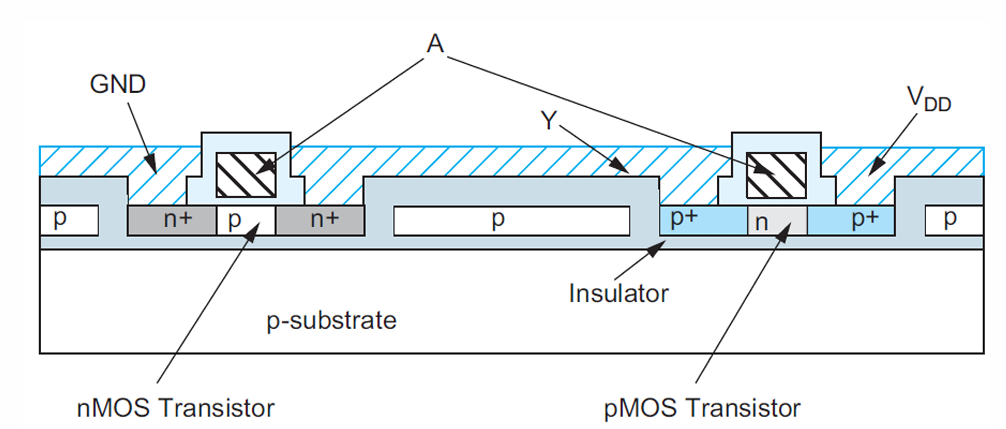
\includegraphics[width=\textwidth]{img/TX_img/soi.png}
        \caption{SOI}
        \label{}
    \end{subfigure}
    \hfill
    % --- Subfigure (b) ---
    \begin{subfigure}{0.5\linewidth}
        \centering
        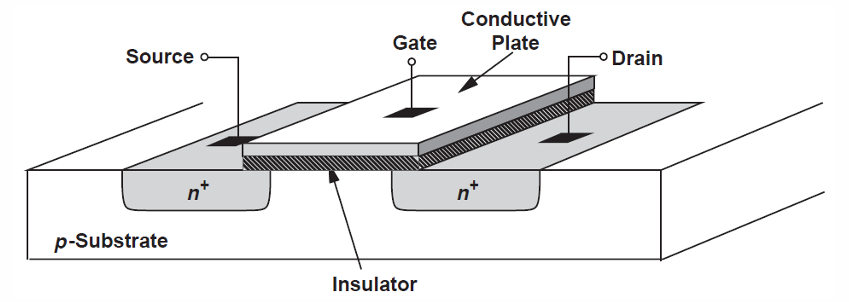
\includegraphics[width=\textwidth]{img/TX_img/bulk.png}
        \caption{Bulk MOSFET}
        \label{}
    \end{subfigure}
    \hfill
    \vspace{0.3cm}
    \caption{}
    \label{fig:NRZ SST}
\end{figure}
\section{Comparative Analysis: Regular Well vs. Flip-Well Architecture}

The 22nm FD-SOI technology offers two primary well configurations, each providing different biasing capabilities for N-FET and P-FET devices:

\subsection{Regular Well (Standard Well)}
In a standard configuration, transistors are placed over wells of the opposite doping type (N-FET in a P-well, P-FET in an N-well).
\begin{itemize}
    \item \textbf{Biasing Type}: Primarily optimized for \textbf{Reverse Body Biasing (RBB)}.
    \item \textbf{Operation}: Applying the lowest voltage to the P-well increases the threshold voltage ($V_{th}$), which significantly reduces leakage power at the cost of switching speed.
    \item \textbf{Use Case}: Ideal for low-power blocks where leakage reduction is more critical than high-speed performance.
\end{itemize}

\subsection{Flip-Well (Flipped-Well)}
In a Flip-Well architecture, the doping polarities of the underlying wells are reversed, placing transistors over wells of the same doping type (N-FET in an N-well, P-FET in a P-well).
\begin{itemize}
    \item \textbf{Forward Body Biasing (FBB)}: This configuration allows for aggressive Forward Body Biasing, often exceeding $2\,$V.
    \item \textbf{Performance Boost}: FBB significantly lowers the $V_{th}$ and increases the drive current ($I_{on}$), which is essential for reaching the high data rates required by the PCIe SERDES.
    \item \textbf{Tunability}: It enables a "tunable" transistor that can transition between high-performance modes and low-leakage idle states.
    
\end{itemize}

\begin{table}[htbp]
    \centering
    \caption{Strategic Differences Between Regular and Flip-Well FD-SOI}
    \label{tab:well_comparison}
    \begin{tabular}{l l l}
        \toprule
        \textbf{Feature} & \textbf{Regular Well} & \textbf{Flip-Well} \\
        \midrule
        N-FET Placement & P-well & N-well \\
        P-FET Placement & N-well & P-well \\
        Primary Bias Mode & Reverse Body Bias (RBB) & Forward Body Bias (FBB) \\
        Threshold Voltage ($V_{th}$) & Increased (High $V_{th}$) & Decreased (Low $V_{th}$) \\
        Leakage & Lowered & Significantly Increased \\
 
        \bottomrule
    \end{tabular}
\end{table}

\begin{figure}[H]
    \centering
    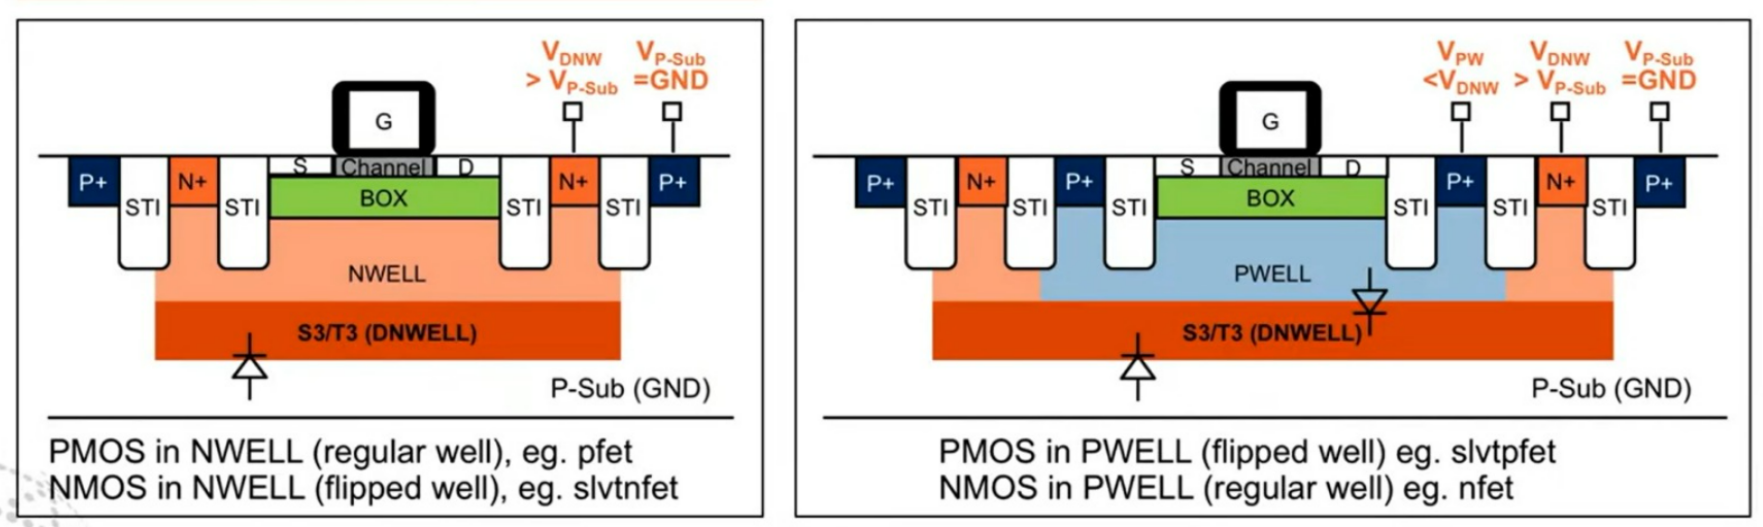
\includegraphics[width=1\textwidth]{img/TX_img/fwell.png}
    \caption{Structural illustration of Flip-Well vs. Conventional Well in FD-SOI.}
    \label{fig:flip_well}
\end{figure}





% ==================================================
% CHAPTER 2: FUNDAMENTALS & LIT REVIEW
% ==================================================
\chapter{System overview and Literature Architectures}
\label{ch:fundamentals}

\section{Clocking Systems in Wireline Transceivers}
\label{sec:clocking-systems}

In high-speed wireline communication, the clocking system is the "heartbeat" of the entire transceiver. Its primary function is to provide a precise time reference that dictates when data bits are generated, transmitted, and sampled. Without a highly stable clock, the synchronization between the transmitter (TX) Blocks would fail, leading to massive data corruption.

\subsection{The Role of Clocking in Serialization}
\label{subsec:role-clocking-serialization}

The most critical application of high-speed clocking within the transmitter is the \textbf{Serialization process}. In modern systems, data is processed internally in a parallel format (e.g., 32 or 64 bits wide) at a relatively low frequency to save power. To transmit this data over a single physical channel (like a copper trace or fiber), it must be converted into a serial bitstream.

The Serializer uses the clock signal to "multiplex" these parallel bits into a single high-speed line. For example, in a system aiming for a 64 Gbps data rate with 32Gbaud, the clocking network must provide timing edges that allow the serializer to place a new bit every \textbf{31.25 picoseconds}. Any misalignment or instability in this clock directly reduces the "eye opening" of the transmitted signal, making it harder for the receiver to distinguish between a digital '0' and '1'.

\begin{figure}[H]
    \centering
    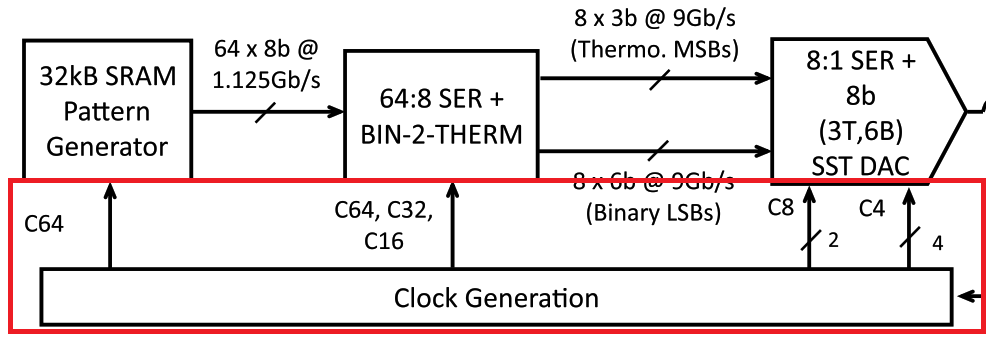
\includegraphics[width=0.8\textwidth]{img/TX_img/System.png}
    \caption{Clock Bundle in The System.}
    \label{fig:Wire Scaling}
\end{figure}

\section{Design Challenges in High-Frequency Clock Distribution}
\label{sec:design-challenges}

At a 32 GHz operating frequency, the clock period is \textbf{31.25 ps}. This extreme speed transforms the clock distribution network from a simple routing task into a complex high-frequency design problem. The challenges are primarily driven by the physical limitations of interconnects and the active circuitry required to drive them.

\subsection{Interconnect (Wire) Scaling and Bandwidth Limits}
\label{subsec:interconnect-scaling}

As CMOS technology scales to smaller nodes, the physical properties of on-chip metal wires become the dominant bottleneck.

\begin{itemize}
    \item \textbf{RC Delay and Scaling:} Every new technology node reduces the cross-sectional area of metal traces, which causes \textbf{Resistance (R)} to increase dramatically. Simultaneously, closer proximity to other wires increases parasitic \textbf{Capacitance (C)}. The resulting RC time constant of the wire limits how fast a signal can travel. At 32 GHz, even a relatively short wire can have a delay that is a significant fraction of the total clock period.
    
    \item \textbf{The RC-LPF Effect:} High-speed interconnects behave as a \textbf{Low-Pass Filter (LPF)}. This filter attenuates high-frequency components of the signal. Because a square-wave clock relies on high-frequency harmonics to maintain its shape, the wire "rounds off" the edges. By the time a 32 GHz signal travels across the transmitter, it loses its sharp transitions, making it difficult for the Serializer to detect valid clock edges.
\end{itemize}

\begin{figure}[H]
    \centering
    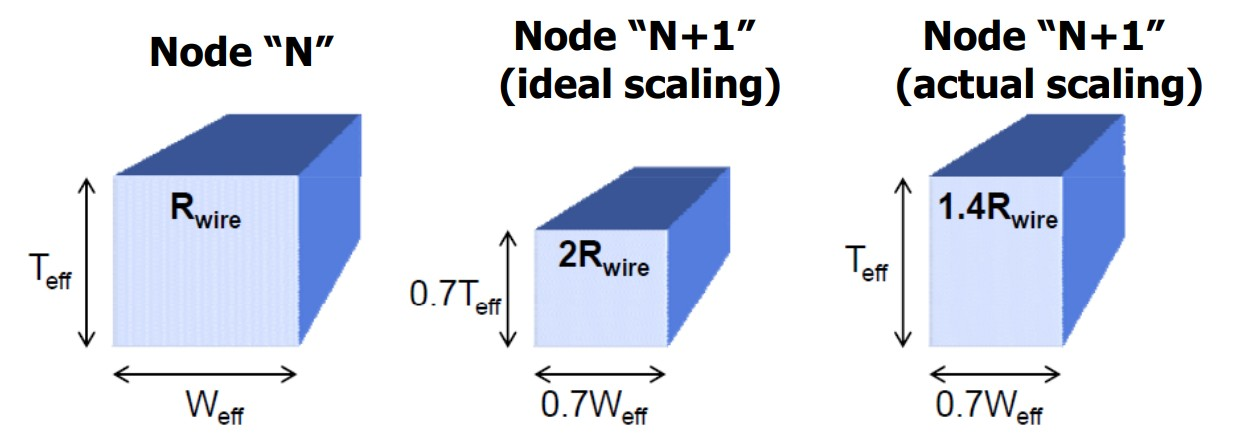
\includegraphics[width=0.7\textwidth]{img/TX_img/Wire_scaling.jpg}
    \caption{Impact of Technology Node Scaling on Wire Resistance and Geometry.}
    \label{fig:Wire Scaling}
\end{figure}


\subsection{Cascaded Clock Buffer Chains}
\label{subsec:cascaded-buffers}

Because the 32 GHz signal is severely attenuated by the\textbf{ LPF effect} and also increased delay due to wire resistance and the large capacitive load of the Serializer, it is physically impossible to drive the signal with a single buffer stage.

\begin{itemize}
    \item \textbf{The Repeater Strategy:} To maintain a usable voltage swing over the distance from the PLL to the Serializer, a chain of cascaded buffers must be placed along the path. These buffers act as "repeaters," re-amplifying the signal at regular intervals to combat the RC losses of the interconnects.
    
    \item \textbf{Load Management:} Each buffer must be sized to drive the input capacitance of the following stage. Since the GHz Serializer presents a massive capacitive load at an extremely high frequency, the final buffers in the chain must be exceptionally large. This results in significant power consumption and silicon area penalties.
\end{itemize}

\subsection{Jitter Amplification in Buffer Chains}
\label{subsec:jitter-amplification}

A major challenge with cascaded buffers at high frequencies is \textbf{Jitter Amplification}. This occurs when the clock frequency is close to the maximum bandwidth of the buffer.

\begin{itemize}
    \item \textbf{Limited Bandwidth Effect:} At 32 GHz, the clock period is so short (31.25 ps) that the transistors in the buffer may not have enough time to reach the full supply voltage (\(V_{DD}\)) or ground before the next transition begins. When the clock frequency operates close to the buffer's cutoff frequency, the buffer acts as a low-pass filter attenuating the signal and adds Jitter.
    
    \item \textbf{Noise-to-Jitter Conversion:} The limited bandwidth results in "rounded" edges with a slow \textbf{Slew Rate}. A slow slew rate is highly dangerous because it increases the \textbf{Rise} and \textbf{Fall} time of the signal. In this region, any small voltage noise (\(\Delta V\)) on the power supply or thermal noise from the transistors is translated into a large timing displacement (\(\Delta t\)), effectively "amplifying" the jitter.
    
    \item \textbf{Cumulative Degradation:} In a cascaded chain, each stage does not just pass the jitter of the previous stage; it adds its own noise and amplifies the existing timing uncertainty. By the time the 32 GHz clock reaches the Serializer, the accumulated jitter can consume a large portion of the Unit Interval (UI), leading to a significant increase in the Bit Error Rate (BER).
\end{itemize}

\begin{figure}[H]
    \centering
    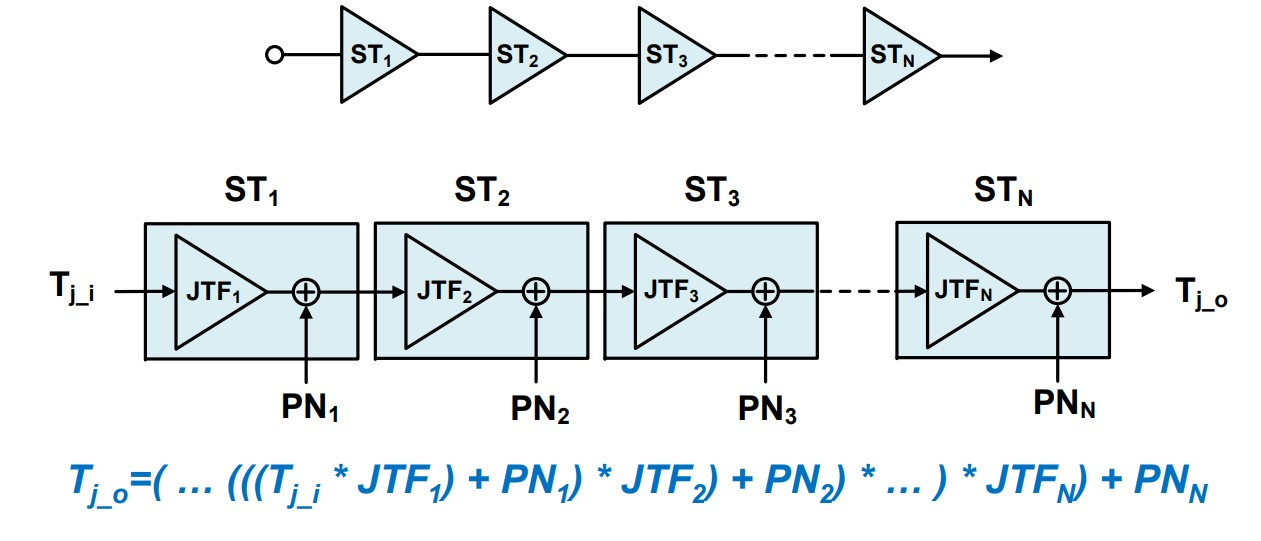
\includegraphics[width=0.8\textwidth]{img/TX_img/buffer_chain.jpg}
    \caption{Cumulative Jitter in Cascaded Clock Buffer Chains.}
    \label{fig:Wire Scaling}
\end{figure}

\subsection{Solution: Quadrature Clocking Scheme}
\label{sec:quadrature-solution}

To overcome the severe interconnect degradation and jitter amplification at High frequencies (eg. 32 GHz), modern high-speed transmitters utilize a \textbf{Quadrature Clocking Scheme}. This approach shifts the design strategy from "Brute Force" high-frequency distribution to a more efficient multi-phase architecture.

%\subsection{Frequency Reduction (Quarter-Rate Operation)}
%\label{subsec:frequency-reduction}
\begin{itemize}
    \item\textbf{Frequency Reduction (Quarter-Rate Operation):}

The most immediate benefit of the quadrature scheme is the reduction of the distribution frequency. By using four phases—\(0^\circ, 90^\circ, 180^\circ,\) and \(270^\circ\)—the system can operate at a "Quarter-Rate." which will effectively reduce \textbf {Power consumption} and \textbf{Jitter amplification}.

\begin{itemize}
    \item \textbf{Relaxed Bandwidth:} Instead of pushing a 32 $GHz$ signal through the buffer chains, the clocking blocks deliver an 8 GHz signal.
    
    \item \textbf{Combatting the RC-LPF:} At 8 GHz, the signal is much further away from the cutoff frequency of the on-chip interconnects. This results in significantly less amplitude attenuation and preserves the sharp edges of the clock, directly addressing the "Frequency Wall" mentioned in Section \ref{subsec:interconnect-scaling}.
\end{itemize}

\begin{figure}[H]
    \centering
    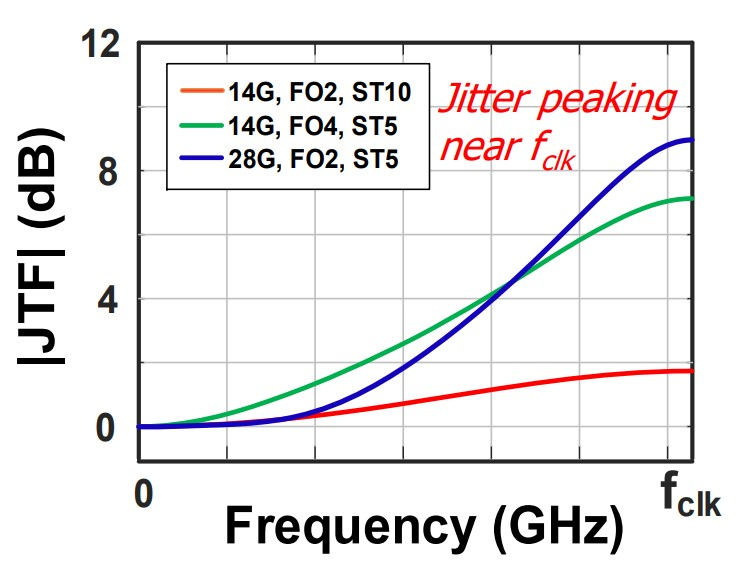
\includegraphics[width=0.8\textwidth]{img/TX_img/Jitter_amp.jpg}
    \caption{Jitter Transfer Function (JTF(dB)) vs. Clock Frequency.}
    \label{fig:Wire Scaling}
\end{figure}

\end{itemize}


%\subsection{Maintaining Data Throughput}
%\label{subsec:maintaining-throughput}
\begin{itemize}
    \item\textbf{Maintaining Data Throughput:}

The primary challenge in moving from a 32 GHz distribution to an 8 GHz distribution is maintaining the same data rate at the output The solution is not just using four phases, but specifically shaping those phases into a \textbf{25\% duty cycle}. This serves as the direct compensation for the slower clock speed.

\subsubsection{Replicating the 32 GHz Pulse Width}
In a full-rate 32 GHz system, each bit of data has a duration (Unit Interval or UI) of exactly 31.25 ps.

\begin{itemize}
    \item If we used a standard 8 GHz clock with a 50\% duty cycle, the "High" pulse would be \textbf{62.5 ps} long—twice as long as the required bit time.
    
    \item By enforcing a \textbf{25\% duty cycle} on the 8 GHz clock (\(125 \text{ ps} \times 0.25\)), we create a pulse that is exactly \textbf{31.25 ps} wide.
\end{itemize}

In this way, the 25\% duty cycle 8 GHz clock "mimics" the timing precision of the 32 GHz clock. It provides the exact same activation window for the serializer, but at a much lower repetition rate.

\subsubsection{Phase Interleaving for Full-Rate Throughput}
Because each 8 GHz phase now only occupies 25\% of the total cycle time, we can interleave four of these phases (\(0^\circ, 90^\circ, 180^\circ, 270^\circ\)) without any overlap.

\begin{itemize}
    \item Each phase is responsible for a different "time slot" in the 32 Gbps bitstream.
    
    \item As the first phase (\(0^\circ\)) finishes its 31.25 ps pulse, the second phase (\(90^\circ\)) immediately begins its 31.25 ps pulse.
\end{itemize}

This sequential "hand-off" between the four phases ensures that the Serializer is always active, producing a continuous stream of data at 32 Gbps. This effectively \textbf{compensates} for the 4\(\times\) reduction in frequency: the clock is 4\(\times\) slower, but because we use 4 phases with 1/4th the duty cycle, the data throughput remains identical to a 32 GHz system.

\subsubsection{Benefits of Compensation}
This compensation strategy allows the transmitter to enjoy the "best of both worlds":

\begin{enumerate}
    \item \textbf{Distribution Ease:} The wires and buffers only have to handle an 8 GHz fundamental frequency, avoiding the massive attenuation and quality loss of the 32 GHz "Frequency Wall" described in Section \ref{sec:design-challenges}.
    
    \item \textbf{Timing Accuracy:} The 25\% pulse width ensures the Serializer output maintains the correct bit period (\(31.25 \text{ ps}\)), preserving the "Data Eye" width for the receiver.
\end{enumerate}

\begin{figure}[H]
    \centering
    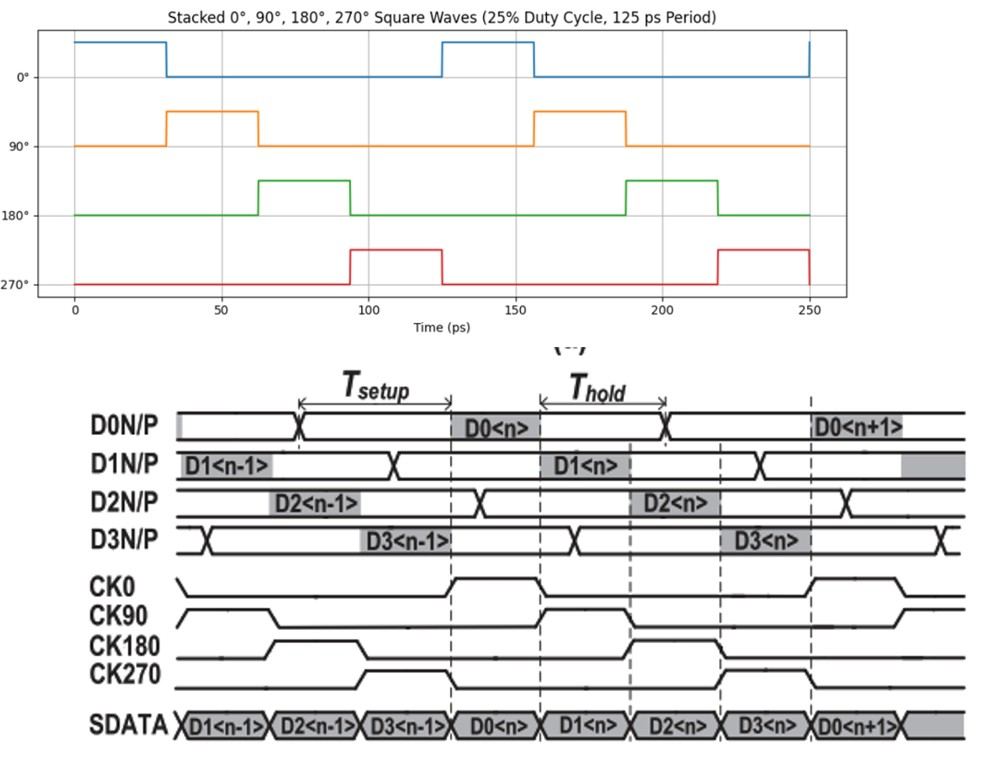
\includegraphics[width=0.8\textwidth]{img/TX_img/quarter_rate.jpg}
    \caption{Maintaining Data Throughput using Quarter Rate Clocking Scheme.}
    \label{fig:Wire Scaling}
\end{figure}

\end{itemize}

\section{Implementation Blocks for Quadrature Clocking}
\label{sec:implementation-blocks}

To implement a robust 8 GHz quadrature scheme, the transmitter clocking path integrates a series of specialized functional blocks. These blocks transform the raw high-frequency signal from the PLL into high-integrity timing pulses required by the Serializer.

\subsection{The I/Q Frequency Divider}
\label{subsec:iq-divider}

The I/Q Divider is the primary frequency translation element and the starting point of the local clock path.

\begin{itemize}
    \item \textbf{Function:} It receives the 32 GHz high-frequency reference from the PLL and divides it down to 8 GHz.
    
    \item \textbf{Quadrature Generation:} Utilizing a master-slave latch topology, it generates the four fundamental quadrature phases (\(0^\circ, 90^\circ, 180^\circ, 270^\circ\)) at a \textbf{50\% duty cycle}.
    
    \item \textbf{Challenges:} The divider must maintain high bandwidth to ensure that Division is done with low additional  jitter while operating at the limits of the technology node.
\end{itemize}

\subsection{Pulse Shaper (25\% Duty Cycle Generator)}
\label{subsec:pulse-shaper}

Since the I/Q divider produces 50\% duty cycle phases, a dedicated \textbf{Pulse Shaper} is required to prepare the clock for the quarter-rate serializer.

\begin{itemize}
    \item \textbf{Function:} This block performs a logic operation (typically an AND of overlapping quadrature phases) to reduce the pulse width from 50\% to \textbf{25\%}.
    
    \item \textbf{Frequency Compensation:} This creates the 31.25 ps window necessary to compensate for the reduced frequency, allowing the 8 GHz clock to drive a 32 Gbps bitstream with the same precision as a 32 GHz clock.
\end{itemize}

\subsection{Duty Cycle Correction (DCC) Circuits}
\label{subsec:dcc-circuits}

The DCC is a critical calibration block that maintains the integrity of the pulse width against PVT (Process, Voltage, Temperature) variations.

\begin{itemize}
    \item \textbf{50\% Correction Mode:} The DCC first ensures that the divider's outputs are perfectly symmetrical. If the 50\% duty cycle is distorted, it creates an immediate phase-shift error between the \(I\) and \(Q\) signals.
    
    \item \textbf{25\% Correction Mode:} The DCC also monitors the output of the Pulse Shaper. Because a 25\% pulse at 8 GHz is extremely narrow (31.25 ps), any drift can cause bit-width mismatch or data collisions in the Serializer. The DCC applies a correction voltage to "lock" the pulse width at exactly \(1/4\) of the clock period.
\end{itemize}

\subsection{Deskew Circuits}
\label{subsec:deskew-circuits}

The final block in the chain is the \textbf{Deskew} circuit, which provides the final "fine-tuning" of the timing edges.

\begin{itemize}
    \item \textbf{Function:} It provides independent delay control for each of the four quadrature phases.
    
    \item \textbf{Phase Orthogonality:} Even with a perfect divider, the physical metal routing to the Serializer can introduce "skew" (timing mismatches). Deskew circuits—usually digitally controlled delay lines—adjust the arrival of each phase to ensure they remain exactly \(90^\circ\) apart at the point of serialization.
    
    \item \textbf{System Impact:} This maximizes the horizontal timing margin (the "eye width") of the transmitted signal.
\end{itemize}

\subsection{Summary of Service}
\label{subsec:summary-service}

The I/Q Divider provides the raw phases, but open-loop division is susceptible to PVT (Process, Voltage, Temperature) variations. By including \textbf{DCC and Deskew circuits}, we create a robust clocking path that can calibrate itself to maintain 90\(^\circ\) precision and 50\% duty cycle regardless of manufacturing mismatches. This directly leads to a wider 'Data Eye' and a lower Bit Error Rate (BER) at the transmitter output.


\begin{table}[ht]
    \centering
    \caption{Quadrature Clocking Path Functional Blocks Summary}
    \label{tab:clocking-blocks}
    \begin{adjustbox}{width=\textwidth}
    \begin{tabular}{lcccc}
        \toprule
        \textbf{Block} & \textbf{Input Frequency} & \textbf{Output Frequency} & \textbf{Duty Cycle Focus} & \textbf{Primary Purpose} \\
        \midrule
        \textbf{I/Q Divider} & 16 GHz & \textbf{8 GHz} & 50\% & Frequency reduction \& \(I/Q\) generation \\
        \textbf{Pulse Shaper} & 8 GHz & \textbf{8 GHz} & 25\% & Frequency compensation (31.25 ps pulse) \\
        \textbf{DCC} & 8 \GHz & \textbf{8 \GHz} & 50\% \& 25\% & Preventing Duty Cycle Distortion (\DCD) \\
        \textbf{Deskew} & 8 \GHz & \textbf{8 \GHz} & Phase Alignment & Correcting routing-induced phase skew \\
        \bottomrule
    \end{tabular}
    \end{adjustbox}
\end{table}

\section{Jitter in High-Speed Clocking}
\label{sec:jitter-analysis}

Following the hardware implementation, it is essential to analyze the timing uncertainty, or jitter, that these blocks introduce. At 32 Gbps, jitter management is the primary factor in determining the system's reliability.

\subsection{Eye Diagram and Specification Mask}
\label{subsec:eye-diagram}

For proper operation, high-speed links must maintain margin in both the voltage and timing domains.

\begin{itemize}
    \item \textbf{Interoperability:} To allow independent design of the transmitter (TX) and receiver (RX), a "spec eye mask" is used, which is determined by the specific industry standard (e.g., PCIe, Ethernet).
    
    \item \textbf{Performance Guarantee:} The signal must not violate this mask to guarantee a minimum level of performance.
\end{itemize}

\begin{figure}[H]
    \centering
    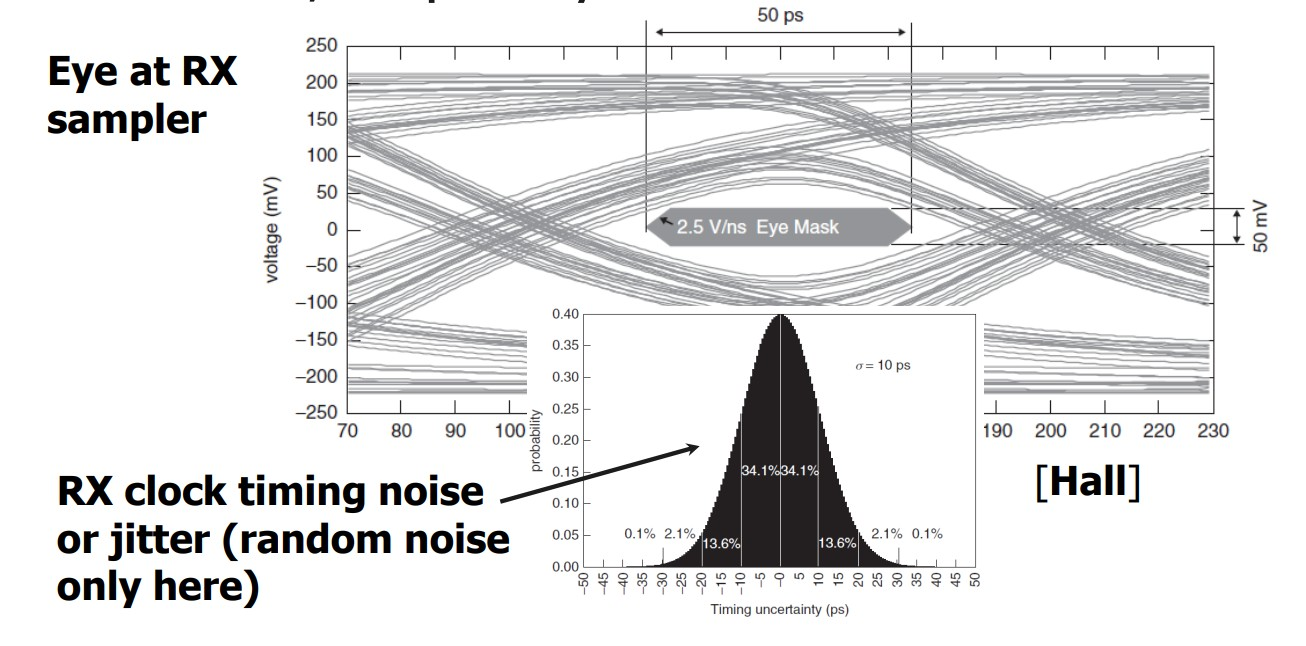
\includegraphics[width=0.8\textwidth]{img/TX_img/Eye_mask.jpg}
    \caption{Spec Mask.}
    \label{fig:Wire Scaling}
\end{figure}


\subsection{Jitter Definitions and Measurements}
\label{subsec:jitter-definitions}

Based on how we observe the signal, jitter is categorized into three measurement types:

\begin{itemize}
    \item \textbf{Period Jitter (\(J_{\text{PER}}\)):} The deviation of a single clock period from the ideal period (\(T_{\text{ideal}}\)). It is the most basic measure of clock stability.
    
    \item \textbf{Cycle-to-Cycle Jitter (\(J_{\text{CC}}\)):} The difference in duration between two consecutive clock periods. Important for budgeting on-chip digital circuits cycle time.
    
    \item \textbf{Accumulated Jitter (\(J_{\text{AC}}\)):} Also known as Long-Term Jitter, it measures the displacement of a clock edge relative to an ideal trigger after \(N\) cycles. This is the most critical metric for our transmitter, as it defines how much the clock drifts over the time required for serialization.
\end{itemize}

\begin{figure}[H]
    \centering
    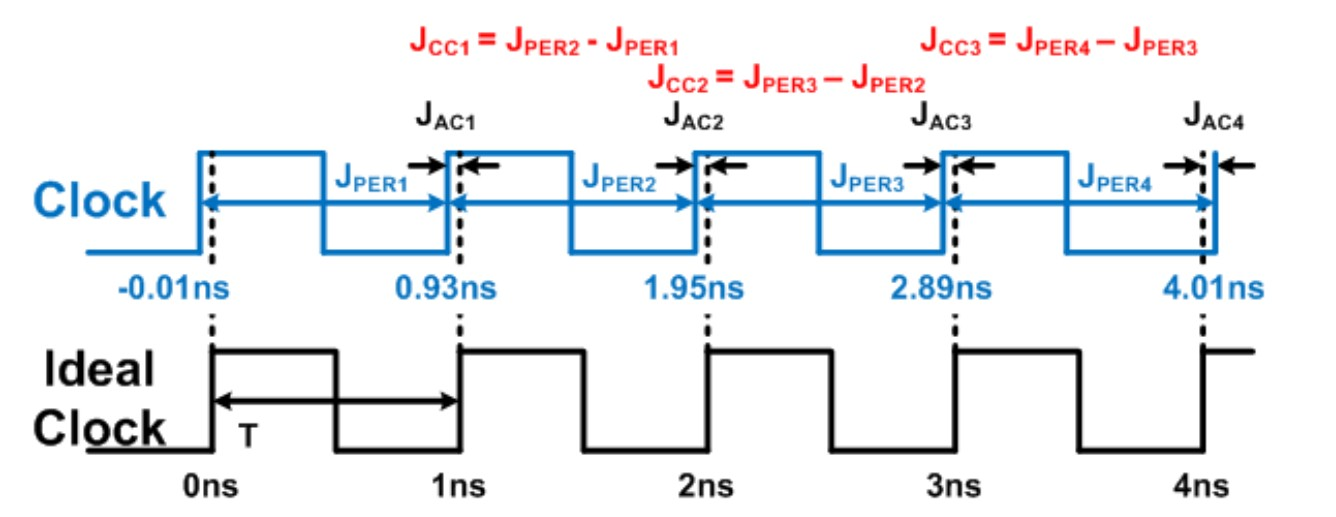
\includegraphics[width=0.8\textwidth]{img/TX_img/jitter_param.jpg}
    \caption{Jitter Definitions.}
    \label{fig:Wire Scaling}
\end{figure}

\subsection{Jitter Statistical Parameters}
\label{subsec:statistical-parameters}

Since jitter is a stochastic (random) process, we describe it using statistical metrics:

\begin{itemize}

\item \textbf{Mean Value:}
    Can be interpreted as a fixed timing offset or “skew”, Generally not important, as usually can corrected for.



    \item \textbf{RMS Jitter (\(\sigma\)):} The standard deviation of the jitter distribution. It is used to describe Random Jitter (\(\RJ\)).
    
    \item \textbf{Peak-to-Peak Jitter (\(J_{\text{PP}}\)):} Function of both deterministic (bounded) and random
    (unbounded) jitter components, Must be quoted at a given BER to account for random
    (unbounded) jitter.
    
\end{itemize}

\subsection{Detailed Classification of Jitter Components}
\label{subsec:jitter-classification}

Total Jitter (\(\TJ\)) is the result of various independent, correlated and uncorrelated noise sources. To manage a 64 Gbps link, we must categorize these components based on their statistical properties.

\subsubsection{Random Jitter (\(\RJ\))}
Random Jitter is timing noise that is unpredictable and follows a stochastic process.

\begin{itemize}
    \item \textbf{Sources \& Causes:}
    \begin{itemize}
        \item \textbf{Thermal Noise:} Generated by the random motion of electrons in conductors and transistors. It increases with temperature.
        \item \textbf{Flicker Noise (\(1/f\)):} Low-frequency noise caused by "traps" at the silicon-dielectric interface.
    \end{itemize}
    
    \item \textbf{Characteristics:}
    \begin{itemize}
        \item\ \textbf{unbounded}, follows a \textbf{Gaussian (Normal) Distribution} 
        \item\ Assumed to have zero mean value.
        \item\  It is quantified by its RMS value (\(\sigma\)).
    \end{itemize}
\end{itemize}

\begin{equation}
    \centering
    RJ(t) = \frac{1}{\sqrt{2\pi}\sigma_{RJ}} e^{\frac{-t^2}{2\sigma_{RJ}^2}}
\end{equation}

\begin{figure}[H]
    \centering
    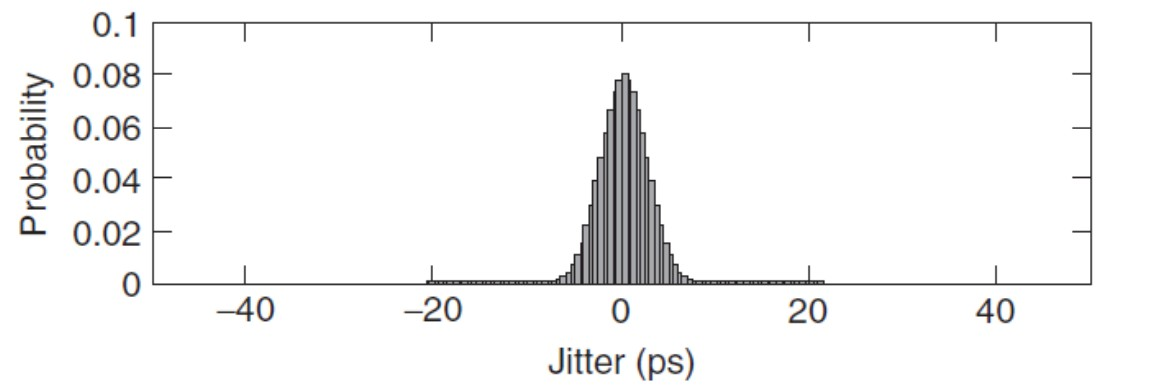
\includegraphics[width=0.8\textwidth]{img/TX_img/RJ.jpg}
    \caption{Probability Density Function (PDF) of Random Jitter.}
    \label{fig:Wire Scaling}
\end{figure}

\subsubsection{Deterministic Jitter (\(\DJ\))}
Deterministic Jitter is bounded; it has a specific maximum peak-to-peak value.
\begin{itemize}
    \item \textbf{causes:}
    \begin{itemize}
    \item \ Transmission-line losses (ISI)
    \item\ Duty Cycle Distortion (DCD)
    \item\ Spread Spectrum Clocking
    \item\ Crosstalk
    \end{itemize}
\end{itemize}

\begin{figure}[H]
    \centering
    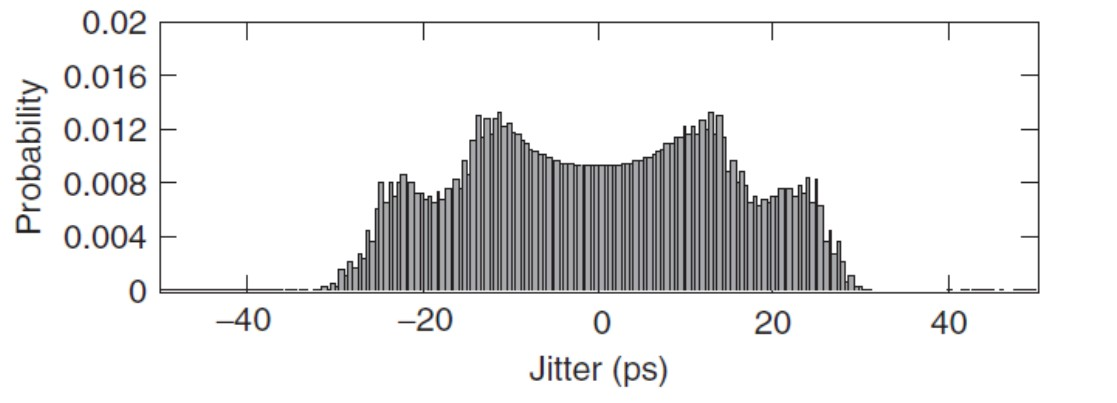
\includegraphics[width=0.8\textwidth]{img/TX_img/DJ.jpg}
    \caption{Probability Density Function (PDF) of Determinstic Jitter.}
    \label{fig:Wire Scaling}
\end{figure}

\subsubsection{Sinusoidal or Periodic Jitter (SJ or PJ):} 
Repeats at a fixed frequency due to modulating effects.

\begin{itemize}
    \item \textbf{Spread spectrum clocking:}
    \item \textbf{PLL reference clock feedthrough:}
\end{itemize}

\begin{equation}
    \centering
    PDF_{SJ}(t) = 
    \begin{cases} 
      \frac{1}{\pi\sqrt{A^2 - t^2}} & A > |t| \\
      0 & A \leq |t| 
    \end{cases}
\end{equation}

\begin{figure}[H]
    \centering
    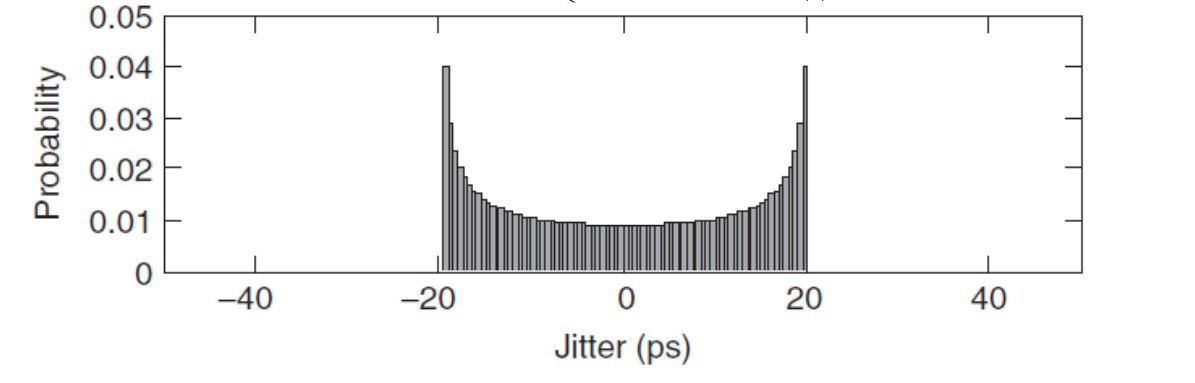
\includegraphics[width=0.8\textwidth]{img/TX_img/SJ.jpg}
    \caption{Probability Desity Function (PDF) of Sinusoidal Jitter.}
    \label{fig:Wire Scaling}
\end{figure}

\subsubsection{Data-Dependent Jitter (DDJ):}
    Data dependent jitter is correlated with either the transmitted data pattern or aggressor (crosstalk).

\begin{itemize}
    \item \textbf{Intersymbol Interference (ISI):}
    \begin{itemize}
        \item \textbf{Source:} Caused by channel loss, dispersion, and reflections.
        \item \textbf{Cause:} As discussed in the 32 GHz challenges, the RC-LPF effect prevents the signal from reaching full rail-to-rail swing before the next transition. The "memory" of previous bits shifts the threshold crossing point of the current bit.
        \item Can be improved by equalitzation.

\begin{figure}[H]
    \centering
    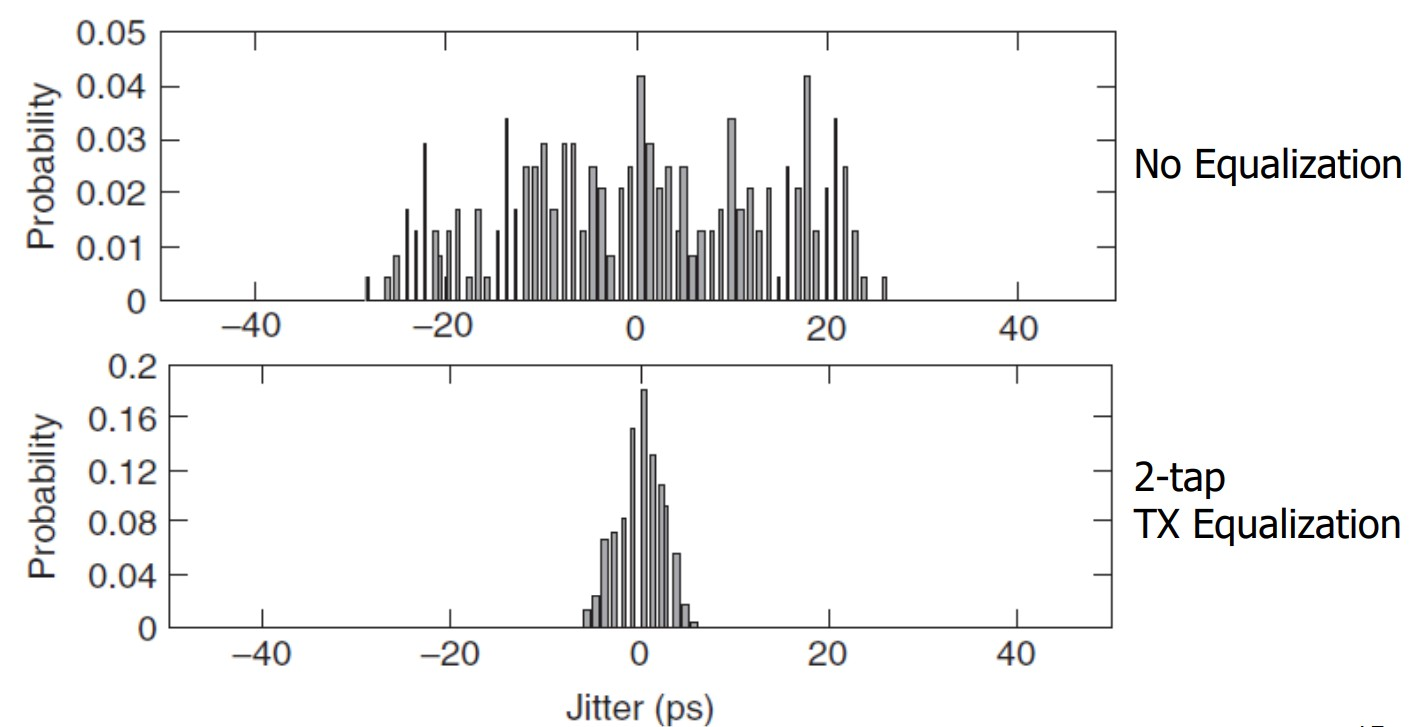
\includegraphics[width=0.8\textwidth]{img/TX_img/ISI.jpg}
    \caption{Probability Density Function (PDF) Of Inter-Symbol Interference Jitter.}
    \label{fig:Wire Scaling}
\end{figure}
        
    \end{itemize}
\end{itemize}

\begin{itemize}
    \item \textbf{Duty Cycle Distortion (DCD):}
    \begin{itemize}
        \item \textbf{Source:} Caused by duty cycle errors in TX serialization clocks and rise/fall delay mismatches.
        \end{itemize}
       \begin{itemize}
        \item \textbf{Rise/Fall Time Mismatch:} The buffers driving the output often have different slew rates for rising and falling edges. This is primarily caused by unequal strengths (W/L ratios) or switching speeds between PMOS and NMOS transistors.
        \item \textbf{Voltage Offsets:} DC offsets in the differential signals of the I/Q divider, often due to process variations or threshold voltage (\(V_{\text{th}}\)) mismatches, cause the signal to cross the switching threshold earlier or later than intended.
    \end{itemize}
    \item \textbf{Effect:}
    \begin{itemize}
        \item \textbf{Window Shrinkage:} DCD deviates the clock from the ideal 50\% or 25\% duty cycle. This results in the "sampling" windows for the four quadrature phases being unequal in width.
        \item \textbf{Bit-Width Mismatch:} One bit in the 32 Gbps stream becomes wider while the next becomes narrower. This "non-ideal zero-crossing" reduces the horizontal timing margin (eye-width), making the system highly sensitive to error at the Serializer output.
    \end{itemize}
\end{itemize}


\begin{equation}
    \centering
    PDF_{DCD}(t) = \frac{1}{2} \left[ \delta\left(t - \frac{\alpha_{DCD}}{2}\right) + \delta\left(t + \frac{\alpha_{DCD}}{2}\right) \right]
\end{equation}

\begin{figure}[H]
    \centering
    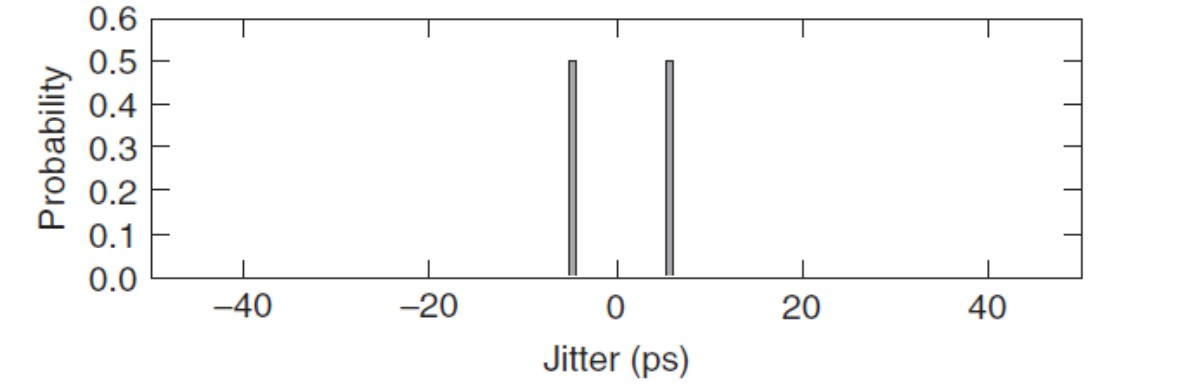
\includegraphics[width=0.8\textwidth]{img/TX_img/DCD.jpg}
    \caption{Probability Desity Function (PDF) of Duty Cycle Distortion Jitter.}
    \label{fig:Wire Scaling}
\end{figure}


\begin{itemize}
\item \textbf{Bounded Uncorrelated Jitter (BUJ):}


\begin{itemize}
    \item \textbf{Source:} Primarily \textbf{Crosstalk}.
    \item \textbf{Cause:} When a nearby high-speed signal (aggressor) switches, it injects a current spike into the clock line (victim) via mutual capacitance or inductance.
    \item \textbf{Characteristics:} It is "Uncorrelated" because the aggressor's data usually has no relationship with the clock, but it is "Bounded" because the interference has a maximum physical limit.
    \end{itemize}
\end{itemize}


\subsection{Total Jitter (TJ)}
The total jitter PDF is produced by convolving the random and deterministic jitter PDFs.
The Total Jitter (TJ) represents the overall timing uncertainty in the system. The probability density function (PDF) of total jitter is mathematically derived by convolving the individual PDFs of random and deterministic jitter components:

\begin{equation}
    PDF_{JT}(t) = PDF_{RJ}(t) * PDF_{DJ}(t)
\end{equation}

where the deterministic jitter PDF is itself a result of the convolution of several sub-components, including Periodic (Sinusoidal) Jitter ($SJ$), Duty Cycle Distortion ($DCD$), Intersymbol Interference ($ISI$), and Bounded Uncorrelated Jitter ($BUJ$):

\begin{equation}
    PDF_{DJ}(t) = PDF_{SJ}(t) * PDF_{DCD}(t) * PDF_{ISI}(t) * PDF_{BUJ}(t)
\end{equation}

\begin{figure}[H]
    \centering
    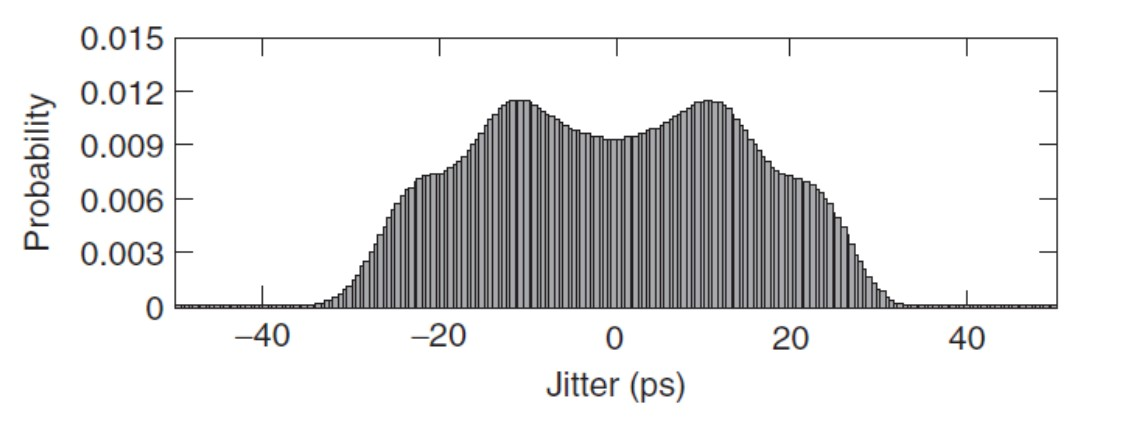
\includegraphics[width=0.8\textwidth]{img/TX_img/TJ.jpg}
    \caption{Probability Desnity Function (PDF) of Total Jitter .}
    \label{fig:Wire Scaling}
\end{figure}


\subsection{System Jitter Budgeting}
\label{subsec:jitter-budgeting}

Jitter budgeting is the mathematical process used to ensure that the cumulative timing uncertainty from all sources—transmitter, clock distribution, and channel—does not exceed the Unit Interval (UI). To guarantee a specific Bit Error Rate (BER), jitter components must be combined according to their statistical nature.

\subsubsection{Linear Addition of Deterministic Jitter (\(\DJ\))}
Deterministic Jitter components are bounded and have fixed peak-to-peak values. The convolution of multiple bounded jitter distributions is approximated by the linear sum of their individual peak-to-peak terms:

\begin{equation}
    D_{J,\text{total}} = \sum D_{J,i} = D_{J,\text{ISI}} + D_{J,\text{DCD}} + D_{J,\text{Pj}} + \cdots
\end{equation}

Since \(\DJ\) is not random, every pico second of deterministic jitter added to the system directly reduces the available timing window for sampling.

\subsubsection{Root-Sum-Square (RSS) of Random Jitter (\(\RJ\))}
Random jitter sources (such as thermal and shot noise) are uncorrelated and follow a Gaussian distribution. To calculate the total system \(\RJ\), the RMS values are combined using the RSS method:

\begin{equation}
    \sigma_{\RJ,\text{total}} = \sqrt{\sigma_{\RJ,1}^2 + \sigma_{\RJ,2}^2 + \sigma_{\RJ,3}^2 + \cdots}
\end{equation}

This statistical approach is used because it is highly improbable for multiple independent random noise sources to reach their peak displacement simultaneously.

\subsubsection{Total Jitter (TJ) and the Dual-Dirac Model}
The Dual-Dirac model is the industry standard for predicting eye closure at a specific BER. It combines the bounded \(\DJ\) and the unbounded Gaussian \(\RJ\):

\begin{equation}
    T_J(\text{BER}) = D_{J,pp} + Q(\text{BER}) \cdot \sigma_{R_J,total}
\end{equation}

\begin{itemize}
    \item \textbf{The Q-Factor:} This multiplier represents the number of standard deviations required to achieve a target probability on the Gaussian tails.
    
    \item \textbf{The \(14\sigma\) Rule:} For a common target of BER = \(10^{-12}\), the \(Q\) factor is approximately 14 (representing \(7\sigma\) on each side of the transition). In this case, the equation becomes:
    \end{itemize}
    
   \begin{equation}
    T_J = D_{J,pp} + 14 \cdot \sigma_{R_J,total}
\end{equation}

\subsubsection{The Timing Margin Requirement}
A high-speed link is considered functional only if the Total Jitter is less than the Unit Interval, leaving sufficient margin for the receiver:

\begin{equation}
    \UI \geq \TJ(\BER) + \text{Receiver Margin}
\end{equation}

If the total jitter exceeds the UI, the "Data Eye" closes, and the receiver will be unable to distinguish between bit transitions, leading to a failure to meet the BER target. Design techniques such as Duty Cycle Correction (DCC) and Deskewing are employed specifically to reclaim this timing margin by minimizing the \(\DJ\) components.

\begin{figure}[H]
    \centering
    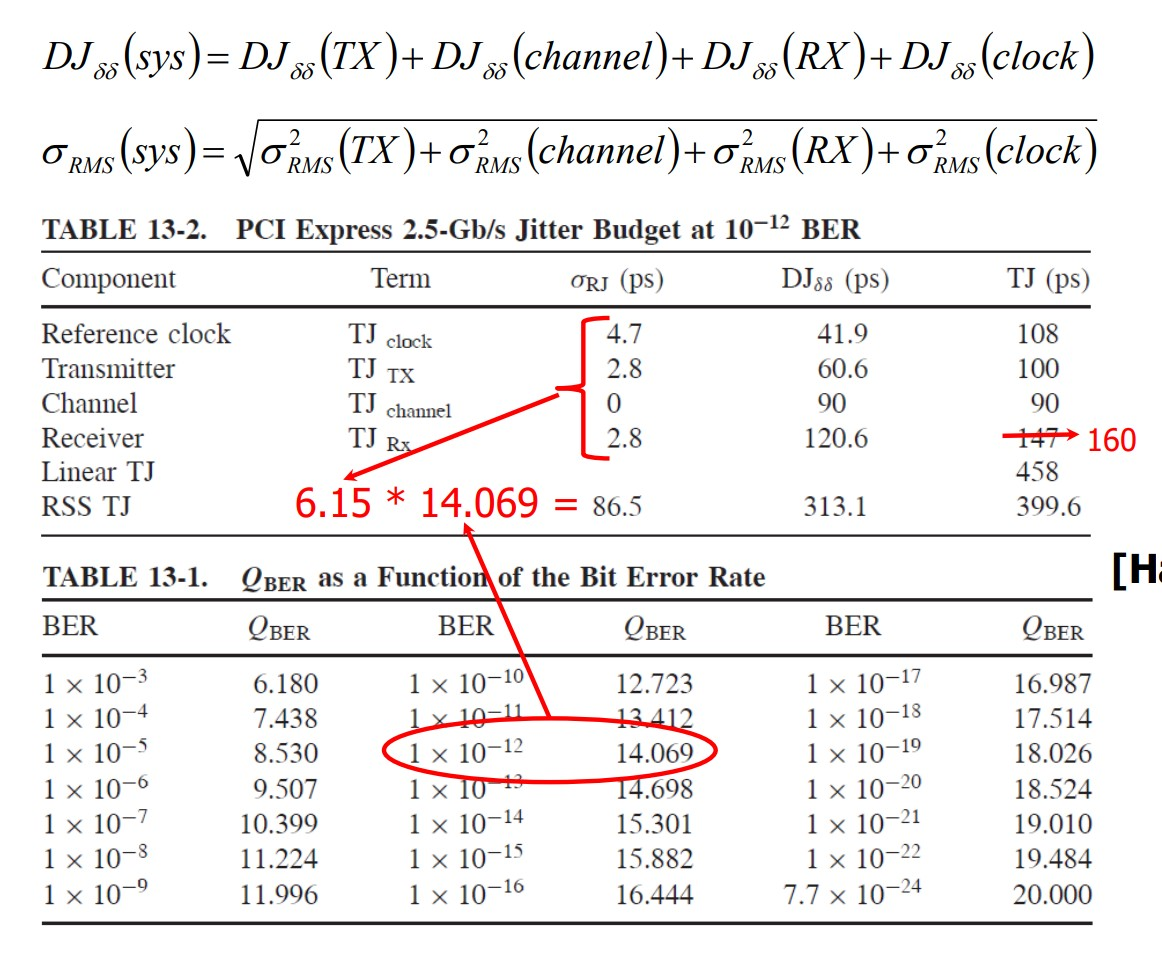
\includegraphics[width=0.8\textwidth]{img/TX_img/Jitter_ex.jpg}
    \caption{Jitter budgeting Example.}
    \label{fig:Wire Scaling}
\end{figure}


% ==================================================
% CHAPTER 1: INTRODUCTION
% ==================================================
\setcounter{page}{1}   % Reset counter to 1 for the Introduction
\section{Fundamentals of High-Speed Serialization}
The core function of a high-speed transmitter is to convert parallel low-speed data from the digital core into a serial high-speed stream suitable for transmission over the physical medium. This Parallel-In Serial-Out (PISO) operation is the final and most critical stage of the digital-to-analog interface. As data rates scale towards 64 Gb/s and beyond, the serializer (Multiplexer or Mux) becomes the primary bandwidth bottleneck. This chapter reviews the fundamental serialization architectures and presents a literature survey of circuit topologies used to implement the high-speed multiplexer.

\subsection{The Parallel-In Serial-Out (PISO) Concept}
A PISO block receives $N$ parallel data streams, each running at a frequency of $f_{clk}/N$, and interleaves them into a single serial stream running at the full baud rate $f_{baud}$. In the context of PAM4 signaling, the serializer operates on symbols rather than individual bits. For a 64 Gb/s PAM4 link, the symbol rate is 32 Gbaud.

The design of the PISO stage is governed by the trade-off between the complexity of the clock distribution network and the switching speed of the multiplexing circuits.

\begin{figure}[H]
    \centering
    % REPLACE 'piso.jpg' with your filename
    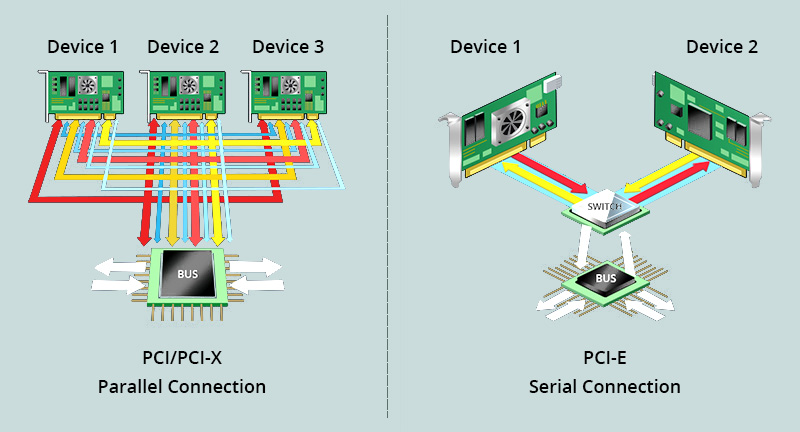
\includegraphics[width=0.8\textwidth]{img/TX_img/piso.jpg}
    \caption{Conceptual operation of the Parallel-In Serial-Out (PISO) block: Converting parallel low-speed data streams into a single high-speed serial output.}
    \label{fig:piso_diagram}
\end{figure}
\clearpage
\subsection{System-Level Placement of the : 4:1 High-Speed Multiplexer and Pre-Driver}
\label{subsec:system_level_placement_mux}

The high-speed multiplexer (MUX) and integrated pre-driver chain serve as the final digital stage within the transmitter serialization architecture. Positioned at the very end of the digital serialization domain, this integrated macro links the low-speed digital core with the high-speed analog front-end macros. 

\subsubsection{Data Path Context and Interface Boundaries}

The data path position of this macro is defined by its incoming and outgoing interface parameters:
\begin{itemize}
    \item \textbf{Input Interface:} The block receives 4 parallel lanes from the upstream digital serialization core (post-64:4 digital core serialization) with an input symbol period of $125\text{ ps}$.
    \item \textbf{Output Interface:} The core multiplexer logic merges these parallel streams into a single serial stream, which is delivered directly to the analog output stage with a compressed symbol period of $31.25\text{ ps}$.
\end{itemize}

\begin{figure}[H]
    \centering
    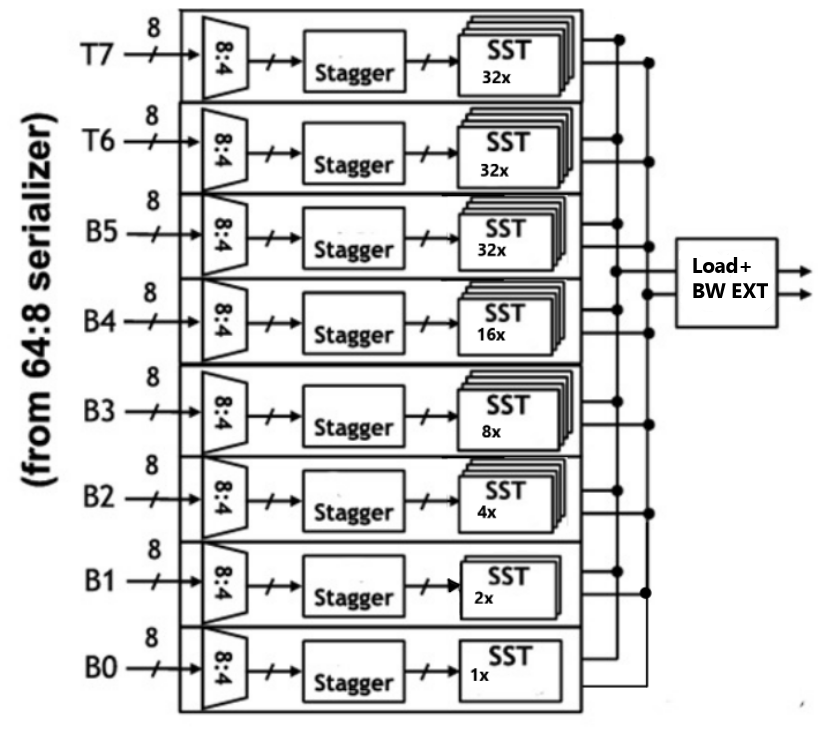
\includegraphics[width=0.9\textwidth]{img/TX_img/dac_based_architecture.png}
    \vspace{1mm} 
    \caption{Architectural overview of the DAC-Based Transmitter.}
    \label{fig:transmitter_macro_overview}
\end{figure}

\subsubsection{Timing Constraints}

Because the output data tracks run with a symbol period of $31.25\text{ ps}$, this integrated block is the fastest digital section in the entire transmitter macro. The physical routing channels and stage transitions must handle picosecond-level timing budgets to preserve the integrity of the data stream. 

To satisfy these tight timing constraints, the staggered 4-bit parallel data ($D4\langle0:3\rangle$) is fed into a high-speed 4:1 multiplexer core before driving the active pre-driver staging, which provides the necessary signal sharpening to drive the final source-series terminated (SST) analog driver stage.

\begin{figure}[H]
    \centering
    % Place holder for the 4:1 MUX -> Pre -> SST block slice diagram
     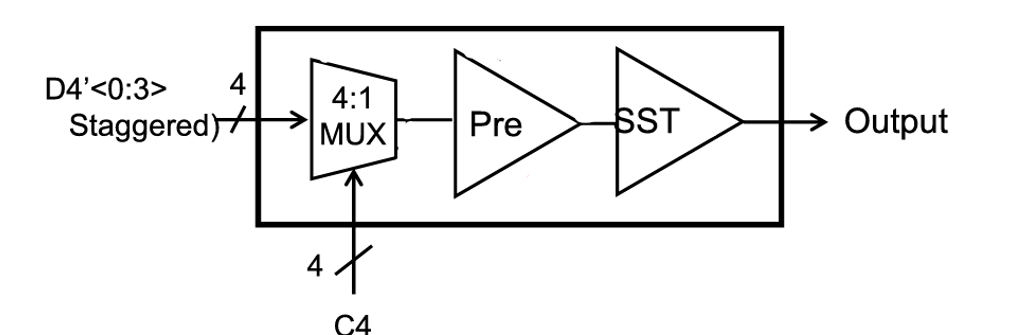
\includegraphics[width=0.75\textwidth]{img/TX_img/mux_predriver_sst_slice.png}
    \vspace{1mm} 
    \caption{Detailed schematic slice of the standalone serialization branch showing the 4:1 multiplexer cell, active pre-driver buffers, and the analog output driver.}
    \label{fig:mux_predriver_sst_slice}
\end{figure}

\subsection{Serialization Rate Architectures}
To achieve a target symbol rate of 32 Gbaud (for 64 Gb/s PAM4), three primary clocking architectures are typically discussed in literature: Full-Rate, Half-Rate, and Quarter-Rate.

\subsubsection{Full-Rate Architecture}
In a Full-Rate architecture, the serializer is driven by a clock frequency equal to the output symbol rate. For a 32 Gbaud link, this requires a 32 GHz clock signal.

\begin{itemize}
    \item \textbf{Operation:} The circuit retimes the data on every rising edge of the clock, requiring the latching elements to operate at the fundamental frequency of the data stream.
    \item \textbf{Limitations:} The primary bottleneck of this topology is the stringent timing budget. The entire serialization operation—including the clock-to-output delay ($t_{c-q}$) and the setup time ($t_{setup}$)—must complete within a single Unit Interval (UI). As data rates scale, the UI shrinks (e.g., only 31.25 ps at 32 Gbaud), leaving vanishingly small margins for process variations or jitter.
\end{itemize}

\subsubsection{Half-Rate Architecture}
Half-Rate architectures utilize a clock frequency at half the baud rate (16 GHz for 32 Gbaud).
\begin{itemize}
    \item \textbf{Operation:} Data is sampled on both the rising and falling edges of the clock (Double Data Rate or DDR). This effectively acts as a 2:1 multiplexer in the final stage.
    \item \textbf{Limitations:} While it relaxes the clock frequency, Half-Rate architectures are highly sensitive to Duty Cycle Distortion (DCD). If the clock duty cycle deviates from exactly 50\%, the ``even'' symbols will have a different width than the ``odd'' symbols, directly closing the eye diagram horizontally.
\end{itemize}

\subsubsection{Quarter-Rate Architecture}

Quarter-Rate architectures utilize a clock frequency at one-quarter of the baud rate (e.g., 8 GHz for 32 Gbaud). This approach further relaxes the timing constraints on the latching elements but increases the complexity of the clock generation and distribution network.

\begin{itemize}
    \item \textbf{Operation:} The serializer functions as a 4:1 multiplexer, combining four parallel low-speed data streams into a single high-speed output. This requires four clock phases spaced 90$^{\circ}$ apart ($\Phi_0, \Phi_{90}, \Phi_{180}, \Phi_{270}$) to sequentially select the input bits.

    \item \textbf{Duty Cycle Selection:} A critical design distinction in Quarter-Rate topologies is the choice between 50\% and 25\% clock duty cycles.
    \begin{itemize}
        \item \textit{50\% Duty Cycle:} Standard quadrature clocks naturally have a 50\% duty cycle, meaning each phase is active for 2 Unit Intervals (UI). Since the target bit period is 1 UI, adjacent clock phases inherently overlap. Using these directly would cause signal contention (short circuits) at the multiplexer output.
        \item \textit{25\% Duty Cycle (Selected):} To eliminate contention, this implementation utilizes a \textbf{25\% duty cycle} scheme. By reducing the pulse width to exactly 1 UI, the four clock phases become strictly non-overlapping. This ensures that only one slice drives the output at any given instant, allowing for robust serialization without the need for additional gating logic.
    \end{itemize}
\end{itemize}
\begin{figure}[H]
    \centering
    % REPLACE 'piso.jpg' with your filename
    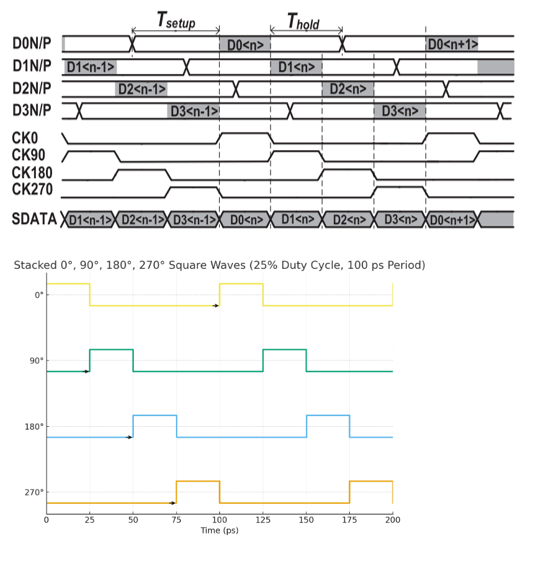
\includegraphics[width=0.8\textwidth]{img/TX_img/core idea.png}
    \caption{Timing diagram of the Quarter-Rate serialization scheme. The lower waveforms depict the proposed 25\% duty cycle clock phases ($0^\circ, 90^\circ, 180^\circ, 270^\circ$), which create strictly non-overlapping selection windows to sequentially serialize the parallel input data ($D_0-D_3$) without signal contention.}
    \label{fig:quarter_rate_timing}
\end{figure}

% =========================================================
% REVISED LITERATURE REVIEW (Neutral & Professional)
% =========================================================
\section{Literature Review of Multiplexer Topologies}

The design of the final 4:1 multiplexer stage is critical for signal integrity. Over the past decade, three primary circuit topologies have dominated the literature for high-speed serialization: Transmission Gates (TG), Current-Mode Logic (CML), and CMOS Tri-State Logic. This section surveys their operating principles and performance trade-offs in the context of high-speed PAM4 signaling.

\clearpage

\subsection{Transmission Gate (TG) based Topology}
The CMOS Transmission Gate (TG) functions as a high-speed passive switch, utilizing parallel NMOS and PMOS devices to pass the signal from input to output.

\begin{figure}[H]
    \centering
    % REPLACE 'piso.jpg' with your filename
    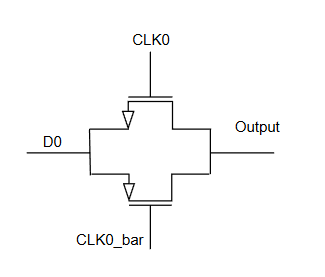
\includegraphics[width=0.5\textwidth]{img/TX_img/tg.png}
    \caption{Simple Schematic diagram of a CMOS Transmission Gate (TG) switch used in high-speed multiplexers.}
    \label{fig:tg_schematic}
\end{figure}

\begin{itemize}
    \item \textbf{Advantages:} The primary appeal of the TG topology is its zero static power consumption. Since it contains no direct path from supply to ground, it is theoretically the most power-efficient architecture for low-frequency applications.
    \item \textbf{Limitations:} As reviewed in recent literature, TG-based muxes face severe challenges at high data rates . The "Self-Loading" effect becomes dominant: to reduce the on-resistance ($R_{on}$), the transistor width must be increased, which inevitably increases the parasitic capacitance ($C_{par}$). This creates a fundamental bandwidth limit.
\end{itemize}
\newpage
\subsection{Current-Mode Logic (CML) based Topology}
Current-Mode Logic (CML) relies on Data an clock logical combination to generate the output.
\begin{figure}[H]
    \centering
    % REPLACE 'piso.jpg' with your filename
    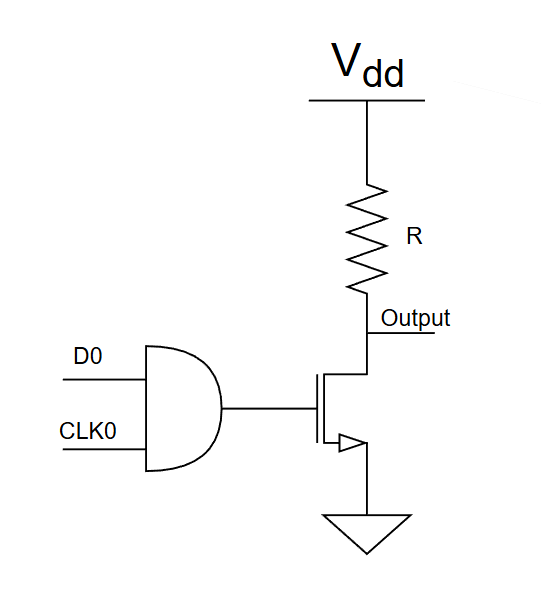
\includegraphics[width=0.5\textwidth]{img/TX_img/cml slice.png}
    \caption{Schematic of a Current-Mode Logic (CML) driver stage with a resistive load. In this implementation, the data ($D_0$) is logically combined with the clock ($CLK_0$) to gate the NMOS driver, allowing current to passthrough the load resistor $R$ only during the active phase.}
    \label{fig:cml_schematic}
\end{figure}
\begin{itemize}
    \item \textbf{Advantages:} CML is widely regarded in literature as the fastest logic family. Its differential nature provides excellent common-mode noise rejection, and its low voltage swing enables extremely fast switching speeds, making it a standard choice for optical and 100G+ interfaces.
    \item \textbf{Limitations:} The major drawback of CML is its high static power consumption, which occurs even when the data is not switching. Furthermore, the output swing is limited by the $I_{tail} \times R_{load}$ product. Achieving a high swing for acceptable SNR requires a large tail current or large load resistors, both of which degrade the power-bandwidth trade-off.
\end{itemize}
\newpage
\subsection{Active Tri-State Inverter based Topology}
The Tri-State inverter topology utilizes a clocked inverter structure (a stack of series transistors) to actively drive the output node.
\begin{figure}[H]
    \centering
    % Keeping the size consistent with the CML figure
    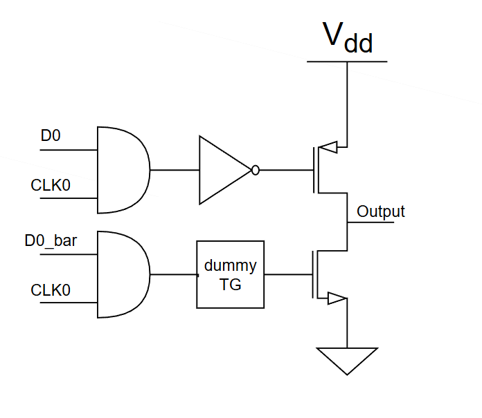
\includegraphics[width=0.5\textwidth]{img/TX_img/tri_slice.png}
    
    \caption{Schematic implementation of the Active Tri-State Inverter branch. The data inputs ($D_0$ and $\overline{D_0}$) are logically AND-ed with the clock phase ($CLK_0$). This ensures that both the PMOS and NMOS transistors are turned OFF (High-Impedance state) when the clock is inactive, preventing contention with other branches.}
    \label{fig:tristate_schematic_implementation}
\end{figure}

\begin{itemize}
    \item \textbf{Advantages:} Unlike the TG, the Tri-State topology is "active," meaning it regenerates the signal levels. This allows for a full rail-to-rail voltage swing, which maximizes the vertical and horizontal eye opening and.
    \item \textbf{Limitations:} The primary challenge documented in literature is Dynamic Power consumption. Since power scales with $CV^2f$, driving a full-swing signal at 64 Gb/s results in significant dynamic energy dissipation. Additionally, this topology is susceptible to "shoot-through" current (short-circuit power) during the brief moments when both PMOS and NMOS networks are partially on, requiring precise timing control of the clock phases.
\end{itemize}
\newpage
% =========================================================
% SECTION 2.3: SELECTION & ANALYSIS
% =========================================================
\section{Architecture Selection and Comparative Analysis}
\label{sec:arch_selection}

Following the review of available topologies, this section presents a comparative analysis based on the critical metrics for a 64 Gb/s PAM4 transmitter: Bandwidth, Power Consumption, jitter and Output Swing.

\subsection{Comparative Performance Metrics}
Table \ref{tab:topology_comparison} summarizes the trade-offs between the Transmission Gate (TG), Current-Mode Logic (CML), and Active Tri-State Inverter topologies based on recent literature in 22nm and similar nodes.

\begin{table}[htbp]
    \centering
    \caption{Comparative Analysis of Multiplexer Topologies for High-Speed SerDes}
    \label{tab:topology_comparison}
    \renewcommand{\arraystretch}{1.3} % Adds spacing to rows
    
    % The \resizebox command forces the table to fit exactly in the text width
    \resizebox{\textwidth}{!}{%
        \begin{tabular}{|l|c|c|c|}
        \hline
        \textbf{Metric} & \textbf{Transmission Gate (TG)} & \textbf{Current-Mode Logic (CML)} & \textbf{Tri-State Inverter} \\ \hline
        \textbf{Bandwidth} & Moderate & Very High & High \\ \hline
        \textbf{Static Power} & Zero (Leakage only) & High (Constant Tail Current) & Zero (Leakage only) \\ \hline
        \textbf{Dynamic Power} & Low & Low & High ($CV^2f$) \\ \hline
        \textbf{Output Swing} & Rail-to-Rail ($V_{DD}$) & Limited ($I \times R$) & Rail-to-Rail ($V_{DD}$) \\ \hline
        \textbf{Design Complexity} & Simple & Moderate & Moderate (Timing critical) \\ \hline
        \end{tabular}%
    }
\end{table}




\newpage
%%%%%%%%%%%  DRIVER  %%%%%%%%%%%%%%%%%%%%%%%%%%%
\section{The Function of the Driver} \label{sec:driver_function}
The most challenging building block in TX design is typically the line driver as it faces the most difficult demands of the standard: it must deliver high current levels to the channel while meeting the bandwidth requirements and maintaining signal integrity.

\subsection{Signal Integrity} \label{subsec:signal_integrity}
A driver with good signal integrity must successfully generate a signal with:

\begin{tasks}[label=$\bullet$, column-sep=10pt](2) % The (2) creates two columns
    \task High bit rate
    \task Low power consumption
    \task Low noise
    \task Free of unnecessary time domain spikes
    \task Precise $50\,\Omega$ impedance matching to prevent reflections
    \task High linearity to maintain uniform PAM-4 eye levels (RLM)
    \task Compensation for channel-induced Inter-Symbol Interference (ISI) through equalization
\end{tasks}
A useful visualization of signal integrity is the \textbf{eye diagram}
\subsection{Termination} \label{subsec:termination}
\begin{itemize}
    \item \textbf{Poly resistors} are typically used due to better linearity, but they typically vary $\pm 30\%$ over process and temperature. To mitigate this, control loops can be implemented for calibration. 
    \item \textbf{Active terminations} can also be utilized and programmed digitally; however, they lack robust Electrostatic Discharge (ESD) protection. By mixing and matching active and passive termination, a balance of better ESD robustness and high linearity is achieved. Furthermore, device capacitances are partially shielded in this configuration, preventing them from loading the output.
\end{itemize}

% --- First Image: Active Termination ---
\begin{figure}[htbp]
    \centering
    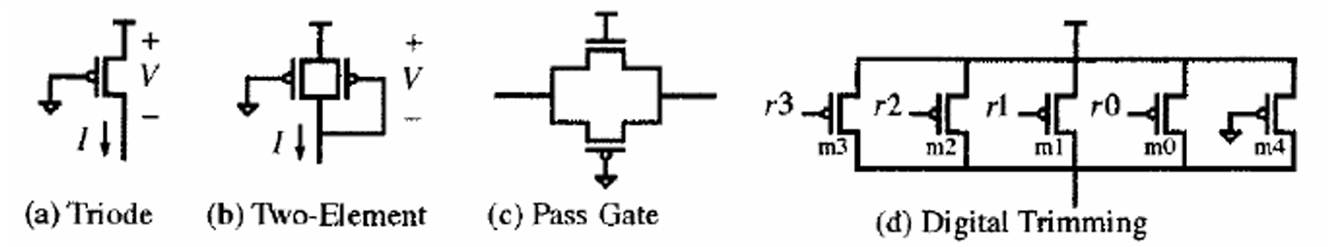
\includegraphics[width=0.9\linewidth]{img/TX_img/1)active_termination.png}
    \caption{Active termination}
    \label{fig:active_term}
\end{figure}

% --- Second Image: Combination ---
\begin{figure}[htbp]
    \centering
    
\includegraphics[width=0.4\linewidth]{2)combined_termination.png}
    \caption{Combination of Active and Passive}
    \label{fig:combined_term}
\end{figure}

\subsection{Equalization} \label{subsec:equalization}
\begin{itemize}
\item Equalization goal is to flatten the frequency response out to the Nyquist Frequency and remove time-domain ISI. TXs use pre-emphasis to shape their output spectrum (e.g., boosting high-frequency or de-emphasizing low-frequency content) , We usually use \textbf{de-emphasis} to not to increase Swing because we are limited by supply , EMI which will cause cross-talk , but at the cost of attenuated transmit signal

\item The number of taps and maximum tap weights determine allowable de-emphasis value and the quality of equalization both are usually specified by standards as more equalization , attenuates signal at small
frequency , so we limit this equalization because I have minimum eye opening

\item One approach to set the TX FIR coefficients is a \textbf{Minimum Mean-Square Error (MMSE) Algorithm}
\end{itemize}

\begin{figure}[htbp]
    \centering
    % 1. The Photo First
    
\includegraphics[width=0.5\textwidth]{3)Tx_FFE_Implementation.png}
    
    \vspace{10pt} 
    
    % 2. Mathematical representation exactly as requested
    \begin{center}
        \textbf{Low Frequency Response (Sum Taps)} \\
        $[\dots \enspace 1 \enspace 1 \enspace 1 \enspace \dots] * [-0.131 \enspace 0.595 \enspace -0.274] = [\dots \enspace 0.190 \enspace 0.190 \enspace 0.190 \enspace \dots]$ \\[10pt]
        \textbf{Nyquist Frequency Response (Sum Taps w/ Alternating Polarity)} \\
        $[\dots \enspace -1 \enspace 1 \enspace -1 \enspace \dots] * [-0.131 \enspace 0.595 \enspace -0.274] = [\dots \enspace 1 \enspace -1 \enspace 1 \enspace \dots]$
    \end{center}
    
    \vspace{5pt}
    
    % 3. The Caption at the very end
    \caption{Tx FFE Example}
    \label{fig:tx_ffe_example}
\end{figure}

\begin{figure}[H]
    \centering
    % --- Subfigure (a) ---
    \begin{subfigure}{0.32\textwidth}
        \centering
        
\includegraphics[width=\textwidth]{4.1)Channel_frequency_response.png}
        \caption{}
        \label{fig:channel_response}
    \end{subfigure}
    \hfill
    % --- Subfigure (b) ---
    \begin{subfigure}{0.32\textwidth}
        \centering
        
\includegraphics[width=\textwidth]{4.2)FIR_frequency_response.png}
        \caption{}
        \label{fig:fir_response}
    \end{subfigure}
    \hfill
    % --- Subfigure (c) ---
    \begin{subfigure}{0.32\textwidth}
        \centering
        
\includegraphics[width=\textwidth]{4.3)Combined_channel_and_Tx.png}
        \caption{}
        \label{fig:combined_response}
    \end{subfigure}

    \vspace{0.3cm}
    \caption{ (a) Channel frequency response ; (b) FIR frequency response ; (c) Combined channel and Tx}
    \label{fig:equalization_plots}
\end{figure}

\begin{figure}[H]
    \centering
    
\includegraphics[width=1\textwidth ]{5)sent_data.png}
    \caption{(a) Tx and Rx signals with lossy channel without Tx EQ; (b) Tx Pre-distorted output to compensate for channel ISI; (c) Rx received signal with Tx EQ}
    \label{fig:sent_data}
\end{figure}

\begin{itemize}
\item If no Tx pre-emphasis is used the single bit transitions are heavily attenuated compared to CIDs
\item When Tx pre-emphasis is used the transition bits are emphasized, non transition but are not emphasized
\item The channel attenuates the transition bits more than the non transition bits due to their higher frequency content
\item At the receiver input both transition and non transition bits have the same amplitude, i.e. ISI is eliminated
\end{itemize}

\begin{figure}[H]
    \centering
    
\includegraphics[width=1\textwidth ]{6)EYE.png}
    \caption{(a) RX eye diagram with lossy channel without Tx EQ; (b) Tx output eye diagram with pre-emphasis (pre-distorted eye); (c) Rx received eye diagram with Tx pre-emphasis}
    \label{fig:EYE}
\end{figure}

\begin{itemize}
\item Receiver eye was nearly closed without using Tx pre-emphasis resulting in high BER
\item After applying the right amount of pre-emphasis, ISI can be eliminated from the received eye
\item However, pre-emphasis also reduces the outer eye opening, i.e. the non 
transition bits are de-emphasized, thus a maximum limit is usually set by 
standards on how much pre-emphasis can be used

\end{itemize}
\newpage
\section{Analog-based and DAC-based Drivers} \label{sec:Analog/DAC-based}

The implementation of Feed-Forward Equalization (FFE) generally falls into two categories based on how the tap summation and signal modulation are performed.

\subsection{Analog-based transmitters} \label{subsec:Analog-based}
In analog-based transmitters, the equalization is performed by summing currents or voltages of the taps directly at the output node.

\begin{itemize}
    \item \textbf{Implementation Idea:} Tap weights are implemented by adjusting the number of active slices for each cursor (Pre, Main, and Post).
    \item \textbf{FFE Taps and Clocking:} To achieve UI-spaced FFE taps, custom digital delay elements such as latches are required. For tap programmability, high-speed MUXs clocked with multiple phases (half- or quarter-rate) are necessary. This significantly increases the complexity of the clocking tree and the capacitive load, often forcing equalization and tap selection to be handled at higher speeds.
    \item \textbf{Modulation Challenges:} Supporting higher modulation techniques, such as PAM-4, requires multiple serializers (e.g., separate paths for MSB and LSB) for a single cursor. This increases the capacitive loading on the transmitter output, which degrades the output bandwidth and significantly increases power consumption and complexity as the number of taps grows.
\end{itemize}


 \begin{figure}[htbp]
     \centering
     
\includegraphics[width=0.8\textwidth]{7)Analog-based}
     \caption{Analog-based Transmitter Architecture.}
 \end{figure}

\subsection{DAC-based transmitters} \label{subsec:DAC-based}
DAC-based transmitters move the equalization and tap weight calculation into the digital domain, using a Digital to Analog Converter (DAC) as the final output stage.
DAC-based architectures the dominant choice for TXs with five or more FFE taps

\begin{itemize}
    \item \textbf{Implementation Idea:} Equalization is performed digitally within a DSP. The DSP outputs a digital code representing the required analog voltage for each bit sent into the channel.
    \item \textbf{FFE Taps and Clocking:} Both the generation of taps and their programmability are handled in the digital domain. This eliminates the need for high-speed analog delay elements or high-speed MUXs for tap selection. Consequently, the pre-driver circuitry is much simpler, and the load on the clocking distribution is reduced , helping equalization and tap selection to be handled at lower speeds .
    \item \textbf{Modulation Flexibility:} The driver functions as a DAC that represents the weight of the bit code. This structure remains the same regardless of the modulation technique used. This architecture offers superior flexibility for supporting advanced modulation schemes like PAM-4 or PAM-8 without the massive complexity scaling seen in analog designs.
\end{itemize}


\begin{figure}[htbp]
     \centering
     
\includegraphics[width=0.8\textwidth]{8)DAC_Based}
     \caption{DAC-based Transmitter Architecture.}
 \end{figure}

 \subsubsection{Digital TX FFE} \label{ssubsec:DSP}

Digital TX FFEs are often implemented using Look-Up Tables (LUTs). A fully LUT-based implementation stores an $N$-tap filter span computation in an LUT, which requires an $N \cdot \log_2(M)$-bit address (for $M$-PAM modulation) and an output word width equal to the DAC resolution.

\begin{itemize}
    \item  For example, as shown in Fig.~\ref{fig:dac_ffe_lut_full}, a 2-PAM 4-tap FFE with 6-bit DAC resolution requires 16 rows and 6 columns, totaling 96 registers or memory cells. However, this architecture does not scale well for 4-PAM systems; a 7-tap FFE with 7-bit resolution would require $2^{14} \times 7 = 114,688$ registers.
    
    \item  Instead, a more efficient 4-PAM architecture, illustrated in Fig.~\ref{fig:dac_ffe_lut_per_tap}, uses per-tap LUTs to eliminate multipliers and employs digital adders to combine the tap values. This approach allows for simple 4-row LUTs per tap.
    
    \item Given the dramatic reduction in row count, the internal DSP resolution can be increased to 8 bits. This reduces quantization noise in the subsequent adders before the signal is finally quantized to the 7-bit DAC resolution.
    
    \item Using this per-tap approach, a 4-PAM 7-tap FFE can be implemented with only 224 registers ($7 \text{ taps} \times 4 \text{ rows} \times 8 \text{ bits}$), making it much more hardware-efficient.
\end{itemize}

\begin{figure}[htbp]
    \centering
    % --- Subfigure A ---
    \begin{subfigure}{0.35\textwidth} % Increased slightly for better visibility
        \centering
        
\includegraphics[width=\textwidth]{9)DAC_FFE_1.png}
        \caption{}
        \label{fig:dac_ffe_lut_full}
    \end{subfigure}
    \hfill % This pushes (a) to the left and (b) to the right
    % --- Subfigure B ---
    \begin{subfigure}{0.6\textwidth} % Adjusted to fill the remaining space
        \centering
        
\includegraphics[width=\textwidth]{9)DAC_FFE_2.png}
        \caption{}
        \label{fig:dac_ffe_lut_per_tap}
    \end{subfigure}
    
    \vspace{0.3cm}
    \caption{Digital TX FFE implementations. (a) Fully LUT-based 2-PAM 4-tap FFE with 6b output resolution; (b) 4-PAM 7-tap FFE with tap-based LUTs and 7b output resolution.}
    \label{fig:dac_ffe_comparison}
\end{figure}
The reduction in register count is driven by the mathematical difference between \textbf{exponential growth} and \textbf{linear growth} as the number of taps ($N$) increases.

In the standard approach, a 7-tap 4-PAM system must account for every possible input combination ($4^7 = 16,384$ combinations) and gives the output directly. By treating each tap independently (multiplying each tap with its tap weight), the per-tap approach only needs to store 4 possible values for each of the 7 taps.
\begin{table}[htbp]
    \centering
    \caption{Comparison of the 2 Implementation Architectures}
    \label{tab:lut_comparison}
    \begin{tabular}{@{}lll@{}}
        \toprule
        \textbf{Feature} & \textbf{Fully LUT-Based Approach} & \textbf{Per-Tap LUT Approach} \\ \midrule
        Logic Basis & $2^{N \cdot \log_2(M)}$ rows & $M$ rows per tap \\
        Scaling for 4-PAM 7-Tap & Requires $2^{14}$ addresses & Requires $4$ rows $\times 7$ taps \\
        Total Registers & 114,688 registers & 224 registers \\ \bottomrule
    \end{tabular}
\end{table}

\section{Driver Topologies} \label{sec:Driver_topologies}
\subsection{Voltage Mode} \label{subsec:Voltage_mode}
\subsubsection{NRZ SST} \label{ssubsec:NRZ_SST}

\begin{figure}[H]
    \centering
    % --- Subfigure (a) ---
    \begin{subfigure}{0.4\linewidth}
        \centering
        
\includegraphics[width=\textwidth]{10)SST}
        \caption{}
        \label{fig:SST}
    \end{subfigure}
    \hfill
    % --- Subfigure (b) ---
    \begin{subfigure}{0.21\linewidth}
        \centering
        
\includegraphics[width=\textwidth]{10.1)Equivalent_Circuit}
        \caption{}
        \label{fig:Equivalent Circuit_NRZ}
    \end{subfigure}
    \hfill
    \vspace{0.3cm}
    \caption{ (a) SST ; (b) Equivalent Circuit}
    \label{fig:NRZ SST}
\end{figure}

\begin{itemize}
    \item SST driver consists of inverters driving series termination resistors.
    \item Actual source impedance is a series combination of $R_{TERM}$ and $Z_{NMOS}$ or $Z_{PMOS}$.
    \item The series resistors provide ESD protection for transistors’ drain junctions.
    \item Transistor impedance varies with region of operation and PVT corners.
    \item Differential peak-to-peak output swing is equal to $V_{DD}$.
\end{itemize}


\subsubsection{PAM-4 SST} \label{ssubsec:PAM-4_SST}

\begin{figure}[H]
    \centering
    % --- Top Row ---
    \begin{subfigure}[t]{0.48\linewidth} % Adjusted to fit side-by-side
        \centering
        
\includegraphics[width=\textwidth]{11)PAM4_SST}
        \caption{2-bit (PAM-4) SST Architecture}
        \label{fig:PAM4_SST_Circuit}
    \end{subfigure}
    \hfill % Pushes subfigures to the edges
    \begin{subfigure}[t]{0.48\linewidth} % Adjusted to fit side-by-side
        \centering
        
\includegraphics[width=\textwidth]{11.2)Equivalent_Circuit_PAM4}
        \caption{Equivalent Circuit}
        \label{fig:Equivalent_Circuit_PAM4}
    \end{subfigure}

    \vspace{0.5cm} % Adds vertical space before the next row

    % --- Bottom Row (A blank line above this forces it down) ---
    \begin{subfigure}[t]{0.6\linewidth} % Larger width for the centered EYE
        \centering
        
\includegraphics[width=\textwidth]{11.3)EYE}
        \caption{EYE Diagram}
        \label{fig:sttpam4eye}
    \end{subfigure}
    
    \caption{}
    \label{fig:PAM-4_SST_Main}
\end{figure}


\begin{itemize}
\item It can be Considered as a 2 bit DAC corresponding to 3 identical slices ($2^{n}-1$) 
\item So We want to make the resistance of all the parallel slices gives 50$\Omega$ so the resistance of one slice = 50X3 $\Omega$ and Width of each slice = 3*W wanted where the whole driver will have Width = W and R=50$\Omega$
\item Voltage divider is made for each input and for complementary input : the 2 terminals of Vout are swapped so for Vppd it will be the same with opposite sign
\end{itemize}
\newpage

\subsection{Current Mode} \label{subsec:Current_mode}
\subsubsection{NRZ CML} \label{ssubsec:NRZ_CML}
 \begin{figure}[H]
     \centering
     
\includegraphics[width=0.8\textwidth]{12)CML}
     \caption{Conventional CML.}
 \end{figure}
 \begin{itemize}
    \item Differential pair steers the current into a differential I/O link.
    \item Differential pp RX swing is \textbf{$\pm IR/2$.}
    \item Note that \textbf{Swing = IR} and \textbf{Vo,CM = VDD-IR/2}, so by ignoring supply variations, we can have precise Swing and CM by using I outputted from Bandgap which track $1/R$ and use poly resistor so If R shifted I will shift opposite to it So swing and CM become constant.
    \item For high swing (Large current) we will need large i/p pair to have lower $V_{GS}$ and preserve current source in Sat. For ex: $0.8V_{pp}$ swing needs $I_B=16mA$ (w/o taking current mirrors into considerations).
    \item So a pre-driver is necessary to drive the large capacitance of the output stage (chain of inverters).
    \item Tradeoffs between Power, speed, swing, BER.
\end{itemize}


\clearpage
\subsubsection{PAM-4 CML} \label{ssubsec:PAM-4_CML}
\begin{figure}[H]
    \centering
    % --- Top Row ---
    \begin{subfigure}[t]{0.48\linewidth} % Adjusted to fit side-by-side
        \centering
        
\includegraphics[width=\textwidth]{13)PAM4CML}
        \caption{2-bit (PAM-4) CML Architecture}
        \label{fig:PAM4_SST_Circuit}
    \end{subfigure}
    \hfill % Pushes subfigures to the edges
    \begin{subfigure}[t]{0.51\linewidth} % Adjusted to fit side-by-side
        \centering
        
\includegraphics[width=\textwidth]{13.1)Equiv_cir}
        \caption{Equivalent Circuit}
        \label{fig:Equivalent_Circuit_PAM4}
    \end{subfigure}

    \vspace{0.5cm} % Adds vertical space before the next row

    % --- Bottom Row (A blank line above this forces it down) ---
    \begin{subfigure}[t]{0.5\linewidth} % Larger width for the centered EYE
        \centering
        
\includegraphics[width=\textwidth]{13.2)EYE}
        \caption{EYE Diagram}
        \label{fig:sttpam4eye}
    \end{subfigure}
    
    \caption{}
    \label{fig:PAM-4_SST_Main}
\end{figure}
\noindent \textbf{For D<1:0>=10:} 

\begin{enumerate}
    \item \textbf{KCL at node $V_{on}$}:
    \begin{equation}
        \frac{V_{DD} - V_{on}}{R} + I_{2R} = \frac{2}{3}I \label{eq:kclnodevon10}
    \end{equation}
    
    \item \textbf{KCL at node $V_{op}$}:
    \begin{equation}
        \frac{V_{DD} - V_{op}}{R} - I_{2R} = \frac{1}{3}I \label{eq:kclnodevop10}
    \end{equation}
\end{enumerate}

Subtracting equation \eqref{eq:kclnodevop10} from equation \eqref{eq:kclnodevon10} yields:
\begin{equation}
    \frac{V_{op} - V_{on}}{R} + 2I_{2R} = \frac{1}{3}I
    \label{eq:substpam4cml}
\end{equation}

By Ohm's Law, the differential voltage is defined as $V_{op} - V_{on} = I_{2R}(2R)$ . Substituting this into equation \eqref{eq:substpam4cml}:
\begin{equation}
    \frac{2R \cdot I_{2R}}{R} + 2I_{2R} = \frac{1}{3}I
\end{equation}

\begin{equation}
    4I_{2R} = \frac{1}{3}I \implies I_{2R} = \frac{1}{12}I
\end{equation}

This result confirms that the current passing through the bridging resistor is exactly $1/12$ of the total tail current $I$ 
\begin{equation}
    V_{diff} = +\frac{1}{12}I \times 2R = +\frac{1}{6}IR 
     \label{eq:vout_final}
\end{equation}
\begin{align}
    V_{oN} &= V_{DD} - \frac{7}{12} IR \\
    V_{oP} &= V_{DD} - \frac{5}{12} IR
\end{align}
And for the Complementary input , for differential peak to peak , We know that it is just change in the direction of the current so Vppd is the same with opposite sign
\noindent \textbf{For D<1:0>=11:} 


\begin{equation}
    I_{2R} = \frac{1}{4}I_s
\end{equation}

The differential output voltage $V_{diff}$ is then calculated as:
\begin{equation}
    V_{diff} = I_{2R}(2R) = \left( \frac{1}{4}I_s \right)(2R) = \frac{1}{2}I_sR
\end{equation}
\begin{align}
    V_{oN} &= V_{DD} - \frac{3}{4} IR \\
    V_{oP} &= V_{DD} - \frac{1}{4} IR
\end{align}
\newpage
\subsubsection{H-bridge CML} \label{ssubsec:H_CML}

 \begin{figure}[H]
     \centering
     
\includegraphics[width=0.5\textwidth]{14)H-bridge}
     \caption{H-Bridge}
 \end{figure}
 \begin{itemize}
    \item \textbf{Output Swing Calculation}:  $V_{oPP,diff} = 2I_B R$ .
    \item \textbf{Power and Area Trade-offs}: Swing is doubled for the same power consumption but requires a larger circuit area . For the same swing as CML, we need $1/2$ the size of the NMOS input pair, but the addition of PMOS transistors with sizes larger than $1/2$ the area of the CML NMOS increases parasitic capacitance .
    \item \textbf{Headroom and Common-Mode (CM) Challenges}: The presence of two series current sources occupies a large voltage headroom . Furthermore, the output CM is not inherently defined; this can be resolved using a CMFB (Common-Mode Feedback) loop or by implementing a hybrid topology .
    \item \textbf{Hybrid Topology}: In a hybrid configuration, the SST defines the output CM, and the CML adds its swing on top of it; however, this approach increases self-loading .
\end{itemize}

\subsubsection{Tailless} \label{ssubsec:Tailless}
 \begin{figure}[H]
     \centering
     
\includegraphics[width=1\textwidth]{16)Tailless}
     \caption{Tailless}
 \end{figure}
The tailless driver architecture offers significant advantages for high-speed data transmission by optimizing the transistor biasing and reducing parasitic effects.

\begin{itemize}
    \item \textbf{Device Operation}: The tailless driver consists of switching and cascode transistors that are flipped from the input and tail current source used in standard CML drivers. This configuration requires only the cascode (Casc) devices to remain in the saturation region for proper operation and they are whom defines current and though swing.
    
    \item \textbf{Parasitic Reduction}: By eliminating the tail current source, the $V_{GS}$ of the input pair can be increased. This allows the driver to deliver the same current (and thus the same output swing) using a smaller input pair, which significantly decreases parasitic capacitance. However, a high overdrive voltage ($V_{OV}$) must be managed to prevent transistors from entering the linear region.
    
    \item \textbf{Device Protection}: The $V_{DS}$ of the switches is determined by the $V_{GS}$ of the cascode transistors. Applying an appropriate $V_{casc}$ protects the input transistors from large output swings, enabling the use of thin-oxide devices which are essential for achieving the final high data rate.
    
    \item \textbf{Current Control}: In specific configurations, the P1 in fig(b) can disable current flow in the driver by pulling the source of N1 to the supply voltage when the digital input ($DIN$) is low.
    
    \item \textbf{Output Impedance ($R_{out}$)}: The cascode transistors are the primary devices forcing current, typically requiring a high channel length ($L$). However, since they connect directly to the output, $L$ is kept small to avoid increasing parasitics. To compensate and boost $R_{out}$, a "super $g_m$" configuration is  in fig(c), which is further amplified by the loop gain ($LG$).
\end{itemize}

\subsection{Hybrid Mode} \label{subsec:Hybrid_mode}
\begin{itemize}
    \item Since V.mode max swing is VDD and CML high swings will give high non linearity , Hybrid topology is proposed to make the best compromise of them in addition to increasing the output swing above VDD
    \item For the corner @which supply decrease -10\% and 50mV routing so supply is 670mV , we will want 130mV additional swing from the CML to acheive the standard swing spec specified in table \ref{tab:pcie6_tx_specs_full} , so we will give margin and say we want 135mV swing
\end{itemize}

\subsubsection{NRZ NMOS CML}
\begin{figure}[H]
    \centering
    \begin{subfigure}{0.5\linewidth} % Use linewidth for the environment
        \centering
        
\includegraphics[width=\textwidth]{17.1)Hybrid_NMOS_CML}
        \caption{}
    \end{subfigure}
    \hfill
    \begin{subfigure}{0.6\linewidth} % Use linewidth for the environment
        \centering
        
\includegraphics[width=\textwidth]{17.1)Hybrid_NMOS_CML_EQ_CIRC}
        \caption{}
    \end{subfigure}
    \caption{(a) NRZ NMOS CML; (b) Equivalent Circuit.}
\end{figure}
\begin{itemize}
    \item The current distribution is only made by for I bas and VDD is deactivated (superposition) 
    \item This topology will give Vppd = VDD+IR
    \item It is obvious that this topology isn't suitable as VDS on Current source and Input is too low
    \item  Assuming for the corner that the supply is low (670mV) and we want IR=135mV so VoutP = 66.25mV which is bad headroom
\end{itemize}
 
\subsubsection{NRZ PMOS CML}
\begin{figure}[H]
    \centering
    \begin{subfigure}{0.5\linewidth} % Use linewidth for the environment
        \centering
        
\includegraphics[width=\textwidth]{17.2)Hybrid_PMOS_CML}
        \caption{}
    \end{subfigure}
    \hfill
    \begin{subfigure}{0.6\linewidth} % Use linewidth for the environment
        \centering
        
\includegraphics[width=\textwidth]{17.2)Hybrid_PMOS_CML_EQ_CIRC}
        \caption{}
    \end{subfigure}
    \caption{(a) NRZ PMOS CML; (b) Equivalent Circuit.}
\end{figure}
\begin{itemize}
    \item This topology will give Vppd = VDD+IR
    \item Same VDS as the prev topology and it is still unsuitable

\end{itemize}
\newpage
\subsubsection{NRZ H-bridge CML}
\begin{figure}[H]
    \centering
    \begin{subfigure}{0.5\linewidth} % Use linewidth for the environment
        \centering
        
\includegraphics[width=\textwidth]{17.3)Hybrid_HBridge_CML}
        \caption{}
    \end{subfigure}
    \hfill
    \begin{subfigure}{0.6\linewidth} % Use linewidth for the environment
        \centering
        
\includegraphics[width=\textwidth]{17.3)Hybrid_HBridge_CML_EQ_CIRC}
        \caption{}
        \label{fig:NRZ_HBRIDGECMLEQCIRC}
    \end{subfigure}
    \caption{(a) NRZ H-Bridge CML; (b) Equivalent Circuit.}
\end{figure}
\begin{itemize}
    \item This topology will give Vppd = VDD+2IR as the H-bridge topology made 1/2 of I bias pass through RX termination instead of 1/4Ibias
    \item It will give VDS = 133.75mV which is more suitable than the prev topologies but note that input pair will be in triode (|VG-VD| $\approx$ 666.25mV >|VTH| so this should be considered in Resistance calibration)

\end{itemize}
\newpage
\subsubsection{PAM-4 H-bridge CML}

\begin{figure}[H]
    \centering
    \begin{subfigure}{0.6\linewidth} % Use linewidth for the environment
        \centering
        
\includegraphics[width=\textwidth]{17)Hybrid}
        \caption{}
    \end{subfigure}
    \hfill
    \begin{subfigure}{0.7\linewidth} % Use linewidth for the environment
        \centering
        
\includegraphics[width=\textwidth]{17)HybridPAM4EQCIRC.png}
        \caption{}
        \label{}
    \end{subfigure}
    \caption{(a) Hybrid H-bridge Driver; (b) Equivalent Circuit for D<1:0> = 10.}
\end{figure}
\begin{itemize}
    \item For $D\langle 1:0 \rangle = 11, 00$: \newline 
    The equivalent circuit is the same as fig \ref{fig:NRZ_HBRIDGECMLEQCIRC} and 
    $\bm{V_{ppd} = V_{DD} + 2RI = V_{DD} + \Delta V}$
\item For $D\langle 1:0 \rangle = 10, 01$:
\begin{align*}
    % Top line: Entire equation is bold, but "where" is standard weight
    \pmb{V_{ppd}} &\pmb{= \frac{V_{DD}}{3} + \frac{2RI}{3} = \frac{V_{DD}}{3} + \frac{\Delta V}{3},} \quad \text{where } \pmb{\Delta I = \frac{I}{3}} \\
    % Lower lines: Return to standard weight
    V_{DS(I_{LSB})} &= \frac{7}{12} V_{DD} + \frac{1}{2} R \Delta I = 509.6 \text{ mV} \\
    V_{DS(I_{MSB})} &= \frac{5}{12} V_{DD} - \frac{1}{2} R \Delta I = 269 \text{ mV}
\end{align*}


\end{itemize}
\subsection{Comparisons} \label{subsec:comp}
\subsubsection{Power} \label{ssubsec:Power}
\begin{figure}[H]
     \centering
     
\includegraphics[width=0.7\textwidth]{18.1)powercml}
     \caption{}
 \end{figure}
 \begin{figure}[H]
     \centering
     
\includegraphics[width=0.7\textwidth]{18.2)powersst}
     \caption{}
 \end{figure}
 \clearpage
 
 \subsubsection{Swing} \label{ssubsec:Swing}
\begin{figure}[H]
    \centering
    % --- Subfigure A ---
    \begin{subfigure}{0.65\textwidth} % Increased slightly for better visibility
        \centering
        
\includegraphics[width=\textwidth]{15)comp1}
        \caption{}
        \label{}
    \end{subfigure}
    \hfill % This pushes (a) to the left and (b) to the right
    % --- Subfigure B ---
    \begin{subfigure}{0.6\textwidth} % Adjusted to fill the remaining space
        \centering
        
\includegraphics[width=\textwidth]{15)comp2}
        \caption{}
        \label{}
    \end{subfigure}
    
    \vspace{0.3cm}
    \caption{CML Swings for SE termination. (a) CML; (b) H-bridge.}
    \label{fig:dac_ffe_comparison}
\end{figure}
\noindent \textbf{For CML : }
Total current is passing in one branch
\noindent \textbf{For H-Bridge :}
Total Current is passing in each of the 2 branches
• Current is divided equally between TX termination and RX termination
• ½  of the current reached to each SE  termination of the receiver
\begin{figure}[H]
    \centering
    % --- Subfigure A ---
    \begin{subfigure}{0.65\textwidth} % Increased slightly for better visibility
        \centering
        
\includegraphics[width=\textwidth]{15)comp3}
        \caption{}
        \label{}
    \end{subfigure}
    \hfill % This pushes (a) to the left and (b) to the right
    % --- Subfigure B ---
    \begin{subfigure}{0.65\textwidth} % Adjusted to fill the remaining space
        \centering
        
\includegraphics[width=\textwidth]{15)comp4}
        \caption{}
        \label{}
    \end{subfigure}
    
    \vspace{0.3cm}
    \caption{CML Swings for Differential termination. (a) CML; (b) H-bridge.}
    \label{}
\end{figure}

\noindent \textbf{For CML : }
\begin{itemize}
    \item at D=VDD , Db=0 :
    \begin{align}
        V_1 &= V_{DD} - \frac{3}{4} I_b R_T \\
        V_2 &= V_{DD} - \frac{1}{4} I_b R_T
    \end{align}
    \item ¼ of the current reached the differential Termination of the receiver
    \item The 2nd termination of TX became series with RX termination
\end{itemize}
\noindent \textbf{For H-Bridge :}
Total Current is passing in each of the 2 branches
• Current is divided equally between TX termination and RX termination
• ½  of the current reached the differential Termination of the receiver
 \begin{figure}[H]
     \centering
     
\includegraphics[width=1\linewidth]{10.2)Swings}
     \caption{ SST Swings a) SE Termination ; b) Differential Termination}
 \end{figure}
 
\noindent \textbf{For SE termination:}
\begin{align}
    V_{d,1} &= (Vs/2) & V_{d,0} &= -(Vs/2) \\
    V_{d,pp} &= Vs & I &= \frac{V_{d,pp}}{2R}              
\end{align}

\vspace{0.5cm}

\noindent \textbf{For Differential termination:}
\begin{align}
    V_{d,1} &= (Vs/2) & V_{d,0} &= -(Vs/2) \\
    V_{d,pp} &= Vs & I &= \frac{V_{d,pp}}{4R}     
\end{align}
\clearpage
 \subsubsection{Summary} \label{ssubsec:Summary}
\begin{table}[htbp]
    \centering
    \caption{Comparison Between Current Mode and Voltage Mode Driver Topologies}
    \label{tab:driver_comparison}
    \begin{tabularx}{\textwidth}{l X X}
        \toprule
        \textbf{Feature} & \textbf{Current Mode} & \textbf{Voltage Mode} \\
        \midrule
        \textbf{Swing} & Swing is set by current . & Swing is set by Supply. \\
        \addlinespace
        \textbf{Termination} & termination is set by $Z_0$ at high $R_{out}$. &  termination set by $Z_0$ and devices. \\
        \addlinespace
        \textbf{Power} & Static power; Less power efficient for same swing. & Dynamic power;  but for high speed , the very fast transitions can be averaged to be compared with static current,  more power efficient for same swing. \\
        \addlinespace
        \textbf{Speed} & faster due to constant current source activation  &  it is slower as it depends on charging and discharging caps \\        

        \addlinespace
        \textbf{SSO} & Static steered current prevents fast transitions. & Fast transitions can lead to supply bounce if parasitic inductors are present. \\
        \addlinespace
        \textbf{Programmability} & Swing is analog-programmed via current source without altering driver impedance. & Harder termination controllability ($R_{ON}$ depends on $\mu, V_{th}$, etc.). Analog Tuning through header/footer CSs degrades linearity. \\
        \addlinespace
        \textbf{Linearity} & Degraded linearity as current source operates in different regions during transitions. & Better linearity; series resistance overcomes $R_{ON}$ non-linearity. \\
        \addlinespace
        \textbf{Trade-offs} & Swing $\uparrow$, $V_{oCM} \downarrow$, headroom $\downarrow$, linearity $\downarrow$ (tail operates close to triode). Input size $\uparrow$, headroom for tail $\uparrow$, BW $\downarrow$. & Linearity vs. Speed trade-off. Increasing $Z_0/R_{ON}$ improves linearity but degrades bandwidth (BW). \\
        \bottomrule
    \end{tabularx}
\end{table}
 
\newpage


\chapter{Clocking Network Implementation}
\lhead{Chapter 2. \emph{implementation}}
\section{I/Q Divider}

The IQ Divider is the primary frequency-translation element in the transmitter clocking path, responsible for converting the high-frequency PLL output into multiple phases at a lower fundamental frequency.

\subsection{Architecture and Operation}
The most common implementation for generating precise quadrature phases at high frequencies is a \textbf{Divide-by-2 circuit} composed of two cascaded differential static latches (Master and Slave) configured in a negative feedback loop.

\begin{itemize}
    \item \textbf{Master-Slave Configuration:} The two latches are connected in series, with the output of the slave latch cross-coupled and fed back to the input of the master latch.
    
    \item \textbf{Clocking:} The differential 16 GHz clock from the PLL drives the clock inputs of the latches in opposite phases.
    
    \item \textbf{Quadrature Generation:} Because the latches trigger on opposite edges of the high-speed clock, the master latch output is shifted by $90^\circ$ relative to the slave latch output. This produces the four fundamental quadrature phases ($0^\circ, 90^\circ, 180^\circ, 270^\circ$) at an 8 GHz frequency.
    
    \item \textbf{Static vs. Dynamic:} Static latches are preferred in many designs for their robustness across a wide frequency range and better tolerance to process variations compared to dynamic logic.
\end{itemize}

\begin{figure}[H]
    \centering
    
\includegraphics[width=0.8\textwidth]{IQ.jpg}
    \caption{Divider as a master–slave arrangement of two latches. IN+/IN- are the differential input signals, while OUTI+/OUTI- and OUTQ+/OUTQ- are the two quadrature differential output signals.}
    \label{fig:Wire Scaling}
\end{figure}


\subsection{Topology Selection}
The choice of a clocked tri-state inverter-based latch over alternative structures like Current Mode Logic (CML) or dynamic logic is driven by several design requirements:

\begin{itemize}
    \item \textbf{Full-Swing Operation:} The tri-state inverter provides rail-to-rail output levels, ensuring high noise immunity and eliminating the need for additional level shifters before the pulse-shaping stage.
    \item \textbf{Dynamic Power Scaling:} Power consumption is primarily dynamic, allowing for better efficiency in quarter-rate architectures where the distribution frequency is reduced to 8 GHz.
    \item \textbf{PVT Robustness:} As a static implementation, it avoids the leakage and charge-sharing issues inherent in dynamic topologies, providing a stable $90^\circ$ phase relationship across all operating corners.
\end{itemize}

\begin{figure}[H]
    \centering
    
\includegraphics[width=0.7\textwidth]{c2mos.jpg}
    \caption{Clocked CMOS ($C^2MOS$).}
    \label{fig:Wire Scaling}
\end{figure}


\subsection{Negative Latch Schematic (Clocked $C^2$MOS)}
\label{subsec:negative_latch_sim}

The fundamental building block of the IQ divider is the differential static latch, implemented here using a \textbf{Clocked CMOS ($C^2$MOS)} topology. This structure is chosen for its high-speed performance and rail-to-rail output swing.

\begin{itemize}
    \item \textbf{Input Stage:} The schematic features a clocked tri-state inverter where the input signal is gated by the differential clock signals ($\text{CLK}$ and $\text{CLKb}$). This ensures that the input is only sampled during the active phase of the clock.
    
    \item \textbf{Storage Element:} A cross-coupled inverter pair (regenerative latch) is utilized to maintain the logic state when the input stage enters a high-impedance (tri-state) mode.
    
    \item \textbf{Operation:} When the clock is active, the tri-state inverter is enabled, and the latch transparently passes the input to the output. When the clock toggles, the input stage disconnects, and the cross-coupled structure holds the previous value, providing robust static operation and immunity to leakage.
\end{itemize}

\begin{figure}[H]
    \centering
    
\includegraphics[width=1\textwidth]{N_latch.png}
    \caption{Negative Static Latch Schematic.}
    \label{fig:Wire Scaling}
\end{figure}

\subsection{IQ Divider System Schematic}
\label{subsec:iq_divider_system_sim}

The complete IQ divider is formed by cascading two of the previously described latches (Master and Slave) in a closed-loop configuration.

\begin{itemize}
    \item \textbf{Negative Feedback Loop:} The differential outputs of the slave latch are cross-coupled and fed back to the inputs of the master latch. This inversion in the feedback path is what enables the frequency division (divide-by-2) functionality.
    
    \item \textbf{Quadrature Phase Generation:} 
    \begin{itemize}
        \item The Master Latch triggers on the rising edge of the clock.
        \item The Slave Latch triggers on the falling edge of the clock.
        \item This $180^\circ$ difference in the high-speed clock domain results in a precise $90^\circ$ phase shift at the divided output frequency, producing the $I$ and $Q$ phases ($0^\circ, 90^\circ, 180^\circ, 270^\circ$).
    \end{itemize}
    
    \item \textbf{Simulation Setup:} The schematic is simulated with a 16 GHz differential input clock to verify the generation of stable 8 GHz quadrature outputs.
\end{itemize}

\begin{figure}[H]
    \centering
    
\includegraphics[width=1\textwidth]{IQ_divider.png}
    \caption{I/Q Divider Schematic.}
    \label{fig:Wire Scaling}
\end{figure}

\subsection{Transient Response Analysis}
\label{subsec:transient_analysis}

The transient simulation results verify the functional operation of the IQ divider, specifically its ability to perform frequency division and generate accurate quadrature phases.

\begin{itemize}
    \item \textbf{Frequency Division and Scaling:} The top two traces show the differential input clocks ($CLK$ and $CLKb$) operating at the high-speed PLL\ frequency of 16~GHz. The four output traces ($C4\_0$ through $C4\_270$) operate at exactly half that frequency (8~GHz), confirming the successful divide-by-2 operation required for a quarter-rate clocking system.
    
    \item \textbf{Quadrature Phase Generation:} The simulation confirms the $90^\circ$ phase relationship between the outputs. By observing the simulation markers, it is evident that the $90^\circ$ phase ($C4\_90$) is shifted by half a clock cycle of the 16~GHz input relative to the $0^\circ$ phase ($C4\_0$). This equates to exactly one-quarter of the 8~GHz output period ($T/4$).
    
    \item \textbf{Timing Accuracy:} The crossing points of the quadrature phases align precisely with the 400~mV common-mode level (indicated by horizontal markers H1, H2, H3, and H4). The symmetry observed in the rising and falling edges indicates low internal Duty Cycle Distortion (DCD) within the divider circuit itself.
\end{itemize}

\begin{figure}[H]
    \centering
    
\includegraphics[width=1\textwidth]{Transient.png}
    \caption{Transient simulation waveforms of the IQ Divider showing the 16~GHz input clock and the generated 8~GHz quadrature phases ($I/Q$).}
    \label{fig:Wire Scaling}
\end{figure}

\subsubsection{Initialization and Metastability Resolution}

While the clocked $C^2$MOS topology provides robust static operation, the initial transient simulation revealed a severe startup vulnerability. Because the cross-coupled inverters in the master and slave latches are geometrically symmetrical, the divider is susceptible to metastability during power-up.

\begin{itemize}
    \item \textbf{The Metastability Problem:} If the internal nodes power up at or near the common-mode voltage (approximately 400 mV), the loop gain of the cross-coupled pair is perfectly balanced. As shown in the initial transient response, the circuit lingers in a metastable, mid-rail state for nearly 200 ns before thermal noise or minor asymmetric leakage finally pushes the latches into a valid logic state. In a multi-gigahertz transceiver system, this indeterminate startup delay could be unacceptable and can lead to severe synchronization failures downstream.
\end{itemize}

\begin{figure}[H]
    \centering
    
\includegraphics[width=1\textwidth]{metastability problem.png}
    \caption{Initial transient simulation showing the outputs lingering in a metastable mid-rail state before oscillating.}
    \label{fig:metastability_problem}
    \label{fig:Wire Scaling}
\end{figure}

\begin{itemize}
    \item \textbf{Schematic Modification:} To break this perfectly balanced loop and force a deterministic startup, an asynchronous reset mechanism was introduced to the latch schematic. Dedicated pull-up and pull-down transistors were added to the internal storage nodes, driven by complementary \texttt{Reset} and \texttt{Resetb} signals. 
\end{itemize}

\begin{figure}[H]
    \centering
    
\includegraphics[width=1\textwidth]{modified iq divider.png}
    \caption{Modified $C^2$MOS latch schematic incorporating asynchronous Reset/Resetb transistors to force a known initial state.}
    \label{fig:modified_iq_divider}
\end{figure}

\begin{itemize}
    \item \textbf{Resolved Transient Response:} When the reset signal is briefly asserted during the initial power-up phase, these auxiliary transistors overpower the cross-coupled pair, forcefully pulling the internal nodes to definitively high and low states. As demonstrated in the modified simulation results, the metastability dead-zone is completely eliminated. The 8 GHz quadrature phases ($0^\circ, 90^\circ, 180^\circ, 270^\circ$) begin toggling immediately and cleanly from $t = 0$, ensuring reliable and deterministic operation.
\end{itemize}

\begin{figure}[H]
    \centering
    
\includegraphics[width=1\textwidth]{modified iq results.png}
    \caption{Resolved transient response showing immediate and clean generation of the 8 GHz quadrature phases with no metastable delay.}
    \label{fig:modified_iq_results}
\end{figure}

\section{Pulse Generation: Symmetric AND Gate}

Following the frequency translation in the I/Q Divider, the 8~GHz quadrature clocks possess a 50\% duty cycle. However, high-speed multiplexing architectures we took was the Quadrature-Rate which will require four non-overlapping clocks for the high speed serialization process. To achieve the target 25\% duty cycle required for the subsequent multiplexing stages, a dedicated pulse generation block is implemented.

\subsection{Phase Overlap and Duty Cycle Conversion}

The fundamental mechanism for generating the 25\% duty cycle clock is the logical AND operation of two adjacent quadrature phases. As shown in the system-level schematic, the $0^\circ$ phase (\texttt{C4\_0}) and the $90^\circ$ phase (\texttt{C4\_90}) are fed into a 2-input AND gate. 

Because the $90^\circ$ phase is delayed by exactly one-quarter of the clock period relative to the $0^\circ$ phase, the two signals only overlap at a logic HIGH state for $T/4$. Consequently, the output of the AND gate (\texttt{C0\_25\%}) is a precise 8~GHz pulse train with a 25\% duty cycle. The schematic is simulated with a 20~fF load capacitor to accurately model the input capacitance of the succeeding driver stage.

\begin{figure}[H]
    \centering
    
\includegraphics[width=0.8\textwidth]{and2 schematic.png}
    \caption{Symbol-level schematic of the pulse generator, demonstrating the logical AND of $0^\circ$ and $90^\circ$ phases to synthesize a 25\% duty cycle output (\texttt{C0\_25\%}) driving a 20~fF load.}
    \label{fig:and2_schematic}
\end{figure}

\subsection{Transistor-Level Implementation (Symmetric Topology)}

In standard digital standard-cell libraries, a NAND gate utilizes an asymmetric pull-down network consisting of a single series NMOS stack. At multi-gigahertz frequencies, this asymmetry is highly problematic. Depending on which input arrives last (the top transistor or the bottom transistor), the internal node capacitances discharge differently, leading to varying propagation delays. This data-dependent delay manifests directly as deterministic jitter.

To ensure pristine timing accuracy for the 25\% duty cycle pulse, a \textbf{Symmetric AND Gate} topology was designed. 

\begin{itemize}
    \item \textbf{Dual-Stack Pull-Down Network:} The conventional single NMOS stack is replaced by two parallel series stacks (\texttt{N0}-\texttt{N1} and \texttt{N56}-\texttt{N2}). The gate connections are swapped between the two branches (IN1/IN2 on the left, IN2/IN1 on the right). This guarantees that regardless of which clock phase transitions last, the equivalent resistance and capacitive discharge path to ground remain perfectly identical, eliminating input-dependent skew.
    \item \textbf{Pull-Up Network:} The PMOS pull-up network (\texttt{P0}, \texttt{P52}) operates in parallel, inherently maintaining symmetric charging characteristics.
    \item \textbf{Output Buffering:} The symmetric NAND structure is followed by a high-speed inverter (\texttt{P8}, \texttt{N8}) to restore the signal polarity to a logical AND function and to provide the necessary drive strength to push the high-frequency pulses into the 20~fF load.
\end{itemize}

\begin{figure}[H]
    \centering
    
\includegraphics[width=1\textwidth]{and2 transistor level.png}
    \caption{Transistor-level schematic of the Symmetric AND Gate, featuring a dual-stack NMOS pull-down network to eliminate input-dependent propagation delay and minimize deterministic jitter.}
    \label{fig:and2_transistor}
\end{figure}

\subsection{Transient Simulation and Verification}

To verify the functionality of the pulse generation stage and its ability to drive realistic downstream loads, a transient simulation was performed. By replicating the symmetric AND gate across all adjacent quadrature pairs ($0^\circ \text{ AND } 90^\circ$, $90^\circ \text{ AND } 180^\circ$, $180^\circ \text{ AND } 270^\circ$, $270^\circ \text{ AND } 0^\circ$), a complete set of four staggered quarter-rate clocks was synthesized.

The simulation results exhibit the following critical performance metrics:

\begin{itemize}
    \item \textbf{Precise 25\% Duty Cycle:} The waveforms for \texttt{C0\_25\%} through \texttt{C3\_25\%} clearly demonstrate an active HIGH duration of exactly one-quarter of the clock period ($T/4$), with the signal remaining strictly LOW for the remaining $3T/4$.
    \item \textbf{Non-Overlapping Phasing:} A fundamental requirement for high-speed multiplexing is the prevention of simultaneous conduction between parallel data paths. The transient plot confirms that as one phase completely transitions to a logic LOW, the subsequent phase begins its rising edge. This strict non-overlapping relationship guarantees contention-free data serialization in the subsequent driver stages.
    
\end{itemize}

\begin{figure}[H]
    \centering
    
\includegraphics[width=1\textwidth]{and2 simulation results.png}
    \caption{Transient simulation demonstrating the generation of four robust, non-overlapping 25\% duty cycle clock phases (\texttt{C0\_25\%} to \texttt{C3\_25\%}) operating at 8~GHz.}
    \label{fig:and2_transient_results}
\end{figure}


\section{Duty Cycle Correction and Buffering Chain}

Following the synthesis of the quarter-rate clock, the signal must be distributed to the high-speed multiplexing stages. Maintaining signal integrity along this path is critical, requiring both active duty cycle management and an optimally sized buffer chain to drive the massive capacitive load of the multiplexer.



\subsection{Input Capacitance Extraction: Transient Method}

Before the clock can drive the 4:1 Serializer (MUX), an intermediate buffer chain is required. Designing an optimal Fanout-of-4 (FO4) buffer chain requires exact knowledge of both the load capacitance ($C_{load}$) of the 4:1 MUX and the input capacitance ($C_{in}$) of the first-stage unit inverter.

Because standard PDK models do not directly expose the massive nonlinear gate capacitances operating at 8~GHz, the capacitance was extracted using a \textbf{Transient Integration Method}. The fundamental relationship between charge ($Q$), capacitance ($C$), and voltage ($V$) is:

$$Q = CV \implies C = \frac{\Delta Q}{\Delta V}$$

By expressing charge as the integral of current over time, the capacitance can be accurately measured by simulating the transient current spike required to charge the transistor gates from 0~V to VDD (0.8~V):

$$C \approx \frac{\int I \, dt}{0.8}$$

\begin{figure}[H]
    \centering
    
\includegraphics[width=0.8\textwidth]{transient method.png}
    \caption{Testbench schematic for transient capacitance extraction, isolating the input stage of the 4:1 MUX.}
    \label{fig:transient_method_schematic}
\end{figure}

\begin{figure}[H]
    \centering
    
\includegraphics[width=1\textwidth]{transient current.png}
    \caption{Transient current spikes observed during the charging and discharging of the input gate capacitance. The area under the positive spike ($\int I \, dt$) represents the total injected charge.}
    \label{fig:transient_current_waveform}
\end{figure}

Using the Virtuoso Calculator to integrate the transient current pulse and dividing by the 0.8~V swing, the input capacitance of the 4:1 MUX was extracted as \textbf{197.9 fF} ($\approx$ 200 fF). Applying the identical methodology to a minimum-sized unit inverter yielded a base input capacitance of \textbf{0.681 fF}.

\begin{figure}[H]
    \centering
    
\includegraphics[width=0.7\textwidth]{input cap OF FOUR TO ONE MUX.png}
    \caption{Calculator evaluation of the transient integral, yielding a MUX input capacitance of 197.9 fF.}
    \label{fig:mux_cap_transient}
\end{figure}

\subsection{AC Method Verification}

To rigorously verify the transient extraction, a secondary \textbf{AC Simulation Method} was performed. By injecting a small-signal AC voltage and measuring the imaginary component of the resulting current, the capacitance can be derived in the frequency domain:

$$C = \frac{\text{Im}(I_{in})}{2 \pi f \cdot V_{ac}}$$

Evaluating this expression at the target frequency yielded a measured capacitance of \textbf{195.0 fF}. The less than 2\% deviation between the transient method (197.9 fF) and the AC method (195.0 fF) highly validates the $\approx$ 200 fF target used for the buffer chain design.

\begin{figure}[H]
    \centering
    
\includegraphics[width=0.8\textwidth]{input cap of four to one mux ac.png}
    \caption{Verification of the MUX input capacitance using the small-signal AC method, yielding 195 fF.}
    \label{fig:mux_cap_ac}
\end{figure}

\subsection{Buffer Chain Sizing and Stage Calculation}

With the extraction complete, the Method of Logical Effort was applied to design an optimal delay chain that minimizes deterministic jitter while providing massive drive strength. 

\begin{itemize}
    \item \textbf{$C_{in}$:} The input capacitance of the first logic gate (0.681 fF).
    \item \textbf{$C_{load}$:} The total load capacitance of the 4:1 MUX ($\approx$ 200 fF).
    \item \textbf{Electrical Effort ($H$):} The ratio of the load to the input capacitance ($H = C_{load} / C_{in}$).
    \item \textbf{Path Effort ($F$):} For a simple chain of standard inverters with no branching ($B=1$) and standard logical effort ($G=1$), the total path effort simplifies to the electrical effort ($F=H$).
\end{itemize}

Targeting a standard Fanout of 4 (FO4) per stage to minimize the delay through the chain which is very important for the stability of the duty cycle correction circuit chosen, the ideal number of buffer stages ($N$) is calculated logarithmically:

$$N = \log_4(F) = \log_4 \left( \frac{200\text{ fF}}{0.681\text{ fF}} \right)$$

Evaluating the ratio gives a total path effort of roughly 293. The optimal number of stages is therefore:

$$N = 4.1 \approx 5 \text{ Stages}$$

While the logical effort calculation yields $N = 4.1$, a \textbf{5-stage progressively scaled inverter chain} was explicitly selected rather than rounding down, driven by two critical architectural requirements:

\begin{itemize}
    \item \textbf{Post-Layout Parasitic Margin:} The extracted $200\text{ fF}$ load strictly accounts for the raw gate capacitance of the 4:1 MUX. During physical implementation, the interconnect routing between the buffer chain and the multiplexer will inevitably introduce additional parasitic wiring capacitance. Selecting 5 stages provides the necessary drive-strength margin to absorb this unmodeled routing penalty without degrading the signal rise and fall times.
    
    \item \textbf{Polarity and Duty Cycle Preservation:} A single inverter flips signal polarity; therefore, an odd-stage chain would invert the meticulously synthesized 25\% duty cycle into an incorrect 75\% duty cycle. However, this 5-stage buffer chain is cascaded immediately after the control inverter of the preceding DCC block. Together, they form a 6-stage path. Because the total number of cascaded inversions is even, the entire sequence operates as a non-inverting buffer. 
\end{itemize}

This 5-stage configuration successfully provides the massive current multiplication required to drive the final multiplexer load while preserving the razor-sharp, active-HIGH 25\% pulse width established by the duty cycle correction circuit.

\subsection{Overview of the Duty Cycle Correction (DCC)}

While the symmetric AND gate generates an ideal pulse, Process, Voltage, and Temperature (PVT) variations, along with asymmetric routing parasitics, can degrade the pulse width as it travels through the clock network and buffering chain. Standard wireline transceivers often target a 50\% clock, but this specific quarter-rate multiplexing architecture strictly requires a 25\% duty cycle to prevent inter-symbol interference and data collision. 

To guarantee this, a Duty Cycle Correction (DCC) circuit is placed before the serialization stage. The DCC actively monitors the pulse width and applies analog feedback to the buffer bias voltages, continuously tuning the rising and falling edges to lock the active HIGH duration to exactly 25\% of the clock period. 

\subsubsection{System Architecture and Loop Dynamics}

The DCC operates as a continuous-time, \textbf{second-order negative feedback system}. By translating the duty cycle of the high-speed clock into DC voltages, the loop adjusts the propagation delay of the rising and falling edges independently to correct duty cycle distortion that occurs across corners and temperature variations across the circuits and buffering chain.

The stability and transient response of this feedback loop are governed by two dominant low-frequency poles:
\begin{itemize}
    \item \textbf{Loop Filter Pole ($p_1$):} Located at the output of the charge pump. This pole is formed by the output resistance of the charge pump ($R_{out,cp}$) and the massive $5\text{ pF}$ integration capacitors ($C_0$, $C_1$) that filter the high-speed ripple into a stable DC voltage.
    \item \textbf{OTA Output Pole ($p_2$):} Located at the control voltage node (\texttt{Vctrl}). This is formed by the high output resistance of the Operational Transconductance Amplifier ($R_{out,ota}$) driving the parasitic gate capacitance ($C_{gs}$) of the current-starving transistors in the control stage, as well as the output self-parasitic capacitance of the OTA.
\end{itemize}

\begin{figure}[H]
    \centering
    
\includegraphics[width=1\textwidth]{dcc whole.png}
    \caption{Complete top-level schematic of the Duty Cycle Correction (DCC) loop, illustrating the control stage, buffer chain, charge pumps, and the OTA error amplifier.}
    \label{fig:dcc_whole}
\end{figure}

\subsubsection{Control Stage: Current Starved Inverter and Dynamic Range}

The actuator of the DCC loop is the control stage, implemented as a \textbf{Current Starved Inverter}. This block translates the analog control voltage (\texttt{Vctrl}) into a variable time delay, directly modulating the pulse width of the clock.

As shown in the schematic, the primary clock signal (\texttt{CLK\_IN}) drives the gates of the main inverter core (\texttt{P24}, \texttt{N26}). However, the source terminals of this core are not tied directly to VDD and GND. Instead, they are connected through current-limiting transistors (\texttt{P25}, \texttt{N27}) driven by \texttt{Vctrl}. 

By altering \texttt{Vctrl}, the loop restricts the maximum current available to charge or discharge the subsequent gate capacitance, thereby slowing down or speeding up specific clock edges. To prevent the clock signal from being completely extinguished if the control voltage drops too low, weak, parallel "keeper" transistors (\texttt{P31}, \texttt{N33}) are included. These guarantee a finite maximum delay time, ensuring the loop can always recover from an extreme transient state.

\begin{figure}[H]
    \centering
    
\includegraphics[width=0.6\textwidth]{current starved inverter.png}
    \caption{Schematic of the Current Starved Inverter. The main clock drives the inner inverter, while \texttt{Vctrl} modulates the available charging/discharging current to adjust edge delays.}
    \label{fig:dcc_starved_inverter}
\end{figure}

To guarantee robust operation, the dynamic range of the control stage was evaluated against extreme input duty cycle distortions. Simulations verify that input duty cycles ranging from 22\% to 28\% fall comfortably within the controllable range of the circuit. Specifically, an input duty cycle of 22\% requires a \texttt{Vctrl} of approximately $630\text{ mV}$ to be corrected to 25\%, while an input of 28\% requires a \texttt{Vctrl} of approximately $280\text{ mV}$.

\begin{figure}[H]
    \centering
    
\includegraphics[width=1\textwidth]{22 duty cycle at many vctrl.png}
    \caption{Control stage dynamic range: A 22\% input duty cycle successfully corrected to the 25\% target at \texttt{Vctrl} $\approx$ 630 mV.}
    \label{fig:dcc_dynamic_22}
\end{figure}

\begin{figure}[H]
    \centering
    
\includegraphics[width=1\textwidth]{28 duty cycle at many vctrl.png}
    \caption{Control stage dynamic range: A 28\% input duty cycle successfully corrected to the 25\% target at \texttt{Vctrl} $\approx$ 280 mV.}
    \label{fig:dcc_dynamic_28}
\end{figure}

\subsubsection{Buffering Stage and Multiplexer Load}

Immediately following the control stage is the 5-stage progressively scaled buffer chain. The control stage intentionally slows down the clock edges to adjust the duty cycle. If these slow edges were fed directly into the high-speed multiplexer, it would cause severe deterministic jitter. The 5-stage buffer chain restores the edge rates, providing massive current multiplication to drive the $\approx 200\text{ fF}$ input capacitance of the 4:1 MUX while precisely preserving the newly corrected 25\% pulse width.

\begin{figure}[H]
    \centering
    
\includegraphics[width=1\textwidth]{dcc1.png}
    \caption{The forward clock path, showing the current starved control stage cascading into the 5-stage FO4 buffer chain, terminating at the equivalent 4:1 MUX load.}
    \label{fig:dcc_buffer_chain}
\end{figure}

\subsubsection{Duty Cycle Comparison and Error Amplification}

The sensory mechanism of the DCC relies on converting the high-speed duty cycle into proportional DC voltages using identical charge pump circuits. The comparison stage utilizes two distinct paths:
\begin{itemize}
    \item \textbf{Reference Generation:} The top charge pump is driven by the pristine 50\% duty cycle clock (\texttt{CLK\_REF}) generated directly from the master I/Q divider. This pump injects charge into a $5\text{ pF}$ capacitor to establish a highly stable DC reference voltage (\texttt{VREF}). 
    \item \textbf{Feedback Integration:} The bottom charge pump is driven by the final output clock (\texttt{clk\_out}) at the end of the buffer chain. It integrates this fed-back duty cycle onto an identical $5\text{ pF}$ capacitor to generate the sensed voltage (\texttt{VC}).
\end{itemize}

A \textbf{5-transistor Operational Transconductance Amplifier (5t-OTA)} is employed as the active error amplifier. It continuously compares the sensed voltage (\texttt{VCC}) against the ideal reference (\texttt{VREFFF}), driving the loop to achieve a minimized error voltage:
$$V_{err} = V_c - V_{ref} \approx 0$$

Any deviation in the output duty cycle creates a voltage mismatch at the 5t-OTA inputs, prompting it to adjust \texttt{Vctrl}. The architectural sizing of this 5t-OTA dictates the fundamental dynamics of the feedback loop, requiring a strict design tradeoff between system stability, open-loop gain, settling time, buffer chain delay, and the residual static error.

\begin{figure}[H]
    \centering
    
\includegraphics[width=1\textwidth]{dcc comparison.png}
    \caption{The comparison stage schematic. Two charge pumps convert the 50\% reference clock and the output clock into DC voltages, which are compared by a 5t-OTA to generate the continuous-time feedback signal (\texttt{Vctrl}).}
    \label{fig:dcc_comparison}
\end{figure}

\subsubsection{Charge Pump Biasing and 25\% Ratio Scaling}

A critical non-ideality in precision charge pump design is the mismatch of charging ($I_p$) and discharging ($I_n$) currents due to channel-length modulation. To guarantee a highly accurate current mirroring ratio, a dedicated biasing circuit was implemented using a replica of the charge pump's internal inverter. By replicating the exact node states, the drain-to-source voltages ($v_{ds}$) of the current mirrors are forced to match perfectly, mitigating asymmetric current leakage and ensuring the integrity of the reference sources.

With the mirroring accuracy secured by the $v_{ds}$ matched biasing, the currents can be reliably scaled to target the 25\% duty cycle. The feedback loop reaches a steady-state balance when the average injected charge is zero. The balance condition is governed by the ratio of the active HIGH duration ($w_1$) to the active LOW duration ($w_0$):
$$w_{1}(h)I_{n} = w_{0}(h)I_{p}$$

To achieve this target, the feedback charge pump (connected to \texttt{clk\_out}) was structurally modified. The NMOS discharging branch was sized to be exactly three times stronger than the PMOS charging branch. Conversely, the reference charge pump maintains a 1:1 transistor strength ratio ($I_n = I_p$), generating an ideal VDD/2 reference voltage from the 50\% input. By comparing these two distinctly scaled integration paths, the system successfully locks the highly asymmetric 25\% clock.

\begin{figure}[H]
    \centering
    
\includegraphics[width=1\textwidth]{dc biasing of the charge pump.png}
    \caption{Charge pump schematic detailing the replica biasing network utilized to match $v_{ds}$ across the mirroring inverters, securing the 3:1 current ratio required for 25\% phase locking.}
    \label{fig:dcc_charge_pump_bias}
\end{figure}

\subsubsection{Transient Response and Loop Stability}

To validate the second-order dynamics of the system, transient simulations were executed across the full spectrum of anticipated input errors. As shown in the simulation results, the core loop filter voltages (\texttt{VREF} and \texttt{VC}) smoothly converge near the $VDD/2$ target without instability. 

The 5t-OTA successfully generates distinct, stable DC control voltages (\texttt{Vctrl}) to compensate for the varying input errors. Crucially, the \texttt{Vctrl} transient response exhibits a controlled, underdamped second-order settling characteristic. This confirms the absence of oscillatory behavior and demonstrates a fast, reliable lock time across all corners.

For input duty cycles distorted ranging from 22\% to 28\%, the continuous-time feedback loop successfully locks the output clock to a pristine 25\% duty cycle with a minimal static error margin of $\pm 0.9\%$.

\begin{figure}[H]
    \centering
    
\includegraphics[width=1\textwidth]{vref and vc which are alongside eachother.png}
    \caption{Transient convergence of the loop filter voltages (\texttt{VREF} and \texttt{VC}) settling smoothly near $VDD/2$.}
    \label{fig:dcc_vref_vcc_converge}
\end{figure}

\begin{figure}[H]
    \centering
    
\includegraphics[width=1\textwidth]{vctrl at many duty cycles inputs.png}
    \caption{Transient response of the control voltage (\texttt{Vctrl}) under various input distortions, demonstrating stable, underdamped second-order settling.}
    \label{fig:dcc_vctrl_settling}
\end{figure}

\begin{figure}[H]
    \centering
    
\includegraphics[width=1\textwidth]{duty cycle output for inputs from 22 to 28.png}
    \caption{Final output duty cycle percentages settling to $25\% \pm 0.9\%$ despite input variations from 22\% to 28\%.}
    \label{fig:dcc_final_duty_cycle}
\end{figure}

\begin{figure}[H]
    \centering
    
\includegraphics[width=1\textwidth]{input and output pulses.png}
    \caption{Time-domain waveforms illustrating the phase alignment and pulse-width correction between the distorted input clocks and the locked 25\% output clocks.}
    \label{fig:dcc_pulses}
\end{figure}

\section{System Integration and Clock Distribution Network}

Following the design and verification of the individual sub-blocks, the complete quarter-rate clock distribution network is integrated. This system cascades the master I/Q Divider, the Symmetric AND2 pulse generators, and the Duty Cycle Correction (DCC) loops to synthesize, shape, and condition the four 8~GHz quadrature phases ($0^\circ, 90^\circ, 180^\circ, 270^\circ$) required by the final 4:1 multiplexer.

\begin{figure}[H]
    \centering
    
\includegraphics[width=1\textwidth]{whole system.png}
    \caption{Top-level schematic of the integrated clock distribution network, showing the I/Q divider, quadrature AND2 gates, and the quad-channel DCC terminating at the multiplexer load.}
    \label{fig:whole_system}
\end{figure}

\subsection{Phase Generation and Systematic Load Balancing}

The clock path originates at the master I/Q divider, which translates the 16~GHz PLL clock into four 8~GHz phases with a 50\% duty cycle. These four phases are immediately fed into the symmetric AND2 gates to synthesize the 25\% duty cycle pulses. 

Simultaneously, the DCC system requires a pristine 50\% duty cycle reference clock to establish the \texttt{VREF} target voltage. To achieve this without requiring a separate clock synthesizer, the $0^\circ$ phase (\texttt{C4\_0}) output from the I/Q divider is tapped and routed to the reference charge pump. 

However, tapping only one of the four phases introduces a critical analog design challenge: \textbf{Systematic Phase Skew}. The input capacitance of the reference charge pump adds an asymmetric load to the \texttt{C4\_0} net. At 8~GHz, this extra capacitance would slow down the $0^\circ$ phase relative to the $90^\circ, 180^\circ,$ and $270^\circ$ phases, destroying the perfect $T/4$ quadrature spacing. 

To mitigate this and guarantee perfect phase alignment, \textbf{Load Balancing} was implemented at the divider outputs. Dummy capacitive loads, strictly matched to the input gate capacitance of the reference charge pump, were attached to the \texttt{C4\_90}, \texttt{C4\_180}, and \texttt{C4\_270} nodes. This ensures all four divider outputs see the exact same parasitic environment, maintaining equivalent propagation delays across the entire quadrature bus.

\subsection{Four Phases Duty Cycle Correction Architecture}

While the earlier DCC analysis focused on a single phase, the quarter-rate transmitter requires four independent correction loops to manage the four multiplexer clocks. To optimize power consumption and silicon area, a \textbf{Quad-Channel DCC Architecture} with a shared reference generator was implemented.

As illustrated in the system block diagram, the architecture consists of:
\begin{itemize}
    \item \textbf{Four Independent Forward Paths:} Each of the four 25\% clock phases generated by the AND2 gates is routed through its own dedicated Current Starved Inverter and 5-stage FO4 buffer chain.
    \item \textbf{Four Sensing Charge Pumps:} At the output of each buffer chain, an asymmetrically scaled (3:1) charge pump continuously senses the specific phase's duty cycle, integrating it into four distinct DC voltages ($V_{c,0}, V_{c,90}, V_{c,180}, V_{c,270}$).
    \item \textbf{One Shared Reference Generator:} Rather than duplicating the reference generation circuitry four times, a single, symmetrically scaled (1:1) charge pump is driven by the 50\% \texttt{C4\_0} clock. This efficiently generates a single, highly stable, global $VDD/2$ reference voltage (\texttt{VREF}) that is distributed across the system.
    \item \textbf{Four Error Amplifiers (OTAs):} Four individual 5-transistor OTAs compare their respective phase's sensed voltage ($V_{c,i}$) against the shared global reference (\texttt{VREF}). 
\end{itemize}

\begin{figure}[H]
    \centering
    
\includegraphics[width=1\textwidth]{dcc system block.png}
    \caption{Schematic of the Quad-Channel DCC. The system utilizes four independent forward paths and sensing loops, but shares a single 50\% reference generator to minimize area and power consumption while ensuring uniform 25\% duty cycle targets.}
    \label{fig:dcc_quad_channel}
\end{figure}

This shared-reference architecture ensures that all four phases are forced to converge to the exact same 25\% duty cycle target, while allowing each of the four OTAs to output an independent control voltage ($V_{ctrl,0}$ to $V_{ctrl,270}$). This allows the system to autonomously compensate for localized routing mismatches or isolated layout-dependent variations occurring on any single clock lane before reaching the 4:1 multiplexer.


\section{System-Level Simulation and Performance Verification}

Following the architectural integration of the quarter-rate clock distribution network, the complete system was subjected to rigorous Process, Voltage, and Temperature (PVT) corner simulations. While the system achieves pristine 25\% duty cycle locking and minimal jitter under nominal conditions, analyzing the circuit at the extreme boundaries of the technology node reveals the fundamental physical limits of the architecture.


\subsection{Nominal System Simulation Results}

To evaluate the robustness of the integrated clock distribution network, the closed-loop system was simulated under typical nominal conditions. The primary objective is to verify that the quad-channel Duty Cycle Correction (DCC) autonomously locks to the target pulse width, generates the correct quadrature spacing, and adheres to the strict power and jitter budgets required for the 32 Gbps SerDes transmitter.

\subsubsection{Adaptive Duty Cycle Locking}

To test the dynamic tracking of the feedback loops, three distinct, uncorrected duty cycles were injected into the system. As shown in the transient analysis, regardless of the initial input distortion, the DCC's control stages and error amplifiers successfully adapt. Over the integration period, all phases converge precisely to the target 25\% duty cycle required by the subsequent multiplexing stage.

\begin{figure}[H]
    \centering
    
\includegraphics[width=1\textwidth]{three different duty cycle input.png}
    \caption{Transient simulation displaying three different uncorrected input duty cycles fed into the clock distribution network.}
    \label{fig:three_inputs}
\end{figure}

\begin{figure}[H]
    \centering
    
\includegraphics[width=1\textwidth]{adaptive duty cycle output.png}
    \caption{Adaptive duty cycle output. The closed-loop DCC smoothly forces all varying input distortions to converge strictly at the 25\% target.}
    \label{fig:adaptive_output}
\end{figure}

\subsubsection{Quadrature Output Generation}

With the feedback loop locked, the integrated system successfully outputs the four required clock phases ($0^\circ, 90^\circ, 180^\circ, 270^\circ$). The transient waveforms confirm that the 8 GHz signals maintain sharp transition edges, non-overlapping 25\% pulse widths, and exact quarter-period phase spacing while driving the equivalent input capacitance of the 4:1 MUX.

\begin{figure}[H]
    \centering
    
\includegraphics[width=1\textwidth]{4 phases clk output.png}
    \caption{Transient response of the final integrated network, outputting four cleanly spaced, non-overlapping 25\% duty cycle phases at 8 GHz.}
    \label{fig:4_phases_output}
\end{figure}

\subsubsection{Power Consumption}

In high-speed wireline transmitters, the clock distribution network is traditionally one of the most power-hungry blocks. Evaluating the entire closed-loop system—including the master I/Q divider, pulse shapers, quad-channel DCC, and buffer chains—the average typical power consumption was measured at approximately 17 mW. This validates the efficiency of the shared-reference architecture and the optimal sizing of the fanout buffer chains.

\begin{figure}[H]
    \centering
    
\includegraphics[width=0.8\textwidth]{avg power.png}
    \caption{Average power consumption evaluation of the integrated clock distribution network.}
    \label{fig:avg_power}
\end{figure}

\subsubsection{Clock Jitter Performance}

Because the clocking network directly triggers the final serialization of the data stream, jitter is the most critical performance specification. The integrated system was rigorously evaluated across Deterministic Jitter (DJ), Random Jitter (RJ), and Power Supply Induced Jitter (PSIJ) to ensure compliance with the target protocol.

\begin{itemize}
    \item \textbf{Deterministic Jitter (DJ):} The system exhibits exceptionally low deterministic jitter. As measured in the output eye diagram, the intrinsic DJ of the clock path is approximately 400 as (attoseconds). This near-zero value leaves nearly the entire deterministic jitter budget available for the physical channel and receiver equalization.
    
    \item \textbf{Random Jitter (RJ):} For a 32 Gbps link, the transmitter random jitter specification ($T_{TX-RJ}$) is strictly budgeted between 0.26 ps and 0.42 ps RMS. The closed-loop Pnoise integration demonstrates that the intrinsic device noise of the complete clock path comfortably meets this stringent specification window.
    
    \item \textbf{Power Supply Induced Jitter (PSIJ):} To quantify the system's susceptibility to supply rail noise, Power Supply Induced Jitter (PSIJ) was evaluated. While the isolated clock distribution network exhibits a relatively high sensitivity of approximately $92\text{ fs/mV}$, the subsequent 4:1 multiplexer possesses a relatively low intrinsic PSIJ profile. Consequently, when the clocking network is integrated with the multiplexer to form the complete data path, the overall system-level PSIJ is heavily mitigated. This ensures that the final integrated transmitter remains well within the tolerable jitter specifications, guaranteeing robust operation even in the presence of on-chip supply switching noise.
\end{itemize}

\begin{figure}[H]
    \centering
    
\includegraphics[width=1\textwidth]{determinstic jitter.png}
    \caption{Deterministic jitter measurement of the final 25\% clock output, demonstrating an exceptionally low internal DJ of approximately 400 as.}
    \label{fig:system_dj}
\end{figure}

\begin{figure}[H]
    \centering
    
\includegraphics[width=0.8\textwidth]{closed loop random jitter.png}
    \caption{Extracted Random Jitter (RJ) from the closed-loop system, verifying compliance with the 0.26 to 0.42 ps RMS specification budget.}
    \label{fig:system_rj}
\end{figure}

\begin{figure}[H]
    \centering
    
\includegraphics[width=1\textwidth]{psij.png}
    \caption{Power Supply Induced Jitter (PSIJ) measurement, confirming a noise sensitivity of approximately 92 fs/mV.}
    \label{fig:system_psij}
\end{figure}



\subsection{PVT Corner Analysis and Failure Mechanisms}

Extreme corner simulations are critical for identifying the boundaries of the Duty Cycle Correction (DCC) loop's tracking capabilities. During this analysis, specific failure mechanisms were observed when the high-frequency signal overwhelmed the analog feedback mechanics.

\subsubsection{Case 1: Fast- Fast Corner Failure}

The first critical failure was observed at the \texttt{ff\_2} corner, characterized by Fast-Fast (FF) silicon, a 10\% degraded supply voltage ($V_{DD}$ = 720 mV), and an extreme cold temperature of -40$^\circ$C.

Under these highly scaled conditions, the master I/Q divider remains robust, successfully maintaining the reference clock at a near-ideal 50\% duty cycle. However, the DCC feedback loop fails to lock the output due to a fundamental breakdown in the sensing charge pump's integration mechanics.

\begin{figure}[H]
    \centering
    
\includegraphics[width=1\textwidth]{ff2 corner failure.png}
    \caption{Transient simulation at the \texttt{ff\_2} corner (-40$^\circ$C, 720 mV). The sensed voltage ($V_c$) erroneously rises above the reference voltage ($V_{ref}$) despite an increasing output duty cycle, indicating a polarity inversion in the feedback loop.}
    \label{fig:ff2_corner_failure}
\end{figure}

\begin{itemize}
    \item \textbf{The Feedback Anomaly:} In a properly functioning DCC loop, if the output duty cycle expands beyond the 25\% target, the 3:1 asymmetrically scaled NMOS discharging branch remains active longer than the PMOS charging branch. This should naturally force the sensed voltage ($V_c$) to drop below the reference voltage ($V_{ref}$). However, as shown in the transient plot, the exact opposite occurs: as the duty cycle expands, $V_c$ erroneously rises above $V_{ref}$, pushing the loop further out of lock.
    
    \item \textbf{Root Cause (Transient Spike Domination):} This anomaly is a direct consequence of the 8 GHz operating frequency. At this speed, the clock period is 125 ps, meaning the target 25\% active-HIGH pulse is exceptionally narrow (only 31.25 ps). At the FF/cold corner, transistor switching speeds are drastically accelerated. This rapid switching generates massive, sharp transient current spikes during the clock edge transitions due to charge injection and parasitic clock feedthrough.
\end{itemize}

\begin{figure}[H]
    \centering
    
\includegraphics[width=1\textwidth]{ff2 current .png}
    \caption{Current flowing into the loop filter capacitor at the \texttt{ff\_2} corner. The waveform lacks a steady-state DC plateau; the charge transfer is entirely dominated by high-frequency switching spikes.}
    \label{fig:ff2_transient_current}
\end{figure}

\begin{itemize}
    \item \textbf{Integration Failure:} The classical continuous-time charge pump model assumes that the operating frequency is low enough that the average current is dominated by the steady-state mean value (the flat plateau of the pulse). However, because the 31.25 ps window is so narrow, this assumption collapses. The current flowing into the loop filter capacitor becomes heavily dominated by the high-frequency switching spikes rather than the intended DC charging/discharging currents. This effectively blinds the charge pump, causing it to integrate switching noise rather than the actual phase duration, leading to the inversion of the $V_c$ and $V_{ref}$ relationship and the ultimate failure of the correction loop.
\end{itemize}

\subsubsection{Case 2: Slow- Slow Corner Failure}

A mirroring failure mechanism was observed at the opposite extreme: the \texttt{ss\_1} corner, characterized by Slow-Slow (SS) silicon, an elevated supply voltage ($V_{DD}$ = 880 mV), and extreme heat at 125$^\circ$C.

Under these sluggish conditions, the uncorrected clock suffers from severe pulse-width degradation, with the duty cycle shrinking well below the 25\% target. However, the feedback loop once again fails to apply the correct compensation, driving the system out of lock.

\begin{figure}[H]
    \centering
    
\includegraphics[width=1\textwidth]{corner failure.png}
    \caption{Transient simulation at the \texttt{ss\_1} corner (125$^\circ$C, 880 mV). The output duty cycle shrinks below 20\%, but the sensed voltage ($V_c$) erroneously drops below the reference ($V_{ref}$), pushing the loop further out of lock.}
    \label{fig:ss1_corner_failure}
\end{figure}

\begin{itemize}
    \item \textbf{The Feedback Anomaly:} If the duty cycle shrinks below 25\%, the 3:1 NMOS discharging branch in the charge pump is active for less time. Consequently, the net charge should be positive, forcing $V_c$ to rise above $V_{ref}$ to speed up the falling edge. Instead, the simulation reveals the opposite: $V_c$ plummets below $V_{ref}$, compounding the duty cycle error.
    
    \item \textbf{Root Cause (Spike Domination):} Similar to the FF corner, the root cause lies in the transient current profile. In the slow corner, the rise and fall times of the clock edges consume a massive percentage of the already narrow $T/4$ pulse window. There is virtually no "flat" mean DC plateau left for the charge pump to integrate. 
\end{itemize}

\begin{figure}[H]
    \centering
    
\includegraphics[width=1\textwidth]{current worst corner.png}
    \caption{Current flowing into the loop filter capacitor at the \texttt{ss\_1} corner. The charging profile is entirely consumed by massive switching transients, completely masking the intended DC current mirroring ratio.}
    \label{fig:ss1_transient_current}
\end{figure}

Because the integration is overwhelmingly dominated by the negative capacitive feedthrough spikes rather than the steady-state transistor currents, the charge pump outputs a net negative charge, driving $V_c$ down erroneously.

\subsubsection{Nominal Operation: The Tuned Balance Point}

Given that the 8~GHz operating frequency forces the charge pump to integrate transient spikes rather than ideal DC currents, it is critical to understand why the DCC loop successfully locks under nominal PVT conditions (Typical-Typical, 800 mV, 27$^\circ$C).

In the nominal case, the feedback loop operates successfully because the entire system has been meticulously tuned to a specific, singular operating point. The classical charge balance equation ($\int I dt = 0$) is satisfied not purely by the continuous-time DC currents ($I_n$ and $I_p$), but by the integral of the \textit{entire} complex waveform over one clock period.

\begin{figure}[H]
    \centering
    
\includegraphics[width=1\textwidth]{current nominal.png}
    \caption{Current profile under nominal PVT conditions. The loop is tuned such that the integral of the positive spikes and mean charging current perfectly cancels the integral of the negative spikes and mean discharging current.}
    \label{fig:nominal_transient_current}
\end{figure}

At the nominal corner, the 3:1 transistor sizing successfully compensates for the transient switching noise. The loop achieves equilibrium because the aggregate area under the positive curve (the upward capacitive spikes plus the brief PMOS charging plateau) is exactly equal to the aggregate area under the negative curve (the downward capacitive spikes plus the NMOS discharging plateau) exclusively when the pulse width is precisely 25\%. 

This highlights the fundamental limitation of applying standard continuous-time DCC topologies to millimeter-wave frequencies: the loop relies on a delicate balance of parasitics and deterministic currents that holds true at nominal conditions, but inevitably breaks down when severe PVT variations drastically alter the transient switching profile.


\section{5-Transistor OTA Layout and Post-Layout Verification}

In the Duty Cycle Correction (DCC) loop, the Operational Transconductance Amplifier (5t-OTA) serves as the critical error amplifier comparing the sensed duty cycle voltage ($V_c$) against the ideal reference ($V_{ref}$). Any systematic mismatch or input offset voltage within this OTA directly translates to a static duty cycle error at the final output. Therefore, meticulous analog layout techniques were employed to guarantee highly symmetrical electrical characteristics.

\subsection{Layout Matching Techniques}

To mitigate the effects of process variations, thermal gradients, and shallow trench isolation (STI) stress across the silicon, robust interdigitation and common-centroid matching topologies were applied to the critical transistor pairs.

\subsubsection{Input Differential Pair and PMOS Active Load}

The input differential pair and the PMOS current mirror load are highly sensitive to threshold voltage ($V_{th}$) mismatch. To ensure identical electrical environments for both branches, these transistors were laid out using a 1-dimensional \textbf{ABBA} interdigitation pattern. 

By splitting the transistors into parallel unit fingers and interleaving them (e.g., placing the left branch fingers on the outside and the right branch fingers on the inside), linear process gradients across the X-axis of the die are effectively averaged out. 

\begin{figure}[H]
    \centering
    
\includegraphics[width=0.8\textwidth]{input pair and pmos load.png}
    \caption{Layout of the OTA input differential pair and PMOS active load utilizing an ABBA interdigitation pattern to minimize threshold voltage mismatch.}
    \label{fig:ota_input_load_layout}
\end{figure}

\subsubsection{Tail Current Source}

The tail current source dictates the total biasing current and affects the common-mode rejection of the OTA. Because this device is significantly larger to provide high output impedance, it is susceptible to 2-dimensional process and thermal gradients.

To combat this, the tail current transistors were fractured into a large matrix of unit cells and arranged in a 2-dimensional checkerboard pattern, specifically:
\begin{center}
    \texttt{A B A B A B} \\
    \texttt{B A B A B A} \\
    \texttt{A B A B A B} \\
    \texttt{B A B A B A}
\end{center}

This extensive cross-coupling ensures deep common-centroid matching, virtually eliminating the impact of radial or diagonal parameter variations across the large active area.

\begin{figure}[H]
    \centering
    
\includegraphics[width=0.8\textwidth]{tail current source.png}
    \caption{Layout of the tail current source employing a dense 2D checkerboard (ABABAB/BABABA) common-centroid pattern to cancel multi-directional process gradients.}
    \label{fig:ota_tail_layout}
\end{figure}

\subsubsection{Complete 5t-OTA Layout}

The fully assembled 5t-OTA integrates these matched blocks alongside heavily gridded VDD and GND routing to minimize parasitic resistance and electromigration risks.

\begin{figure}[H]
    \centering
    
\includegraphics[width=0.8\textwidth]{5t ota layout.png}
    \caption{Complete layout of the 5-transistor Operational Transconductance Amplifier (5t-OTA), combining the highly matched sub-blocks into a compact, robust footprint.}
    \label{fig:complete_ota_layout}
\end{figure}

\subsubsection{Post-Layout Duty Cycle Locking}

The fundamental test of the physical layout is whether the analog feedback loop retains enough gain and phase margin to lock the duty cycle despite the added parasitic load. As demonstrated in the post-layout transient response, the continuous-time feedback loop successfully converges. 

The output duty cycle settles at approximately 25.28\%. This minor static offset of 0.28\% from the ideal 25\% target is an expected consequence of extracted parasitic mismatch and asymmetric routing capacitance. However, this negligible deviation remains well within the tolerance threshold of the subsequent 4:1 multiplexer and does not induce bit errors.

\begin{figure}[H]
    \centering
    
\includegraphics[width=1\textwidth]{post layout output duty cycle.png}
    \caption{Post-layout transient simulation of the output duty cycle, demonstrating stable feedback convergence to roughly 25.28\% despite the inclusion of full RC extraction parasitics.}
    \label{fig:postlayout_dutycycle}
\end{figure}

\subsubsection{Post-Layout Deterministic Jitter (DJ)}

Physical routing inherently introduces minor path-length differences and mismatched RC time constants, which directly manifest as Deterministic Jitter (DJ). Measuring the edge-crossing variance in the post-layout eye diagram yields a deterministic jitter of roughly 592 as (attoseconds). 

Compared to the pre-layout schematic simulation (which exhibited roughly 400 as of DJ), this represents an incredibly minor degradation. This confirms that the rigorous ABBA and ABABAB interdigitation and common-centroid matching techniques applied to the 5t-OTA and symmetric AND2 gates successfully suppressed systematic skew and localized process gradients across the layout.

\begin{figure}[H]
    \centering
    
\includegraphics[width=1\textwidth]{post layout dj.png}
    \caption{Post-layout deterministic jitter measurement. The extracted clock path introduces a negligible 592 as of DJ, proving the high symmetry of the physical implementation.}
    \label{fig:postlayout_dj}
\end{figure}

\subsubsection{Post-Layout Random Jitter (RJ)}

Finally, the Random Jitter (RJ) profile of the extracted layout was evaluated using Pnoise integration to ensure the added parasitic resistances did not introduce excessive thermal noise. 

The post-layout results indicate an RMS random jitter ranging from approximately 124 fs to 255 fs across the measured nodes. This exceptional post-layout noise performance remains safely below the strict 0.26 ps to 0.42 ps RMS jitter budget assigned to the transmitter clock path, fully clearing the integrated network for high-speed 32 Gbps serialization.

\begin{figure}[H]
    \centering
    
\includegraphics[width=0.8\textwidth]{post layout rj.png}
    \caption{Post-layout random jitter extraction derived from Pnoise analysis, confirming RMS jitter values well within the stringent high-speed transmitter budget.}
    \label{fig:postlayout_rj}
\end{figure}
 
\newpage


\chapter{High Speed Mux and Pre-Driver Circuit Design and Implementation}
\lhead{Chapter 2. \emph{MUX_implementation}}
\section{High speed Mux Topologies}
\begin{figure}[H]
    \centering
    % REPLACE 'piso.jpg' with your filename
    
\includegraphics[width=0.7\textwidth]{sch.png}
    \caption{Schematic implementation of 4:1 MUX.}
    \label{fig:4:1 MUX Schematic}
\end{figure}
% ==================================================
% 3.1.1 TOPOLOGY A: TRANSMISSION GATE
% ==================================================
\subsection{Topology A: Transmission Gate (TG) Implementation}
\label{subsec:tg_impl}

The first topology evaluated is the Transmission Gate (TG) multiplexer. This architecture is historically significant for its simplicity and zero static power consumption. In this implementation, the conventional tree structure was flattened into a single-stage 4:1 multiplexer to align with the unified Quarter-Rate architecture.

\subsubsection*{Circuit Implementation}
The circuit consists of four parallel switches connecting the four data inputs ($D_0-D_3$) to a common output node ($V_{out}$).
\begin{itemize}
    \item \textbf{Switch Structure:} Each switch is implemented as a Complementary CMOS Transmission Gate, consisting of an NMOS and a PMOS transistor in parallel.
    \item \textbf{Control Logic:} The gates of these transistors are driven by the 25\% duty cycle clock phases ($\Phi$ and $\overline{\Phi}$). When a clock phase is active (High), both transistors turn ON, creating a low-impedance path for the data to pass to the output.
    
\end{itemize}

\begin{figure}[H]
    \centering
    % REPLACE 'piso.jpg' with your filename
    
\includegraphics[width=0.8\textwidth]{tgslice (2).png}
    \caption{Schematic implementation of a single Slice within the Quarter-Rate Transmission Gate (TG) multiplexer. The central TG switch is driven by the 25\% duty cycle clock phase ($clkx$) and its complement to enable the data path ($IN \rightarrow OUT$) for exactly 1 UI.}
    \label{fig:tgslice_schematic}
\end{figure}

\subsubsection*{Sizing Strategy (Resistance vs. Capacitance)}
The performance of the TG topology is governed by the RC time constant at the output node. The optimization goal was to minimize this time constant ($\tau = R_{on} \times C_{total}$) to maximize the bandwidth.
\begin{itemize}
    \item \textbf{Design Variable:} A parametric sweep of the transistor Multiplier ($M$) was performed, maintaining a fixed PMOS-to-NMOS width ratio which comes from the mobility ratio of NMOS and Pmos ($W_p$=1.3*$W_n$).
    \item \textbf{Trade-off Analysis:} Increasing the Multiplier of the transistor both PMOS and NMOS ($M$) reduces the On-Resistance ($R_{on}$) of the switch, which theoretically increases bandwidth. However, increasing width simultaneously increases the parasitic diffusion capacitance ($C_{diff}$) contributed by the switch to the output node.
    
    \item \textbf{Delay Matching (TG vs. Inverter):} A critical design feature within the single-slice transmitter architecture is the inclusion of a dummy Transmission Gate ($\text{TG}_2$) acting as a delay-matching element in the main NMOS control path (\texttt{nctrl}). Because the complementary PMOS control path (\texttt{pctrl}) utilizes a dedicated control inverter ($\text{Inverter}_2$) that inherently introduces logical propagation delay, $\text{TG}_2$ is configured as a pass-through delay element to perfectly replicate this latency. This strategic matching ensures that the complementary enabling signals (\texttt{nctrl} and \texttt{pctrl}) arrive at the gates of the primary output transmission gate simultaneously. Consequently, this balances path asymmetry, and successfully mitigates skew-induced deterministic jitter (DJ) at the high-speed multiplexer output node.
\end{itemize}


\subsubsection*{Simulation Results: Transient Response and Eye Diagram}
The functional verification of the Transmission Gate (TG) topology was performed at a data rate of 64 Gb/s. The simulation results confirm that the 25\% duty cycle clocking scheme effectively prevents contention and allows for correct serialization of the parallel input data.

\begin{figure}[htbp]
    \centering
    
\includegraphics[width=0.8\textwidth]{tgout_new.png}
    \caption{Transient response of the Transmission Gate multiplexer output at 64 Gb/s. The waveform demonstrates the correct sequential selection of the input bits ($D_0-D_3$).}
    \label{fig:tg_transient}
\end{figure}

Figure \ref{fig:tg_transient} illustrates the large-signal transient response. The output waveform follows the input data pattern, validating the timing logic of the transmission gates.

\begin{figure}[htbp]
    \centering
    
\includegraphics[width=0.8\textwidth]{tgeye.png}
    \caption{Simulated Eye Diagram of the Transmission Gate topology at 64 Gb/s.}
    \label{fig:tg_eye}
\end{figure}

Figure \ref{fig:tg_eye} presents the eye diagram captured at the output node. The simulation confirms that the Transmission Gate topology is capable of driving the load with a visible eye opening, successfully operating at the target data rate but with observed Intersymbol interference.

% ==================================================
% TG SIMULATION METRICS SUMMARY (SCHEMATIC LEVEL)
% ==================================================
\subsubsection*{Simulation Metrics Summary}
\label{subsubsec:tg_sim_metrics}

\begin{table}[H]
    \centering
    \caption{Summary of Simulated Performance Metrics for the Transmission Gate Topology (Schematic Level)}
    \label{tab:tg_metrics}
    \renewcommand{\arraystretch}{1.4} % Adds vertical spacing to rows
    \setlength{\tabcolsep}{12pt}      % Adds horizontal spacing to columns
    \begin{tabular}{|l|c|}
        \hline
        \textbf{Specification} & \textbf{Value} \\ \hline
        \textbf{Power (mW)} & 1.665 \\ \hline
        \textbf{Swing (mV)} & 799.0 \\ \hline
        \textbf{Eye Width (ps)} & 31.22 \\ \hline
        \textbf{Eye Crossing (mV)} & 401.0 \\ \hline
        \textbf{Deterministic Jitter (fs)} & 33.09 \\ \hline
        \textbf{Power Supply Induced Jitter (fs)} & 99.287 \\ \hline
        \textbf{PSIJ Sensitivity (fs/mV)} & 9.93 \\ \hline
        \textbf{Total Jitter (fs)} & 132.377 \\ \hline
        \textbf{Eye Rise Time (ps)} & 9.90 \\ \hline
        \textbf{Eye Fall Time (ps)} & 9.90 \\ \hline
    \end{tabular}
\end{table}

The schematic-level  simulation results compiled in Table \ref{tab:tg_metrics} demonstrate that the Transmission Gate (TG) multiplexer topology, when operating under a unified Quarter-Rate clocking framework at 64~Gb/s, provides exceptional signal integrity and superior electrical performance. Most notably, the circuit achieves an optimized power consumption profile of 1.665~mW.

From a signal conditioning perspective, the TG topology yields a nearly ideal rail-to-rail output voltage swing of 799.0~mV. This maximizes the vertical eye opening. Crucially, the edge-rate transition times exhibit absolute symmetry, with both the eye rise time ($t_{rise}$) and eye fall time ($t_{fall}$) precisely matched at 9.90~ps. This balanced transient switching performance directly contributes to an exceptional horizontal eye opening, maintaining an expansive eye width of 31.22~ps. Furthermore, the eye crossing voltage is tightly regulated at 401.0~mV, which is safely centered around the ideal $V_{DD}/2$ mid-rail threshold, confirming the elimination of asymmetric duty-cycle distortions.

The timing-stabilization mechanics embedded in the slice—specifically the inclusion of the pass-through delay-matching dummy transmission gate ($\text{TG}_2$)—manifest as a profound reduction in intrinsic timing uncertainty. The design exhibits an ultra-low deterministic jitter (DJ) component of just 33.09~fs. 

Additionally, the topology exhibits superb immunity against environmental and voltage fluctuations. Under a 10~$\text{mV}_{pp}$ supply ripple test condition, the power supply induced jitter (PSIJ) is restricted to 99.287~fs, corresponding to a remarkably low PSIJ sensitivity of 9.93~fs/mV. Because the passive TG switch does not actively pull current from or discharge to the rails via an independent switching branch tied to standard logic thresholds, it remains decoupled from active supply-rail modulation. Accumulating these components yields an absolute total jitter (TJ) performance of 132.377~fs.

\subsection{Topology B: Pseudo-CML (Resistive Load) Implementation}
\label{subsec:cml_impl}

The second topology evaluated is the Pseudo-Current Mode Logic (Pseudo-CML) driver. While traditional CML relies on a differential pair with a constant tail current, this implementation utilizes a grounded-source, resistive-load topology (often referred to as Pseudo-NMOS in high-speed I/O). This architecture was selected to overcome the voltage headroom limitations of the 22nm FD-SOI process due to the limited supply, eliminating the tail current source to maximize voltage swing at low supply voltages.

\subsubsection*{Circuit Implementation}
The circuit functions as a single slice of the Quarter-Rate transmitter, consisting of a digital pre-driver stage and an analog resistive-load output stage.
\begin{itemize}
    \item \textbf{Switch Structure:} The driver utilizes a single NMOS transistor with its source grounded and its drain connected to the supply ($V_{DD}$) through a passive load resistor ($R$).
    \item \textbf{Control Logic:} The gate of the NMOS is driven by a 2-input AND gate. This gate combines the data input ($D_0$) with the sampling clock ($CLK_0$).
    \item \textbf{Pulse Carving Operation:} Since the input data ($D_0$) is stable for 4 Unit Intervals (UI), the AND gate performs a \textbf{Pulse Carving} function. It gates the static data with the 1 UI clock pulse, effectively generating a valid output signal only during the active clock phase.
    \item \textbf{Logic Operation:} The circuit operates as an inverting driver with a "Return-to-One" reset state. When the clock is Low, the NMOS is forced OFF, pulling the output High ($V_{DD}$). When the clock is High, the output follows the inverse of the data (Logic '1' turns the NMOS ON, pulling the output Low).
\end{itemize}

\begin{figure}[H]
    \centering
    % REPLACE 'cml_slice.png' with your filename
    
\includegraphics[width=0.8\textwidth]{Cml.png}
    \caption{Schematic implementation of a  Pseudo-CML 4-1 MUX. The circuit utilizes a resistive load and a grounded-source NMOS to maximize headroom. The AND gate performs the .}
    \label{fig:cmlslice_schematic}
\end{figure}

\subsubsection*{Sizing Strategy (Rise/Fall Time Matching)}
The sizing strategy for the Pseudo-CML driver prioritized edge-rate symmetry to minimize Inter-Symbol Interference (ISI). The design procedure was decoupled into two steps based on the dominant time constants for the rising and falling edges.

\begin{itemize}
    \item \textbf{Step 1: Load Resistor Sizing (Rise Time):} Since the rising edge is passive (pull-up via $R$), the rise time is determined strictly by the $RC$ time constant at the output node. The resistor value ($R$) was calculated first to achieve a specific target rise time compatible with the 64 Gb/s data rate ($t_{rise} \approx 2.2 \cdot R \cdot C_{load}$).
    \item \textbf{Step 2: NMOS Sizing (Fall Time vs. $V_{OL}$):} The falling edge is actively driven by the NMOS transistor. The width ($W$) of the NMOS was sized to achieve an on-resistance ($R_{on}$) that yields a fall time approximately equal to the rise time calculated in Step 1.
    \item \textbf{Constraint Check ($V_{OL}$):} While matching the fall time, the design was simultaneously constrained by the minimum output voltage ($V_{out,min}$). The final $R_{on}$ had to ensure that the voltage divider formed with $R$ provided a sufficiently low $V_{OL}$ to meet the swing requirements:
    $$ V_{OL} = V_{DD} \cdot \frac{R_{on}}{R_{on} + R} $$
\end{itemize}

\subsubsection*{Simulation Results: Transient Response and Eye Diagram}
The functional verification of the Pseudo-CML topology was performed at a data rate of 64 Gb/s. The simulation results demonstrate the inverting behavior.

\begin{figure}[htbp]
    \centering
    % REPLACE 'cmlout.png' with your filename
    
\includegraphics[width=1\textwidth]{cmlout_new.png}
    \caption{Transient response of the Pseudo-CML driver output at 64 Gb/s. The waveform shows the inverting logic behavior.}
    \label{fig:cml_transient}
\end{figure}

Figure \ref{fig:cml_transient} illustrates the large-signal transient response. The discharge path through the NMOS is sufficient to pull the node down to the required $V_{OL}$ level within the unit interval (UI).

\begin{figure}[htbp]
    \centering
    % REPLACE 'cmleye.png' with your filename
    
\includegraphics[width=1\textwidth]{cmleye.png}
    \caption{Simulated Eye Diagram of the Pseudo-CML topology at 64 Gb/s.}
    \label{fig:cml_eye}
\end{figure}

Figure \ref{fig:cml_eye} presents the eye diagram captured at the output node. The eye opening confirms that the resistive pull-up and active pull-down provide sufficient bandwidth for 64 Gb/s operation.

% ==================================================
% ==================================================
% CML SIMULATION METRICS SUMMARY
% ==================================================
\subsubsection*{Simulation Metrics Summary}
\label{subsubsec:cml_sim_metrics}

\begin{table}[H]
    \centering
    \caption{Summary of Simulated Performance Metrics for the Current Mode Topology (Schematic Level)}
    \label{tab:cml_metrics}
    \renewcommand{\arraystretch}{1.4}
    \setlength{\tabcolsep}{12pt}
    \begin{tabular}{|l|c|}
        \hline
        \textbf{Specification} & \textbf{Value} \\ \hline
        \textbf{Power (mW)} & 5.358 \\ \hline
        \textbf{Swing (mV)} & 634.44 \\ \hline
        \textbf{Eye Width (ps)} & 31.246 \\ \hline
        \textbf{Eye Crossing (mV)} & 400.0 \\ \hline
        \textbf{Deterministic Jitter (fs)} & 159.10 \\ \hline
        \textbf{Power Supply Induced Jitter (fs)} & 248.03 \\ \hline
        \textbf{PSIJ Sensitivity (fs/mV)} & 24.80 \\ \hline
        \textbf{Total Jitter (fs)} & 407.13 \\ \hline
        \textbf{Eye Rise Time (ps)} & 9.10 \\ \hline
        \textbf{Eye Fall Time (ps)} & 4.905 \\ \hline
    \end{tabular}
\end{table}

The performance metrics compiled in Table \ref{tab:cml_metrics} underscore the fundamental physical and electrical trade-offs associated with the grounded-source, resistive-load Pseudo-CML multiplexer topology at 64~Gb/s. The architecture exhibits a static-dominated power consumption of 5.358~mW. Unlike the complementary CMOS-based driver configurations, this power dissipation is predominantly static rather than dynamic. It is governed by continuous current conduction through the passive load resistor ($R$) to ground whenever the driving NMOS switch is pulled high by the pulse-carving AND logic, creating an unremitting $V_{DD}/(R + R_{on})$ current path during active low states.

A critical limitation highlighted by the simulation data is the severe restriction on the output voltage swing, which is bounded at 634.44~mV. This represents an approximate 20.6\% reduction in vertical eye margin relative to full rail-to-rail alternatives. This voltage compression is a direct artifact of the resistive divider network formed between the pull-up load resistor and the finite channel on-resistance ($R_{on}$) of the NMOS pull-down device during saturation/triode transitions. Consequently, the minimum low-level output voltage ($V_{OL}$) cannot reach the true ground rail, compressing the overall signal amplitude, lowering the noise margin, and rendering the design acutely susceptible to Process, Voltage, and Temperature (PVT) variations.

From a timing perspective, the Pseudo-CML driver exhibits an inherent edge-rate asymmetry. The passive pull-up mechanism yields an eye rise time of 9.10~ps, which is limited strictly by the passive charging $RC$ time constant of the output node. Conversely, the active pull-down mechanism via the high-velocity NMOS channel achieves an eye fall time of 4.905~ps. 

Despite this severe transient edge disparity, the eye crossing remains centered at 400.0~mV, and the horizontal eye opening exhibits an expansive eye width of 31.246~ps due to the ultra-fast discharging edge. However, the asymmetric transition profiles degrade the deterministic jitter performance, resulting in an intrinsic DJ of 159.10~fs. Under supply ripple testing, the circuit registers a PSIJ of 248.03~fs with a sensitivity metric of 24.80~fs/mV, driven by the fact that supply fluctuations directly modulate the output node voltage through the passive pull-up resistor. This culminates in a cumulative Total Jitter of 407.13~fs.

\subsection{Topology C: Tri-State Inverter Implementation}
\label{subsec:tinv_impl}

The final topology evaluated is the Tri-State Inverter based driver. This architecture combines the signal driving capability of standard CMOS logic with the multiplexing functionality required for the Quarter-Rate transmitter. Unlike the Transmission Gate (which is a passive switch) or the CML driver (which is a resistive-load switch), the Tri-State inverter provides active drive for both logic '0' and logic '1' while supporting a high-impedance (Hi-Z) state for serialization.

\subsubsection*{Circuit Implementation}
The circuit functions as a selectable driver slice. Unlike a conventional "stacked" tri-state inverter which puts gating transistors in series with the output (reducing voltage headroom), this topology uses a \textbf{Split-Path Pre-Driver} scheme to control a standard complementary output stage.

\begin{itemize}
    \item \textbf{Switch Structure:} The output stage consists of a single PMOS transistor ($P_0$) and a single NMOS transistor ($N_0$) connected to the output node ($V_{out}$). This minimizes the on-resistance and maximizes the output voltage swing since there are no stacked series switches.
    
    \item \textbf{Control Logic:} The tri-state functionality is achieved by independently controlling the gates of $P_0$ and $N_0$ using two parallel logic paths driven by the sampling clock ($CLK_0$).
    \begin{itemize}
        \item \textbf{PMOS Control Path:} The data ($D_0$) and clock ($CLK_0$) are inputs to an AND gate followed by an Inverter.
        \begin{itemize}
            \item When $CLK_0 = 1$ and $D_0 = 1$: The path outputs logic '0', turning the PMOS \textbf{ON} (Pull-Up).
        \end{itemize}
        \item \textbf{NMOS Control Path:} The inverted data ($D_{0\_bar}$) and clock ($CLK_0$) are inputs to an AND gate followed by a Transmission Gate (TG).
        \begin{itemize}
             \item When $CLK_0 = 1$ and $D_0 = 0$ (so $D_{0\_bar} = 1$): The path outputs logic '1', turning the NMOS \textbf{ON} (Pull-Down).
        \end{itemize}
    \end{itemize}

    \item \textbf{High Impedance State (Hi-Z):} When the slice is inactive ($CLK_0 = 0$), the control logic forces both output transistors into the cut-off region simultaneously.
    \begin{itemize}
        \item The top path outputs logic '1', turning the PMOS \textbf{OFF}.
        \item The bottom path outputs logic '0', turning the NMOS \textbf{OFF}.
        \item With both devices off, the output node is left floating (High-Z), allowing parallel active slices to drive the bus without contention.
    \end{itemize}
\subsubsection*{Sizing Strategy (Delay Matching \& Symmetry)}
The sizing strategy for the Split-Path Tri-State topology required a two-stage optimization process to ensure both timing synchronization and drive strength symmetry.

\begin{itemize}
    \item \textbf{Step 1: Path Delay Equalization:}
    The primary challenge of the split-path architecture is that the PMOS control path includes an Inverter (logic inversion), while the NMOS control path is non-inverting. To compensate for the propagation delay introduced by the Inverter, a Transmission Gate (TG) was inserted into the NMOS path.
    \begin{itemize}
        \item The width of the transistors in the Transmission Gate was swept parametrically to tune its RC delay.
        \item The optimization goal was to match the arrival time of the control signals at the gates of PMOS and NMOS, ensuring simultaneous switching and minimizing short-circuit power during transitions.
    \end{itemize}

    \item \textbf{Step 2: Output Stage Symmetry ($V_M$ Centering):}
    Once the control signals were synchronized, the output transistors  were sized to achieve symmetric drive strength.
    \begin{itemize}
        \item Since the hole mobility ($\mu_p$) is lower than electron mobility ($\mu_n$), the PMOS width ($W_p$) was sized larger than the NMOS width ($W_n$) ($\mu_n$=1.6*$\mu_p$).
        \item The ratio $W_p/W_n$ was adjusted to so that ($W_p$=1.6*$W_n$).the Rise Time ($t_{rise}$) and Fall Time ($t_{fall}$) were approximately equal. This symmetry centers the switching threshold ($V_M$) at $V_{DD}/2$, maximizing the noise margins and horizontal eye opening.
    \end{itemize}
    
\end{itemize}
    \item \textbf{Delay Matching (TG vs. Inverter):} A critical design feature is the inclusion of the Transmission Gate in the NMOS control path. Since the PMOS path uses an Inverter (which adds propagation delay), the TG is inserted in the NMOS path to replicate this delay. This ensures that the drive signals arrive at the gates of output PMOS and NMOS simultaneously, minimizing crossover current and skew.
\end{itemize}
\begin{figure}[H]
    \centering
    % REPLACE 'tri_slice2.png' with your actual filename
    
\includegraphics[width=0.8\textwidth]{tri_slice2.png}
    \caption{Schematic implementation of the Split-Path Tri-State driver. The design uses independent logic paths for the PMOS and NMOS devices. A Transmission Gate is inserted in the bottom path to match the delay of the Inverter in the top path.}
    \label{fig:tinvslice_schematic}
\end{figure}
\subsubsection*{Simulation Results: Transient Response and Eye Diagram}
The functional verification of the Tri-State topology was performed at 64 Gb/s. The results demonstrate sharp, rail-to-rail transitions with minimal Inter-Symbol Interference (ISI).

\begin{figure}[htbp]
    \centering
    % REPLACE 'tinvout.png' with your filename
    
\includegraphics[width=1\textwidth]{tinvout_new.png}
    \caption{Transient response of the Tri-State Inverter driver output at 64 Gb/s.}
    \label{fig:tinv_transient}
\end{figure}

Figure \ref{fig:tinv_transient} illustrates the transient response. The waveform shows full rail-to-rail switching with balanced rising and falling edges, validating the symmetric sizing strategy.

\begin{figure}[htbp]
    \centering
    % REPLACE 'tinveye.png' with your filename
    
\includegraphics[width=1\textwidth]{tinveye.png}
    \caption{Simulated Eye Diagram of the Tri-State Inverter topology at 64 Gb/s.}
    \label{fig:tinv_eye}
\end{figure}

Figure \ref{fig:tinv_eye} presents the eye diagram. The Tri-State topology yields a very clean eye, benefiting from the active restoration of signal levels.

% ==================================================
% ==================================================
% TRI-STATE SIMULATION METRICS SUMMARY
% ==================================================
\subsubsection*{Simulation Metrics Summary}
\label{subsubsec:tinv_sim_metrics}

\begin{table}[H]
    \centering
    \caption{Summary of Simulated Performance Metrics for the Tri-State Inverter Topology (Schematic Level)}
    \label{tab:tinv_metrics}
    \renewcommand{\arraystretch}{1.4}
    \setlength{\tabcolsep}{12pt}
    \begin{tabular}{|l|c|}
        \hline
        \textbf{Specification} & \textbf{Value} \\ \hline
        \textbf{Power (mW)} & 2.300 \\ \hline
        \textbf{Swing (mV)} & 798.81 \\ \hline
        \textbf{Eye Width (ps)} & 31.19 \\ \hline
        \textbf{Eye Crossing (mV)} & 403.0 \\ \hline
        \textbf{Deterministic Jitter (fs)} & 56.30 \\ \hline
        \textbf{Power Supply Induced Jitter (fs)} & 462.074 \\ \hline
        \textbf{PSIJ Sensitivity (fs/mV)} & 46.20 \\ \hline
        \textbf{Total Jitter (fs)} & 518.37 \\ \hline
        \textbf{Eye Rise Time (ps)} & 8.00 \\ \hline
        \textbf{Eye Fall Time (ps)} & 10.00 \\ \hline
    \end{tabular}
\end{table}

The simulation results for the Split-Path Tri-State Inverter multiplexer are organized in Table \ref{tab:tinv_metrics}, detailing a highly competitive yet highly sensitive operating profile. The topology demonstrates a well-optimized dynamic power consumption of 2.300~mW at 64~Gb/s. The active push-pull output stage restores signal amplitudes effectively, generating a full rail-to-rail voltage swing of 798.81~mV that yields a clean, wide vertical eye profile.

However, the split-path control topology introduces subtle timing asymmetries between the independent PMOS and NMOS gate-drive networks. Even with the integration of an RC-tuned delay-matching transmission gate in the NMOS path to compensate for the propagation delay of the PMOS path's control inverter, complete transient synchronization remains elusive. This manifests as an uncompensated skew between the active driving states, producing an eye rise time of 8.00~ps and a slower eye fall time of 10.00~ps. This edge-rate mismatch skews the eye crossing slightly upward to 403.0~mV, though it manages to retain a viable horizontal eye width of 31.19~ps. The intrinsic timing mismatch limits the deterministic jitter component to 56.30~fs under idealized clean-supply conditions.

The major vulnerability of the Tri-State Inverter topology is its extreme susceptibility to power supply variations. Under a 10~$\text{mV}_{pp}$ supply noise injection, the Power Supply Induced Jitter escalates dramatically to 462.074~fs, corresponding to an exceptionally high PSIJ sensitivity of 46.20~fs/mV. 

Because the split-path inverter at output stage are referenced directly to the $V_{DD}$ and ground rails, any voltage ripple instantly modulates the logic switching thresholds ($V_{th}$) and charging currents of the driving nodes. This directly translates supply noise into severe Supply noise induced Jitter at the high-speed output. Consequently, this supply-noise vulnerability causes the Total Jitter to balloon to 518.37~fs, representing the poorest jitter accumulation profile among all three evaluated architectures.

\subsection{Comparison and Topology Selection}
\label{subsec:topology_comparison}

This section presents a comprehensive comparative analysis of the three high-speed multiplexer driver topologies evaluated for the unified Quarter-Rate transmitter architecture: Transmission Gate (TG), Split-Path Tri-State Inverter, and Pseudo-CML. The comparisons are grounded on highly optimized schematic-level simulation vectors executed at an operational data rate of 64~Gb/s.

\subsubsection*{Summary of Specifications}

Table \ref{tab:comparison_summary} aggregates the complete suite of simulated performance indicators across all three design variants, establishing a direct quantitative foundation for topological selection.

\begin{table}[H]
    \centering
    \caption{Performance Comparison of High-Speed Driver Topologies at 64 Gb/s}
    \label{tab:comparison_summary}
    \renewcommand{\arraystretch}{1.3}
    \setlength{\tabcolsep}{8pt}
    \begin{tabular}{|l|c|c|c|}
        \hline
        \textbf{Specification} & \textbf{Transmission Gate} & \textbf{Tri-State Inverter} & \textbf{Current Mode (CML)} \\ \hline
        \textbf{Power (mW)} & 1.665 & 2.300 & 5.358 \\ \hline
        \textbf{Swing (mV)} & 799.0 & 798.81 & 634.44 \\ \hline
        \textbf{Eye Width (ps)} & 31.22 & 31.19 & 31.246 \\ \hline
        \textbf{Eye Crossing (mV)} & 401.0 & 403.0 & 400.0 \\ \hline
        \textbf{Deterministic Jitter (fs)} & 33.09 & 56.30 & 159.10 \\ \hline
        \textbf{PSIJ at 10$\text{mV}_{pp}$ Noise (fs)} & 99.3 & 462.074 & 248.03 \\ \hline
        \textbf{PSIJ Sensitivity (fs/mV)} & 9.3 & 46.20 & 24.80 \\ \hline
        \textbf{Total Jitter (fs)} & 132.377 & 518.37 & 407.13 \\ \hline
        \textbf{Eye Rise Time (ps)} & 9.90 & 8.00 & 9.10 \\ \hline
        \textbf{Eye Fall Time (ps)} & 9.90 & 10.00 & 4.905 \\ \hline
    \end{tabular}
\end{table}

\subsubsection*{Performance Comparison and Trade-off Analysis}

A strategic trade-off analysis reveals distinct architectural balances across the evaluated topologies:

\begin{enumerate}[label=\textbf{\arabic*.}, leftmargin=*]
    \item \textbf{Power Dissipation Efficiency:} 
    The \textbf{Transmission Gate (TG)} architecture demonstrates optimal efficiency, consuming 1.665~mW. This yields a 27\% energy saving over the Tri-State Inverter (2.300~mW) and a 69\% reduction over the Pseudo-CML driver (5.358~mW). The TG's minimized parasitics drastically reduce dynamic clock load, whereas the Pseudo-CML topology suffers from severe static current conduction through its passive pull-up resistors.

    \item \textbf{Output Swing and Signal Integrity:} 
    Both the \textbf{TG} and \textbf{Tri-State Inverter} achieve near-ideal, rail-to-rail voltage swings ($\approx$799~mV), maximizing vertical eye margins and signal-to-noise ratio (SNR). Conversely, the \textbf{Pseudo-CML} output is compressed to 634.44~mV due to the resistive voltage divider formed between the load resistor and the pulling NMOS channel, restricting low-level noise immunity.

    \item \textbf{Timing Symmetry and Jitter Accumulation:} 
    The transient switching behaviors reveal critical noise immunity:
    \begin{itemize}[leftmargin=1.5em]
        \item \textbf{Transmission Gate:} Achieves perfect edge symmetry ($t_r = t_f = 9.90$~ps) and an excellent eye crossing at 401.0~mV. It exhibits superior supply noise immunity with a low PSIJ sensitivity of 9.93~fs/mV, restraining the cumulative Total Jitter (TJ) to a minimal 132.377~fs.
        \item \textbf{Tri-State Inverter:} Delivers sharp edges but introduces a mild timing mismatch ($t_r = 8.00$~ps vs. $t_f = 10.00$~ps) from split-path delays. Its primary bottleneck is high supply noise vulnerability, featuring a severe PSIJ sensitivity of 46.20~fs/mV that balloons its TJ to 518.37~fs.
        \item \textbf{Pseudo-CML:} Exhibits extreme edge asymmetry ($t_r = 9.10$~ps vs. $t_f = 4.905$~ps) caused by slow passive RC charging versus active NMOS discharge. This elevates its intrinsic DJ to 159.10~fs, which combines with a moderate noise sensitivity (24.80~fs/mV) to yield a TJ of 407.13~fs.
    \end{itemize}
\end{enumerate}

\subsubsection*{Final Topology Selection}

Based on the rigorous quantitative evaluations compiled in Table \ref{tab:comparison_summary}, the \textbf{Transmission Gate (TG) based architecture} is definitively selected as the optimal topology for the high-speed 4:1 multiplexer design within this Quarter-Rate transmitter. 

The justification for this topological selection rests on three pillars:
\begin{enumerate}
    \item \textbf{Maximum Power Efficiency:} Achieving an operating power of just 1.665~mW satisfies low-power consumption.
    \item \textbf{Superior Jitter Performance and Noise Robustness:} The combination of a minimal intrinsic deterministic jitter (33.09~fs) and high immunity to supply ripples (99.287~fs) produces a remarkably low Total Jitter profile (132.377~fs) that sits well within high-speed link budgets.
    \item \textbf{Optimal Signal Quality:} The absolute edge symmetry (9.90~ps Rise/Fall) and a well-centered eye crossing (401.0~mV) provide a highly reliable horizontal and vertical eye opening at 64~Gb/s.
\end{enumerate}

\textbf{Consequently, the design will confidently proceed with the Transmission Gate based Mux topology into the next critical phases of verification, specifically Process Corner Variations, to ensure robust operation across all PVT variations.}

\subsection{Multiplexer Functional Validation}
\label{subsec:mux_functional_validation}

To verify the correct logical operation of the implemented multiplexer, a bit-wise comparison testbench was established. This methodology involves sampling the transient output of the designed multiplexer against a parallel ideal reference model. The sampled outputs are subsequently processed through an XOR logic operation to identify any bit-mismatch or timing-alignment errors.

\subsubsection*{Logic Verification Methodology}

The functional integrity is validated by confirming a null output from the XOR gate chain across the entire data sequence. Any deviation indicates a logic fault or timing violation within the multiplexer's switching stages.

\begin{figure}[H]
    \centering
    
\includegraphics[width=0.8\textwidth]{validation_testbench.png}
    \vspace{1mm} % Placeholder for XOR logic testbench diagram
    \caption{Functional validation testbench architecture using ideal-reference bit-sampling and XOR-based mismatch detection.}
    \label{fig:mux_xor_testbench}
\end{figure}

\begin{figure}[H]
    \centering
    
\includegraphics[width=0.9\textwidth]{validation_of_output.png}
    \vspace{1mm} % Placeholder for XOR output waveform showing zero-mismatch
    \caption{Transient verification waveform: XOR output remaining at ground level throughout the operation confirms full logical equivalence between the design and the ideal reference.}
    \label{fig:mux_xor_waveforms}
\end{figure}

As shown in Figure \ref{fig:mux_xor_waveforms}, the absence of pulses at the XOR output node confirms that the multiplexer successfully executes the intended data serialization without logical errors, validating the switching fabric design.

\section{High Speed Mux Process Corners Simulation}
\label{sec:corners_analysis}
This section evaluates the robustness of the transmitter design against Process, Voltage, and Temperature (PVT) variations. To ensure high-yield compliance with the strict PCIe 6.0 timing and power budgets, the circuits were subjected to full corner simulations across standard process permutations—Typical-Typical (TT), Fast-Fast (FF), and Slow-Slow (SS)—as well as operational temperature extremes.


\subsection{High-Speed Multiplexer Core PVT Variations and Supply Variation Analysis}
\label{subsec:mux_core_corners}

To evaluate the operational robustness of the  Transmission Gate (TG) multiplexer core against environmental and design grid fluctuations, a comprehensive Process, Voltage, and Temperature (PVT) variation analysis was conducted. The multiplexer engine was simulated across four principal process corner permutations: Fast-Fast (FF), Fast-Slow (FS), Slow-Fast (SF), and Slow-Slow (SS). Thermal dependencies were captured across a standard operational envelope spanning $T = -40^{\circ}\text{C}$ (cold extreme), $T = 27^{\circ}\text{C}$ (nominal room temperature), and $T = 125^{\circ}\text{C}$ (extreme thermal junction). 

To analyze the circuit's sensitivity to voltage drop and power grid scaling, the entire PVT matrix was characterized under two distinct supply regimes: a sub-nominal supply track at $V_{DD} = 720\text{ mV}$ (representing a strict $-10\%$ drop from nominal targets) and a super-nominal supply track at $V_{DD} = 880\text{ mV}$ (representing a $+10\%$ boost). All jitter metrics were evaluated under a high-frequency supply ripple condition of $20\text{ mV}_{pp}$. Power Supply Induced Jitter (PSIJ) and total timing margins are normalized directly against this ripple amplitude to establish the deterministic sensitivity parameter ($\text{fs/mV}$) across all operational domains.

\subsubsection*{Sub-Nominal Supply Characterization ($V_{DD} = 720\text{ mV}$)}

The performance vectors and corresponding waveform captures for the  multiplexer core operating under the sub-nominal $720\text{ mV}$ supply constraint are organized below.

% ==================================================
% 720mV - NOMINAL TEMPERATURE
% ==================================================
\begin{table}[H]
    \centering
    \renewcommand{\arraystretch}{1.3}
    \setlength{\tabcolsep}{10pt}
    \begin{tabular}{|l|c|c|c|c|}
        \hline
        \textbf{Specification} & \textbf{FF} & \textbf{FS} & \textbf{SF} & \textbf{SS} \\ \hline
        Power (mW) & 1.609 & 1.569 & 1.539 & 1.548 \\ \hline
        Voltage Swing (mV) & 709.23 & 699.00 & 702.00 & 685.00 \\ \hline
        Eye Width (ps) & 31.208 & 31.770 & 31.770 & 31.100 \\ \hline
        Eye Crossing (mV) & $\sim$363 & $\sim$360 & $\sim$368 & $\sim$364 \\ \hline
        Deterministic Jitter (fs) & 41.64 & 73.60 & 73.67 & 148.50 \\ \hline
        Absolute PSIJ (fs) & 87.29 & 109.45 & 131.80 & 181.10 \\ \hline
        Normalized PSIJ (fs/mV) & 4.365 & 5.473 & 6.590 & 9.055 \\ \hline
        Total Jitter (fs) & 128.93 & 183.05 & 205.47 & 329.60 \\ \hline
        Eye Rise Time (ps) & 9.73 & 12.35 & 10.81 & 14.31 \\ \hline
        Eye Fall Time (ps) & 9.73 & 11.04 & 11.48 & 12.87 \\ \hline
    \end{tabular}
    \vspace{2mm}
    \caption{TG Mux Core Performance Corners at $V_{DD} = 720\text{ mV}$ and $T = 27^{\circ}\text{C}$ (Nominal)}
    \label{tab:tg_corners_720_nominal}
\end{table}

\begin{figure}[H]
    \centering
    
\includegraphics[width=1.0\textwidth]{720mv_eyewith_totaljitter_ATnominal.png}
    \vspace{1mm}
    \caption{Simulated multiplexer output eye diagrams at $V_{DD} = 720\text{ mV}$ and $T = 27^{\circ}\text{C}$. The quadrant arrangement displays the process corners in the following order: Top-Left (1) Slow-Slow, Top-Right (2) Fast-Slow, Bottom-Left (3) Slow-Fast, and Bottom-Right (4) Fast-Fast.}
    \label{fig:eyes_720_nominal}
\end{figure}

\clearpage

% ==================================================
% 720mV - COLD TEMPERATURE
% ==================================================
\begin{table}[H]
    \centering
    \renewcommand{\arraystretch}{1.3}
    \setlength{\tabcolsep}{10pt}
    \begin{tabular}{|l|c|c|c|c|}
        \hline
        \textbf{Specification} & \textbf{FF} & \textbf{FS} & \textbf{SF} & \textbf{SS} \\ \hline
        Power (mW) & 1.500 & 1.45 & 1.45 & 1.514 \\ \hline
        Voltage Swing (mV) & 713.10 & 705.10 & 708.40 & 695.36 \\ \hline
        Eye Width (ps) & 31.215 & 31.234 & 31.210 & 31.120 \\ \hline
        Eye Crossing (mV) & $\sim$360 & $\sim$360.5 & $\sim$367 & $\sim$363 \\ \hline
        Deterministic Jitter (fs) & 43.71 & 69.76 & 69.66 & 119.85 \\ \hline
        Absolute PSIJ (fs) & 79.99 & 111.26 & 131.07 & 189.18 \\ \hline
        Normalized PSIJ (fs/mV) & 4 & 5.563 & 6.554 & 9.459 \\ \hline
        Total Jitter (fs) & 123.70 & 181.02 & 200.73 & 309.03 \\ \hline
        Eye Rise Time (ps) & 9.25 & 11.82 & 10.24 & 13.66 \\ \hline
        Eye Fall Time (ps) & 9.105 & 10.35 & 10.74 & 12.16 \\ \hline
    \end{tabular}
    \vspace{2mm}
    \caption{TG Mux Core Performance Corners at $V_{DD} = 720\text{ mV}$ and $T = -40^{\circ}\text{C}$ (Cold Extreme)}
    \label{tab:tg_corners_720_cold}
\end{table}

\begin{figure}[H]
    \centering
    
\includegraphics[width=1.0\textwidth]{720mv_eyewith_totaljitter_cold.png}
    \vspace{1mm}
    \caption{Simulated multiplexer output eye diagrams at $V_{DD} = 720\text{ mV}$ and $T = -40^{\circ}\text{C}$. The quadrant arrangement displays the process corners in the following order: Top-Left (1) Slow-Slow, Top-Right (2) Fast-Slow, Bottom-Left (3) Slow-Fast, and Bottom-Right (4) Fast-Fast.}
    \label{fig:eyes_720_cold}
\end{figure}

\clearpage

% ==================================================
% 720mV - HOT TEMPERATURE
% ==================================================
\begin{table}[H]
    \centering
    \renewcommand{\arraystretch}{1.3}
    \setlength{\tabcolsep}{10pt}
    \begin{tabular}{|l|c|c|c|c|}
        \hline
        \textbf{Specification} & \textbf{FF} & \textbf{FS} & \textbf{SF} & \textbf{SS} \\ \hline
        Power (mW) & 2.015 & 1.825 & 1.783 & 1.689 \\ \hline
        Voltage Swing (mV) & 698.00 & 684.332 & 688.247 & 665.328 \\ \hline
        Eye Width (ps) & 31.200 & 31.167 & 31.157 & 31.069 \\ \hline
        Eye Crossing (mV) & $\sim$360 & $\sim$356 & $\sim$365 & $\sim$363 \\ \hline
        Deterministic Jitter (fs) & 49.56 & 82.74 & 92.68 & 157.00 \\ \hline
        Absolute PSIJ (fs) & 93.09 & 115.98 & 124.05 & 203.9 \\ \hline
        Normalized PSIJ (fs/mV) & 4.655 & 5.799 & 6.203 & 10.2 \\ \hline
        Total Jitter (fs) & 142.65 & 198.72 & 216.73 & 360.95 \\ \hline
        Eye Rise Time (ps) & 10.52 & 13.35 & 11.67 & 15.34 \\ \hline
        Eye Fall Time (ps) & 10.64 & 11.97 & 12.42 & 13.77 \\ \hline
    \end{tabular}
    \vspace{2mm}
    \caption{TG Mux Core Performance Corners at $V_{DD} = 720\text{ mV}$ and $T = 125^{\circ}\text{C}$ (Hot Extreme)}
    \label{tab:tg_corners_720_hot}
\end{table}

\begin{figure}[H]
    \centering
    
\includegraphics[width=1.0\textwidth]{720mv_eyewith_totaljitter.png}
    \vspace{1mm}
    \caption{Simulated multiplexer output eye diagrams at $V_{DD} = 720\text{ mV}$ and $T = 125^{\circ}\text{C}$. The quadrant arrangement displays the process corners in the following order: Top-Left (1) Slow-Slow, Top-Right (2) Fast-Slow, Bottom-Left (3) Slow-Fast, and Bottom-Right (4) Fast-Fast.}
    \label{fig:eyes_720_hot}
\end{figure}

\clearpage

% ==================================================
% SUBSECTION: 880mV REGIME
% ==================================================
\subsubsection*{Super-Nominal Supply Characterization ($V_{DD} = 880\text{ mV}$)}

The performance parameters and waveform metrics for the core architecture operating under the super-nominal $880\text{ mV}$ voltage boost condition are compiled below. Each temperature step is systematically organized with its quantitative metric table followed by its corresponding process corner grid figure.

% ==================================================
% 880mV - NOMINAL TEMPERATURE (27 C)
% ==================================================
\begin{table}[H]
    \centering
    \renewcommand{\arraystretch}{1.3}
    \setlength{\tabcolsep}{10pt}
    \begin{tabular}{|l|c|c|c|c|}
        \hline
        \textbf{Specification} & \textbf{FF} & \textbf{FS} & \textbf{SF} & \textbf{SS} \\ \hline
        Power (mW) & 2.334 & 2.153 & 2.095 & 2 \\ \hline
        Voltage Swing (mV) & 870.00 & 864.00 & 867.00 & 858.15 \\ \hline
        Eye Width (ps) & 31.210 & 31.206 & 31.205 & 31.200 \\ \hline
        Eye Crossing (mV) & $\sim$437 & $\sim$435 & $\sim$442 & $\sim$440 \\ \hline
        Deterministic Jitter (fs) & 40.00 & 44.19 & 45.47 & 50.35 \\ \hline
        Absolute PSIJ (fs) & 36.91 & 45.15 & 48.61 & 54.74 \\ \hline
        Normalized PSIJ (fs/mV) & 1.845 & 2.258 & 2.431 & 2.737 \\ \hline
        Total Jitter (fs) & 76.91 & 89.34 & 94.08 & 117.16 \\ \hline
        Eye Rise Time (ps) & 8.06 & 9.60 & 8.662 & 10.70 \\ \hline
        Eye Fall Time (ps) & 8.07 & 9.042 & 9.329 & 10.46 \\ \hline
    \end{tabular}
    \vspace{2mm}
    \caption{TG Mux Core Performance Corners at $V_{DD} = 880\text{ mV}$ and $T = 27^{\circ}\text{C}$ (Nominal)}
    \label{tab:tg_corners_880_nominal}
\end{table}

\begin{figure}[H]
    \centering
    
\includegraphics[width=1.0\textwidth]{880mv_eyewith_totaljitter_ATnominal.png}
    \vspace{1mm}
    \caption{Simulated multiplexer output eye diagrams at $V_{DD} = 880\text{ mV}$ and $T = 27^{\circ}\text{C}$. The quadrant arrangement displays the process corners in the following order: Top-Left (1) Slow-Slow, Top-Right (2) Fast-Slow, Bottom-Left (3) Slow-Fast, and Bottom-Right (4) Fast-Fast.}
    \label{fig:eyes_880_nominal}
\end{figure}

\clearpage

% ==================================================
% 880mV - COLD TEMPERATURE (-40 C)
% ==================================================
\begin{table}[H]
    \centering
    \renewcommand{\arraystretch}{1.3}
    \setlength{\tabcolsep}{10pt}
    \begin{tabular}{|l|c|c|c|c|}
        \hline
        \textbf{Specification} & \textbf{FF} & \textbf{FS} & \textbf{SF} & \textbf{SS} \\ \hline
        Power (mW) & 2.180 & 2.049 & 1.998 & 1.943 \\ \hline
        Voltage Swing (mV) & 865.40 & 868.80 & 871.00 & 865.30 \\ \hline
        Eye Width (ps) & 31.450 & 32.110 & 32.050 & 31.390 \\ \hline
        Eye Crossing (mV) & 440.00 & 438.00 & 443.00 & 440.00 \\ \hline
        Deterministic Jitter (fs) & 44.90 & 48.15 & 48.60 & 56.87 \\ \hline
        Absolute PSIJ (fs) & 24.70 & 36.51 & 40.12 & 51.55 \\ \hline
        Normalized PSIJ (fs/mV) & 1.235 & 1.825 & 2.006 & 2.578 \\ \hline
        Total Jitter (fs) & 69.60 & 84.66 & 88.72 & 108.42 \\ \hline
        Eye Rise Time (ps) & 7.60 & 9.05 & 8.13 & 10.00 \\ \hline
        Eye Fall Time (ps) & 7.51 & 8.40 & 8.61 & 9.64 \\ \hline
    \end{tabular}
    \vspace{2mm}
    \caption{TG Mux Core Performance Corners at $V_{DD} = 880\text{ mV}$ and $T = -40^{\circ}\text{C}$ (Cold Extreme)}
    \label{tab:tg_corners_880_cold}
\end{table}

\begin{figure}[H]
    \centering
    
\includegraphics[width=1.0\textwidth]{880mv_eyewith_totaljitter_cold.png}
    \vspace{1mm}
    \caption{Simulated multiplexer output eye diagrams at $V_{DD} = 880\text{ mV}$ and $T = -40^{\circ}\text{C}$. The quadrant arrangement displays the process corners in the following order: Top-Left (1) Slow-Slow, Top-Right (2) Fast-Slow, Bottom-Left (3) Slow-Fast, and Bottom-Right (4) Fast-Fast.}
    \label{fig:eyes_880_cold}
\end{figure}

\clearpage

% ==================================================
% 880mV - HOT TEMPERATURE (125 C)
% ==================================================
\begin{table}[H]
    \centering
    \renewcommand{\arraystretch}{1.3}
    \setlength{\tabcolsep}{10pt}
    \begin{tabular}{|l|c|c|c|c|}
        \hline
        \textbf{Specification} & \textbf{FF} & \textbf{FS} & \textbf{SF} & \textbf{SS} \\ \hline
        Power (mW) & 2.894 & 2.544 & 2.492 & 2.272 \\ \hline
        Voltage Swing (mV) & 867.40 & 852.00 & 854.60 & 842.00 \\ \hline
        Eye Width (ps) & 31.380 & 31.840 & 31.810 & 31.280 \\ \hline
        Eye Crossing (mV) & 433.00 & 430.00 & 440.00 & 473.00 \\ \hline
        Deterministic Jitter (fs) & 43.73 & 46.25 & 51.90 & 52.42 \\ \hline
        Absolute PSIJ (fs) & 41.67 & 51.39 & 47.29 & 73.43 \\ \hline
        Normalized PSIJ (fs/mV) & 2.083 & 2.570 & 2.365 & 3.672 \\ \hline
        Total Jitter (fs) & 85.40 & 97.64 & 99.19 & 125.85 \\ \hline
        Eye Rise Time (ps) & 8.96 & 10.77 & 9.62 & 12.00 \\ \hline
        Eye Fall Time (ps) & 9.00 & 10.00 & 10.37 & 11.57 \\ \hline
    \end{tabular}
    \vspace{2mm}
    \caption{TG Mux Core Performance Corners at $V_{DD} = 880\text{ mV}$ and $T = 125^{\circ}\text{C}$ (Hot Extreme)}
    \label{tab:tg_corners_880_hot}
\end{table}

\begin{figure}[H]
    \centering
    
\includegraphics[width=1.0\textwidth]{880mv_eyewith_totaljitter.png}
    \vspace{1mm}
    \caption{Simulated multiplexer output eye diagrams at $V_{DD} = 880\text{ mV}$ and $T = 125^{\circ}\text{C}$. The quadrant arrangement displays the process corners in the following order: Top-Left (1) Slow-Slow, Top-Right (2) Fast-Slow, Bottom-Left (3) Slow-Fast, and Bottom-Right (4) Fast-Fast.}
    \label{fig:eyes_880_hot}
\end{figure}

\clearpage


\subsection*{High-Speed MUX Corner Performance Analysis}
\label{subsec:pre_layout_mux_corners}

A concise physical evaluation of the core multiplexer circuit across sub-nominal ($V_{DD} = 720\text{ mV}$) and super-nominal ($V_{DD} = 880\text{ mV}$) supply tracks reveals the following behaviors under extreme PVT variations:

\begin{itemize}
    \item \textbf{Switch On-Resistance ($R_{on}$) and Overdrive Voltage:} Lowering the voltage to $720\text{ mV}$ compresses the transistor gate overdrive ($V_{GS} - V_{th}$), raising the transmission gate channel resistance ($R_{on}$). This current degradation slows down node charging, extending transition edge rates specifically under room-temperature Slow-Slow (SS) conditions ($t_{rise} = 14.31\text{ ps}$, $t_{fall} = 12.87\text{ ps}$). Stepping up to the $880\text{ mV}$ rail expands the overdrive, lowering $R_{on}$ to sharpen the edges ($t_{rise} = 10.70\text{ ps}$, $t_{fall} = 10.46\text{ ps}$ in SS) and secure a stable horizontal eye width near $31.2\text{ ps}$.
    
    \item \textbf{Cross-Corner Asymmetric Skew Tracking:} Process imbalances in the skewed quadrants (FS and SF) induce distinct rise-and-fall disparities as NMOS and PMOS speeds drift independently. At a low $720\text{ mV}$ rail, the Fast-NMOS/Slow-PMOS (FS) corner expands the rise time to $12.35\text{ ps}$ due to the weak PMOS current capacity, whereas the Slow-NMOS/Fast-PMOS (SF) corner stretches the fall time to $11.48\text{ ps}$. Shifting to the $880\text{ mV}$ rail delivers sufficient current drive to pull both corners back into close synchronization.
    
    \item \textbf{Thermal Headroom and Vertical Eye Centering:} The compressed voltage headroom of the sub-nominal $720\text{ mV}$ supply restricts the vertical eye amplitude to its lowest value of $665.33\text{ mV}$ during high-temperature SS operation due to thermal threshold voltage shifts. Restoring the supply track to $880\text{ mV}$ unloads these headroom limits, pushing the vertical opening to a healthy range between $842\text{ mV}$ and $871\text{ mV}$. Driven by these supply shifts, the centered crossing point moves predictably from $\sim$362~mV up to $\sim$438~mV.
    
    \item \textbf{Jitter Rejection vs. Dynamic Power Trade-offs:} Supply scaling creates a direct trade-off between power dissipation and noise immunity. The sub-nominal $720\text{ mV}$ rail minimizes cell power consumption ($1.450\text{ mW}$ to $2.015\text{ mW}$) but increases vulnerability to voltage ripples, forcing the worst-case normalized Power Supply Induced Jitter (PSIJ) sensitivity to peak at $9.459\text{ fs/mV}$. Conversely, the super-nominal $880\text{ mV}$ rail expands power consumption up to a maximum peak of $2.894\text{ mW}$ but aggressively drops the worst-case normalized PSIJ coefficient down to a resilient $3.672\text{ fs/mV}$ to satisfy the  limits required by the PCIe 6.0 standard.
\end{itemize}

\section{High-Speed 4:1 Multiplexer and Pre-Driver Chain}

This section details the implementation, architectural design choices, and pre-layout schematic verification of the high-speed 4:1 Multiplexer (MUX) integrated with its cascading pre-driver transmitter chain. The complete data path is evaluated at ultra-high wireline data rates to ensure signal integrity and timing symmetry under Typical-Typical (TT) operating conditions prior to physical layout.

\subsection{Single-Bit Schematic}
The complete single-bit slice consists of the core 4:1 multiplexer block operating under a dedicated core voltage supply ($V_{DD\_CORE} = 0.8\text{ V}$), followed by a tapered inverter pre-driver chain (`Inverter_pre1` and `Inverter_pre2`) backed by a driver supply voltage ($V_{DD\_DRV} = 0.9\text{ V}$). This multi-stage buffering configuration isolates the high-speed multiplexer node while delivering the required current drive to handle downstream interconnect loading.

\begin{figure}[htbp]
    \centering
    
\includegraphics[width=0.95\textwidth]{BITTTTTT.png}
    \caption{Top-level schematic of the single-bit high-speed 4:1 MUX and cascading pre-driver stage topology.}
    \label{fig:mux_predriver_schematic}
\end{figure}

\subsection{Pre-Driver Circuit Design and Optimization}
% Explicitly left blank for your custom final additions
Our main challenge in this transmitter chain is managing the supply voltage difference between the core multiplexer ($V_{DD\_CORE} = 0.8\text{ V}$) and the final driver stage ($V_{DD\_DRV} = 0.9\text{ V}$). This $100\text{ mV}$ mismatch creates a serious problem for signal integrity: when the MUX output shifts logic states, the lower $0.8\text{ V}$ swing cannot completely turn off the PMOS transistor in the next stage right away. Because the PMOS stays weakly active while the NMOS is already trying to pull down the node, a temporary contention current occurs. This directly distorts the switching thresholds and causes a high amount of Deterministic Jitter (DJ). To minimize this DJ and balance the transition speeds, we intentionally made the NMOS slightly stronger than the PMOS to overpower the weak contention early in the transition.

Architecturally, we could not solve this with a single inverter stage. To drive the heavy $40\text{ fF}$ load at the final output (`VOUT`) at 64 GT/s, a single inverter would have to be physically massive. Making that first stage huge would create a massive input gate capacitance hanging directly off the MUX output node, completely overloading it and ruining the eye quality at the very beginning of the data path. 

To break this bottleneck, we designed a tapered 2-stage pre-driver chain 
(\texttt{Inverter\_pre1} and \texttt{Inverter\_pre2}) following a strict Fan-out-of-2 (FO2) scaling ratio. The first inverter is sized smaller 
to keep its input capacitance low, providing a gentle, safe load that the MUX can easily drive without degradation. By keeping the sizing ratio between the stages at a sharp factor of 2, we optimize the delay per stage and avoid overloading any single node. This first stage provides enough intermediate current drive to cleanly switch the larger second inverter, which handles the heavy final output 
load. This two-stage buffering approach isolates the sensitive MUX node, eliminates the heavy loading penalty, and allows us to control the transistor sizing ratios precisely to squash the supply-induced jitter.
%%%%%%%%%%%%%%%%%%%%%%%%%%%%%%%%%%%%%%%%%%%%%%%%

\subsubsection{Jitter Budget and Design Targets}

Before evaluating the simulated performance of the integrated pre-driver and multiplexer chain, the design targets must be established in the context of the physical layer standard. Table \ref{tab:pcie6_jitter_budget_MUXPRE} outlines the total standard specifications alongside the localized design targets allocated for this transmitter configuration to ensure full compliance with PCIe 6.0 criteria.

\begin{table}[H]
    \centering
    \renewcommand{\arraystretch}{1.3}
    \setlength{\tabcolsep}{14pt}
    \begin{tabular}{|l|c|c|}
        \hline
        Jitter Component & Total Standard Spec (ps) & Design Target (Allocated) (fs) \\ \hline
        Total Jitter (TJ) & 4.00 & 962.5 \\ \hline
        Deterministic Jitter (DJ) & 1.25 & 437.5 \\ \hline
    \end{tabular}
    \vspace{2mm}
    \caption{Jitter Specification and Allocated Design Targets for PCIe 6.0 Compliance}
    \label{tab:pcie6_jitter_budget_MUXPRE}
\end{table}

These boundaries serve as the primary verification metrics for the transient and noisy supply simulations detailed in the following sections.

\subsection{Schematic Simulation Results and Performance Evaluation}
The pre-layout schematic performance of the transmitter slice was verified through comprehensive transient simulations. Figure~\ref{fig:typical_eye_diagram} illustrates the transient eye diagram obtained under Typical-Typical (TT) operating conditions, demonstrating excellent horizontal eye opening and minimal deterministic jitter.

\begin{figure}[htbp]
    \centering
    
\includegraphics[width=0.95\textwidth]{typical_eye_HP.png}
    \caption{ transient eye diagram at the output node under Typical-Typical (TT) corner conditions.}
    \label{fig:typical_eye_diagram}
\end{figure}

To further verify the structural robustness of the transmitter design, a transient simulation was performed under a noise on both supplies. In this test, both the $0.8\text{ V}$ multiplexer supply ($V_{DD\_CORE}$) and the $0.9\text{ V}$ driver supply ($V_{DD\_DRV}$) were simultaneously subjected to an active $10\text{ mV}_{pp}$ high-frequency supply noise injection. Figure~\ref{fig:typical_noise_eye_diagram} displays the corresponding output eye profile under these simultaneous noise conditions. Despite the severe dual-rail supply noise, the circuit maintains strong vertical opening margins and preserves stable crossing integrity close to the mid-rail point.

\begin{figure}[htbp]
    \centering
    
\includegraphics[width=0.95\textwidth]{typical with noise.png}
    \caption{transient eye diagram at the output node under Typical-Typical (TT) conditions with simultaneous $10\text{ mV}_{pp}$ supply noise on both rails.}
    \label{fig:typical_noise_eye_diagram}
\end{figure}

To quantify the design margins and signaling quality, Table~\ref{tab:mux_predriver_tt_baseline} summarizes the key signaling specifications measured at the final schematic output node (`VOUT`) under the nominal process corner.
To quantify the design margins and signaling quality, Table~\ref{tab:mux_predriver_tt_baseline} summarizes the key signaling specifications measured at the final schematic output node (`VOUT`) under the nominal process corner.

\begin{table}[H]
    \centering
    \renewcommand{\arraystretch}{1.3}
    \setlength{\tabcolsep}{14pt}
    \begin{tabular}{|l|c|}
        \hline
        Specification & Typical (TT) \\ \hline
        Total Power (mW) & 2.9 \\ \hline
        Swing (mV) & 900 \\ \hline
        Eye Width (ps) & 31.1 \\ \hline
        Eye Crossing (mV) & $\sim$460 \\ \hline
        Deterministic Jitter (fs) & 155.29 \\ \hline
        PSIJ at 10 mVpp noise on both supplies (fs) & 279.5 \\ \hline
        PSIJ (fs/mV) & 27.95 \\ \hline
        Fall Time (ps) & 4.5 \\ \hline
        Rise Time (ps) & 4.5 \\ \hline
    \end{tabular}
    \vspace{2mm}
    \caption{Typical Simulation Performance Metrics for Integrated Multiplexer and Pre-Driver}
    \label{tab:mux_predriver_tt_baseline}
\end{table}

\clearpage

\subsection{Integrated Multiplexer and Pre-Driver PVT Variation Analysis}
\label{subsec:mux_predriver_corners}

Following the standalone multiplexer characterization, the high-speed transmitter analysis was expanded to evaluate the integrated block, which consists of the multiplexer core and the multi-stage pre-driver logic buffer network. To test the circuit's resilience against worst-case voltage drops and power grid degradation, the entire PVT matrix was characterized under a strict sub-nominal supply configuration representing a -10\% drop on both independent power grids. Specifically, the core multiplexer supply rail was constrained to $V_{DD,core} = 720\text{ mV}$ (down from 800~mV) and the pre-driver logic supply rail was constrained to $V_{DD,drv} = 810\text{ mV}$ (down from 900~mV). 

The integrated block was simulated across four standard process corner permutations: Fast-Fast (FF), Fast-Slow (FS), Slow-Fast (SF), and Slow-Slow (SS). Thermal variations were captured across three temperature boundaries: $T = -40^{\circ}\text{C}$ (cold extreme), $T = 27^{\circ}\text{C}$ (nominal ambient), and $T = 125^{\circ}\text{C}$ (hot junction extreme). To test the system's high-frequency noise immunity, a supply noise ripple of $10\text{ mV}_{pp}$ was injected simultaneously into both the pre-driver and multiplexer power grids. Power Supply Induced Jitter (PSIJ) was extracted by subtracting the clean-supply intrinsic deterministic jitter from the noisy-supply total jitter profile ($PSIJ = TJ - DJ$). This absolute jitter value was then divided by the $10\text{ mV}$ ripple to determine the portably normalized timing sensitivity parameter ($\text{fs/mV}$).

\clearpage
\subsection*{Sub-Nominal Supply Characterization ($V_{DD,core} = 720\text{ mV}$, $V_{DD,drv} = 810\text{ mV}$)}
\subsubsection*{PVT Characterization Data and Waveform Analysis}

The quantitative performance matrices and corresponding multi-corner eye diagram captures for the integrated pre-driver and multiplexer block under sub-nominal supply constraints are detailed below.

% ==================================================
% 1. NOMINAL TEMPERATURE SECTION (27 C)
% ==================================================
\begin{table}[H]
    \centering
    \renewcommand{\arraystretch}{1.3}
    \setlength{\tabcolsep}{10pt}
    \begin{tabular}{|l|c|c|c|c|}
        \hline
        Specification & FF & FS & SF & SS \\ \hline
        Swing (mV) & 800 & 800 & 800 & 800 \\ \hline
        Eye Width (ps) & 30.938 & 30.831 & 30.835 & 30.716 \\ \hline
        Eye Crossing (mV) & $\sim$421 & $\sim$414 & $\sim$402 & $\sim$387 \\ \hline
        Deterministic Jitter (fs) & 154.504 & 180.563 & 190.389 & 200.089 \\ \hline
        PSIJ at 10 mVpp Noise (fs) & 157.791 & 238.484 & 224.801 & 333.867 \\ \hline
        PSIJ (fs/mV) & 15.779 & 23.848 & 22.480 & 33.387 \\ \hline
        Total Jitter (fs) & 312.295 & 419.047 & 415.190 & 533.956 \\ \hline
        Rise Time (ps) & 4.283 & 5.184 & 4.839 & 5.931 \\ \hline
        Fall Time (ps) & 4.358 & 4.941 & 5.002 & 5.723 \\ \hline
    \end{tabular}
    \vspace{2mm}
    \caption{Integrated Mux and Pre-Driver Corners at Sub-Nominal Supply Tracks ($V_{DD,core} = 720\text{ mV}$, $V_{DD,drv} = 810\text{ mV}$) and $T = 27^{\circ}\text{C}$ (Nominal)}
    \label{tab:integrated_corners_27}
\end{table}

\begin{figure}[H]
    \centering
    
\includegraphics[width=1.0\textwidth]{nominaltemp_eyes.png}
    \vspace{1mm}
    \caption{Simulated clean-supply eye diagrams for the integrated block under sub-nominal supply configurations at $T = 27^{\circ}\text{C}$. The quadrant arrangement displays the process corners in the following order: Top-Left (1) Slow-Slow, Top-Right (2) Fast-Slow, Bottom-Left (3) Slow-Fast, and Bottom-Right (4) Fast-Fast.}
    \label{fig:integrated_eyes_27_clean}
\end{figure}

\begin{figure}[H]
    \centering
    
\includegraphics[width=1.0\textwidth]{nominaltemp_eyes_with_noise.png}
    \vspace{1mm}
    \caption{Simulated eye diagrams with $10\text{ mV}_{pp}$ noise applied to sub-nominal supply tracks at $T = 27^{\circ}\text{C}$. The quadrant arrangement displays the process corners in the following order: Top-Left (1) Slow-Slow, Top-Right (2) Fast-Slow, Bottom-Left (3) Slow-Fast, and Bottom-Right (4) Fast-Fast.}
    \label{fig:integrated_eyes_27_noise}
\end{figure}



% ==================================================
% 2. COLD TEMPERATURE SECTION (-40 C)
% ==================================================
\begin{table}[H]
    \centering
    \renewcommand{\arraystretch}{1.3}
    \setlength{\tabcolsep}{10pt}
    \begin{tabular}{|l|c|c|c|c|}
        \hline
        Specification & FF & FS & SF & SS \\ \hline
        Swing (mV) & 800 & 800 & 800 & 800 \\ \hline
        Eye Width (ps) & 30.939 & 30.825 & 30.830 & 30.693 \\ \hline
        Eye Crossing (mV) & $\sim$420 & $\sim$409 & $\sim$399 & $\sim$378 \\ \hline
        Deterministic Jitter (fs) & 130.897 & 165.633 & 177.489 & 206.087 \\ \hline
        PSIJ at 10 mVpp Noise (fs) & 180.346 & 259.244 & 242.606 & 350.594 \\ \hline
        PSIJ (fs/mV) & 18.035 & 25.924 & 24.261 & 35.059 \\ \hline
        Total Jitter (fs) & 311.243 & 424.877 & 420.095 & 556.681 \\ \hline
        Rise Time (ps) & 4.029 & 4.846 & 4.492 & 5.458 \\ \hline
        Fall Time (ps) & 4.023 & 4.523 & 4.548 & 5.174 \\ \hline
    \end{tabular}
    \vspace{2mm}
    \caption{Integrated Mux and Pre-Driver Corners at Sub-Nominal Supply Tracks ($V_{DD,core} = 720\text{ mV}$, $V_{DD,drv} = 810\text{ mV}$) and $T = -40^{\circ}\text{C}$ (Cold Extreme)}
    \label{tab:integrated_corners_40}
\end{table}

\begin{figure}[H]
    \centering
    
\includegraphics[width=1.0\textwidth]{coldtemp_eyes.png}
    \vspace{1mm}
    \caption{Simulated clean-supply eye diagrams for the integrated block under sub-nominal supply configurations at $T = -40^{\circ}\text{C}$. The quadrant arrangement displays the process corners in the following order: Top-Left (1) Slow-Slow, Top-Right (2) Fast-Slow, Bottom-Left (3) Slow-Fast, and Bottom-Right (4) Fast-Fast.}
    \label{fig:integrated_eyes_40_clean}
\end{figure}

\begin{figure}[H]
    \centering
    
\includegraphics[width=1.0\textwidth]{coldtemp_eyes_with_noise.png}
    \vspace{1mm}
    \caption{Simulated eye diagrams with $10\text{ mV}_{pp}$ noise applied to sub-nominal supply tracks at $T = -40^{\circ}\text{C}$. The quadrant arrangement displays the process corners in the following order: Top-Left (1) Slow-Slow, Top-Right (2) Fast-Slow, Bottom-Left (3) Slow-Fast, and Bottom-Right (4) Fast-Fast.}
    \label{fig:integrated_eyes_40_noise}
\end{figure}

\clearpage

% ==================================================
% 3. HOT TEMPERATURE SECTION (125 C)
% ==================================================
\begin{table}[H]
    \centering
    \renewcommand{\arraystretch}{1.3}
    \setlength{\tabcolsep}{10pt}
    \begin{tabular}{|l|c|c|c|c|}
        \hline
        Specification & FF & FS & SF & SS \\ \hline
        Swing (mV) & 800 & 800 & 800 & 800 \\ \hline
        Eye Width (ps) & 30.916 & 30.837 & 30.850 & 30.790 \\ \hline
        Eye Crossing (mV) & $\sim$417 & $\sim$416 & $\sim$399 & $\sim$391 \\ \hline
        Deterministic Jitter (fs) & 209.664 & 231.229 & 226.404 & 201.028 \\ \hline
        PSIJ at 10 mVpp Noise (fs) & 124.682 & 181.859 & 173.532 & 258.985 \\ \hline
        PSIJ (fs/mV) & 12.468 & 18.186 & 17.353 & 25.899 \\ \hline
        Total Jitter (fs) & 334.346 & 413.088 & 399.936 & 460.013 \\ \hline
        Rise Time (ps) & 4.770 & 5.777 & 5.427 & 6.626 \\ \hline
        Fall Time (ps) & 4.968 & 5.658 & 5.739 & 6.611 \\ \hline
    \end{tabular}
    \vspace{2mm}
    \caption{Integrated Mux and Pre-Driver Corners at Sub-Nominal Supply Tracks ($V_{DD,core} = 720\text{ mV}$, $V_{DD,drv} = 810\text{ mV}$) and $T = 125^{\circ}\text{C}$ (Hot Extreme)}
    \label{tab:integrated_corners_125}
\end{table}

\begin{figure}[H]
    \centering
    
\includegraphics[width=1.0\textwidth]{hottemp_eyes.png}
    \vspace{1mm}
    \caption{Simulated clean-supply eye diagrams for the integrated block under sub-nominal supply configurations at $T = 125^{\circ}\text{C}$. The quadrant arrangement displays the process corners in the following order: Top-Left (1) Slow-Slow, Top-Right (2) Fast-Slow, Bottom-Left (3) Slow-Fast, and Bottom-Right (4) Fast-Fast.}
    \label{fig:integrated_eyes_125_clean}
\end{figure}

\begin{figure}[H]
    \centering
    
\includegraphics[width=1.0\textwidth]{hottemp_eyes_with_noise.png}
    \vspace{1mm}
    \caption{Simulated eye diagrams with $10\text{ mV}_{pp}$ noise applied to sub-nominal supply tracks at $T = 125^{\circ}\text{C}$. The quadrant arrangement displays the process corners in the following order: Top-Left (1) Slow-Slow, Top-Right (2) Fast-Slow, Bottom-Left (3) Slow-Fast, and Bottom-Right (4) Fast-Fast.}
    \label{fig:integrated_eyes_125_noise}
\end{figure}

\clearpage

\subsubsection*{Performance Analysis and Discussion}

Integrating the active pre-driver buffer stages with the core transmission gate multiplexer demonstrates how the full transmitter chain performs under a uniform -10\% supply voltage drop.

\textbf{1. Pre-Driver Driving Strength and Edge Rate Sharpening:} \\
The addition of the active logic buffers significantly changes the transient edge profiles of the multiplexer. In the isolated multiplexer analysis, edge transitions were limited by the switch's internal RC time constants. However, the simulation data confirms that the integrated pre-driver stages supply high charging currents that rapidly toggle the capacitive gate nodes, even on lowered supply rails. 

At room temperature ($27^{\circ}\text{C}$), this results in an exceptionally sharp rise time ($t_{rise}$) of 4.283~ps and a fall time ($t_{fall}$) of 4.358~ps in the Fast-Fast (FF) corner. Even under process degradation in the Slow-Slow (SS) corner, the active drive path restricts the rise and fall times to 5.931~ps and 5.723~ps, respectively. This sharpening minimizes intersymbol interference (ISI) and stabilizes the horizontal eye opening across all PVT variations.

\textbf{2. Asymmetric Corner Drift and Eye Crossing Behavior:} \\
The eye crossing point displays distinct shifts when tracking across the combined active stages under degraded supply rails. Under room temperature clean-supply conditions, the crossing center shifts from $\sim$421~mV in the FF corner down to $\sim$387~mV in the SS corner. This variation occurs due to the unequal threshold voltage ($V_{th}$) drift between the PMOS pull-up and NMOS pull-down networks within the pre-driver logic gates. 

In the slow process configurations, the PMOS current capability degrades more rapidly than the NMOS branch. This adds a minor delay to the rising edges relative to the falling edges, pushing the eye intersection point below the ideal mid-rail center. This edge mismatch improves slightly at cold temperatures ($T = -40^{\circ}\text{C}$) due to enhanced carrier velocity, but increases at high temperatures ($T = 125^{\circ}\text{C}$), where the crossing center drops to its lowest mark of $\sim$391~mV in the SS corner.

\textbf{3. Pre-Driver Noise Sensitivities and Jitter Accumulation:} \\
Although the pre-driver successfully sharpens the signal transition edges, the addition of active logic gates introduces extra timing uncertainty onto the compressed supply rails. Because standard CMOS logic gates switch based on exact supply rail levels, any voltage noise directly changes their switching thresholds. This variation shifts the propagation delay of the clock signals, introducing phase noise directly into the multiplexer control paths. 

At $27^{\circ}\text{C}$, this behavior results in an absolute total jitter (TJ) of 312.295~fs in the FF corner, which scales up to 533.956~fs under slow process conditions in the SS corner. This performance trade-off demonstrates that while the pre-driver sharpens output edge rates, its active architecture increases the overall jitter accumulation of the clock distribution network.
\clearpage
\textbf{4. Thermal Sensitivity of Power Supply Noise Rejection:} \\
The power supply noise sensitivity shows clear temperature-dependent trends across the simulated matrix under the -10\% drop tracks. At room temperature ($27^{\circ}\text{C}$), the normalized sensitivity starts at a robust 15.779~fs/mV in the FF corner and scales up to 33.387~fs/mV in the slow SS corner. 

At the cold extreme ($T = -40^{\circ}\text{C}$), the lower temperature minimizes lattice scattering and increases device transconductance ($g_m$). This higher gain creates steeper current variations ($\Delta I/\Delta t$) when supply ripples occur, causing the normalized sensitivity to peak at 35.059~fs/mV in the cold SS corner (total jitter of 556.681~fs). 

Conversely, at the hot extreme ($T = 125^{\circ}\text{C}$), increased lattice scattering reduces carrier mobility and limits peak transient current spikes. This self-compensating effect lowers the normalized sensitivity to 25.899~fs/mV in the high-temperature SS corner, keeping the total jitter bounded at 460.013~fs. 

To determine the maximum noise tolerance of the circuit, the allocated design target can be evaluated against the simulated noise sensitivity. Based on the target allocation of 962.5~fs, dividing this budget by the room temperature worst-case sensitivity ($962.5\text{ fs} / 35.059\text{ fs/mV}$) gives an estimated maximum peak-to-peak supply noise voltage of approximately $27.45\text{ mV}_{pp}$. This demonstrates that even under severe -10\% voltage drop conditions, the circuit provides enough headroom to tolerate an expanded noise ceiling on both rails. 

By calculating the available timing window as the remainder of the unit interval subtracted by the total jitter ($t_{width} = 31.25\text{ ps} - TJ$), the horizontal margin stays highly robust across the entire operational boundaries. In all evaluated configurations, the integrated transmitter chain satisfies the strict timing budgets required by the PCIe 6.0 physical layer standard with comfortable margins.


\subsection*{Super-Nominal Supply Characterization ($V_{DD,core} = 880\text{ mV}$, $V_{DD,drv} = 990\text{ mV}$)}
\label{subsec:mux_predriver_supernominal}

To evaluate the integrated circuit's behavior under voltage surge conditions, a second comprehensive PVT analysis was executed along a super-nominal supply track representing a uniform $+10\%$ increase. Under this test setup, the core multiplexer voltage was boosted to $V_{DD,core} = 880\text{ mV}$ (up from 800~mV) and the active pre-driver logic buffer supply was scaled to $V_{DD,drv} = 990\text{ mV}$ (up from 900~mV). 

The tracking parameters were evaluated across all four process configurations (FF, FS, SF, SS) and three temperature steps ($-40^{\circ}\text{C}$, $27^{\circ}\text{C}$, and $125^{\circ}\text{C}$) under a concurrent $10\text{ mV}_{pp}$ high-frequency noise ripple injection on both power domains. The exact performance parameters, eye diagrams, and physical analysis for this supply track are detailed below.

\subsubsection*{PVT Characterization Data and Waveform Analysis}

% ==================================================
% 1. NOMINAL TEMPERATURE SECTION (27 C)
% ==================================================
\begin{table}[H]
    \centering
    \renewcommand{\arraystretch}{1.3}
    \setlength{\tabcolsep}{10pt}
    \begin{tabular}{|l|c|c|c|c|}
        \hline
        Specification & FF & FS & SF & SS \\ \hline
        Total Power (mW) & 3.691 & 3.478 & 3.409 & 3.299 \\ \hline
        Swing (mV) & 980 & 980 & 980 & 980 \\ \hline
        Eye Width (ps) & 31.073 & 31.011 & 31.021 & 30.944 \\ \hline
        Eye Crossing (mV) & $\sim$514 & $\sim$520 & $\sim$494 & $\sim$493 \\ \hline
        Deterministic Jitter (fs) & 123.649 & 147.446 & 148.570 & 178.082 \\ \hline
        PSIJ at 10 mVpp Noise (fs) & 52.935 & 91.505 & 80.900 & 127.567 \\ \hline
        PSIJ (fs/mV) & 5.294 & 9.151 & 8.090 & 12.757 \\ \hline
        Total Jitter (fs) & 176.584 & 238.951 & 229.470 & 305.649 \\ \hline
        Rise Time (ps) & 3.567 & 4.196 & 3.950 & 4.706 \\ \hline
        Fall Time (ps) & 3.722 & 4.160 & 4.189 & 3.437 \\ \hline
    \end{tabular}
    \vspace{2mm}
    \caption{Integrated Block Performance Corners at Super-Nominal Supply Tracks and $T = 27^{\circ}\text{C}$ (Nominal)}
    \label{tab:super_corners_27}
\end{table}

\begin{figure}[H]
    \centering
    
\includegraphics[width=1.0\textwidth]{Nominaltemprature_clean(supervdd).png}
    \vspace{1mm}
    \caption{Simulated clean-supply eye diagrams for the integrated block under super-nominal supply configurations at $T = 27^{\circ}\text{C}$. Top-Left (1) Slow-Slow, Top-Right (2) Fast-Slow, Bottom-Left (3) Slow-Fast, and Bottom-Right (4) Fast-Fast.}
    \label{fig:super_eyes_27_clean}
\end{figure}

\begin{figure}[H]
    \centering
    
\includegraphics[width=1.0\textwidth]{Nominaltemprature_Noisy(supervdd).png}
    \vspace{1mm}
    \caption{Simulated eye diagrams with $10\text{ mV}_{pp}$ noise applied to super-nominal supply tracks at $T = 27^{\circ}\text{C}$. Top-Left (1) Slow-Slow, Top-Right (2) Fast-Slow, Bottom-Left (3) Slow-Fast, and Bottom-Right (4) Fast-Fast.}
    \label{fig:super_eyes_27_noise}
\end{figure}

\clearpage

% ==================================================
% 2. COLD TEMPERATURE SECTION (-40 C)
% ==================================================
\begin{table}[H]
    \centering
    \renewcommand{\arraystretch}{1.3}
    \setlength{\tabcolsep}{10pt}
    \begin{tabular}{|l|c|c|c|c|}
        \hline
        Specification & FF & FS & SF & SS \\ \hline
        Total Power (mW) & 3.455 & 3.299 & 3.230 & 3.166 \\ \hline
        Swing (mV) & 980 & 980 & 980 & 980 \\ \hline
        Eye Width (ps) & 31.083 & 31.028 & 31.031 & 30.955 \\ \hline
        Eye Crossing (mV) & $\sim$522 & $\sim$529 & $\sim$501 & $\sim$501 \\ \hline
        Deterministic Jitter (fs) & 107.602 & 128.298 & 132.745 & 157.111 \\ \hline
        PSIJ at 10 mVpp Noise (fs) & 59.292 & 93.842 & 86.723 & 137.737 \\ \hline
        PSIJ (fs/mV) & 5.929 & 9.384 & 8.672 & 13.774 \\ \hline
        Total Jitter (fs) & 166.894 & 222.140 & 219.468 & 294.848 \\ \hline
        Rise Time (ps) & 3.361 & 3.933 & 3.695 & 4.365 \\ \hline
        Fall Time (ps) & 3.437 & 3.815 & 3.816 & 4.263 \\ \hline
    \end{tabular}
    \vspace{2mm}
    \caption{Integrated Block Performance Corners at Super-Nominal Supply Tracks and $T = -40^{\circ}\text{C}$ (Cold Extreme)}
    \label{tab:super_corners_40}
\end{table}

\begin{figure}[H]
    \centering
    
\includegraphics[width=1.0\textwidth]{Coldtemprature_clean(supervdd).png}
    \vspace{1mm}
    \caption{Simulated clean-supply eye diagrams for the integrated block under super-nominal supply configurations at $T = -40^{\circ}\text{C}$. Top-Left (1) Slow-Slow, Top-Right (2) Fast-Slow, Bottom-Left (3) Slow-Fast, and Bottom-Right (4) Fast-Fast.}
    \label{fig:super_eyes_40_clean}
\end{figure}

\begin{figure}[H]
    \centering
    
\includegraphics[width=1.0\textwidth]{Coldtemprature_Noisy(supervdd).png}
    \vspace{1mm}
    \caption{Simulated eye diagrams with $10\text{ mV}_{pp}$ noise applied to super-nominal supply tracks at $T = -40^{\circ}\text{C}$. Top-Left (1) Slow-Slow, Top-Right (2) Fast-Slow, Bottom-Left (3) Slow-Fast, and Bottom-Right (4) Fast-Fast.}
    \label{fig:super_eyes_40_noise}
\end{figure}

\clearpage

% ==================================================
% 3. HOT TEMPERATURE SECTION (125 C)
% ==================================================
\begin{table}[H]
    \centering
    \renewcommand{\arraystretch}{1.3}
    \setlength{\tabcolsep}{10pt}
    \begin{tabular}{|l|c|c|c|c|}
        \hline
        Specification & FF & FS & SF & SS \\ \hline
        Total Power (mW) & 4.478 & 4.024 & 3.965 & 3.673 \\ \hline
        Swing (mV) & 980 & 980 & 980 & 980 \\ \hline
        Eye Width (ps) & 31.040 & 30.989 & 30.998 & 30.938 \\ \hline
        Eye Crossing (mV) & $\sim$503 & $\sim$509 & $\sim$483 & $\sim$484 \\ \hline
        Deterministic Jitter (fs) & 166.648 & 188.919 & 187.436 & 210.837 \\ \hline
        PSIJ at 10 mVpp Noise (fs) & 43.354 & 72.445 & 65.000 & 101.581 \\ \hline
        PSIJ (fs/mV) & 4.335 & 7.245 & 6.500 & 10.158 \\ \hline
        Total Jitter (fs) & 210.002 & 261.364 & 252.436 & 312.418 \\ \hline
        Rise Time (ps) & 4.006 & 4.738 & 4.505 & 5.361 \\ \hline
        Fall Time (ps) & 4.276 & 4.799 & 4.836 & 4.703 \\ \hline
    \end{tabular}
    \vspace{2mm}
    \caption{Integrated Block Performance Corners at Super-Nominal Supply Tracks and $T = 125^{\circ}\text{C}$ (Hot Extreme)}
    \label{tab:super_corners_125}
\end{table}

\begin{figure}[H]
    \centering
    
\includegraphics[width=1.0\textwidth]{Hottemprature_clean(supervdd).png}
    \vspace{1mm}
    \caption{Simulated clean-supply eye diagrams for the integrated block under super-nominal supply configurations at $T = 125^{\circ}\text{C}$. Top-Left (1) Slow-Slow, Top-Right (2) Fast-Slow, Bottom-Left (3) Slow-Fast, and Bottom-Right (4) Fast-Fast.}
    \label{fig:super_eyes_125_clean}
\end{figure}

\begin{figure}[H]
    \centering
    
\includegraphics[width=1.0\textwidth]{Hottemprature_Noisy(supervdd).png}
    \vspace{1mm}
    \caption{Simulated eye diagrams with $10\text{ mV}_{pp}$ noise applied to super-nominal supply tracks at $T = 125^{\circ}\text{C}$. Top-Left (1) Slow-Slow, Top-Right (2) Fast-Slow, Bottom-Left (3) Slow-Fast, and Bottom-Right (4) Fast-Fast.}
    \label{fig:super_eyes_125_noise}
\end{figure}

\clearpage

\subsubsection*{Performance Analysis and Discussion}

Operating the transmitter block under the boosted super-nominal supply track highlights clear physical improvements in timing alongside expected electrothermal power increases.

\textbf{1. Overdrive Acceleration and Transition Time Sharpening:} \\
Boosting the supply tracks by $+10\%$ significantly increases the gate overdrive voltage ($V_{GS} - V_{th}$) across both the active pre-driver stages and the core switching fabric. This extra voltage drive drastically cuts down channel resistance, allowing the buffers to charge up node capacitances at a much faster rate. At room temperature ($27^{\circ}\text{C}$), the rise and fall transition times under the Fast-Fast (FF) corner drop to an ultra-sharp 3.567~ps and 3.722~ps. Even under heavily degraded slow process trends in the Slow-Slow (SS) corner, the rise time drops from its sub-nominal 5.931~ps baseline down to 4.706~ps. This rapid transition behavior keeps the horizontal eye width exceptionally wide, exceeding 30.938~ps across every single process, voltage, and temperature variation evaluated.

\textbf{2. High-Voltage Headroom Expansion and Jitter Reduction:} \\
The major advantage of the super-nominal tracking matrix is the substantial reduction in both intrinsic and supply-induced timing uncertainty. The higher supply voltage raises the signal-to-noise ratio at the switching thresholds of the pre-driver logic gates, making the clock edge transitions much more stable against noise. At standard room temperature, the baseline deterministic jitter in the slow SS corner drops down to 178.082~fs. More importantly, the absolute supply noise vulnerability is suppressed significantly. The normalized PSIJ parameter drops to an ultra-robust 5.294~fs/mV under the FF corner, and reaches its worst-case ambient limit at just 12.757~fs/mV in the slow SS corner, resulting in an absolute total jitter of only 305.649~fs.

\textbf{3. Current Demands and Power Scaling:} \\
While the boosted supply track improves timing performance, it also leads to an increase in total power dissipation across the circuit. Because dynamic power consumption follows a square law relationship with operating voltage, boosting the supply grids increases the charging and discharging current spikes during transitions. Under ambient conditions, the total power consumption ranges between 3.299~mW (SS) and 3.691~mW (FF). This current consumption climbs significantly at the high thermal junction limit ($T = 125^{\circ}\text{C}$), peaking at 4.478~mW in the active FF corner due to the combination of enhanced device transconductance and heightened sub-threshold leakage currents.

\textbf{4. Thermal Sensitivity and Maximum Supply Noise Headroom:} \\
The interaction of high supply overdrive and temperature variations exhibits consistent, predictable physical trends across the matrix. At the cold extreme ($T = -40^{\circ}\text{C}$), reduced lattice scattering increases device transconductance, making the pre-driver gates switch even faster ($t_{rise} = 3.361\text{ ps}$ in cold FF). However, this high gain makes the thresholds more sensitive to supply ripple, shifting the peak normalized noise sensitivity to 13.774~fs/mV in the cold SS corner. 

Conversely, high thermal junctions damp these current spikes, lowering the worst-case sensitivity to 10.158~fs/mV at $125^{\circ}\text{C}$. Following our standard evaluation strategy, we can check the circuit's maximum noise resilience by dividing our allocated design target of 962.5~fs by the room temperature worst-case sensitivity ($962.5\text{ fs} / 12.757\text{ fs/mV}$). This calculation indicates that under boosted voltage tracks, the transmitter can tolerate an exceptional peak-to-peak supply noise voltage of up to approximately $75.45\text{ mV}_{pp}$ on both rails before exhausting its timing budget. This confirms that the integrated transmitter architecture satisfies PCIe 6.0 physical layer jitter specifications with vast design margins.
\clearpage
\subsection*{Sub-Nominal MUX with Super-Nominal Pre-Driver Characterization ($V_{DD,MUX} = 720\text{ mV}$, $V_{DD,PRE} = 990\text{ mV}$)}
\subsubsection*{PVT Characterization Data and Waveform Analysis}

The quantitative performance matrices and corresponding multi-corner eye diagram captures for the integrated pre-driver and multiplexer block under mixed-supply constraints are detailed below.

% ==================================================
% 1. NOMINAL TEMPERATURE SECTION (27 C)
% ==================================================
\begin{table}[H]
    \centering
    \renewcommand{\arraystretch}{1.3}
    \setlength{\tabcolsep}{10pt}
    \begin{tabular}{|l|c|c|c|c|}
        \hline
        Specification & FF & FS & SF & SS \\ \hline
        Total Power (mW) & 3.101 & 2.831 & 3.384 & 2.978 \\ \hline
        Eye Width (ps) & 31.073 & 31.052 & 31.038 & 31.043 \\ \hline
        Eye Crossing (mV) & $\sim$171 & $\sim$152 & $\sim$135 & $\sim$108 \\ \hline
        Deterministic Jitter (fs) & 176.809 & 198.395 & 211.654 & 206.971 \\ \hline
        PSIJ at 10 mVpp Noise (fs) & 110.843 & 173.022 & 153.607 & 252.293 \\ \hline
        PSIJ (fs/mV) & 11.084 & 17.302 & 15.361 & 25.229 \\ \hline
        Total Jitter (fs) & 287.652 & 371.417 & 365.261 & 459.264 \\ \hline
        Rise Time (ps) & 4.934 & 5.175 & 6.602 & 5.643 \\ \hline
        Fall Time (ps) & 4.321 & 4.510 & 5.757 & 4.969 \\ \hline
    \end{tabular}
    \vspace{2mm}
    \caption{Integrated Mux and Pre-Driver Corners at Mixed Supply Tracks ($V_{DD,MUX} = 720\text{ mV}$, $V_{DD,PRE} = 990\text{ mV}$) and $T = 27^{\circ}\text{C}$ (Nominal)}
    \label{tab:integrated_corners_27}
\end{table}

\begin{figure}[H]
    \centering
    
\includegraphics[width=1.0\textwidth]{MUX_SUB_nmoinal_temprature.png}
    \vspace{1mm}
    \caption{Simulated clean-supply eye diagrams for the integrated block under mixed supply configurations at $T = 27^{\circ}\text{C}$. The quadrant arrangement displays the process corners in the following order: Top-Left (1) Slow-Slow, Top-Right (2) Fast-Slow, Bottom-Left (3) Slow-Fast, and Bottom-Right (4) Fast-Fast.}
    \label{fig:integrated_eyes_27_clean}
\end{figure}

\begin{figure}[H]
    \centering
    
\includegraphics[width=1.0\textwidth]{MUX_SUB_nmoinal_temprature_withsupplynoise.png}
    \vspace{1mm}
    \caption{Simulated eye diagrams with $10\text{ mV}_{pp}$ noise applied to mixed supply tracks at $T = 27^{\circ}\text{C}$. The quadrant arrangement displays the process corners in the following order: Top-Left (1) Slow-Slow, Top-Right (2) Fast-Slow, Bottom-Left (3) Slow-Fast, and Bottom-Right (4) Fast-Fast.}
    \label{fig:integrated_eyes_27_noise}
\end{figure}

% ==================================================
% 2. COLD TEMPERATURE SECTION (-40 C)
% ==================================================
\begin{table}[H]
    \centering
    \renewcommand{\arraystretch}{1.3}
    \setlength{\tabcolsep}{10pt}
    \begin{tabular}{|l|c|c|c|c|}
        \hline
        Specification & FF & FS & SF & SS \\ \hline
        Total Power (mW) & 2.922 & 3.676 & 3.135 & 2.898 \\ \hline
        Eye Width (ps) & 31.098 & 31.065 & 31.049 & 31.030 \\ \hline
        Eye Crossing (mV) & $\sim$168 & $\sim$146 & $\sim$130 & $\sim$101 \\ \hline
        Deterministic Jitter (fs) & 151.765 & 185.372 & 200.665 & 220.228 \\ \hline
        PSIJ at 10 mVpp Noise (fs) & 123.063 & 182.331 & 170.526 & 266.153 \\ \hline
        PSIJ (fs/mV) & 12.306 & 18.233 & 17.053 & 26.615 \\ \hline
        Total Jitter (fs) & 274.828 & 367.703 & 371.191 & 486.381 \\ \hline
        Rise Time (ps) & 4.445 & 5.709 & 4.858 & 4.553 \\ \hline
        Fall Time (ps) & 4.005 & 4.998 & 4.387 & 3.946 \\ \hline
    \end{tabular}
    \vspace{2mm}
    \caption{Integrated Mux and Pre-Driver Corners at Mixed Supply Tracks ($V_{DD,MUX} = 720\text{ mV}$, $V_{DD,PRE} = 990\text{ mV}$) and $T = -40^{\circ}\text{C}$ (Cold Extreme)}
    \label{tab:integrated_corners_40}
\end{table}

\begin{figure}[H]
    \centering
    
\includegraphics[width=1.0\textwidth]{MUX_SUB_cold_temprature.png}
    \vspace{1mm}
    \caption{Simulated clean-supply eye diagrams for the integrated block under mixed supply configurations at $T = -40^{\circ}\text{C}$. The quadrant arrangement displays the process corners in the following order: Top-Left (1) Slow-Slow, Top-Right (2) Fast-Slow, Bottom-Left (3) Slow-Fast, and Bottom-Right (4) Fast-Fast.}
    \label{fig:integrated_eyes_40_clean}
\end{figure}

\begin{figure}[H]
    \centering
    
\includegraphics[width=1.0\textwidth]{MUX_SUB_cold_temprature_withsupplynoise.png}
    \vspace{1mm}
    \caption{Simulated eye diagrams with $10\text{ mV}_{pp}$ noise applied to mixed supply tracks at $T = -40^{\circ}\text{C}$. The quadrant arrangement displays the process corners in the following order: Top-Left (1) Slow-Slow, Top-Right (2) Fast-Slow, Bottom-Left (3) Slow-Fast, and Bottom-Right (4) Fast-Fast.}
    \label{fig:integrated_eyes_40_noise}
\end{figure}

\clearpage

% ==================================================
% 3. HOT TEMPERATURE SECTION (125 C)
% ==================================================
\begin{table}[H]
    \centering
    \renewcommand{\arraystretch}{1.3}
    \setlength{\tabcolsep}{10pt}
    \begin{tabular}{|l|c|c|c|c|}
        \hline
        Specification & FF & FS & SF & SS \\ \hline
        Total Power (mW) & 4.138 & 3.345 & 3.070 & 3.716 \\ \hline
        Eye Width (ps) & 30.923 & 30.910 & 30.902 & 30.881 \\ \hline
        Eye Crossing (mV) & $\sim$178 & $\sim$166 & $\sim$143 & $\sim$124 \\ \hline
        Deterministic Jitter (fs) & 226.884 & 239.974 & 248.258 & 268.572 \\ \hline
        PSIJ at 10 mVpp Noise (fs) & 82.967 & 137.160 & 126.037 & 187.363 \\ \hline
        PSIJ (fs/mV) & 8.297 & 13.716 & 12.604 & 18.736 \\ \hline
        Total Jitter (fs) & 309.851 & 377.134 & 374.295 & 455.935 \\ \hline
        Rise Time (ps) & 4.961 & 4.285 & 3.953 & 5.706 \\ \hline
        Fall Time (ps) & 4.438 & 3.887 & 3.567 & 5.066 \\ \hline
    \end{tabular}
    \vspace{2mm}
    \caption{Integrated Mux and Pre-Driver Corners at Mixed Supply Tracks ($V_{DD,MUX} = 720\text{ mV}$, $V_{DD,PRE} = 990\text{ mV}$) and $T = 125^{\circ}\text{C}$ (Hot Extreme)}
    \label{tab:integrated_corners_125}
\end{table}

\begin{figure}[H]
    \centering
    
\includegraphics[width=1.0\textwidth]{MUX_SUB_hot_temprature.png}
    \vspace{1mm}
    \caption{Simulated clean-supply eye diagrams for the integrated block under mixed supply configurations at $T = 125^{\circ}\text{C}$. The quadrant arrangement displays the process corners in the following order: Top-Left (1) Slow-Slow, Top-Right (2) Fast-Slow, Bottom-Left (3) Slow-Fast, and Bottom-Right (4) Fast-Fast.}
    \label{fig:integrated_eyes_125_clean}
\end{figure}

\begin{figure}[H]
    \centering
    
\includegraphics[width=1.0\textwidth]{MUX_SUB_hot_temprature_withsupplynoise.png}
    \vspace{1mm}
    \caption{Simulated eye diagrams with $10\text{ mV}_{pp}$ noise applied to mixed supply tracks at $T = 125^{\circ}\text{C}$. The quadrant arrangement displays the process corners in the following order: Top-Left (1) Slow-Slow, Top-Right (2) Fast-Slow, Bottom-Left (3) Slow-Fast, and Bottom-Right (4) Fast-Fast.}
    \label{fig:integrated_eyes_125_noise}
\end{figure}

\clearpage

\subsubsection*{Performance Analysis and Discussion}

Integrating the active pre-driver buffer stages with the core transmission gate multiplexer demonstrates how the full transmitter chain performs under extreme localized mixed-supply voltage strains.

\begin{itemize}
    \item \textbf{Pre-Driver Driving Strength and Edge Rate Sharpening:} The active logic buffers overcome switch internal RC delay limits by supplying high charging currents that rapidly toggle the capacitive gate nodes. At $27^{\circ}\text{C}$, this sharpens transition edge rates to $t_{rise} = 4.934\text{ ps}$ / $t_{fall} = 4.321\text{ ps}$ in the FF corner, and restrains them to $5.643\text{ ps}$ / $4.969\text{ ps}$ in the slow SS corner, successfully suppressing intersymbol interference (ISI).
    
    \item \textbf{Asymmetric Corner Drift and Eye Crossing Behavior:} Under unequal supply rails, the output eye crossing compresses significantly down to a low $\sim$101~mV to $\sim$178~mV range. This severe downward shift occurs because the first inverter stage within the pre-driver features a dominant PMOS branch over its NMOS counterpart; when driven with a sub-nominal $720\text{ mV}$ multiplexer swing, the un-discharged interface node activates the PMOS prematurely, heavily skewing the internal switching thresholds toward ground.
    
    \item \textbf{Pre-Driver Noise Sensitivities and Jitter Accumulation:} While sharpening edges, the active CMOS logic gates increase vulnerability to power grid ripples, since voltage noise directly alters their switching thresholds and clock propagation delays. At $27^{\circ}\text{C}$, this timing uncertainty leads to an absolute total jitter (TJ) accumulation of $287.652\text{ fs}$ in the fast FF corner, which scales up to $459.264\text{ fs}$ under slow process tracking in the SS corner.
    
    \item \textbf{Thermal Sensitivity of Power Supply Noise Rejection:} Extracting the Power Supply Induced Jitter ($PSIJ = TJ - DJ$) uncovers distinct thermal dependencies across the matrix. At cold extremes ($T = -40^{\circ}\text{C}$), minimized lattice scattering enhances device transconductance ($g_m$), creating steep current variations ($\Delta I/\Delta t$) that peak the normalized sensitivity at $26.615\text{ fs/mV}$ in the SS corner. Conversely, hot extremes ($T = 125^{\circ}\text{C}$) lower carrier mobility to provide a self-compensating reduction in sensitivity down to $18.736\text{ fs/mV}$, maintaining structurally robust horizontal eye width margins ($t_{width} = 31.25\text{ ps} - DJ$).
\end{itemize}

\clearpage
\subsection*{Super-Nominal MUX with Sub-Nominal Pre-Driver Characterization ($V_{DD,MUX} = 880\text{ mV}$, $V_{DD,PRE} = 810\text{ mV}$)}
\subsubsection*{PVT Characterization Data and Waveform Analysis}

The quantitative performance matrices and corresponding multi-corner eye diagram captures for the integrated pre-driver and multiplexer block under mixed-supply constraints are detailed below.

% ==================================================
% 1. NOMINAL TEMPERATURE SECTION (27 C)
% ==================================================
\begin{table}[H]
    \centering
    \renewcommand{\arraystretch}{1.3}
    \setlength{\tabcolsep}{10pt}
    \begin{tabular}{|l|c|c|c|c|}
        \hline
        Specification & FF & FS & SF & SS \\ \hline
        Total Power (mW) & 3.300 & 3.143 & 2.993 & 2.282 \\ \hline
        Eye Width (ps) & 31.131 & 31.110 & 31.109 & 31.067 \\ \hline
        Eye Crossing (mV) & $\sim$616 & $\sim$619 & $\sim$623 & $\sim$629 \\ \hline
        Deterministic Jitter (fs) & 119.248 & 140.406 & 140.960 & 182.905 \\ \hline
        PSIJ at 10 mVpp Noise (fs) & 93.415 & 153.541 & 132.090 & 198.151 \\ \hline
        PSIJ (fs/mV) & 9.342 & 15.354 & 13.209 & 19.815 \\ \hline
        Total Jitter (fs) & 212.663 & 293.947 & 273.050 & 381.056 \\ \hline
        Rise Time (ps) & 4.726 & 4.438 & 5.176 & 5.892 \\ \hline
        Fall Time (ps) & 4.809 & 4.413 & 5.514 & 6.399 \\ \hline
    \end{tabular}
    \vspace{2mm}
    \caption{Integrated Mux and Pre-Driver Corners at Mixed Supply Tracks ($V_{DD,MUX} = 880\text{ mV}$, $V_{DD,PRE} = 810\text{ mV}$) and $T = 27^{\circ}\text{C}$ (Nominal)}
    \label{tab:integrated_corners_27}
\end{table}

\begin{figure}[H]
    \centering
    
\includegraphics[width=1.0\textwidth]{MUX_SUPERNOMINAL_nominal_temprature.png}
    \vspace{1mm}
    \caption{Simulated clean-supply eye diagrams for the integrated block under mixed supply configurations at $T = 27^{\circ}\text{C}$. The quadrant arrangement displays the process corners in the following order: Top-Left (1) Slow-Slow, Top-Right (2) Fast-Slow, Bottom-Left (3) Slow-Fast, and Bottom-Right (4) Fast-Fast.}
    \label{fig:integrated_eyes_27_clean}
\end{figure}

\begin{figure}[H]
    \centering
    
\includegraphics[width=1.0\textwidth]{MUX_SUPERNOMINAL_nominal_temprature_withnoisysupply.png}
    \vspace{1mm}
    \caption{Simulated eye diagrams with $10\text{ mV}_{pp}$ noise applied to mixed supply tracks at $T = 27^{\circ}\text{C}$. The quadrant arrangement displays the process corners in the following order: Top-Left (1) Slow-Slow, Top-Right (2) Fast-Slow, Bottom-Left (3) Slow-Fast, and Bottom-Right (4) Fast-Fast.}
    \label{fig:integrated_eyes_27_noise}
\end{figure}

% ==================================================
% 2. COLD TEMPERATURE SECTION (-40 C)
% ==================================================
\begin{table}[H]
    \centering
    \renewcommand{\arraystretch}{1.3}
    \setlength{\tabcolsep}{10pt}
    \begin{tabular}{|l|c|c|c|c|}
        \hline
        Specification & FF & FS & SF & SS \\ \hline
        Total Power (mW) & 2.893 & 3.991 & 2.997 & 2.893 \\ \hline
        Eye Width (ps) & 31.148 & 31.124 & 31.120 & 31.090 \\ \hline
        Eye Crossing (mV) & $\sim$618 & $\sim$624 & $\sim$625 & $\sim$632 \\ \hline
        Deterministic Jitter (fs) & 101.910 & 125.819 & 130.469 & 159.687 \\ \hline
        PSIJ at 10 mVpp Noise (fs) & 104.755 & 159.909 & 141.479 & 217.355 \\ \hline
        PSIJ (fs/mV) & 10.476 & 15.991 & 14.148 & 21.736 \\ \hline
        Total Jitter (fs) & 206.665 & 285.728 & 271.948 & 377.042 \\ \hline
        Rise Time (ps) & 3.672 & 5.892 & 5.284 & 4.909 \\ \hline
        Fall Time (ps) & 3.912 & 6.399 & 5.600 & 5.094 \\ \hline
    \end{tabular}
    \vspace{2mm}
    \caption{Integrated Mux and Pre-Driver Corners at Mixed Supply Tracks ($V_{DD,MUX} = 880\text{ mV}$, $V_{DD,PRE} = 810\text{ mV}$) and $T = -40^{\circ}\text{C}$ (Cold Extreme)}
    \label{tab:integrated_corners_40}
\end{table}

\begin{figure}[H]
    \centering
    
\includegraphics[width=1.0\textwidth]{MUX_SUPERNOMINAL_cold_temprature.png}
    \vspace{1mm}
    \caption{Simulated clean-supply eye diagrams for the integrated block under mixed supply configurations at $T = -40^{\circ}\text{C}$. The quadrant arrangement displays the process corners in the following order: Top-Left (1) Slow-Slow, Top-Right (2) Fast-Slow, Bottom-Left (3) Slow-Fast, and Bottom-Right (4) Fast-Fast.}
    \label{fig:integrated_eyes_40_clean}
\end{figure}

\begin{figure}[H]
    \centering
    
\includegraphics[width=1.0\textwidth]{MUX_SUPERNOMINAL_cold_temprature_withnoisysupply.png}
    \vspace{1mm}
    \caption{Simulated eye diagrams with $10\text{ mV}_{pp}$ noise applied to mixed supply tracks at $T = -40^{\circ}\text{C}$. The quadrant arrangement displays the process corners in the following order: Top-Left (1) Slow-Slow, Top-Right (2) Fast-Slow, Bottom-Left (3) Slow-Fast, and Bottom-Right (4) Fast-Fast.}
    \label{fig:integrated_eyes_40_noise}
\end{figure}

\clearpage

% ==================================================
% 3. HOT TEMPERATURE SECTION (125 C)
% ==================================================
\begin{table}[H]
    \centering
    \renewcommand{\arraystretch}{1.3}
    \setlength{\tabcolsep}{10pt}
    \begin{tabular}{|l|c|c|c|c|}
        \hline
        Specification & FF & FS & SF & SS \\ \hline
        Total Power (mW) & 3.080 & 2.933 & 3.534 & 3.321 \\ \hline
        Eye Width (ps) & 31.089 & 31.063 & 31.070 & 31.047 \\ \hline
        Eye Crossing (mV) & $\sim$606 & $\sim$610 & $\sim$615 & $\sim$618 \\ \hline
        Deterministic Jitter (fs) & 161.424 & 186.944 & 180.278 & 202.569 \\ \hline
        PSIJ at 10 mVpp Noise (fs) & 69.164 & 121.643 & 114.449 & 174.598 \\ \hline
        PSIJ (fs/mV) & 6.916 & 12.164 & 11.445 & 17.460 \\ \hline
        Total Jitter (fs) & 230.588 & 308.587 & 294.727 & 377.167 \\ \hline
        Rise Time (ps) & 4.256 & 4.008 & 4.734 & 3.884 \\ \hline
        Fall Time (ps) & 4.878 & 4.442 & 5.578 & 4.246 \\ \hline
    \end{tabular}
    \vspace{2mm}
    \caption{Integrated Mux and Pre-Driver Corners at Mixed Supply Tracks ($V_{DD,MUX} = 880\text{ mV}$, $V_{DD,PRE} = 810\text{ mV}$) and $T = 125^{\circ}\text{C}$ (Hot Extreme)}
    \label{tab:integrated_corners_125}
\end{table}

\begin{figure}[H]
    \centering
    
\includegraphics[width=1.0\textwidth]{MUX_SUPERNOMINAL_hot_temprature.png}
    \vspace{1mm}
    \caption{Simulated clean-supply eye diagrams for the integrated block under mixed supply configurations at $T = 125^{\circ}\text{C}$. The quadrant arrangement displays the process corners in the following order: Top-Left (1) Slow-Slow, Top-Right (2) Fast-Slow, Bottom-Left (3) Slow-Fast, and Bottom-Right (4) Fast-Fast.}
    \label{fig:integrated_eyes_125_clean}
\end{figure}

\begin{figure}[H]
    \centering
    
\includegraphics[width=1.0\textwidth]{MUX_SUPERNOMINAL_hot_temprature_withnoisysupply.png}
    \vspace{1mm}
    \caption{Simulated eye diagrams with $10\text{ mV}_{pp}$ noise applied to mixed supply tracks at $T = 125^{\circ}\text{C}$. The quadrant arrangement displays the process corners in the following order: Top-Left (1) Slow-Slow, Top-Right (2) Fast-Slow, Bottom-Left (3) Slow-Fast, and Bottom-Right (4) Fast-Fast.}
    \label{fig:integrated_eyes_125_noise}
\end{figure}

\clearpage

\subsubsection*{Performance Analysis and Discussion}

Integrating the active pre-driver buffer stages with the core transmission gate multiplexer demonstrates how the full transmitter chain performs under extreme localized mixed-supply voltage strains.

\textbf{1. Pre-Driver Driving Strength and Edge Rate Sharpening:} \\
The addition of the active logic buffers significantly changes the transient edge profiles of the multiplexer. In the isolated multiplexer analysis, edge transitions were limited by the switch's internal RC time constants. However, the simulation data confirms that the integrated pre-driver stages supply high charging currents that rapidly toggle the capacitive gate nodes, even on lowered supply rails. At room temperature ($27^{\circ}\text{C}$), this results in a sharp rise time ($t_{rise}$) of 4.726~ps and a fall time ($t_{fall}$) of 4.809~ps in the Fast-Fast (FF) corner. Even under process degradation in the Slow-Slow (SS) corner, the active drive path restricts the rise and fall times to 5.892~ps and 6.399~ps, respectively. This sharpening minimizes intersymbol interference (ISI) and stabilizes the horizontal eye opening across all PVT variations.

\textbf{2. Asymmetric Corner Drift and Eye Crossing Behavior:} \\
The eye crossing point displays distinct shifts when tracking across the combined active stages under unequal supply rails. Across all process corners, the output eye crossing shifts significantly upward, settling into an elevated voltage range of $\sim$606~mV to $\sim$632~mV. This severe upward shift occurs because the first inverter stage within the pre-driver cell has an extremely dominant NMOS transistor relative to its PMOS branch. When the multiplexer core operates at a super-nominal supply rail of $880\text{ mV}$ while the pre-driver chain runs at a sub-nominal $810\text{ mV}$, the high voltage swing arriving from the multiplexer over-drives the input terminal. The dominant NMOS current branch activates exceptionally fast during transitions, pulling down the interface node prematurely and forcing the subsequent staging circuitry to snap high earlier in the cycle. This strong NMOS pull-down behavior skews the vertical threshold tracking heavily upward.

\textbf{3. Pre-Driver Noise Sensitivities and Jitter Accumulation:} \\
Although the pre-driver successfully sharpens the signal transition edges, the addition of active logic gates introduces extra timing uncertainty onto the compressed supply rails. Because standard CMOS logic gates switch based on exact supply rail levels, any voltage noise directly changes their switching thresholds. This variation shifts the propagation delay of the clock signals. At $27^{\circ}\text{C}$, this behavior results in an absolute total jitter (TJ) of 212.663~fs in the FF corner, which scales up to 381.056~fs under slow process conditions in the SS corner. This performance trade-off demonstrates that while the pre-driver sharpens output edge rates, its active architecture increases the overall jitter accumulation of the clock distribution network.

\textbf{4. Thermal Sensitivity of Power Supply Noise Rejection:} \\
The power supply noise sensitivity shows clear temperature-dependent trends across the simulated matrix. To isolate the Power Supply Induced Jitter (PSIJ) caused by high-frequency power grid perturbations, the clean intrinsic deterministic jitter is subtracted from the noisy total jitter ($PSIJ = TJ - DJ$). At room temperature ($27^{\circ}\text{C}$), the normalized sensitivity starts at a robust 9.342~fs/mV in the FF corner and scales up to 19.815~fs/mV in the slow SS corner. At the cold extreme ($T = -40^{\circ}\text{C}$), the lower temperature minimizes lattice scattering and increases device transconductance ($g_m$). This higher gain creates steeper current variations ($\Delta I/\Delta t$) when supply ripples occur, causing the normalized sensitivity to peak at 21.736~fs/mV in the cold SS corner (total jitter of 377.042~fs). Conversely, at the hot extreme ($T = 125^{\circ}\text{C}$), increased lattice scattering reduces carrier mobility and limits peak transient current spikes. This self-compensating effect lowers the normalized sensitivity to 17.460~fs/mV in the high-temperature SS corner, keeping the total jitter bounded at 377.167~fs. By calculating the available horizontal eye width window directly as the remainder of the unit interval subtracted by the deterministic jitter load ($t_{width} = 31.25\text{ ps} - DJ$), the opening margins stay highly uniform and structurally robust across the entire range of functional limits.

\textbf{ Worst-Case Power Supply Noise Tolerance and Compliance Target:} \\
To evaluate the absolute structural reliability of the serialization channel, the maximum permissible peak-to-peak power supply noise voltage was calculated against the tightest jitter budgets across all evaluation runs. The allocation target dictates a strict maximum limit of $962.5\text{ fs}$ for the total noise induced overhead. 

Operating under the most severe operational stress environment—defined by the sub-nominal core voltage track at low temperature extreme ($-40^\circ\text{C}$, SS process corner)—the circuit exhibits its peak supply noise sensitivity of $35.059\text{ fs/mV}$. 

By evaluating the design budget allocation against this worst-case extracted sensitivity coefficient:
$$V_{noise,max} = \frac{\text{Jitter Allocation Target}}{\text{Peak Operational Sensitivity}} = \frac{962.5\text{ fs}}{35.059\text{ fs/mV}} \approx 27.45\text{ mV}_{pp}$$

This assessment demonstrates that under the worst-case combination of environmental chilling and supply drops, the transmitter channel guarantees enough operational margin to comfortably tolerate a high power grid noise ceiling of up to $27.45\text{ mV}_{pp}$ on both supply rails while satisfying the strict timing margins demanded by the PCIe 6.0 physical layer standards.

\clearpage

\subsection{Characterization of the DAC-Based MUX+Pre-Driver Bits}
\label{subsec:dac_based_mux_predriver_bits}
To achieve strict output monotonicity and eliminate the risk of non-monotonic behavior from random process mismatches, the transmitter architecture uses a 2-to-3 thermometer-to-binary decoding scheme. This segmentation directly handles high-speed data serialization within the integrated multiplexer and pre-driver stages, which then outputs the 8 separate bits that feed into the final driver stage. Because this work focuses strictly on the serialization and pre-driving stages, this section documents the standalone performance of these 8 DAC-based MUX+Pre-Driver bit paths.

To verify signal integrity and timing matching before these signals reach the final driver stage, high-speed transient simulations were performed independently on each bit path. These lines, designated as Bit Index VOUT0 through VOUT7, represent the independent bit paths of the MUX+Pre-Driver block. The characterization was conducted under nominal Typical-Typical (TT) operating conditions with a target logic voltage rail of $V_{DD2} = 900\text{ mV}$. The transition edge rates, propagation delays, and clean-supply deterministic jitter (DJ) for each bit are summarized below, followed by the transient eye diagram captures.

\subsubsection*{Dynamic Performance Across the MUX+Pre-Driver Bits}

The transient performance metrics, including the rise times, fall times, internal propagation delay parameters ($T_{pd}$), and clean-supply deterministic jitter (DJ) fields for each bit line are organized below.

\begin{table}[H]
    \centering
    \renewcommand{\arraystretch}{1.3}
    \setlength{\tabcolsep}{12pt}
    \begin{tabular}{|l|c|c|c|c|}
        \hline
        Bit index & Rise Time (ps) & Fall Time (ps) & Propagation Delay $T_{pd}$ (ps) & DJ (fs) \\ \hline
        VOUT0 & 4.4 & 4.3 & 9.1 & 181.4 \\ \hline
        VOUT1 & 4.4 & 4.4 & 9.1 & 155.51 \\ \hline
        VOUT2 & 4.4 & 4.4 & 9.2 & 77 \\ \hline
        VOUT3 & 4.4 & 4.4 & 9.2 & 80 \\ \hline
        VOUT4 & 4.4 & 4.4 & 9.2 & 93 \\ \hline
        VOUT5 & 4.4 & 4.4 & 9.2 & 93 \\ \hline
        VOUT6 & 4.4 & 4.4 & 9.2 & 93 \\ \hline
        VOUT7 & 4.4 & 4.4 & 9.2 & 93 \\ \hline
    \end{tabular}
    \vspace{2mm}
    \caption{Dynamic Performance Comparison and Timing Skew Across the 8 DAC-Based MUX+Pre-Driver Bits}
    \label{tab:mux_predriver_dac_based_metrics}
\end{table}
\clearpage

\subsubsection*{Performance Analysis and Discussion}
\textbf{1. Transition Edge Rate and Slew Uniformity:} \\
The bits show a highly uniform response in their transition shapes through the MUX+Pre-Driver paths. The rise times match perfectly across all bits, holding exactly at 4.4~ps. This identical behavior ensures that the rising charging slopes switch together without introducing edge-rate mismatches between the bits. 

The fall times are also very well-balanced, remaining at 4.4~ps for VOUT1 through VOUT7, and dropping slightly to 4.3~ps for VOUT0. This clean symmetry between the edges minimizes data-dependent Jitter at the Driver's Output.

\textbf{2. Propagation Delay and Bit-to-Bit Timing Skew:} \\
The absolute propagation delays ($T_{pd}$) across the separate bit paths track very closely through the block. The transmission delay is 9.1~ps for VOUT0 and VOUT1, and shifts by a tiny fraction to 9.2~ps for VOUT2 through VOUT7. The maximum timing skew ($\Delta T_{pd,max}$) across these 8 bits is strictly bounded to just:
$$9.2\text{ ps} - 9.1\text{ ps} = 0.1\text{ ps} = 100\text{ fs}$$

This minimal timing skew is highly beneficial for high-speed operation. Keeping the arrival times of all bits matched within a 100~fs window across the MUX+Pre-Driver stages prevents timing mismatches during simultaneous switching, which suppresses Determinstic jitter at Driver's output.

\textbf{3. Deterministic Jitter Profiling:} \\
The deterministic jitter (DJ) values extracted from the clean-supply eye diagrams show wide horizontal eye openings for the bits. The baseline switching path shows a peak DJ of 181.4~fs on the VOUT0 line, while dropping down to its lowest limit of 77~fs on the VOUT2 line. 

Bits VOUT4 through VOUT7 exhibit identical jitter behavior at 93~fs, proving highly consistent replication across the layout blocks. Because the jitter on all lines stays well below our budget, the horizontal eye width stays wide and robust. This confirms that each bit path in this DAC-based MUX+Pre-Driver configuration successfully delivers clean bit patterns to the final output stage.

\clearpage

\subsection{Power Dissipation and Differential Scaling Analysis}
\label{subsec:power_dissipation}

To evaluate the thermal profile and efficiency of the DAC-based MUX+Pre-Driver block, power consumption metrics were extracted under nominal Typical-Typical (TT) operating conditions. Because the high-speed serialized data paths are implemented using a fully differential architecture to ensure noise immunity and common-mode rejection, the power consumption must be analyzed for both single-ended and differential configurations. 

The single-ended power dissipation data was directly measured from the transient simulation testbench for both the core multiplexer gates and the active pre-driver logic buffer network. Since the differential transmitter slice runs two matched, complementary switching paths simultaneously, the definitive differential power figures are calculated by scaling the single-ended baseline measurements by a factor of two ($P_{diff} = 2 \times P_{se}$). Table \ref{tab:power_metrics} organizes the single-ended and scaled differential power figures for each active block.

\subsubsection*{Power Consumption Summary Table}

The single-ended simulation readouts alongside the scaled differential power estimations for the active blocks are detailed below.

\begin{table}[H]
    \centering
    \renewcommand{\arraystretch}{1.3}
    \setlength{\tabcolsep}{11pt}
    \begin{tabular}{|l|c|c|}
        \hline
        Circuit Block Component & Single-Ended Power (mW) & Differential Power (mW) \\ \hline
        Multiplexer Core (MUX\_POWER) & 4.06 & 8.12 \\ \hline
        Pre-Driver Buffer Network & 2.2 & 4.4 \\ \hline
        Total Block Power & 6.26 & 12.52 \\ \hline
    \end{tabular}
    \vspace{2mm}
    \caption{Single-Ended and Scaled Differential Power Performance for the DAC-Based MUX+Pre-Driver Circuitry}
    \label{tab:power_metrics}
\end{table}
\clearpage

\subsection{Multi-Bit Performance Characterization Across Symmetric Supply Corners}
\label{subsec:symmetric_supply_multibit_corners}

To evaluate the architectural robustness and bit-to-bit matching of the integrated multiplexer and pre-driver stages under extreme environmental variations, comprehensive simulations were conducted across all process corners. This section details the performance under balanced voltage drops and supply boosts across three temperature regions: Cold ($-40^\circ\text{C}$), Nominal ($27^\circ\text{C}$), and Hot ($125^\circ\text{C}$).

\subsubsection*{ Sub-Nominal Supply Configuration ($V_{DD,MUX} = 720\text{ mV}$, $V_{DD,PRE} = 810\text{ mV}$)}

The performance metrics for all 8 bits operating under a synchronized sub-nominal voltage rail ($90\%$ of baseline supply) are compiled below. Tables \ref{tab:subnominal_sym_27}, \ref{tab:subnominal_sym_40}, and \ref{tab:subnominal_sym_125} organize the transition rates and propagation delays across process corners.

% ==================================================
% SUB-NOMINAL BALANCED: 27 C
% ==================================================
\begin{table}[H]
    \centering
    \renewcommand{\arraystretch}{1.3}
    \setlength{\tabcolsep}{4pt}
    \small
    \begin{tabular}{|l|cc|cc|cc|cc|}
        \hline
        & \multicolumn{2}{c|}{\textbf{FF Corner}} & \multicolumn{2}{c|}{\textbf{FS Corner}} & \multicolumn{2}{c|}{\textbf{SF Corner}} & \multicolumn{2}{c|}{\textbf{SS Corner}} \\ \hline
        \textbf{Bit Line} & \textbf{$T_r / T_f$ (ps)} & \textbf{$T_{pd}$ (ps)} & \textbf{$T_r / T_f$ (ps)} & \textbf{$T_{pd}$ (ps)} & \textbf{$T_r / T_f$ (ps)} & \textbf{$T_{pd}$ (ps)} & \textbf{$T_r / T_f$ (ps)} & \textbf{$T_{pd}$ (ps)} \\ \hline
        \texttt{VOUT0} & 4.270 / 3.866 & 7.303 & 4.908 / 4.300 & 9.518 & 4.844 / 4.373 & 9.523 & 5.654 / 4.935 & 11.520 \\ 
        \texttt{VOUT1} & 4.262 / 3.681 & 7.512 & 4.897 / 4.209 & 9.132 & 4.831 / 4.239 & 9.038 & 5.623 / 4.914 & 12.040 \\ 
        \texttt{VOUT2} & 4.188 / 3.799 & 7.664 & 4.840 / 4.361 & 9.169 & 4.838 / 4.334 & 9.457 & 5.617 / 5.060 & 11.670 \\ 
        \texttt{VOUT3} & 4.236 / 4.157 & 7.799 & 4.898 / 4.303 & 9.630 & 4.850 / 4.316 & 9.539 & 5.652 / 4.948 & 11.640 \\ 
        \texttt{VOUT4} & 4.249 / 3.765 & 7.854 & 4.897 / 4.219 & 9.603 & 4.836 / 4.261 & 9.558 & 5.631 / 4.846 & 11.550 \\ 
        \texttt{VOUT5} & 4.262 / 3.777 & 7.888 & 4.902 / 4.216 & 9.606 & 4.831 / 4.267 & 9.558 & 5.623 / 4.830 & 11.500 \\ 
        \texttt{VOUT6} & 4.270 / 3.866 & 7.889 & 4.908 / 4.300 & 9.660 & 4.844 / 4.373 & 9.558 & 5.654 / 4.935 & 11.520 \\ 
        \texttt{VOUT7} & 4.270 / 3.866 & 7.889 & 4.908 / 4.300 & 9.660 & 4.844 / 4.373 & 9.558 & 5.654 / 4.935 & 11.520 \\ \hline
    \end{tabular}
    \vspace{2mm}
    \caption{Sub-Nominal Supply Configuration ($V_{DD,MUX} = 720\text{ mV}$, $V_{DD,PRE} = 810\text{ mV}$) at $T = 27^{\circ}\text{C}$}
    \label{tab:subnominal_sym_27}
\end{table}

% ==================================================
% SUB-NOMINAL BALANCED: -40 C
% ==================================================
\begin{table}[H]
    \centering
    \renewcommand{\arraystretch}{1.3}
    \setlength{\tabcolsep}{4pt}
    \small
    \begin{tabular}{|l|cc|cc|cc|cc|}
        \hline
        & \multicolumn{2}{c|}{\textbf{FF Corner}} & \multicolumn{2}{c|}{\textbf{FS Corner}} & \multicolumn{2}{c|}{\textbf{SF Corner}} & \multicolumn{2}{c|}{\textbf{SS Corner}} \\ \hline
        \textbf{Bit Line} & \textbf{$T_r / T_f$ (ps)} & \textbf{$T_{pd}$ (ps)} & \textbf{$T_r / T_f$ (ps)} & \textbf{$T_{pd}$ (ps)} & \textbf{$T_r / T_f$ (ps)} & \textbf{$T_{pd}$ (ps)} & \textbf{$T_r / T_f$ (ps)} & \textbf{$T_{pd}$ (ps)} \\ \hline
        \texttt{VOUT0} & 3.937 / 3.562 & 7.303 & 4.537 / 3.944 & 9.108 & 4.435 / 3.982 & 9.042 & 5.169 / 4.481 & 11.980 \\ 
        \texttt{VOUT1} & 3.681 / 3.350 & 7.512 & 4.209 / 3.855 & 9.132 & 4.239 / 3.855 & 9.038 & 4.914 / 4.516 & 11.510 \\ 
        \texttt{VOUT2} & 3.517 / 3.517 & 7.664 & 4.008 / 4.008 & 9.169 & 3.976 / 3.976 & 8.953 & 4.613 / 4.613 & 11.100 \\ 
        \texttt{VOUT3} & 3.509 / 3.509 & 7.799 & 4.303 / 3.949 & 9.221 & 4.316 / 3.946 & 9.056 & 4.517 / 4.517 & 11.090 \\ 
        \texttt{VOUT4} & 3.486 / 3.486 & 7.854 & 3.883 / 3.883 & 9.202 & 3.888 / 3.888 & 9.087 & 4.401 / 4.401 & 11.010 \\ 
        \texttt{VOUT5} & 3.490 / 3.490 & 7.888 & 3.878 / 3.878 & 9.204 & 3.892 / 3.892 & 9.087 & 4.395 / 4.395 & 10.960 \\ 
        \texttt{VOUT6} & 3.937 / 3.562 & 7.889 & 4.537 / 3.944 & 9.221 & 4.435 / 3.982 & 9.059 & 5.169 / 4.481 & 10.950 \\ 
        \texttt{VOUT7} & 3.937 / 3.562 & 7.889 & 4.537 / 3.944 & 9.221 & 4.435 / 3.982 & 9.059 & 5.169 / 4.481 & 10.950 \\ \hline
    \end{tabular}
    \vspace{2mm}
    \caption{Sub-Nominal Supply Configuration ($V_{DD,MUX} = 720\text{ mV}$, $V_{DD,PRE} = 810\text{ mV}$) at $T = -40^{\circ}\text{C}$}
    \label{tab:subnominal_sym_40}
\end{table}

% ==================================================
% SUB-NOMINAL BALANCED: 125 C
% ==================================================
\begin{table}[H]
    \centering
    \renewcommand{\arraystretch}{1.3}
    \setlength{\tabcolsep}{4pt}
    \small
    \begin{tabular}{|l|cc|cc|cc|cc|}
        \hline
        & \multicolumn{2}{c|}{\textbf{FF Corner}} & \multicolumn{2}{c|}{\textbf{FS Corner}} & \multicolumn{2}{c|}{\textbf{SF Corner}} & \multicolumn{2}{c|}{\textbf{SS Corner}} \\ \hline
        \textbf{Bit Line} & \textbf{$T_r / T_f$ (ps)} & \textbf{$T_{pd}$ (ps)} & \textbf{$T_r / T_f$ (ps)} & \textbf{$T_{pd}$ (ps)} & \textbf{$T_r / T_f$ (ps)} & \textbf{$T_{pd}$ (ps)} & \textbf{$T_r / T_f$ (ps)} & \textbf{$T_{pd}$ (ps)} \\ \hline
        \texttt{VOUT0} & 4.957 / 4.420 & 8.131 & 5.699 / 4.978 & 9.969 & 5.659 / 5.039 & 9.537 & 6.583 / 5.749 & 12.510 \\ 
        \texttt{VOUT1} & 4.226 / 4.167 & 8.344 & 4.856 / 4.854 & 10.030 & 4.890 / 4.871 & 9.523 & 4.914 / 5.760 & 12.040 \\ 
        \texttt{VOUT2} & 4.317 / 4.317 & 8.564 & 4.984 / 4.984 & 10.130 & 4.973 / 4.973 & 9.457 & 5.844 / 5.844 & 11.670 \\ 
        \texttt{VOUT3} & 4.303 / 4.303 & 8.667 & 4.941 / 4.941 & 10.170 & 4.954 / 4.954 & 9.539 & 5.746 / 5.746 & 11.640 \\ 
        \texttt{VOUT4} & 4.219 / 4.219 & 8.695 & 4.859 / 4.859 & 10.130 & 4.905 / 4.905 & 9.558 & 5.624 / 5.624 & 11.550 \\ 
        \texttt{VOUT5} & 4.216 / 4.216 & 8.732 & 4.856 / 4.856 & 10.140 & 4.908 / 4.908 & 9.558 & 5.613 / 5.613 & 11.500 \\ 
        \texttt{VOUT6} & 4.957 / 4.420 & 8.802 & 5.699 / 4.978 & 10.250 & 5.659 / 5.039 & 9.558 & 6.583 / 5.749 & 11.520 \\ 
        \texttt{VOUT7} & 4.957 / 4.420 & 8.802 & 5.699 / 4.978 & 10.250 & 5.659 / 5.039 & 9.558 & 6.583 / 5.749 & 11.520 \\ \hline
    \end{tabular}
    \vspace{2mm}
    \caption{Sub-Nominal Supply Configuration ($V_{DD,MUX} = 720\text{ mV}$, $V_{DD,PRE} = 810\text{ mV}$) at $T = 125^{\circ}\text{C}$}
    \label{tab:subnominal_sym_125}
\end{table}

% =========================================================================
% 1. POWER SUMMARY FOR SYMMETRIC SUB-NOMINAL CONFIGURATION
% =========================================================================
\begin{table}[H]
    \centering
    \renewcommand{\arraystretch}{1.3}
    \setlength{\tabcolsep}{10pt}
    \small
    \begin{tabular}{|l|c|c|c|c|}
        \hline
        \textbf{Temperature} & \textbf{FF Corner (mW)} & \textbf{FS Corner (mW)} & \textbf{SF Corner (mW)} & \textbf{SS Corner (mW)} \\ \hline
        Cold ($-40^\circ\text{C}$) & 3.752 & 3.730 & 3.670 & 3.670 \\ \hline
        Nominal ($27^\circ\text{C}$) & 4.053 & 3.921 & 3.845 & 3.670 \\ \hline
        Hot ($125^\circ\text{C}$) & 5.232 & 4.735 & 4.627 & 4.262 \\ \hline
    \end{tabular}
    \vspace{2mm}
    \caption{Single-Ended Total Power Dissipation Across Temperature and Process Boundaries for the Sub-Nominal Supply Configuration ($V_{DD,MUX} = 720\text{ mV}$, $V_{DD,PRE} = 810\text{ mV}$)}
    \label{tab:subnominal_power_summary}
\end{table}

\clearpage

\subsubsection*{ Super-Nominal Supply Configuration ($V_{DD,MUX} = 880\text{ mV}$, $V_{DD,PRE} = 990\text{ mV}$)}

The dynamic tracking parameters when both circuits are driven by a boosted super-nominal power rail (+$10\%$ of baseline supply) are compiled in Tables \ref{tab:supernominal_sym_27}, \ref{tab:supernominal_sym_40}, and \ref{tab:supernominal_sym_125}.

% ==================================================
% SUPER-NOMINAL BALANCED: 27 C
% ==================================================
\begin{table}[H]
    \centering
    \renewcommand{\arraystretch}{1.3}
    \setlength{\tabcolsep}{4pt}
    \small
    \begin{tabular}{|l|cc|cc|cc|cc|}
        \hline
        & \multicolumn{2}{c|}{\textbf{FF Corner}} & \multicolumn{2}{c|}{\textbf{FS Corner}} & \multicolumn{2}{c|}{\textbf{SF Corner}} & \multicolumn{2}{c|}{\textbf{SS Corner}} \\ \hline
        \textbf{Bit Line} & \textbf{$T_r / T_f$ (ps)} & \textbf{$T_{pd}$ (ps)} & \textbf{$T_r / T_f$ (ps)} & \textbf{$T_{pd}$ (ps)} & \textbf{$T_r / T_f$ (ps)} & \textbf{$T_{pd}$ (ps)} & \textbf{$T_r / T_f$ (ps)} & \textbf{$T_{pd}$ (ps)} \\ \hline
        \texttt{VOUT0} & 3.5 / 3.528 & 6.436 & 4.197 / 4.085 & 8.152 & 3.939 / 4.047 & 8.108 & 4.681 / 4.771 & 10.340 \\ 
        \texttt{VOUT1} & 3.301 / 3.301 & 6.591 & 4.075 / 4.075 & 8.182 & 4.051 / 4.051 & 8.126 & 4.710 / 4.710 & 10.040 \\ 
        \texttt{VOUT2} & 3.349 / 3.349 & 6.761 & 4.117 / 4.117 & 8.306 & 4.103 / 4.103 & 8.202 & 4.724 / 4.724 & 10.000 \\ 
        \texttt{VOUT3} & 4.107 / 3.360 & 6.829 & 4.107 / 4.107 & 8.288 & 4.089 / 4.089 & 8.218 & 4.669 / 4.669 & 9.855 \\ 
        \texttt{VOUT4} & 3.553 / 3.353 & 6.839 & 4.193 / 4.055 & 8.229 & 3.946 / 4.053 & 8.189 & 4.704 / 4.621 & 9.717 \\ 
        \texttt{VOUT5} & 3.561 / 3.357 & 6.867 & 4.193 / 4.053 & 8.228 & 3.947 / 4.056 & 8.193 & 4.690 / 4.607 & 9.674 \\ 
        \texttt{VOUT6} & 3.561 / 3.707 & 6.911 & 4.197 / 4.136 & 8.314 & 3.939 / 4.150 & 8.257 & 4.681 / 4.698 & 9.751 \\ 
        \texttt{VOUT7} & 3.561 / 3.707 & 6.911 & 4.197 / 4.136 & 8.314 & 3.939 / 4.150 & 8.257 & 4.681 / 4.698 & 9.751 \\ \hline
    \end{tabular}
    \vspace{2mm}
    \caption{Super-Nominal Supply Configuration ($V_{DD,MUX} = 880\text{ mV}$, $V_{DD,PRE} = 990\text{ mV}$) at $T = 27^{\circ}\text{C}$}
    \label{tab:supernominal_sym_27}
\end{table}

% ==================================================
% SUPER-NOMINAL BALANCED: -40 C
% ==================================================
\begin{table}[H]
    \centering
    \renewcommand{\arraystretch}{1.3}
    \setlength{\tabcolsep}{4pt}
    \small
    \begin{tabular}{|l|cc|cc|cc|cc|}
        \hline
        & \multicolumn{2}{c|}{\textbf{FF Corner}} & \multicolumn{2}{c|}{\textbf{FS Corner}} & \multicolumn{2}{c|}{\textbf{SF Corner}} & \multicolumn{2}{c|}{\textbf{SS Corner}} \\ \hline
        \textbf{Bit Line} & \textbf{$T_r / T_f$ (ps)} & \textbf{$T_{pd}$ (ps)} & \textbf{$T_r / T_f$ (ps)} & \textbf{$T_{pd}$ (ps)} & \textbf{$T_r / T_f$ (ps)} & \textbf{$T_{pd}$ (ps)} & \textbf{$T_r / T_f$ (ps)} & \textbf{$T_{pd}$ (ps)} \\ \hline
        \texttt{VOUT0} & 3.266 / 3.266 & 6.724 & 3.763 / 3.763 & 7.803 & 3.709 / 3.709 & 7.728 & 4.350 / 4.350 & 9.850 \\ 
        \texttt{VOUT1} & 3.010 / 3.010 & 6.887 & 3.746 / 3.746 & 7.826 & 3.717 / 3.717 & 7.749 & 4.291 / 4.291 & 9.563 \\ 
        \texttt{VOUT2} & 3.010 / 3.349 & 7.059 & 3.788 / 3.788 & 7.958 & 3.762 / 3.762 & 7.820 & 4.287 / 4.287 & 9.530 \\ 
        \texttt{VOUT3} & 3.631 / 3.631 & 7.126 & 3.772 / 3.727 & 7.940 & 3.742 / 3.714 & 7.835 & 4.241 / 4.216 & 9.395 \\ 
        \texttt{VOUT4} & 3.358 / 3.353 & 7.132 & 3.936 / 3.727 & 7.883 & 3.695 / 3.714 & 7.810 & 4.364 / 4.216 & 9.261 \\ 
        \texttt{VOUT5} & 3.363 / 3.357 & 7.162 & 3.935 / 3.724 & 7.881 & 3.696 / 3.716 & 7.819 & 4.377 / 4.202 & 9.228 \\ 
        \texttt{VOUT6} & 3.357 / 3.428 & 6.911 & 3.932 / 3.791 & 7.933 & 3.690 / 3.789 & 7.851 & 4.375 / 4.272 & 9.265 \\ 
        \texttt{VOUT7} & 3.357 / 3.428 & 6.911 & 3.932 / 3.791 & 7.933 & 3.690 / 3.789 & 7.851 & 4.375 / 4.272 & 9.265 \\ \hline
    \end{tabular}
    \vspace{2mm}
    \caption{Super-Nominal Supply Configuration ($V_{DD,MUX} = 880\text{ mV}$, $V_{DD,PRE} = 990\text{ mV}$) at $T = -40^{\circ}\text{C}$}
    \label{tab:supernominal_sym_40}
\end{table}

% ==================================================
% SUPER-NOMINAL BALANCED: 125 C
% ==================================================
\begin{table}[H]
    \centering
    \renewcommand{\arraystretch}{1.3}
    \setlength{\tabcolsep}{4pt}
    \small
    \begin{tabular}{|l|cc|cc|cc|cc|}
        \hline
        & \multicolumn{2}{c|}{\textbf{FF Corner}} & \multicolumn{2}{c|}{\textbf{FS Corner}} & \multicolumn{2}{c|}{\textbf{SF Corner}} & \multicolumn{2}{c|}{\textbf{SS Corner}} \\ \hline
        \textbf{Bit Line} & \textbf{$T_r / T_f$ (ps)} & \textbf{$T_{pd}$ (ps)} & \textbf{$T_r / T_f$ (ps)} & \textbf{$T_{pd}$ (ps)} & \textbf{$T_r / T_f$ (ps)} & \textbf{$T_{pd}$ (ps)} & \textbf{$T_r / T_f$ (ps)} & \textbf{$T_{pd}$ (ps)} \\ \hline
        \texttt{VOUT0} & 4.041 / 4.041 & 8.656 & 4.085 / 4.696 & 8.647 & 4.047 / 4.679 & 8.108 & 4.771 / 5.515 & 10.340 \\ 
        \texttt{VOUT1} & 3.580 / 3.580 & 8.687 & 4.075 / 4.075 & 8.684 & 4.051 / 4.051 & 8.126 & 4.710 / 4.710 & 10.040 \\ 
        \texttt{VOUT2} & 3.615 / 3.615 & 8.763 & 4.117 / 4.117 & 8.804 & 4.103 / 4.103 & 8.202 & 4.724 / 4.724 & 10.000 \\ 
        \texttt{VOUT3} & 3.631 / 4.137 & 8.753 & 4.107 / 4.705 & 8.788 & 4.089 / 4.720 & 8.218 & 4.669 / 5.396 & 9.855 \\ 
        \texttt{VOUT4} & 3.553 / 4.129 & 8.710 & 4.193 / 4.644 & 8.718 & 3.946 / 4.684 & 8.189 & 4.704 / 5.338 & 9.717 \\ 
        \texttt{VOUT5} & 3.561 / 4.129 & 8.713 & 4.193 / 4.644 & 8.719 & 3.947 / 4.684 & 8.193 & 4.690 / 5.338 & 9.674 \\ 
        \texttt{VOUT6} & 4.008 / 4.248 & 7.235 & 4.197 / 4.762 & 8.851 & 3.939 / 4.807 & 8.257 & 4.681 / 5.462 & 9.751 \\ 
        \texttt{VOUT7} & 4.008 / 4.248 & 7.235 & 4.197 / 4.762 & 8.851 & 3.939 / 4.807 & 8.257 & 4.681 / 5.462 & 9.751 \\ \hline
    \end{tabular}
    \vspace{2mm}
    \caption{Super-Nominal Supply Configuration ($V_{DD,MUX} = 880\text{ mV}$, $V_{DD,PRE} = 990\text{ mV}$) at $T = 125^{\circ}\text{C}$}
    \label{tab:supernominal_sym_125}
\end{table}

% =========================================================================
% 2. POWER SUMMARY FOR SYMMETRIC SUPER-NOMINAL CONFIGURATION
% =========================================================================
\begin{table}[H]
    \centering
    \renewcommand{\arraystretch}{1.3}
    \setlength{\tabcolsep}{10pt}
    \small
    \begin{tabular}{|l|c|c|c|c|}
        \hline
        \textbf{Temperature} & \textbf{FF Corner (mW)} & \textbf{FS Corner (mW)} & \textbf{SF Corner (mW)} & \textbf{SS Corner (mW)} \\ \hline
        Cold ($-40^\circ\text{C}$) & 5.465 & 5.121 & 5.003 & 4.855 \\ \hline
        Nominal ($27^\circ\text{C}$) & 5.913 & 5.449 & 5.331 & 5.087 \\ \hline
        Hot ($125^\circ\text{C}$) & 7.494 & 6.540 & 6.358 & 5.772 \\ \hline
    \end{tabular}
    \vspace{2mm}
    \caption{Single-Ended Total Power Dissipation Across Temperature and Process Boundaries for the Super-Nominal Supply Configuration ($V_{DD,MUX} = 880\text{ mV}$, $V_{DD,PRE} = 990\text{ mV}$)}
    \label{tab:supernominal_power_summary}
\end{table}


\subsection{Multi-Bit Performance Characterization Across Asymmetric Mixed-Supply Corners}
\label{subsec:asymmetric_supply_multibit_corners}

To establish structural margins against localized electrical variations, independent voltage domains were driven with opposite power supplies. This validation stresses the signal thresholds and interface matching at the block boundaries.

\subsubsection*{Asymmetric Combination A: Sub-Nominal MUX and Super-Nominal Pre-Driver}

In this configuration, the multiplexer core operates on a sub-nominal voltage rail ($V_{DD,MUX} = 720\text{ mV}$) to evaluate worst-case signal drive, while the pre-driver is pushed to a super-nominal rail ($V_{DD,PRE} = 990\text{ mV}$). Tables \ref{tab:asym_a_27}, \ref{tab:asym_a_40}, and \ref{tab:asym_a_125} compile the extracted tracking data for all 8 paths.

% ==================================================
% ASYMMETRIC A: 27 C
% ==================================================
\begin{table}[H]
    \centering
    \renewcommand{\arraystretch}{1.3}
    \setlength{\tabcolsep}{4pt}
    \small
    \begin{tabular}{|l|cc|cc|cc|cc|}
        \hline
        & \multicolumn{2}{c|}{\textbf{FF Corner}} & \multicolumn{2}{c|}{\textbf{FS Corner}} & \multicolumn{2}{c|}{\textbf{SF Corner}} & \multicolumn{2}{c|}{\textbf{SS Corner}} \\ \hline
        \textbf{Bit Line} & \textbf{$T_r / T_f$ (ps)} & \textbf{$T_{pd}$ (ps)} & \textbf{$T_r / T_f$ (ps)} & \textbf{$T_{pd}$ (ps)} & \textbf{$T_r / T_f$ (ps)} & \textbf{$T_{pd}$ (ps)} & \textbf{$T_r / T_f$ (ps)} & \textbf{$T_{pd}$ (ps)} \\ \hline
        \texttt{VOUT0} & 3.702 / 3.952 & 7.139 & 4.829 / 4.807 & 9.651 & 4.201 / 4.761 & 9.257 & 5.534 / 5.848 & 12.370 \\ 
        \texttt{VOUT1} & 3.764 / 4.037 & 7.381 & 4.793 / 4.775 & 9.477 & 4.227 / 4.765 & 9.307 & 5.406 / 5.715 & 11.960 \\ 
        \texttt{VOUT2} & 3.808 / 4.095 & 7.659 & 4.751 / 4.777 & 9.660 & 4.236 / 4.758 & 9.478 & 5.345 / 5.613 & 11.970 \\ 
        \texttt{VOUT3} & 3.842 / 4.127 & 7.741 & 4.741 / 4.758 & 9.603 & 4.257 / 4.768 & 9.465 & 5.333 / 5.565 & 11.720 \\ 
        \texttt{VOUT4} & 3.862 / 4.124 & 7.747 & 4.731 / 4.732 & 9.504 & 4.262 / 4.751 & 9.404 & 5.289 / 5.533 & 11.490 \\ 
        \texttt{VOUT5} & 3.866 / 4.141 & 7.787 & 4.726 / 4.727 & 9.499 & 4.266 / 4.754 & 9.414 & 5.272 / 5.509 & 11.430 \\ 
        \texttt{VOUT6} & 3.865 / 4.229 & 7.896 & 4.726 / 4.800 & 9.651 & 4.270 / 4.853 & 9.568 & 5.272 / 5.601 & 11.600 \\ 
        \texttt{VOUT7} & 3.865 / 4.229 & 7.896 & 4.726 / 4.800 & 9.651 & 4.270 / 4.853 & 9.568 & 5.272 / 5.601 & 11.600 \\ \hline
    \end{tabular}
    \vspace{2mm}
    \caption{Mixed Supply Configuration A ($V_{DD,MUX} = 720\text{ mV}$, $V_{DD,PRE} = 990\text{ mV}$) at $T = 27^{\circ}\text{C}$}
    \label{tab:asym_a_27}
\end{table}

% ==================================================
% ASYMMETRIC A: -40 C
% ==================================================
\begin{table}[H]
    \centering
    \renewcommand{\arraystretch}{1.3}
    \setlength{\tabcolsep}{4pt}
    \small
    \begin{tabular}{|l|cc|cc|cc|cc|}
        \hline
        & \multicolumn{2}{c|}{\textbf{FF Corner}} & \multicolumn{2}{c|}{\textbf{FS Corner}} & \multicolumn{2}{c|}{\textbf{SF Corner}} & \multicolumn{2}{c|}{\textbf{SS Corner}} \\ \hline
        \textbf{Bit Line} & \textbf{$T_r / T_f$ (ps)} & \textbf{$T_{pd}$ (ps)} & \textbf{$T_r / T_f$ (ps)} & \textbf{$T_{pd}$ (ps)} & \textbf{$T_r / T_f$ (ps)} & \textbf{$T_{pd}$ (ps)} & \textbf{$T_r / T_f$ (ps)} & \textbf{$T_{pd}$ (ps)} \\ \hline
        \texttt{VOUT0} & 3.517 / 3.655 & 7.139 & 4.565 / 4.439 & 9.155 & 3.915 / 4.324 & 8.897 & 5.171 / 5.311 & 11.910 \\ 
        \texttt{VOUT1} & 3.564 / 3.738 & 7.381 & 4.515 / 4.401 & 9.161 & 3.944 / 4.346 & 8.950 & 5.062 / 5.184 & 11.500 \\ 
        \texttt{VOUT2} & 3.615 / 3.791 & 7.659 & 4.478 / 4.398 & 9.375 & 3.976 / 4.351 & 9.160 & 4.993 / 5.096 & 11.560 \\ 
        \texttt{VOUT3} & 3.649 / 3.822 & 7.741 & 4.468 / 4.374 & 9.311 & 3.996 / 4.358 & 9.147 & 4.968 / 5.069 & 11.300 \\ 
        \texttt{VOUT4} & 3.662 / 3.826 & 7.747 & 4.456 / 4.355 & 9.210 & 4.011 / 4.348 & 9.086 & 4.445 / 5.019 & 11.070 \\ 
        \texttt{VOUT5} & 3.674 / 3.838 & 7.787 & 4.450 / 4.350 & 9.203 & 4.015 / 4.351 & 9.096 & 4.453 / 5.004 & 11.010 \\ 
        \texttt{VOUT6} & 3.664 / 3.664 & 7.896 & 4.453 / 4.401 & 9.319 & 4.012 / 4.434 & 9.212 & 4.553 / 5.073 & 11.130 \\ 
        \texttt{VOUT7} & 3.664 / 3.664 & 7.896 & 4.453 / 4.401 & 9.319 & 4.012 / 4.434 & 9.212 & 4.553 / 5.073 & 11.130 \\ \hline
    \end{tabular}
    \vspace{2mm}
    \caption{Mixed Supply Configuration A ($V_{DD,MUX} = 720\text{ mV}$, $V_{DD,PRE} = 990\text{ mV}$) at $T = -40^{\circ}\text{C}$}
    \label{tab:asym_a_40}
\end{table}

% ==================================================
% ASYMMETRIC A: 125 C
% ==================================================
\begin{table}[H]
    \centering
    \renewcommand{\arraystretch}{1.3}
    \setlength{\tabcolsep}{4pt}
    \small
    \begin{tabular}{|l|cc|cc|cc|cc|}
        \hline
        & \multicolumn{2}{c|}{\textbf{FF Corner}} & \multicolumn{2}{c|}{\textbf{FS Corner}} & \multicolumn{2}{c|}{\textbf{SF Corner}} & \multicolumn{2}{c|}{\textbf{SS Corner}} \\ \hline
        \textbf{Bit Line} & \textbf{$T_r / T_f$ (ps)} & \textbf{$T_{pd}$ (ps)} & \textbf{$T_r / T_f$ (ps)} & \textbf{$T_{pd}$ (ps)} & \textbf{$T_r / T_f$ (ps)} & \textbf{$T_{pd}$ (ps)} & \textbf{$T_r / T_f$ (ps)} & \textbf{$T_{pd}$ (ps)} \\ \hline
        \texttt{VOUT0} & 4.071 / 4.507 & 7.727 & 5.285 / 5.485 & 9.763 & 4.661 / 5.420 & 9.650 & 6.152 / 6.630 & 12.770 \\ 
        \texttt{VOUT1} & 4.134 / 4.595 & 7.967 & 5.218 / 5.454 & 9.770 & 4.682 / 5.427 & 9.696 & 6.044 / 6.504 & 12.380 \\ 
        \texttt{VOUT2} & 4.191 / 4.644 & 8.210 & 5.186 / 5.459 & 9.934 & 4.713 / 5.452 & 9.846 & 5.961 / 6.423 & 11.970 \\ 
        \texttt{VOUT3} & 4.223 / 4.679 & 8.294 & 5.176 / 5.449 & 9.891 & 4.727 / 5.452 & 9.831 & 5.934 / 6.359 & 12.120 \\ 
        \texttt{VOUT4} & 4.234 / 4.678 & 8.294 & 5.175 / 5.426 & 9.807 & 4.721 / 5.441 & 9.766 & 5.924 / 6.311 & 11.900 \\ 
        \texttt{VOUT5} & 4.247 / 4.696 & 8.336 & 5.169 / 5.421 & 9.794 & 4.724 / 5.443 & 9.775 & 5.911 / 6.295 & 11.840 \\ 
        \texttt{VOUT6} & 4.254 / 4.801 & 8.512 & 5.172 / 5.515 & 9.988 & 4.722 / 5.561 & 9.971 & 5.899 / 6.407 & 12.060 \\ 
        \texttt{VOUT7} & 4.254 / 4.801 & 8.512 & 5.172 / 5.515 & 9.988 & 4.722 / 5.561 & 9.971 & 5.899 / 6.407 & 12.060 \\ \hline
    \end{tabular}
    \vspace{2mm}
    \caption{Mixed Supply Configuration A ($V_{DD,MUX} = 720\text{ mV}$, $V_{DD,PRE} = 990\text{ mV}$) at $T = 125^{\circ}\text{C}$}
    \label{tab:asym_a_125}
\end{table}

% =========================================================================
% 3. POWER SUMMARY FOR MIXED SUPPLY CONFIGURATION A
% =========================================================================
\begin{table}[H]
    \centering
    \renewcommand{\arraystretch}{1.3}
    \setlength{\tabcolsep}{10pt}
    \small
    \begin{tabular}{|l|c|c|c|c|}
        \hline
        \textbf{Temperature} & \textbf{FF Corner (mW)} & \textbf{FS Corner (mW)} & \textbf{SF Corner (mW)} & \textbf{SS Corner (mW)} \\ \hline
        Cold ($-40^\circ\text{C}$) & 2.922 & 3.676 & 3.135 & 2.898 \\ \hline
        Nominal ($27^\circ\text{C}$) & 3.101 & 2.831 & 3.384 & 2.978 \\ \hline
        Hot ($125^\circ\text{C}$) & 4.138 & 3.345 & 3.070 & 3.716 \\ \hline
    \end{tabular}
    \vspace{2mm}
    \caption{Single-Ended Total Power Dissipation Across Temperature and Process Boundaries for Mixed Supply Configuration A ($V_{DD,MUX} = 720\text{ mV}$, $V_{DD,PRE} = 990\text{ mV}$)}
    \label{tab:asym_a_power_summary}
\end{table}

\clearpage

\subsubsection*{Asymmetric Combination B: Super-Nominal MUX and Sub-Nominal Pre-Driver}

In the second asymmetric evaluation campaign, the multiplexer block runs on a super-nominal supply ($V_{DD,MUX} = 880\text{ mV}$), driving a sub-nominal pre-driver segment ($V_{DD,PRE} = 810\text{ mV}$). Tables \ref{tab:asym_b_27}, \ref{tab:asym_b_40}, and \ref{tab:asym_b_125} present the complete multi-bit results extracted across process tracking corners.

% ==================================================
% ASYMMETRIC B: 27 C
% ==================================================
\begin{table}[H]
    \centering
    \renewcommand{\arraystretch}{1.3}
    \setlength{\tabcolsep}{4pt}
    \small
    \begin{tabular}{|l|cc|cc|cc|cc|}
        \hline
        & \multicolumn{2}{c|}{\textbf{FF Corner}} & \multicolumn{2}{c|}{\textbf{FS Corner}} & \multicolumn{2}{c|}{\textbf{SF Corner}} & \multicolumn{2}{c|}{\textbf{SS Corner}} \\ \hline
        \textbf{Bit Line} & \textbf{$T_r / T_f$ (ps)} & \textbf{$T_{pd}$ (ps)} & \textbf{$T_r / T_f$ (ps)} & \textbf{$T_{pd}$ (ps)} & \textbf{$T_r / T_f$ (ps)} & \textbf{$T_{pd}$ (ps)} & \textbf{$T_r / T_f$ (ps)} & \textbf{$T_{pd}$ (ps)} \\ \hline
        \texttt{VOUT0} & 4.734 / 4.812 & 7.303 & 4.909 / 5.094 & 9.483 & 5.176 / 5.514 & 9.537 & 5.892 / 6.399 & 12.510 \\ 
        \texttt{VOUT1} & 3.884 / 3.912 & 7.512 & 4.553 / 4.321 & 9.518 & 4.734 / 4.878 & 9.523 & 5.284 / 5.600 & 12.040 \\ 
        \texttt{VOUT2} & 3.884 / 3.912 & 7.664 & 4.553 / 4.321 & 9.583 & 4.734 / 4.878 & 9.457 & 5.284 / 5.600 & 11.670 \\ 
        \texttt{VOUT3} & 3.884 / 3.912 & 7.799 & 4.553 / 4.321 & 9.630 & 4.734 / 4.878 & 9.539 & 5.284 / 5.600 & 11.640 \\ 
        \texttt{VOUT4} & 4.249 / 4.249 & 7.854 & 4.897 / 4.897 & 9.603 & 4.836 / 4.836 & 9.558 & 5.631 / 5.631 & 11.550 \\ 
        \texttt{VOUT5} & 4.262 / 4.305 & 7.888 & 4.897 / 4.216 & 9.606 & 4.831 / 4.908 & 9.558 & 5.623 / 4.830 & 11.500 \\ 
        \texttt{VOUT6} & 4.270 / 3.866 & 7.889 & 4.908 / 4.300 & 9.660 & 4.844 / 4.373 & 9.556 & 5.654 / 4.935 & 11.520 \\ 
        \texttt{VOUT7} & 4.270 / 3.866 & 7.889 & 4.908 / 4.300 & 9.660 & 4.844 / 4.373 & 9.556 & 5.654 / 4.935 & 11.520 \\ \hline
    \end{tabular}
    \vspace{2mm}
    \caption{Mixed Supply Configuration B ($V_{DD,MUX} = 880\text{ mV}$, $V_{DD,PRE} = 810\text{ mV}$) at $T = 27^{\circ}\text{C}$}
    \label{tab:asym_b_27}
\end{table}

% ==================================================
% ASYMMETRIC B: -40 C
% ==================================================
\begin{table}[H]
    \centering
    \renewcommand{\arraystretch}{1.3}
    \setlength{\tabcolsep}{4pt}
    \small
    \begin{tabular}{|l|cc|cc|cc|cc|}
        \hline
        & \multicolumn{2}{c|}{\textbf{FF Corner}} & \multicolumn{2}{c|}{\textbf{FS Corner}} & \multicolumn{2}{c|}{\textbf{SF Corner}} & \multicolumn{2}{c|}{\textbf{SS Corner}} \\ \hline
        \textbf{Bit Line} & \textbf{$T_r / T_f$ (ps)} & \textbf{$T_{pd}$ (ps)} & \textbf{$T_r / T_f$ (ps)} & \textbf{$T_{pd}$ (ps)} & \textbf{$T_r / T_f$ (ps)} & \textbf{$T_{pd}$ (ps)} & \textbf{$T_r / T_f$ (ps)} & \textbf{$T_{pd}$ (ps)} \\ \hline
        \texttt{VOUT0} & 3.664 / 4.254 & 7.303 & 4.453 / 4.495 & 9.108 & 4.012 / 4.565 & 8.897 & 4.921 / 5.073 & 11.980 \\ 
        \texttt{VOUT1} & 3.562 / 3.907 & 7.512 & 3.944 / 4.401 & 9.132 & 3.982 / 4.434 & 9.038 & 4.481 / 5.184 & 11.510 \\ 
        \texttt{VOUT2} & 3.562 / 3.907 & 7.664 & 3.944 / 4.401 & 9.169 & 3.982 / 4.434 & 8.953 & 4.481 / 5.184 & 11.100 \\ 
        \texttt{VOUT3} & 3.562 / 3.907 & 7.799 & 3.944 / 4.401 & 9.221 & 3.982 / 4.434 & 9.056 & 4.481 / 5.184 & 11.090 \\ 
        \texttt{VOUT4} & 3.926 / 3.486 & 7.854 & 4.897 / 3.883 & 9.202 & 4.836 / 4.261 & 9.087 & 5.155 / 4.401 & 11.010 \\ 
        \texttt{VOUT5} & 3.937 / 3.490 & 7.888 & 4.525 / 3.878 & 9.204 & 4.831 / 4.267 & 9.087 & 5.158 / 4.395 & 10.960 \\ 
        \texttt{VOUT6} & 3.937 / 3.562 & 7.889 & 4.537 / 3.944 & 9.221 & 4.435 / 3.982 & 9.059 & 5.169 / 4.481 & 10.950 \\ 
        \texttt{VOUT7} & 3.937 / 3.562 & 7.889 & 4.537 / 3.944 & 9.221 & 4.435 / 3.982 & 9.059 & 5.169 / 4.481 & 10.950 \\ \hline
    \end{tabular}
    \vspace{2mm}
    \caption{Mixed Supply Configuration B ($V_{DD,MUX} = 880\text{ mV}$, $V_{DD,PRE} = 810\text{ mV}$) at $T = -40^{\circ}\text{C}$}
    \label{tab:asym_b_40}
\end{table}

% ==================================================
% ASYMMETRIC B: 125 C
% ==================================================
\begin{table}[H]
    \centering
    \renewcommand{\arraystretch}{1.3}
    \setlength{\tabcolsep}{4pt}
    \small
    \begin{tabular}{|l|cc|cc|cc|cc|}
        \hline
        & \multicolumn{2}{c|}{\textbf{FF Corner}} & \multicolumn{2}{c|}{\textbf{FS Corner}} & \multicolumn{2}{c|}{\textbf{SF Corner}} & \multicolumn{2}{c|}{\textbf{SS Corner}} \\ \hline
        \textbf{Bit Line} & \textbf{$T_r / T_f$ (ps)} & \textbf{$T_{pd}$ (ps)} & \textbf{$T_r / T_f$ (ps)} & \textbf{$T_{pd}$ (ps)} & \textbf{$T_r / T_f$ (ps)} & \textbf{$T_{pd}$ (ps)} & \textbf{$T_r / T_f$ (ps)} & \textbf{$T_{pd}$ (ps)} \\ \hline
        \texttt{VOUT0} & 4.254 / 4.801 & 8.131 & 5.172 / 5.515 & 9.969 & 4.722 / 5.561 & 9.537 & 5.899 / 6.407 & 13.120 \\ 
        \texttt{VOUT1} & 4.957 / 4.420 & 8.344 & 5.699 / 4.978 & 10.030 & 5.659 / 5.039 & 10.190 & 6.583 / 5.749 & 12.680 \\ 
        \texttt{VOUT2} & 4.957 / 4.420 & 8.564 & 5.699 / 4.978 & 10.130 & 5.659 / 5.039 & 10.190 & 6.583 / 5.749 & 12.420 \\ 
        \texttt{VOUT3} & 4.957 / 4.420 & 8.667 & 5.699 / 4.978 & 10.170 & 5.659 / 5.039 & 10.190 & 6.583 / 5.749 & 12.330 \\ 
        \texttt{VOUT4} & 4.936 / 4.290 & 8.695 & 5.661 / 4.859 & 10.130 & 5.669 / 4.905 & 10.180 & 6.570 / 5.624 & 12.210 \\ 
        \texttt{VOUT5} & 4.940 / 4.305 & 8.732 & 5.662 / 4.856 & 10.140 & 5.661 / 4.908 & 10.180 & 6.570 / 5.613 & 12.160 \\ 
        \texttt{VOUT6} & 4.957 / 4.420 & 8.802 & 5.699 / 4.978 & 10.250 & 5.659 / 5.039 & 10.220 & 6.583 / 5.749 & 12.230 \\ 
        \texttt{VOUT7} & 4.957 / 4.420 & 8.802 & 5.699 / 4.978 & 10.250 & 5.659 / 5.039 & 10.220 & 6.583 / 5.749 & 12.230 \\ \hline
    \end{tabular}
    \vspace{2mm}
    \caption{Mixed Supply Configuration B ($V_{DD,MUX} = 880\text{ mV}$, $V_{DD,PRE} = 810\text{ mV}$) at $T = 125^{\circ}\text{C}$}
    \label{tab:asym_b_125}
\end{table}

% =========================================================================
% 4. POWER SUMMARY FOR MIXED SUPPLY CONFIGURATION B
% =========================================================================
\begin{table}[H]
    \centering
    \renewcommand{\arraystretch}{1.3}
    \setlength{\tabcolsep}{10pt}
    \small
    \begin{tabular}{|l|c|c|c|c|}
        \hline
        \textbf{Temperature} & \textbf{FF Corner (mW)} & \textbf{FS Corner (mW)} & \textbf{SF Corner (mW)} & \textbf{SS Corner (mW)} \\ \hline
        Cold ($-40^\circ\text{C}$) & 2.893 & 3.991 & 2.997 & 2.893 \\ \hline
        Nominal ($27^\circ\text{C}$) & 3.300 & 3.143 & 2.993 & 2.282 \\ \hline
        Hot ($125^\circ\text{C}$) & 3.080 & 2.933 & 3.534 & 3.321 \\ \hline
    \end{tabular}
    \vspace{2mm}
    \caption{Single-Ended Total Power Dissipation Across Temperature and Process Boundaries for Mixed Supply Configuration B ($V_{DD,MUX} = 880\text{ mV}$, $V_{DD,PRE} = 810\text{ mV}$)}
    \label{tab:asym_b_power_summary}
\end{table}

\clearpage

\subsubsection*{Asymmetric Analytical Discussion}

An evaluation of the compiled asynchronous tracking matrices reveals critical physical mechanisms governing the threshold behavior under asymmetric voltage potentials:

\textbf{1. Systematic Threshold Compressions in Combination A:} \\
When the multiplexer core operates on a sub-nominal supply profile ($V_{DD,MUX} = 720\text{ mV}$) alongside a super-nominal pre-driver voltage field ($V_{DD,PRE} = 990\text{ mV}$), the resulting voltage crossing degrades significantly, contracting into an extremely low region ($\sim$101~mV to $\sim$178~mV). This severe downward tracking drift is caused directly by the architectural configuration of the first pre-driver inverter cell, which has a highly dominant PMOS device. Because the arriving multiplexer output swing is limited to 720~mV, its maximum logic-high level is insufficient to cleanly deactivate this oversized PMOS branch. The dominant PMOS remains partially conductive during high-speed transitions, establishing a strong pull-up current that overpowers the NMOS discharging path. Consequently, the internal switching threshold shifts downward, forcing the output eye transitions to cross near the ground rail.

\textbf{2. Systematic Threshold Elevations in Combination B:} \\
Conversely, reversing the supply constraints to a super-nominal multiplexer output ($V_{DD,MUX} = 880\text{ mV}$) driving a sub-nominal pre-driver buffer chain ($V_{DD,PRE} = 810\text{ mV}$) forces the signal crossing voltage to shift heavily upward, tracking within an elevated window from $\sim$606~mV to $\sim$632~mV. This severe upward shift is driven by the internal layout profiles of the input pre-driver staging, where the NMOS transistor is geometrically dominant over the PMOS channel fabric. When the over-driven 880~mV signal swing arrives at the input terminal of the sub-nominal pre-driver, it over-saturates the gate channel of the dominant NMOS. This accelerated NMOS activation creates an incredibly rapid low-impedance path to the ground rail during data transitions, discharging the interface node prematurely. This asymmetric discharging speed skews the vertical switching threshold upward, anchoring the multi-bit output crossings near the upper voltage rail.

\subsubsection{Power Consumption}

An analysis of the power distribution across the components reveals key physical insights into the operation of the circuit.

\textbf{1. Multiplexer Core Power Allocation:} \\
The core multiplexer block consumes a single-ended power of 4.059~mW, which accounts for approximately 64.8\% of the total single-ended block power. When scaled differentially, this components demands 8.118~mW. This higher energy share is a direct consequence of the serialization speed requirements. Toggling transmission gates and internal capacitive routing nodes at high wireline data rates creates high dynamic charging currents ($I_{dyn} = C \cdot V \cdot f$), which forms the primary component of the multiplexer's power signature.
\clearpage
\textbf{2. Pre-Driver Buffer Network Overhead:} \\
The active pre-driver logic networks draw a single-ended power of 2.2~mW, scaling to 4.4~mW under full differential operation. This active consumption comes from the multi-stage logic tapering choices needed to smoothly drive the high capacitive load of the Driver without creating timing bottlenecks.

\textbf{3. Total Power Envelope Performance:} \\
The overall combined block power stands at 6.26~mW for single-ended operation and accumulates to 12.52~mW for the full differential architecture. By keeping the collective power envelope restricted within these boundaries, the serialized block prevents local thermal heating issues on the silicon die. This ensures that the circuit maintains highly stable threshold tracking voltages and excellent jitter performance across the entire chip area before handing off the signals to the output driver stage.

\clearpage

\subsection{Layout Characterization of the Least Significant Bit (LSB) Cell}
\label{subsec:lsb_layout_first_iteration}

\subsubsection{Single-Slice Schematic Architecture and Component Decomposition}

To analyze how physical layout choices impact final signal integrity, the Least Significant Bit (LSB) cell was isolated for detailed post-layout verification. Before reviewing the physical mask design, the single-slice schematic shown in Figure \ref{fig:lsb_schematic_slice} must be broken down into its core functional blocks. 

\begin{figure}[H]
    \centering
    
\includegraphics[width=0.85\textwidth]{tgslice (2).png}
    \vspace{2mm}
    \caption{schematic diagram of the single-slice LSB cell architecture.}
    \label{fig:lsb_schematic_slice}
\end{figure}

The transmission and clock control paths of this single slice are decomposed into the following sequential components:

\textbf{1. Data Input Buffer (Inverter1):} \\
The incoming digital data bit enters the slice through \texttt{Inverter1}. This block acts as an isolation buffer that reshapes the data signal edges and protects the internal nodes of the transmitter from external source loading variations.

\textbf{2. Clock Inversion Path (Inverter2):} \\
The clock signal (\texttt{clkx}) is fed into \texttt{Inverter2} to generate the inverted local clock control line (\texttt{nclki}). This inverted line controls the NMOS transistor switch within the main transmission gate.

\textbf{3. Clock Delay-Matching Element (TG2):} \\
Because \texttt{Inverter2} introduces a finite propagation delay when creating the inverted clock line, a standalone transmission gate (\texttt{TG2}) is placed on the true clock path. By routing the true clock signal through \texttt{TG2}, the circuit adds a matching delay that aligns the arrival times of both the true and inverted clock signals (\texttt{pclki} and \texttt{nclki}), completely eliminating timing skew between the clock phases.

\textbf{4. Main Transmission Gate Switch (N0 and P0):} \\
The main transmission gate switch sits at the output of the slice and is composed of the NMOS transistor \texttt{N0} and PMOS transistor \texttt{P0}. Controlled by the perfectly synchronized local clock paths, this switch handles the high-speed serialization by passing the buffered data signal from \texttt{Inverter1} directly to the final output node (\texttt{OUT}).

\subsubsection{Physical Layout Decomposition of the First Iteration}

\begin{figure}[H]
    \centering
    
\includegraphics[width=1.0\textwidth]{SINGLE SLICE.png}
    \vspace{2mm}
    \caption{ layout implementation for the first iteration of the single LSB cell, decomposing the routing paths from input to output.}
    \label{fig:single_slice_layout_it1}
\end{figure}


Following the schematic verification, the physical layout mask for the first iteration of the single LSB cell was implemented. The structural decomposition of this layout slice is physically arranged from left to right into four dedicated active regions:
\clearpage

\textbf{1. Data Input Buffer  (Input\_Inv):} \\
The leftmost section of the cell houses the physical layout of \texttt{Input\_Inv}. This inverter uses tightly pitched active regions with optimized gate finger widths to minimize input gate capacitance. By isolating the internal switching mechanics from the input node, this block maintains an identical input capacitance regardless of the state of the subsequent transmission switches.

\textbf{2. Main Transmission Gate  (Main TG):} \\
Immediately to the right of the input buffer sits the main transmission gate switch array. The layout groups the active NMOS and PMOS transistor regions closely together to keep source and drain diffusion area parasitics as low as possible. This layout block serves as the active pass-gate switch that controls the high-speed data serialization before routing the signal out to the combining node.

\textbf{3. Dummy Compensation  (Dummy TG):} \\
Placed in series directly alongside the main switch is the dummy compensation transmission gate block. The layout mimics the geometric profile of the main switches but ties its internal source and drain layers together. This compensation block is designed to absorb charge injection and clock feedthrough noise when the active paths toggle.

\textbf{4. Local Clock Inverter Cell (Inverter Clock):} \\
The rightmost partition of the layout slice contains the local clock inverter logic. This cell is responsible for generating the synchronized complementary clock phases needed to drive the adjacent transmission gates cleanly.


\textbf{5. Serpentine Routing Technique for Delay and Parasitic Matching:} \\
A critical challenge encountered during the layout routing phase of this first iteration was the physical mismatch between the control lines. Because the complementary clock paths originate from physically separate parts of the cell—specifically comparing the output line coming from the dummy transmission gate path against the localized output line of the clock inverter network—their unmatched track lengths introduced asymmetric parasitic RC delays. 

To eliminate the resulting phase skew between these control lines, a \textbf{serpentine routing technique} was applied to the layout. Instead of routing the lines through unequal paths, the output metal track of the dummy transmission gate was intentionally laid out in a series of tightly folded, looping switchback patterns. 

By calculating the exact length and parasitic capacitance of the clock inverter's output network, this serpentine routing purposefully builds a matching physical delay directly into the dummy gate's output path. This geometrical compensation matches the RC loading characteristics of the two lines exactly, forcing both control paths to align their transition edges at the gates of the switches and ensuring balanced switching across the slice.

\subsubsection{Pre-Driver Layout  Integration}

Following the single-slice implementation, the layout of the pre-driver block was structured. This block is responsible for providing the necessary driving strength to control the subsequent stages without degrading the transient edge rates of the high-speed data signals.

\begin{figure}[H]
    \centering
    
\includegraphics[width=0.9\textwidth]{predriver 1st iteration.png}
    \vspace{2mm}
    \caption{Physical layout of the pre-driver cell  for the first design iteration.}
    \label{fig:predriver_layout_it1}
\end{figure}

The pre-driver layout is enclosed within dedicated power supply. The cell internal placement keeps routing paths as minimum as possible preventing parasitic capacitance loading.
\subsubsection{Complete LSB Bit Array Assembly and Output Interconnect Routing}

To build the full functional Least Significant Bit (LSB) block, four identical multiplexer slices are tiled together alongside the pre-driver macro. The complete layout assembly of this 4-way multiplexer core and its connection to the pre-driver stage is illustrated in Figure \ref{fig:lsb_bit_assembly_it1}.

\begin{figure}[H]
    \centering
    
\includegraphics[width=0.9\textwidth]{lsb_bit_1st_iteration.png}
    \vspace{2mm}
    \caption{Complete physical mask layout assembly of the first LSB bit iteration, showing the 4 vertically tiled MUX slices and the unshielded horizontal interconnect routing to the pre-driver.}
    \label{fig:lsb_bit_assembly_it1}
\end{figure}

The physical interconnection of the outputs from all four parallel multiplexer channels relies on a structured routing network:

\textbf{1. Vertical Via Extraction Path:} \\
The output node of each individual main transmission gate switch is tapped locally. Using a vertical stack of contacts and vias, the signal is brought up from the lower metal layers directly at the output boundary of each cell. This vertical arrangement allows the four MUX slices to be stacked tightly on top of each other, keeping the vertical layout pitch very small.

\textbf{2. Horizontal Summing Node Interconnect:} \\
Once extracted vertically, the four tapped outputs are tied together into a single shared node using a long horizontal metal wire. This horizontal track runs across the layout area to transport the combined serialized bit stream directly to the input terminal of the pre-driver block.
\clearpage
\subsubsection{Post-Layout Simulation Results and Eye Diagram Performance}

To verify the physical integrity of the first layout iteration, a complete post-layout transient simulation was performed under nominal Typical-Typical (TT) conditions at $V_{DD2} = 900\text{ mV}$. The extracted parasitic netlist includes all layout track resistances and coupling capacitances. The resulting high-speed output eye diagram for this first iteration is shown in Figure \ref{fig:1st_iteration_eye}.

\begin{figure}[H]
    \centering
    
\includegraphics[width=1.0\textwidth]{1st iteration eye.png}
    \vspace{2mm}
    \caption{Simulated post-layout output eye diagram for the first LSB bit layout iteration showing significant jitter and a fuzzy transition profile.}
    \label{fig:1st_iteration_eye}
\end{figure}

An analysis of the simulation waveform reveals severe performance degradation, characterized by a highly distorted, "fuzzy" eye profile with multiple overlapping transition tracks. The root causes of this deterministic jitter and signal degradation are broken down below:

\textbf{1. Excessive Common Node Parasitic Capacitance:} \\
The primary bottleneck is located at the shared output summing node where the four vertically stacked multiplexer slices connect. In this unoptimized layout, routing the outputs from all four channels together over a long,  distance creates an exceptionally large parasitic routing capacitance ($C_p$). This heavy capacitive loading severely degrades the  bandwidth at the summing node, lowering the circuit's pole frequency and creating a slow, sluggish transient response.

\textbf{2. Inter-Symbol Interference (ISI) and Slow Settling:} \\
Because the time constant ($\tau = R \cdot C$) of the  common node is excessively high, the output signal cannot fully settle within a single unit interval (UI). The residual charge from previous data bits carries over into subsequent bit windows, causing severe inter-symbol interference (ISI). This manifests as the multi-track thickness and blurred crossing points visible in the eye diagram, reducing the horizontal eye opening.

\subsection{Layout Characterization of the Finalized LSB Cell Iteration}
\label{subsec:lsb_layout_final_iteration}

\subsubsection{Transistor Scaling and Driver Strengthening Strategy}

To eliminate the bandwidth limitations and inter-symbol interference (ISI) caused by the heavy parasitic capacitance of the shared multiplexer output node, a targeted transistor scaling strategy was implemented in the final layout iteration. 

Because the common summing node carries an unavoidable capacitive load from combining the four parallel channels, the driving capabilities of the active switching cells had to be reinforced. The transistor dimensions within the core switching blocks were modified using the following systematic approach:

\textbf{1. Main Transmission Gate Upsizing ($\times2$):} \\
The channels of both the NMOS (\texttt{N0}) and PMOS (\texttt{P0}) transistors inside the main transmission gate switch were widened to twice their original size ($\times2$). Doubling the device width cuts the channel resistance ($R_{on}$) of the pass-gate switch in half. This modification significantly reduces the RC time constant ($\tau = R_{on} \cdot C_{parasitic}$) at the common node, expanding the analog bandwidth and speeding up the transient settling time.

\textbf{2. Input Isolation Buffer Resizing (\texttt{Input\_Inv}):} \\
Because upsizing the main transmission gate switches doubles their total input gate capacitance, the preceding data buffer (\texttt{Input\_Inv}) had to be upsized proportionally. The transistor widths within the input inverter were scaled up to maintain a strong driving ratio. This ensures that the buffer can rapidly charge and discharge the enlarged gate capacitances of the transmission gate without degrading the internal data edge rates.

\textbf{3. Pre-Driver Multi-Stage Enhancements:} \\
In addition to cell resizing, critical layout and schematic optimizations were introduced within the active pre-driver chain. In the first layout iteration, the pre-driver suffered from a skewed switching threshold that pushed the voltage crossing point noticeably higher than the ideal $V_{DD}/2$ level, introducing strong duty-cycle asymmetry. Furthermore, the unoptimized sizing ratios in the early pre-driver cells generated an unacceptable level of intrinsic deterministic jitter (DJ). 

To overcome these limitations, the transistor width-to-length ratios within the pre-driver logic gates were carefully re-balanced to equalize the pull-up and pull-down current strengths. This modification successfully pulled the eye diagram crossing point back down to the exact $V_{DD}/2$ midpoint. Concurrently, the multi-stage inverter sizing profile was optimized to maintain high slew rates, eliminating the structural DJ contributed by the first pre-driver design and ensuring a highly deterministic clock-and-data path.

\subsubsection{Layout Decomposition of the Final Iteration}

Following the sizing updates, the layouts for the standalone components were finalized. Figure \ref{fig:singleslice_6th} shows the layout cell for the single optimized LSB slice, highlighting the wider device fingers used to implement the strengthened $\times2$ switching fabric.

\begin{figure}[H]
    \centering
    
\includegraphics[width=1.0\textwidth]{SINGLESLICE_6TH.png}
    \vspace{2mm}
    \caption{Layout implementation for the finalized single LSB cell iteration featuring upsized transistor geometries.}
    \label{fig:singleslice_6th}
\end{figure}

The standalone pre-driver layout block was enhanced to match these architectural changes. The layout view of the updated pre-driver cell is shown in Figure \ref{fig:predriver_6th}.

\begin{figure}[H]
    \centering
    
\includegraphics[width=0.9\textwidth]{predriver 6TH iteration.png}
    \vspace{2mm}
    \caption{Layout of the enhanced pre-driver cell featuring optimized transistor aspect ratios to fix the voltage crossing point.}
    \label{fig:predriver_6th}
\end{figure}

\subsubsection{Complete Finalized LSB Bit Layout Assembly}

Following the individual component updates, the final layout for the complete LSB bit was assembled. The 4 optimized MUX slices were vertically tiled and integrated with the reinforced pre-driver block, using an optimized routing grid to minimize interconnect lengths. The complete layout assembly is illustrated in Figure \ref{fig:lsb_bit_assembly_final}.

\begin{figure}[H]
    \centering
    
\includegraphics[width=0.9\textwidth]{lsb_bit__6THiteration_WITHAREA.png}
    \vspace{2mm}
    \caption{Complete layout assembly of the finalized LSB bit iteration, showing the vertically stacked MUX slices connected to the adjacent pre-driver block.}
    \label{fig:lsb_bit_assembly_final}
\end{figure}

\clearpage
\subsection{Post-Layout Nominal Performance Verification}
\label{subsec:post_layout_nominal_verification}

To validate the physical layout assembly under nominal operating bounds, complete post-layout transient extractions were executed under Typical-Typical (TT) corner conditions at a room temperature of $27^{\circ}\text{C}$. The core multiplexer was driven with its baseline supply ($V_{DD\_CORE} = 0.8\text{ V}$) while the cascading pre-driver logic buffer chain was backed by its dedicated rail ($V_{DD\_DRV} = 0.9\text{ V}$). 

The quantitative performance parameters extracted from the parasitic-loaded post-layout netlist are summarized in Table~\ref{tab:post_layout_nominal_baseline}, followed by the corresponding transient eye diagram profiles under clean and noisy supply constraints.

\begin{table}[H]
    \centering
    \renewcommand{\arraystretch}{1.3}
    \setlength{\tabcolsep}{14pt}
    \begin{tabular}{|l|c|}
        \hline
        Specification & Typical (TT) \\ \hline
        Swing (mV) & 900 \\ \hline
        Eye Width (ps) & 31.1 \\ \hline
        Eye Crossing (mV) & $\sim$440 \\ \hline
        Deterministic Jitter (fs) & 416 \\ \hline
        PSIJ at 10 mVpp noise on both supplies (fs) &  402.88 \\ \hline
        PSIJ (fs/mV) & 40.3 \\ \hline
        Fall Time (ps) & 6.2 \\ \hline
        Rise Time (ps) & 6.2 \\ \hline
    \end{tabular}
    \vspace{2mm}
  \caption{Post-Layout Typical Simulation Performance Metrics for the Integrated Multiplexer and Pre-Driver Block}
    \label{tab:post_layout_nominal_baseline}
\end{table}

\begin{figure}[H]
    \centering
    % Place holder for your typical_eye.png
    
\includegraphics[width=0.95\textwidth]{typical_eye.png}
    \vspace{1mm} % Adjust height as needed for your layout
    \caption{Post-layout transient eye diagram at the transmitter output node under clean Typical-Typical (TT) nominal corner conditions.}
    \label{fig:post_layout_typical_eye}
\end{figure}

\begin{figure}[H]
    \centering
    % Place holder for your typical_eye_with_noise.png
    
\includegraphics[width=0.95\textwidth]{typical_eye_with_noise.png}
    \vspace{1mm} % Adjust height as needed for your layout
    \caption{Post-layout transient eye diagram at the transmitter output node under Typical-Typical (TT) conditions with simultaneous $10\text{ mV}_{pp}$ high-frequency supply noise injected onto both rails.}
    \label{fig:post_layout_typical_noise_eye}
\end{figure}

\subsection{Post-Layout Corner Characterization of the Integrated Block}
\subsubsection*{PVT Characterization Data and Waveform Analysis}

The quantitative performance matrices and corresponding multi-corner eye diagram captures for the integrated block under post-layout constraints are detailed below.

% ==================================================
% 1. NOMINAL TEMPERATURE SECTION (27 C)
% ==================================================
\begin{table}[H]
    \centering
    \renewcommand{\arraystretch}{1.3}
    \setlength{\tabcolsep}{10pt}
    \begin{tabular}{|l|c|c|c|c|}
        \hline
        Specification & FF & FS & SF & SS \\ \hline
        Swing (mV) & 890 & 890 & 890 & 890 \\ \hline
        Eye Width (ps) & 30.80 & 30.23 & 30.18 & Fail \\ \hline
        Eye Crossing (mV) & $\sim$397 & $\sim$424 & $\sim$396 & $\sim$800 \\ \hline
        Deterministic Jitter (fs) & 442.2 & 366.9 & 484.0 & Fail \\ \hline
        PSIJ at 10 mVpp Noise (fs) & 309.6 & 652.0 & 584.6 & Fail \\ \hline
        PSIJ (fs/mV) & 30.96 & 65.20 & 58.46 & Fail \\ \hline
        Total Jitter (fs) & 751.8 & 1018.9 & 1068.6 & Fail \\ \hline
        Rise Time (ps) & 5.89 & 7.72 & 6.66 & 9.03 \\ \hline
        Fall Time (ps) & 5.97 & 6.82 & 7.48 & 9.83 \\ \hline
    \end{tabular}
    \vspace{2mm}
    \caption{Post-Layout Integrated Mux and Pre-Driver Corners at Sub-Nominal Supply Tracks and $T = 27^{\circ}\text{C}$ (Nominal)}
    \label{tab:post_layout_corners_27}
\end{table}

\begin{figure}[H]
    \centering
    
\includegraphics[width=1.0\textwidth]{NOMINAL_TEMP_PL_SUBNOMINAL_BAYEZ.png}
    \vspace{0.5mm}
    \caption{Simulated post-layout clean-supply eye diagrams for the integrated block at $T = 27^{\circ}\text{C}$. The quadrant arrangement displays the process corners in the following order: Top-Left (1) Slow-Slow, Top-Right (2) Fast-Slow, Bottom-Left (3) Slow-Fast, and Bottom-Right (4) Fast-Fast.}
    \label{fig:post_layout_eyes_27_clean}
\end{figure}

\begin{figure}[H]
    \centering
    
\includegraphics[width=1.0\textwidth]{NOMINAL_TEMP_PL_SUBNOMINAL_BAYEZ_NOISE.png}
    \vspace{0.5mm}
    \caption{Simulated post-layout eye diagrams with $10\text{ mV}_{pp}$ noise applied to supply tracks at $T = 27^{\circ}\text{C}$. The quadrant arrangement displays the process corners in the following order: Top-Left (1) Slow-Slow, Top-Right (2) Fast-Slow, Bottom-Left (3) Slow-Fast, and Bottom-Right (4) Fast-Fast.}
    \label{fig:post_layout_eyes_27_noise}
\end{figure}

% ==================================================
% 2. COLD TEMPERATURE SECTION (-40 C)
% ==================================================
\begin{table}[H]
    \centering
    \renewcommand{\arraystretch}{1.3}
    \setlength{\tabcolsep}{10pt}
    \begin{tabular}{|l|c|c|c|c|}
        \hline
        Specification & FF & FS & SF & SS \\ \hline
        Swing (mV) & 890 & 890 & 890 & 890 \\ \hline
        Eye Width (ps) & 30.82 & 30.12 & 30.12 & Fail \\ \hline
        Eye Crossing (mV) & $\sim$381 & $\sim$397 & $\sim$390 & $\sim$810 \\ \hline
        Deterministic Jitter (fs) & 425.3 & 363.5 & 427.6 & Fail \\ \hline
        PSIJ at 10 mVpp Noise (fs) & 367.3 & 766.7 & 703.1 & Fail \\ \hline
        PSIJ (fs/mV) & 36.73 & 76.67 & 70.31 & Fail \\ \hline
        Total Jitter (fs) & 792.6 & 1130.2 & 1130.7 & Fail \\ \hline
        Rise Time (ps) & 5.57 & 7.32 & 6.22 & 8.44 \\ \hline
        Fall Time (ps) & 5.48 & 6.18 & 6.78 & 9.25 \\ \hline
    \end{tabular}
    \vspace{2mm}
    \caption{Post-Layout Integrated Mux and Pre-Driver Corners at Sub-Nominal Supply Tracks and $T = -40^{\circ}\text{C}$ (Cold Extreme)}
    \label{tab:post_layout_corners_40}
\end{table}

\begin{figure}[H]
    \centering
    
\includegraphics[width=1.0\textwidth]{COLD_TEMP_PL_SUBNOMINAL_BAYEZ.png}
    \vspace{1mm}
    \caption{Simulated post-layout clean-supply eye diagrams for the integrated block at $T = -40^{\circ}\text{C}$. The quadrant arrangement displays the process corners in the following order: Top-Left (1) Slow-Slow, Top-Right (2) Fast-Slow, Bottom-Left (3) Slow-Fast, and Bottom-Right (4) Fast-Fast.}
    \label{fig:post_layout_eyes_40_clean}
\end{figure}

\begin{figure}[H]
    \centering
    
\includegraphics[width=1.0\textwidth]{COLD_TEMP_PL_SUBNOMINAL_BAYEZ_NOISY.png}
    \vspace{1mm}
    \caption{Simulated post-layout eye diagrams with $10\text{ mV}_{pp}$ noise applied to supply tracks at $T = -40^{\circ}\text{C}$. The quadrant arrangement displays the process corners in the following order: Top-Left (1) Slow-Slow, Top-Right (2) Fast-Slow, Bottom-Left (3) Slow-Fast, and Bottom-Right (4) Fast-Fast.}
    \label{fig:post_layout_eyes_40_noise}
\end{figure}

\clearpage

% ==================================================
% 3. HOT TEMPERATURE SECTION (125 C)
% ==================================================
\begin{table}[H]
    \centering
    \renewcommand{\arraystretch}{1.3}
    \setlength{\tabcolsep}{10pt}
    \begin{tabular}{|l|c|c|c|c|}
        \hline
        Specification & FF & FS & SF & SS \\ \hline
        Swing (mV) & 890 & 890 & 890 & 890 \\ \hline
        Eye Width (ps) & 30.57 & 30.43 & 30.35 & Fail \\ \hline
        Eye Crossing (mV) & $\sim$411 & $\sim$448 & $\sim$398 & $\sim$790 \\ \hline
        Deterministic Jitter (fs) & 457.6 & 402.8 & 550.4 & Fail \\ \hline
        PSIJ at 10 mVpp Noise (fs) & 220.7 & 420.7 & 346.8 & Fail \\ \hline
        PSIJ (fs/mV) & 22.07 & 42.07 & 34.68 & Fail \\ \hline
        Total Jitter (fs) & 678.3 & 823.5 & 897.3 & Fail \\ \hline
        Rise Time (ps) & 6.49 & 8.42 & 7.41 & 9.84 \\ \hline
        Fall Time (ps) & 6.74 & 7.75 & 8.43 & 10.38 \\ \hline
    \end{tabular}
    \vspace{2mm}
    \caption{Post-Layout Integrated Mux and Pre-Driver Corners at Sub-Nominal Supply Tracks and $T = 125^{\circ}\text{C}$ (Hot Extreme)}
    \label{tab:post_layout_corners_125}
\end{table}

\begin{figure}[H]
    \centering
    
\includegraphics[width=1.0\textwidth]{HOT_TEMP_PL_SUBNOMINAL_BAYEZ.png}
    \vspace{1mm}
    \caption{Simulated post-layout clean-supply eye diagrams for the integrated block at $T = 125^{\circ}\text{C}$. The quadrant arrangement displays the process corners in the following order: Top-Left (1) Slow-Slow, Top-Right (2) Fast-Slow, Bottom-Left (3) Slow-Fast, and Bottom-Right (4) Fast-Fast.}
    \label{fig:post_layout_eyes_125_clean}
\end{figure}

\begin{figure}[H]
    \centering
    
\includegraphics[width=1.0\textwidth]{HOT_TEMP_PL_SUBNOMINAL_BAYEZ_NOISY.png}
    \vspace{1mm}
    \caption{Simulated post-layout eye diagrams with $10\text{ mV}_{pp}$ noise applied to supply tracks at $T = 125^{\circ}\text{C}$. The quadrant arrangement displays the process corners in the following order: Top-Left (1) Slow-Slow, Top-Right (2) Fast-Slow, Bottom-Left (3) Slow-Fast, and Bottom-Right (4) Fast-Fast.}
    \label{fig:post_layout_eyes_125_noise}
\end{figure}

\clearpage

\subsubsection*{Post-Layout SS Corner Failure Analysis}

The post-layout simulation results show that the Slow-Slow (SS) process corner completely fails across all evaluated temperatures. This malfunction is explicitly caused by two clear non-idealities:
\begin{itemize}
    \item \textbf{Bandwidth Limitation at Multiplexer Output:} The introduction of layout parasitic resistances and capacitances severely narrows the operating bandwidth at the shared multiplexer output node. In the slow device tracking limits and Due to the reduced current capabilities under sub-nominal supplies, the charging paths cannot toggle quickly enough, collapsing the horizontal eye opening entirely.
    \item \textbf{Pre-Driver Threshold Failure:} Due to the reduced current capabilities under sub-nominal supplies, the pre-driver cell fails to achieve proper input switching thresholds. This failure heavily distorts the internal transition edges and pushes the vertical eye crossing point up near the top rail ($\sim$800~mV), destroying signal functionality.
\end{itemize}

\subsection*{Super-Nominal Supply Characterization ($V_{DD,core} = 880\text{ mV}$, $V_{DD,drv} = 990\text{ mV}$)}
\subsubsection*{PVT Characterization Data and Waveform Analysis}

The quantitative performance matrices and corresponding multi-corner eye diagram captures for the integrated block under super-nominal supply constraints are detailed below.

% ==================================================
% 1. NOMINAL TEMPERATURE SECTION (27 C)
% ==================================================
\begin{table}[H]
    \centering
    \renewcommand{\arraystretch}{1.3}
    \setlength{\tabcolsep}{10pt}
    \begin{tabular}{|l|c|c|c|c|}
        \hline
        Specification & FF & FS & SF & SS \\ \hline
        Swing (mV) & 980 & 980 & 980 & 980 \\ \hline
        Eye Width (ps) & 31.040 & 30.989 & 30.998 & 30.938 \\ \hline
        Eye Crossing (mV) & $\sim$503 & $\sim$509 & $\sim$483 & $\sim$484 \\ \hline
        Deterministic Jitter (fs) & 383.7 & 396.8 & 400 & 345.38 \\ \hline
        PSIJ at 10 mVpp Noise (fs) & 202.46 & 409.9 & 389.3 & 736.62 \\ \hline
        PSIJ (fs/mV) & 20.2 & 40.9 & 38.9 & 73.6 \\ \hline
        Total Jitter (fs) & 586.16 & 806.73 & 789.3 & 1082   \\ \hline
        Rise Time (ps) & 4.0 & 4.7 & 4.5 & 5.3 \\ \hline
        Fall Time (ps) & 4.2 & 4.7 & 4.8 & 4.7 \\ \hline
    \end{tabular}
    \vspace{2mm}
    \caption{Integrated Mux and Pre-Driver Corners at Super-Nominal Supply Tracks and $T = 27^{\circ}\text{C}$ (Nominal)}
    \label{tab:integrated_corners_27}
\end{table}

\begin{figure}[H]
    \centering
    
\includegraphics[width=1.0\textwidth]{clean_nominal_temp_SN_PL.png}
    \vspace{1mm}
    \caption{Simulated clean-supply eye diagrams for the integrated block under super-nominal supply configurations at $T = 27^{\circ}\text{C}$. The quadrant arrangement displays the process corners in the following order: Top-Left (1) Slow-Slow, Top-Right (2) Fast-Slow, Bottom-Left (3) Slow-Fast, and Bottom-Right (4) Fast-Fast.}
    \label{fig:integrated_eyes_27_clean}
\end{figure}

\begin{figure}[H]
    \centering
    
\includegraphics[width=1.0\textwidth]{NOISY_nominal temp_SN_PL.png}
    \vspace{1mm}
    \caption{Simulated eye diagrams with $10\text{ mV}_{pp}$ noise applied to super-nominal supply tracks at $T = 27^{\circ}\text{C}$. The quadrant arrangement displays the process corners in the following order: Top-Left (1) Slow-Slow, Top-Right (2) Fast-Slow, Bottom-Left (3) Slow-Fast, and Bottom-Right (4) Fast-Fast.}
    \label{fig:integrated_eyes_27_noise}
\end{figure}

% ==================================================
% 2. COLD TEMPERATURE SECTION (-40 C)
% ==================================================
\begin{table}[H]
    \centering
    \renewcommand{\arraystretch}{1.3}
    \setlength{\tabcolsep}{10pt}
    \begin{tabular}{|l|c|c|c|c|}
        \hline
        Specification & FF & FS & SF & SS \\ \hline
        Swing (mV) & 980 & 980 & 980 & 980 \\ \hline
        Eye Width (ps) & 31.098 & 31.065 & 31.049 & 31.030 \\ \hline
        Eye Crossing (mV) & $\sim$458 & $\sim$492 & $\sim$416 & $\sim$456 \\ \hline
        Deterministic Jitter (fs) & 359.896 & 376.182 & 390.145 & 369.903 \\ \hline
        PSIJ at 10 mVpp Noise (fs) & 218.548 & 436.412 & 392.104 & 710.093 \\ \hline
        PSIJ (fs/mV) & 21.855 & 43.641 & 39.210 & 71.009 \\ \hline
        Total Jitter (fs) & 578.444 & 812.594 & 782.249 & 1079.996 \\ \hline
        Rise Time (ps) & 4.653 & 5.690 & 5.029 & 6.266 \\ \hline
        Fall Time (ps) & 4.614 & 5.055 & 5.319 & 5.914 \\ \hline
    \end{tabular}
    \vspace{2mm}
    \caption{Integrated Mux and Pre-Driver Corners at Super-Nominal Supply Tracks and $T = -40^{\circ}\text{C}$ (Cold Extreme)}
    \label{tab:integrated_corners_40}
\end{table}

\begin{figure}[H]
    \centering
    
\includegraphics[width=1.0\textwidth]{clean_COLD_temp_SN_PL.png}
    \vspace{1mm}
    \caption{Simulated clean-supply eye diagrams for the integrated block under super-nominal supply configurations at $T = -40^{\circ}\text{C}$. The quadrant arrangement displays the process corners in the following order: Top-Left (1) Slow-Slow, Top-Right (2) Fast-Slow, Bottom-Left (3) Slow-Fast, and Bottom-Right (4) Fast-Fast.}
    \label{fig:integrated_eyes_40_clean}
\end{figure}

\begin{figure}[H]
    \centering
    
\includegraphics[width=1.0\textwidth]{NOISY_COLD_TEMP_SN_PL.png}
    \vspace{1mm}
    \caption{Simulated eye diagrams with $10\text{ mV}_{pp}$ noise applied to super-nominal supply tracks at $T = -40^{\circ}\text{C}$. The quadrant arrangement displays the process corners in the following order: Top-Left (1) Slow-Slow, Top-Right (2) Fast-Slow, Bottom-Left (3) Slow-Fast, and Bottom-Right (4) Fast-Fast.}
    \label{fig:integrated_eyes_40_noise}
\end{figure}

\clearpage

% ==================================================
% 3. HOT TEMPERATURE SECTION (125 C)
% ==================================================
\begin{table}[H]
    \centering
    \renewcommand{\arraystretch}{1.3}
    \setlength{\tabcolsep}{10pt}
    \begin{tabular}{|l|c|c|c|c|}
        \hline
        Specification & FF & FS & SF & SS \\ \hline
        Swing (mV) & 980 & 980 & 980 & 980 \\ \hline
        Eye Width (ps) & 30.923 & 30.910 & 30.902 & 30.881 \\ \hline
        Eye Crossing (mV) & $\sim$494 & $\sim$534 & $\sim$454 & $\sim$507 \\ \hline
        Deterministic Jitter (fs) & 419.274 & 418.163 & 414.368 & 366.649 \\ \hline
        PSIJ at 10 mVpp Noise (fs) & 158.980 & 355.937 & 352.032 & 669.351 \\ \hline
        PSIJ (fs/mV) & 15.898 & 35.594 & 35.203 & 66.935 \\ \hline
        Total Jitter (fs) & 578.254 & 774.100 & 766.363 & 1036.000 \\ \hline
        Rise Time (ps) & 5.326 & 6.477 & 5.878 & 7.301 \\ \hline
        Fall Time (ps) & 5.651 & 6.297 & 6.702 & 7.597 \\ \hline
    \end{tabular}
    \vspace{2mm}
    \caption{Integrated Mux and Pre-Driver Corners at Super-Nominal Supply Tracks and $T = 125^{\circ}\text{C}$ (Hot Extreme)}
    \label{tab:integrated_corners_125}
\end{table}

\begin{figure}[H]
    \centering
    
\includegraphics[width=1.0\textwidth]{clean_HOT_temp_SN_PL.png}
    \vspace{1mm}
    \caption{Simulated clean-supply eye diagrams for the integrated block under super-nominal supply configurations at $T = 125^{\circ}\text{C}$. The quadrant arrangement displays the process corners in the following order: Top-Left (1) Slow-Slow, Top-Right (2) Fast-Slow, Bottom-Left (3) Slow-Fast, and Bottom-Right (4) Fast-Fast.}
    \label{fig:integrated_eyes_125_clean}
\end{figure}

\begin{figure}[H]
    \centering
    
\includegraphics[width=1.0\textwidth]{NOISY_nominal temp_SN_PL.png}
    \vspace{1mm}
    \caption{Simulated eye diagrams with $10\text{ mV}_{pp}$ noise applied to super-nominal supply tracks at $T = 125^{\circ}\text{C}$. The quadrant arrangement displays the process corners in the following order: Top-Left (1) Slow-Slow, Top-Right (2) Fast-Slow, Bottom-Left (3) Slow-Fast, and Bottom-Right (4) Fast-Fast.}
    \label{fig:integrated_eyes_125_noise}
\end{figure}

\subsubsection*{ Observations}

Under the boosted voltage configuration of the super-nominal rails ($990\text{ mV}$), the Slow-Slow (SS) process corner demonstrates highly robust performance across all temperature regions. The increased voltage drive overcomes the intrinsic subthreshold limitations and charging bottlenecks of the slow-device tracking fabrics. This results in stable horizontal eye openings exceeding $30.8\text{ ps}$ and cleanly centered mid-rail crossing voltage points without experiencing the threshold distortions seen on degraded power grids.

\subsubsection*{Supply Noise Sensitivity and Jitter Margin Evaluation}

To quantify the design's resilience against high-frequency power supply noise at ($-40^{\circ}\text{C}$), the Power Supply Induced Jitter (PSIJ) sensitivity was analyzed under sub-nominal voltage constraints. Based on post-layout corner extractions, the normalized PSIJ sensitivity parameter was determined to be $76.67\text{ f}s/\text{mV}$. Given the maximum allocated system power supply induced jitter budget ($PSIJ_{\text{budget}} = 962.5\text{ f}s$), the peak-to-peak supply noise tolerance ($\Delta V_{DD,\text{max}}$) is derived using the standard sensitivity relation:

\begin{equation}
\Delta V_{DD,\text{max}} = \frac{PSIJ_{\text{budget}}}{PSIJ_{\text{sens}}} = \frac{962.5\text{ f}s}{76.67\text{ f}s/\text{mV}} \approx 12.55\text{ mV}_{pp}
\end{equation}

This analytical calculation demonstrates that despite the performance degradation and tracking mismatches typical of the slow-device tracking fabrics at low temperatures, the boosted super-nominal supply rail configuration provides sufficient current drive and voltage headroom to tolerate high-frequency supply fluctuations up to $12.55\text{ mV}_{pp}$ on both suppies. Consequently, the integrated multiplexer and pre-driver block successfully contain jitter-induced timing uncertainty well within the limits defined for PCIe 6.0 physical layer compliance.


\subsection{Post-Layout Power Consumption for the LSB Summary }
% =========================================================================
% POST-LAYOUT POWER CONSUMPTION SUMMARY (TYPICAL CORNER ONLY)
% VDD = 0.8 V (Core MUX), VDD2 = 0.9 V (Pre-Driver) at T = 27°C
% =========================================================================
\begin{table}[H]
    \centering
    \renewcommand{\arraystretch}{1.3}
    \setlength{\tabcolsep}{14pt}
    \small
    \begin{tabular}{|l|c|}
        \hline
        \textbf{Circuit Component Block} & \textbf{Typical-Typical (TT) Power ($\mu$W)} \\ \hline
        Multiplexer Core (\texttt{MUX\_POWER}) & 60.05 \\ \hline
        Pre-Driver Buffer Network (\texttt{PRE\_DRIVER\_POWER}) & 16.55 \\ \hline
        \textbf{Total Integrated Block Power} & \textbf{76.59} \\ \hline
    \end{tabular}
    \vspace{2mm}
    \caption{Post-Layout Single-Ended Power Performance at the Typical Operating Boundary ($V_{DD} = 0.8\text{ V}$, $V_{DD2} = 0.9\text{ V}$, $T = 27^{\circ}\text{C}$)}
    \label{tab:post_layout_tt_power}
\end{table}




% =========================================================================
% 1. POST-LAYOUT POWER SUMMARY FOR SUB-NOMINAL CONFIGURATION
% =========================================================================
\begin{table}[H]
    \centering
    \renewcommand{\arraystretch}{1.3}
    \setlength{\tabcolsep}{12pt}
    \small
    \begin{tabular}{|l|c|c|c|c|}
        \hline
        \textbf{Temperature} & \textbf{SS ($\mu$W)} & \textbf{FS ($\mu$W)} & \textbf{SF ($\mu$W)} & \textbf{FF ($\mu$W)} \\ \hline
        Cold ($-40^\circ\text{C}$) & 61.07 & 65.07 & 64.78 & 67.20 \\ \hline
        Nominal ($27^\circ\text{C}$) & 61.87 & 66.72 & 66.21 & 70.50 \\ \hline
        Hot ($125^\circ\text{C}$) & 66.33 & 74.48 & 73.57 & 84.36 \\ \hline
    \end{tabular}
    \vspace{2mm}
    \caption{Post-Layout Single-Ended Total Power Dissipation Across PVT Boundaries for the Sub-Nominal Configuration ($V_{DD,MUX} = 720\text{ mV}$, $V_{DD,PRE} = 810\text{ mV}$)}
    \label{tab:post_layout_subnominal_power}
\end{table}

% =========================================================================
% 2. POST-LAYOUT POWER SUMMARY FOR SUPER-NOMINAL CONFIGURATION
% =========================================================================
\begin{table}[H]
    \centering
    \renewcommand{\arraystretch}{1.3}
    \setlength{\tabcolsep}{12pt}
    \small
    \begin{tabular}{|l|c|c|c|c|}
        \hline
        \textbf{Temperature} & \textbf{SS ($\mu$W)} & \textbf{FS ($\mu$W)} & \textbf{SF ($\mu$W)} & \textbf{FF ($\mu$W)} \\ \hline
        Cold ($-40^\circ\text{C}$) & 80.84 & 85.24 & 84.38 & 92.13 \\ \hline
        Nominal ($27^\circ\text{C}$) & 82.97 & 88.87 & 88.01 & 97.68 \\ \hline
        Hot ($125^\circ\text{C}$) & 89.69 & 100.70 & 99.96 & 117.20 \\ \hline
    \end{tabular}
    \vspace{2mm}
    \caption{Post-Layout Single-Ended Total Power Dissipation Across PVT Boundaries for the Super-Nominal Configuration ($V_{DD,MUX} = 880\text{ mV}$, $V_{DD,PRE} = 990\text{ mV}$)}
    \label{tab:post_layout_supernominal_power}
\end{table}

\subsection{Pre-Layout Power Consumption for the LSB Summary }
% =========================================================================
% 1. PRE-LAYOUT POWER SUMMARY FOR THE NOMINAL TYPICAL-TYPICAL (TT) CORNER
% Operating at T = 27°C with core supply VDD = 0.8 V and pre-driver VDD2 = 0.9 V
% =========================================================================
\begin{table}[H]
    \centering
    \renewcommand{\arraystretch}{1.3}
    \setlength{\tabcolsep}{14pt}
    \small
    \begin{tabular}{|l|c|}
        \hline
        \textbf{Circuit Component Block} & \textbf{Typical-Typical (TT) Power ($\mu$W)} \\ \hline
        Multiplexer Core (\texttt{MUX\_POWER}) & 28.92 \\ \hline
        Pre-Driver Buffer Network (\texttt{PRE\_DRIVER\_POWER}) & 17.30 \\ \hline
        \textbf{Total Integrated Block Power} & \textbf{46.22} \\ \hline
    \end{tabular}
    \vspace{2mm}
    \caption{Pre-Layout Single-Ended Power Performance at the Nominal Operating Boundary ($V_{DD} = 0.8\text{ V}$, $V_{DD2} = 0.9\text{ V}$, $T = 27^{\circ}\text{C}$)}
    \label{tab:pre_layout_tt_power}
\end{table}

% =========================================================================
% 2. PRE-LAYOUT POWER SUMMARY FOR SUB-NOMINAL CONFIGURATION (Across Process Corners)
% =========================================================================
\begin{table}[H]
    \centering
    \renewcommand{\arraystretch}{1.3}
    \setlength{\tabcolsep}{12pt}
    \small
    \begin{tabular}{|l|c|c|c|c|}
        \hline
        \textbf{Temperature} & \textbf{SS ($\mu$W)} & \textbf{FS ($\mu$W)} & \textbf{SF ($\mu$W)} & \textbf{FF ($\mu$W)} \\ \hline
        Cold ($-40^\circ\text{C}$) & 37.68 & 38.16 & 37.27 & 39.81 \\ \hline
        Nominal ($27^\circ\text{C}$) & 38.41 & 40.06 & 38.99 & 43.38 \\ \hline
        Hot ($125^\circ\text{C}$) & 41.74 & 47.57 & 46.09 & 57.14 \\ \hline
    \end{tabular}
    \vspace{2mm}
    \caption{Pre-Layout Single-Ended Total Power Dissipation Across PVT Boundaries for the Sub-Nominal Configuration ($V_{DD,MUX} = 720\text{ mV}$, $V_{DD,PRE} = 810\text{ mV}$)}
    \label{tab:pre_layout_subnominal_power}
\end{table}

% =========================================================================
% 3. PRE-LAYOUT POWER SUMMARY FOR SUPER-NOMINAL CONFIGURATION (Across Process Corners)
% =========================================================================
\begin{table}[H]
    \centering
    \renewcommand{\arraystretch}{1.3}
    \setlength{\tabcolsep}{12pt}
    \small
    \begin{tabular}{|l|c|c|c|c|}
        \hline
        \textbf{Temperature} & \textbf{SS ($\mu$W)} & \textbf{FS ($\mu$W)} & \textbf{SF ($\mu$W)} & \textbf{FF ($\mu$W)} \\ \hline
        Cold ($-40^\circ\text{C}$) & 48.20 & 52.35 & 50.52 & 59.16 \\ \hline
        Nominal ($27^\circ\text{C}$) & 50.11 & 55.52 & 53.80 & 64.05 \\ \hline
        Hot ($125^\circ\text{C}$) & 55.79 & 66.03 & 64.39 & 82.02 \\ \hline
    \end{tabular}
    \vspace{2mm}
    \caption{Pre-Layout Single-Ended Total Power Dissipation Across PVT Boundaries for the Super-Nominal Configuration ($V_{DD,MUX} = 880\text{ mV}$, $V_{DD,PRE} = 990\text{ mV}$)}
    \label{tab:pre_layout_supernominal_power}
\end{table}

% =========================================================================
% PRE-LAYOUT VS. POST-LAYOUT CRITICAL POWER COMPARISON MATRIX
% =========================================================================
\begin{table}[H]
    \centering
    \renewcommand{\arraystretch}{1.3}
    \setlength{\tabcolsep}{14pt}
    \small
    \begin{tabular}{|l|c|c|}
        \hline
        \textbf{Performance Boundary} & \textbf{Pre-Layout Power ($\mu$W)} & \textbf{Post-Layout Power ($\mu$W)} \\ \hline
        \textbf{Typical Power} (TT / 27$^{\circ}\text{C}$) & 46.22 & 76.59 \\ \hline
        \textbf{Worst-Case Power} (FF / 125$^{\circ}\text{C}$) & 82.02 & 117.20 \\ \hline
    \end{tabular}
    \vspace{2mm}
    \caption{Power Envelope Comparison Matrix: Typical vs. Worst-Case Operating Boundaries Which is at ($V_{DD,MUX} = 880\text{ mV}$, $V_{DD,PRE} = 990\text{ mV}$)}
    \label{tab:direct_pvt_power_comparison}
\end{table}


% =========================================================================
% COMPREHENSIVE PERFORMANCE SUMMARY MATRIX: PRE-LAYOUT VS. POST-LAYOUT
% =========================================================================
\subsection{Summary of results}
\begin{table}[H]
    \centering
    \renewcommand{\arraystretch}{1.3}
    \setlength{\tabcolsep}{7pt}
    \small
    \begin{tabular}{|l|cc|cc|}
        \hline
        & \multicolumn{2}{c|}{\textbf{Pre-Layout}} & \multicolumn{2}{c|}{\textbf{Post-Layout}} \\ \cline{2-5}
        \textbf{Metric} & \textbf{Typical (TT)} & \textbf{Sub-Nom (SS/125$^{\circ}$C)} & \textbf{Typical (TT)} & \textbf{Sub-Nom (SF/125$^{\circ}$C))} \\ \hline
        \hline
        \textbf{Rise Time (ps)} & 4.50 & 15.34 & 6.16 & 7.41 \\ \hline
        \textbf{Fall Time (ps)} & 4.50 & 13.77 & 6.22 & 8.43 \\ \hline
        \textbf{Eye Width (ps)} & 31.10 & 30.80 & 31.03 & 30.35 \\ \hline
        \textbf{Deterministic Jitter (fs)} & 155.29 & 181.00 & 225.04 & 550.40 \\ \hline
        \textbf{PSIJ Sensitivity (fs/mV)} & 27.95 & 25.90 & 37.82 & 34.68 \\ \hline
    \end{tabular}
    \vspace{2mm}
    \caption{Comprehensive Results Summary: Direct Specification Comparison Across  Design Domains (typical and worst case in both pre and post layout simulations)}
    \label{tab:final_results_summary_full}
\end{table}

The comparative performance summary presented in Table \ref{tab:final_results_summary_full} demonstrates that the integrated LSB transmitter slice successfully meets the jitter targets defined in Table \ref{tab:pcie6_jitter_budget_MUXPRE}. While post-layout extraction reveals that the worst-case deterministic jitter (DJ) of the LSB slice marginally exceeds its locally allocated design target, the cumulative total jitter (DJ) for the overall transmitter system remains well within the total PCIe 6.0 standard specification of 625fs.
 
\newpage

\chapter{Proposed Designs and Implementations}
\label{Chapter4}
\lhead{Chapter 4. \emph{Proposed Designs and Implementations}}



\section{Input Network and Termination}
% -------------------------------------------------------
\subsection*{Analytical Matrix Modeling}
% -------------------------------------------------------

The primary bandwidth bottleneck at the receiver front-end is the lumped parasitic capacitance
contributed by the electrostatic discharge (ESD) protection diodes, the bond pad, and the
receiver input gate. The input network must absorb these parasitics to present a broadband
$50\,\Omega$ impedance at the chip boundary up to the PCIe~Gen~6 Nyquist frequency of 32~GHz,
thereby minimising Inter-Symbol Interference (ISI) due to impedance mismatch.

\vspace{\baselineskip}

To predict the high-frequency behaviour of the network analytically, a cascaded ABCD-matrix
model was developed in MATLAB. The T-coil core was first described by its ABCD parameters.
To correctly account for the bridging capacitance~$C_b$, which appears in parallel across the
two-port rather than in series with it, the core ABCD matrix was converted to its equivalent
admittance (Y-matrix) representation. The shunt admittance of~$C_b$ was then added directly,
and the combined matrix was transformed back into ABCD form. This formulation yields an exact
fifth-order closed-form transfer function for the complete network, which was subsequently
used to extract $Z_{in}$, $S_{11}$, and the system pole-zero map.

\vspace{\baselineskip}

The model was used to tune the component values with the objective of maintaining
$\text{Re}\{Z_{in}\} = 50\,\Omega$ over the widest achievable bandwidth. Specifically,
the optimisation target was to keep the real impedance within the $40\,\Omega$ to $60\,\Omega$
tolerance window mandated by the PCIe~sig specification for a 64~GT/s link.
The analytical performance of the optimised network is presented in
Figure~\ref{fig:matlab_analysis}, and the resulting target design values are summarised in
Table~\ref{tab:target_values}. The schematic used as the basis for the matrix model is shown
in Figure~\ref{fig:model_schematic}.

\vspace{1cm}
\begin{figure}[H]
    \centering
    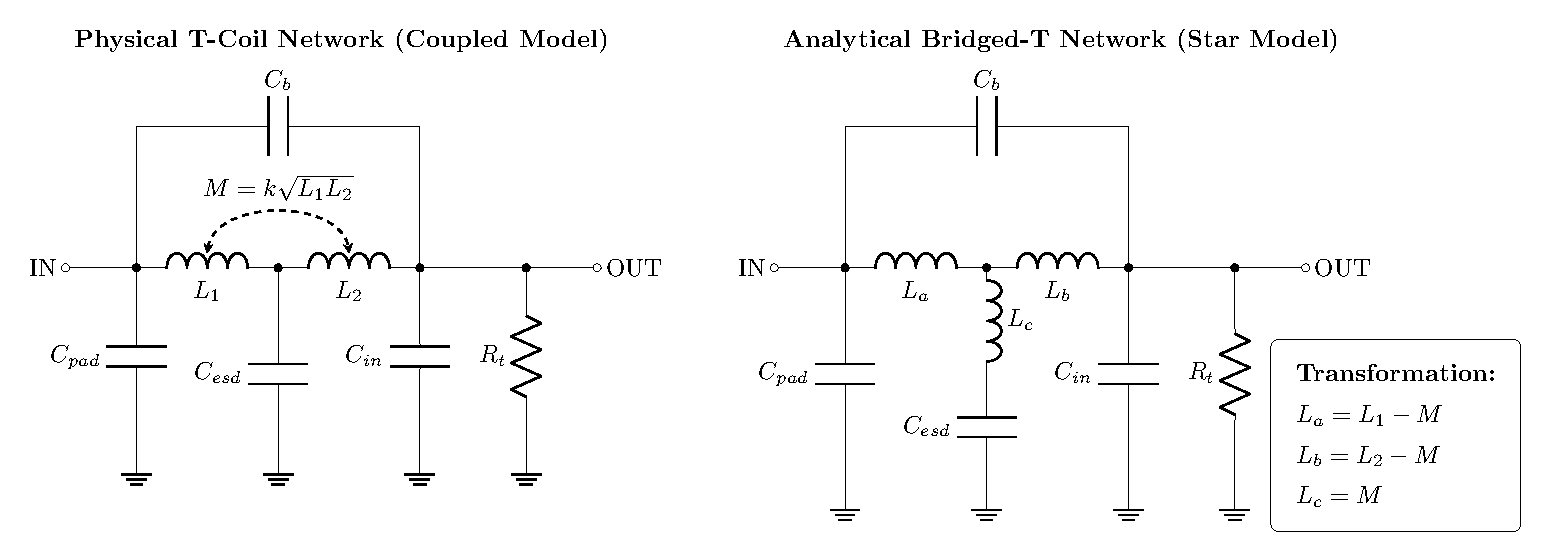
\includegraphics[width=\linewidth]{img/Termination_VGA_img/matlab_model.pdf}
    \caption{Used model for the cascaded ABCD matrix formulation.}
    \label{fig:model_schematic}
\end{figure}

% --- 4-panel MATLAB figure: stacked 1x4 ---
\begin{figure}[H]
    \centering

    % --- First Row ---
    \begin{subfigure}[b]{0.48\textwidth}
        \centering
        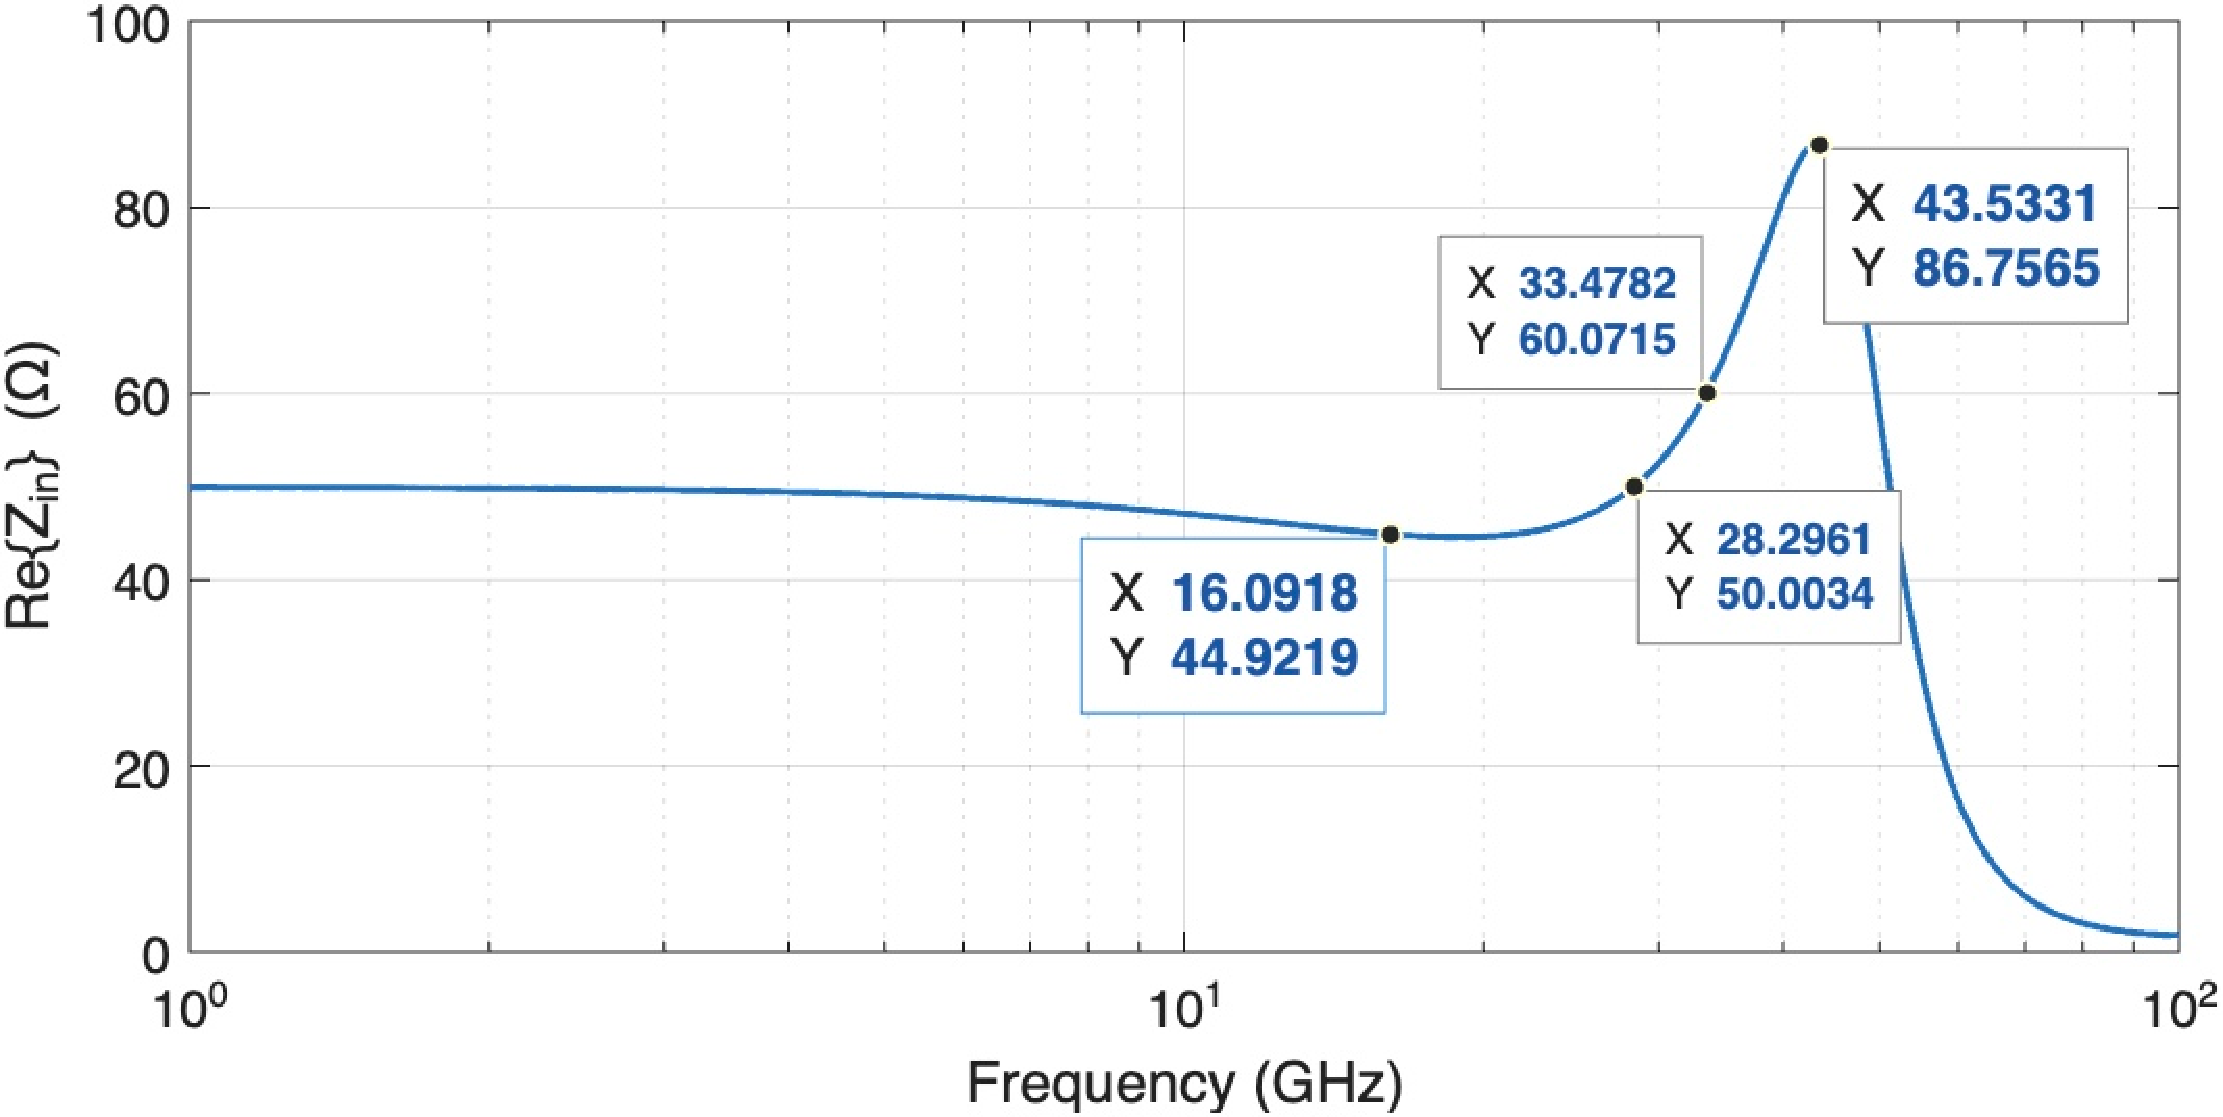
\includegraphics[width=\textwidth]{img/Termination_VGA_img/matlab_re_zin.pdf}
        \caption{Real input impedance, $\text{Re}\{Z_{in}\}$.}
        \label{fig:matlab_re}
    \end{subfigure}
    \hfill
    \begin{subfigure}[b]{0.48\textwidth}
        \centering
        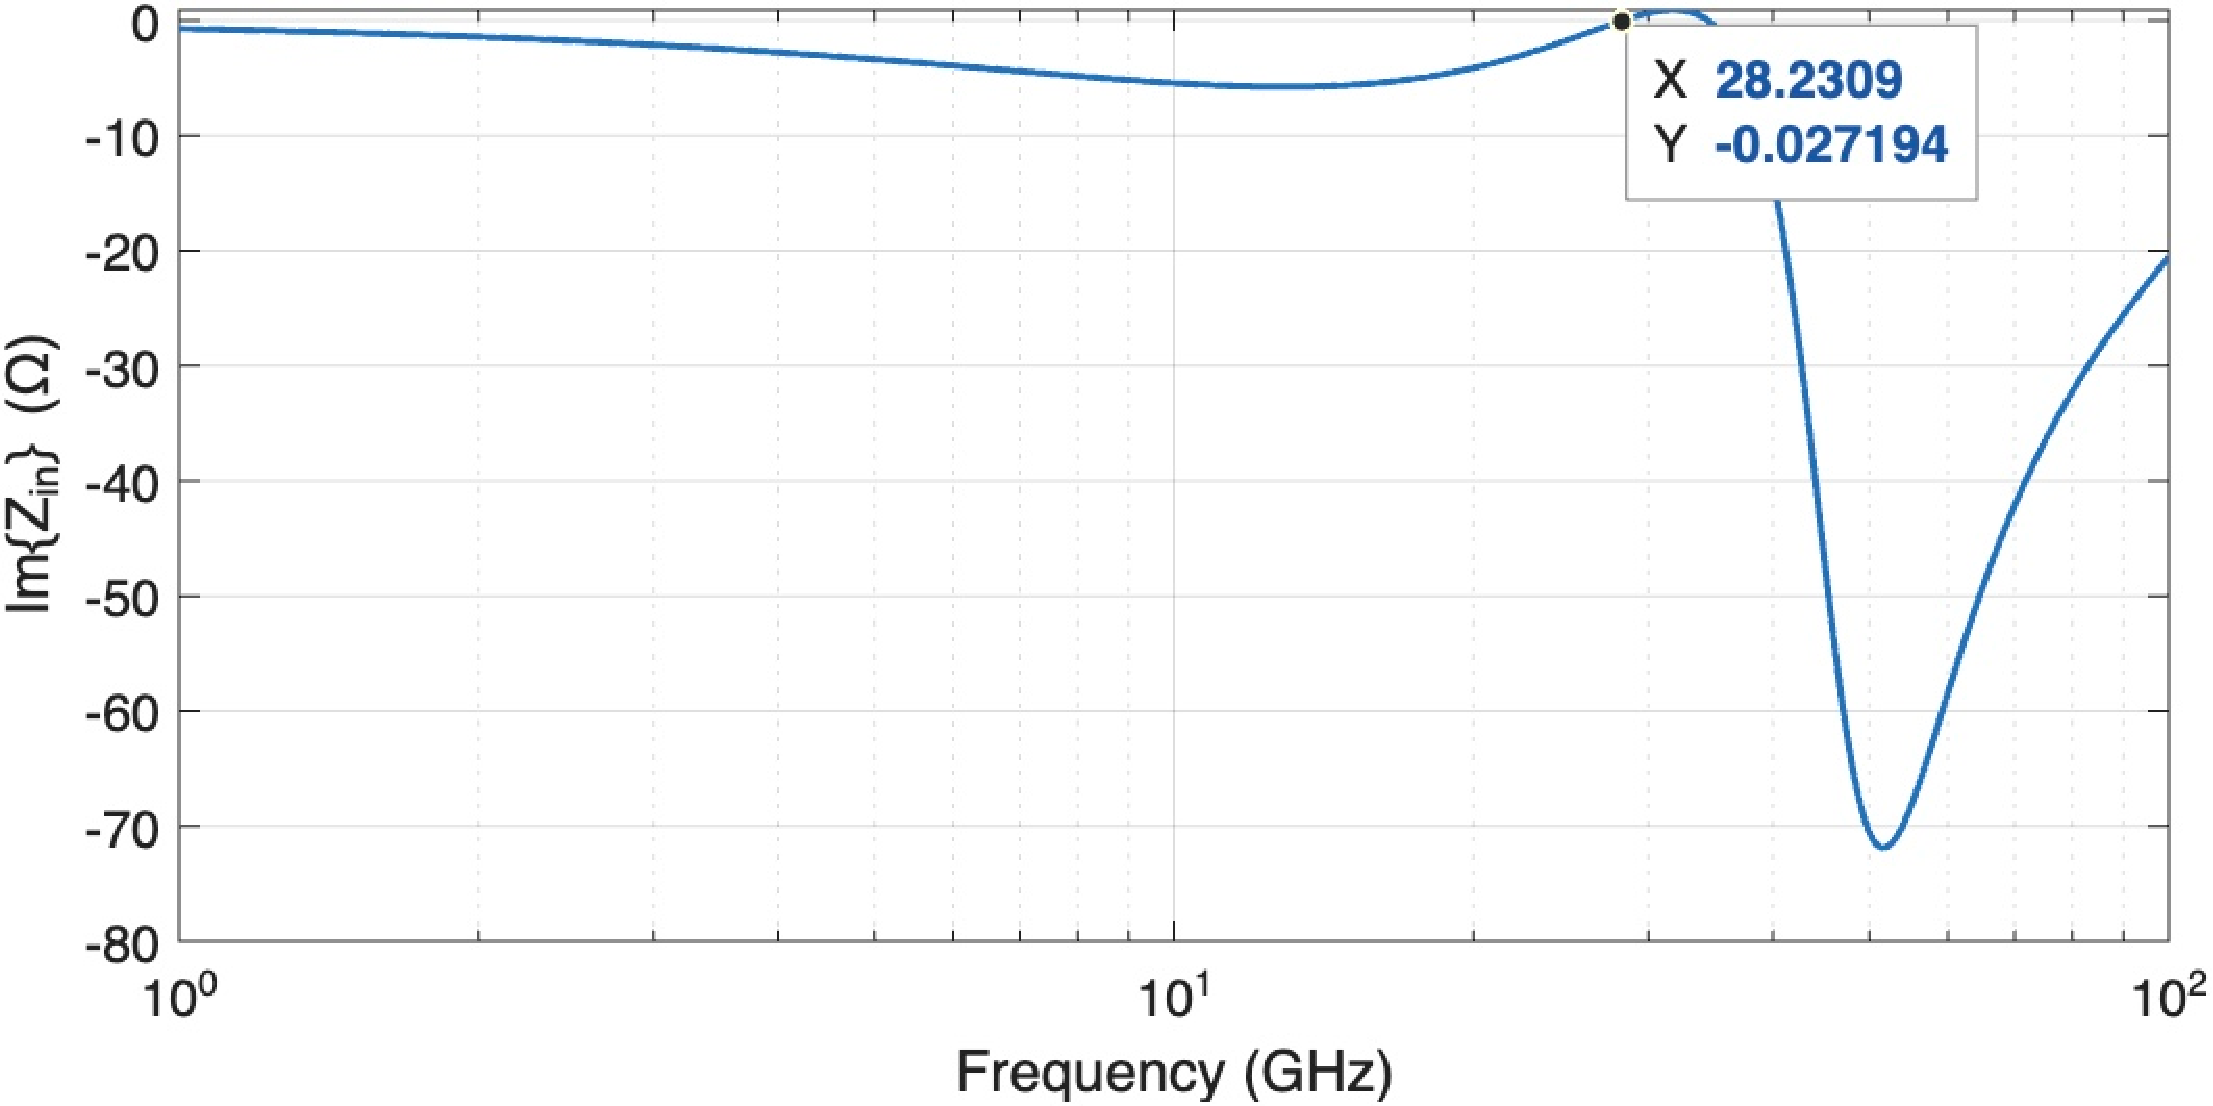
\includegraphics[width=\textwidth]{img/Termination_VGA_img/matlab_im_zin.pdf}
        \caption{Imaginary input impedance, $\text{Im}\{Z_{in}\}$.}
        \label{fig:matlab_im}
    \end{subfigure}

    \vspace{0.4cm} % Space between the top and bottom rows

    % --- Second Row ---
    \begin{subfigure}[b]{0.48\textwidth}
        \centering
        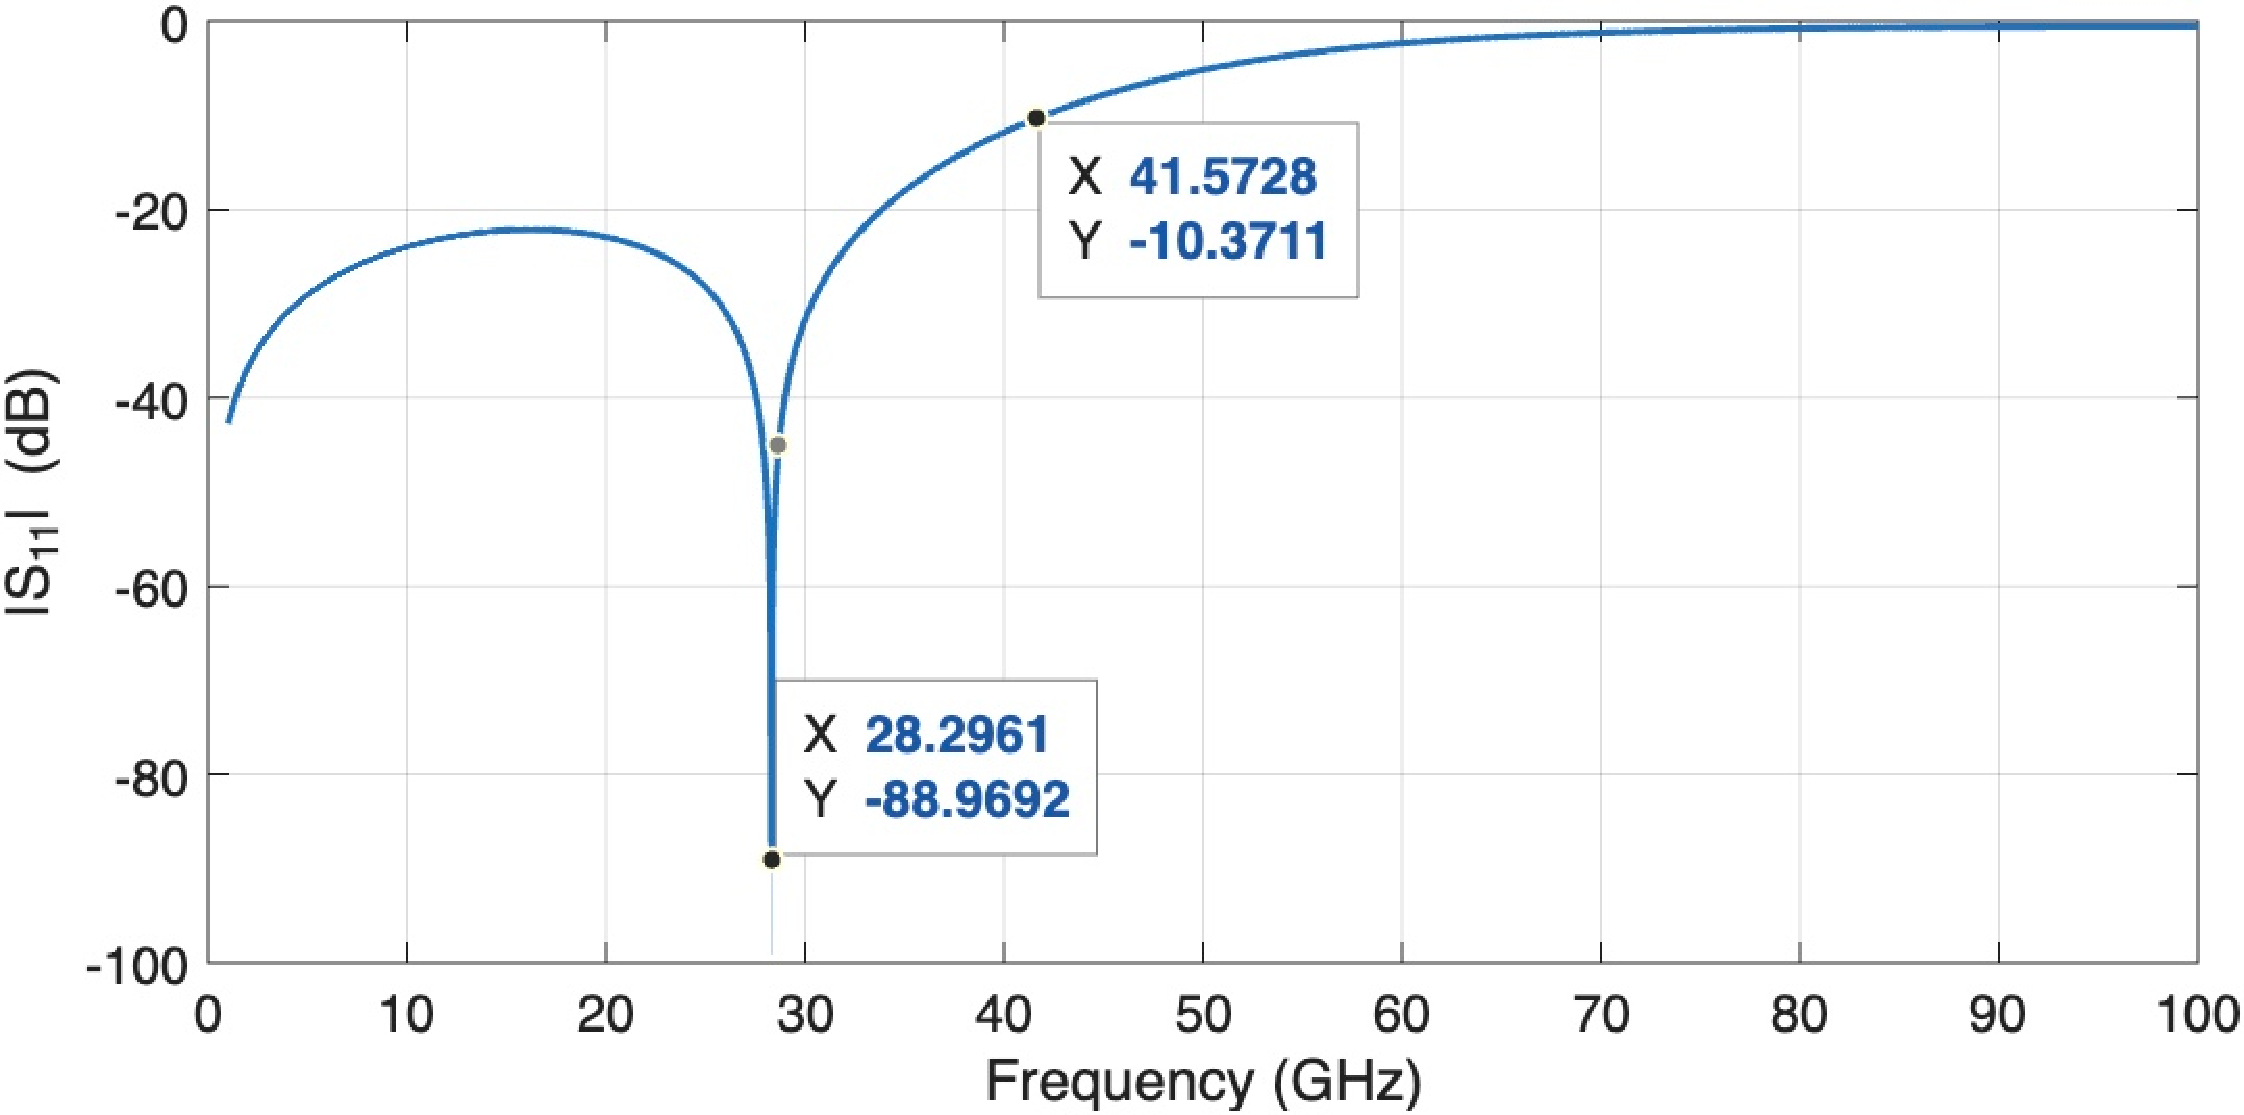
\includegraphics[width=\textwidth]{img/Termination_VGA_img/matlab_s11.pdf}
        \caption{Return loss $S_{11}$ (dB) referenced to $50\,\Omega$.}
        \label{fig:matlab_s11}
    \end{subfigure}
    \hfill
    \begin{subfigure}[b]{0.48\textwidth}
        \centering
        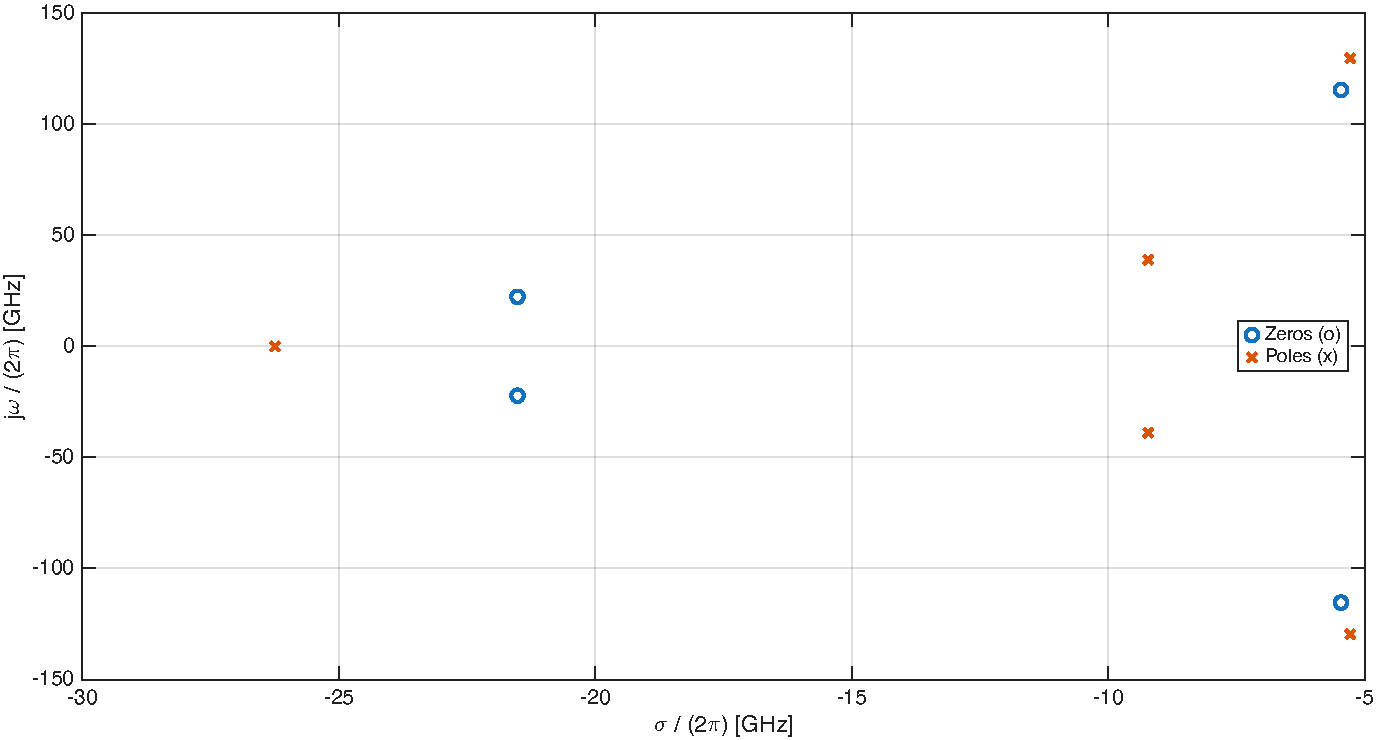
\includegraphics[width=\textwidth]{img/Termination_VGA_img/matlab_pz.pdf}
        \caption{Pole-zero map of $Z_{in}(s)$.}
        \label{fig:matlab_pz}
    \end{subfigure}

    \caption{Analytical MATLAB results for the optimised input network:
             $\text{Re}\{Z_{in}\}$, $\text{Im}\{Z_{in}\}$, $S_{11}$, and the pole-zero map.}
    \label{fig:matlab_analysis}
\end{figure}

% --- Target Values Table ---
\begin{table}[H]
    \centering
    \caption{Target component values}
    \label{tab:target_values}
    \begin{tabular}{@{}lc@{}}
        \toprule
        \textbf{Component Parameter} & \textbf{Target Value} \\
        \midrule
        Self-inductance ($L_1,\,L_2$)  & 130~pH  \\
        Coupling factor ($k$)           & $-0.4$  \\
        Bridging capacitance ($C_b$)    & 9.0~fF  \\
        \bottomrule
    \end{tabular}
\end{table}

% -------------------------------------------------------
\subsection{Proposed Topology}
% -------------------------------------------------------

\subsubsection*{Bridged-T Coil Bandwidth Extension}

A Bridged-T coil topology was selected to achieve the required broadband impedance match.
Unlike a simple series-peaking inductor, the symmetric T-coil exploits mutual coupling
between its two halves to split and absorb the parasitic capacitance of the ESD diode and
the receiver input gate, effectively distributing it across the network. The bridging
capacitor~$C_b$, connected across the outer terminals of the coil, provides an additional
high-frequency feed-forward current path that maintains the real impedance close to $50\,\Omega$
at the upper edge of the passband, where the inductors would otherwise present a high impedance.

\newpage
\subsubsection*{Digitally Controlled Impedance (DCI)}

Polysilicon resistors are subject to process and temperature (PT) variation of up to
$\pm 20\%$, which would cause a static resistor termination to drift well outside the
required $50\,\Omega$ window. To guarantee compliance across all corners, an active
Digitally Controlled Impedance (DCI) network was designed.

\vspace{\baselineskip}

The DCI employs a complementary topology: a PMOS pull-up network~($R_{UP}$) and an NMOS
pull-down network~($R_{Down}$) are connected in parallel between supply and ground at
the input node. This structure serves a dual purpose. First, the parallel combination of
the two branches sets the AC termination impedance seen by the channel:
\begin{equation}
    R_{Term} = \frac{R_{UP} \cdot R_{Down}}{R_{UP} + R_{Down}} = 50\,\Omega
    \label{eq:rterm}
\end{equation}
Second, the same resistive divider establishes the DC common-mode voltage at the input node:
\begin{equation}
    V_{CM} = V_{DD} \cdot \frac{R_{Down}}{R_{UP} + R_{Down}}
    \label{eq:vcm}
\end{equation}
Solving Equations~\eqref{eq:rterm} and~\eqref{eq:vcm} simultaneously for the target
$V_{CM} = 540\,\text{mV}$ and $V_{DD} = 0.9\,\text{V}$ yields $R_{UP} = 74.1\,\Omega$
and $R_{Down} = 153.8\,\Omega$.

\vspace{\baselineskip}

To counter PT variation, each branch implements a 4-bit binary-weighted tuning array.
An always-on base leg is sized to achieve the target resistance at the fastest (FF) process
corner, where resistors are at their minimum value. For slower corners, the four binary
tuning legs add parallel conductance in discrete steps. The target resistance of each
tuning branch follows a binary scaling law:
\begin{equation}
    R_{branch,\,n} = \frac{R_{branch,\,0}}{2^{n}}, \quad n = 0, 1, 2, 3
    \label{eq:rbranch}
\end{equation}
Because each tuning switch contributes a finite ON-resistance ($R_{SW}$), the physical
polysilicon resistor drawn in layout is reduced by that amount to preserve the target
branch resistance:
\begin{equation}
    R_{Drawn} = R_{branch,\,n} - R_{SW}
    \label{eq:rdrawn}
\end{equation}

The schematic of the proposed input network topology is shown in
Figure~\ref{fig:input_schematic}, and the full DCI circuit implementation is shown in
Figure~\ref{fig:dci_schematic}.

\begin{figure}[H]
    \centering
    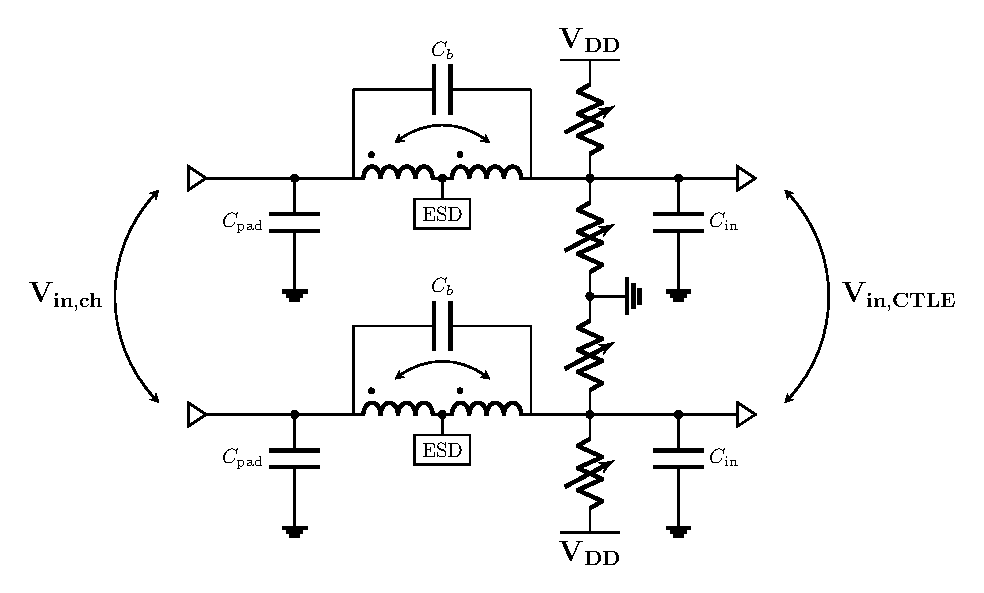
\includegraphics[width=0.75\textwidth]{img/Termination_VGA_img/input_network_sch.pdf}
    \caption{Proposed Bridged-T input network schematic, showing the differential
             T-coil pair, ESD protection, $C_b$, $C_{in}$, and the DCI termination.}
    \label{fig:input_schematic}
\end{figure}

\begin{figure}[H]
    \centering
    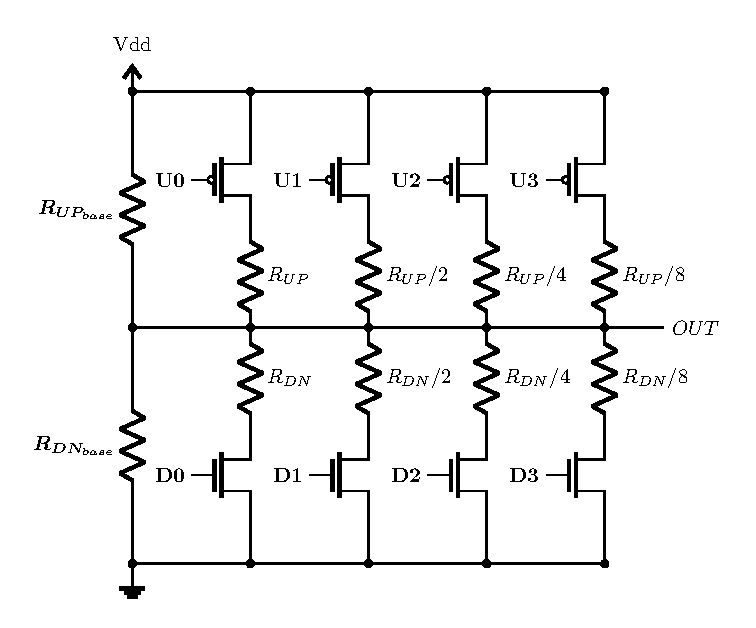
\includegraphics[width=0.7\textwidth]{img/Termination_VGA_img/DCI_sch.pdf}
    \caption{Complementary PMOS/NMOS Digitally Controlled Impedance (DCI)
             circuit, showing the always-on base leg and the four binary tuning branches.}
    \label{fig:dci_schematic}
\end{figure}

% -------------------------------------------------------
\subsection{Implementation and Simulation Results}
% -------------------------------------------------------

\subsubsection{T-Coil Design and EMX Extraction}

The T-coil was implemented as an octagonal symmetric spiral on the thick top metal layers to
maximise the quality factor~$Q$. The geometry was iteratively optimised in EMX to simultaneously
meet the self-inductance and coupling factor targets derived from the analytical model.
The extracted frequency-dependent parameters are plotted in Figure~\ref{fig:tcoil_emx_full},
and the physical layout dimensions together with the achieved parasitic values are
summarised in Tables~\ref{tab:tcoil_dims} and~\ref{tab:achieved_values} respectively.

% --- T-coil EMX results: 2x2 grid ---
\begin{figure}[H]
    \centering
    \begin{subfigure}[b]{0.48\textwidth}
        \centering
        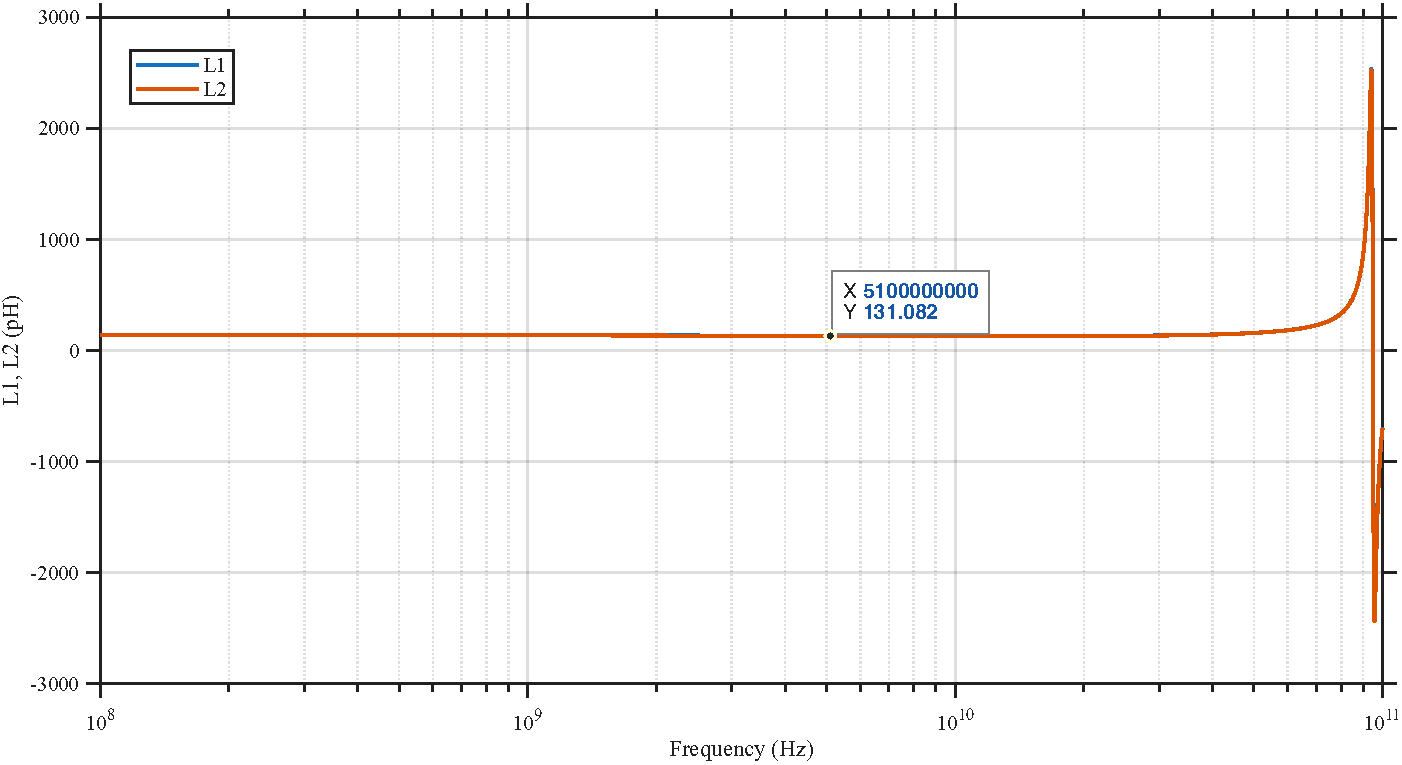
\includegraphics[width=\textwidth]{img/Termination_VGA_img/tcoil_L.pdf}
        \caption{Self-inductance $L_1,\,L_2$ vs.\ frequency.}
        \label{fig:tcoil_L}
    \end{subfigure}
    \hfill
    \begin{subfigure}[b]{0.48\textwidth}
        \centering
        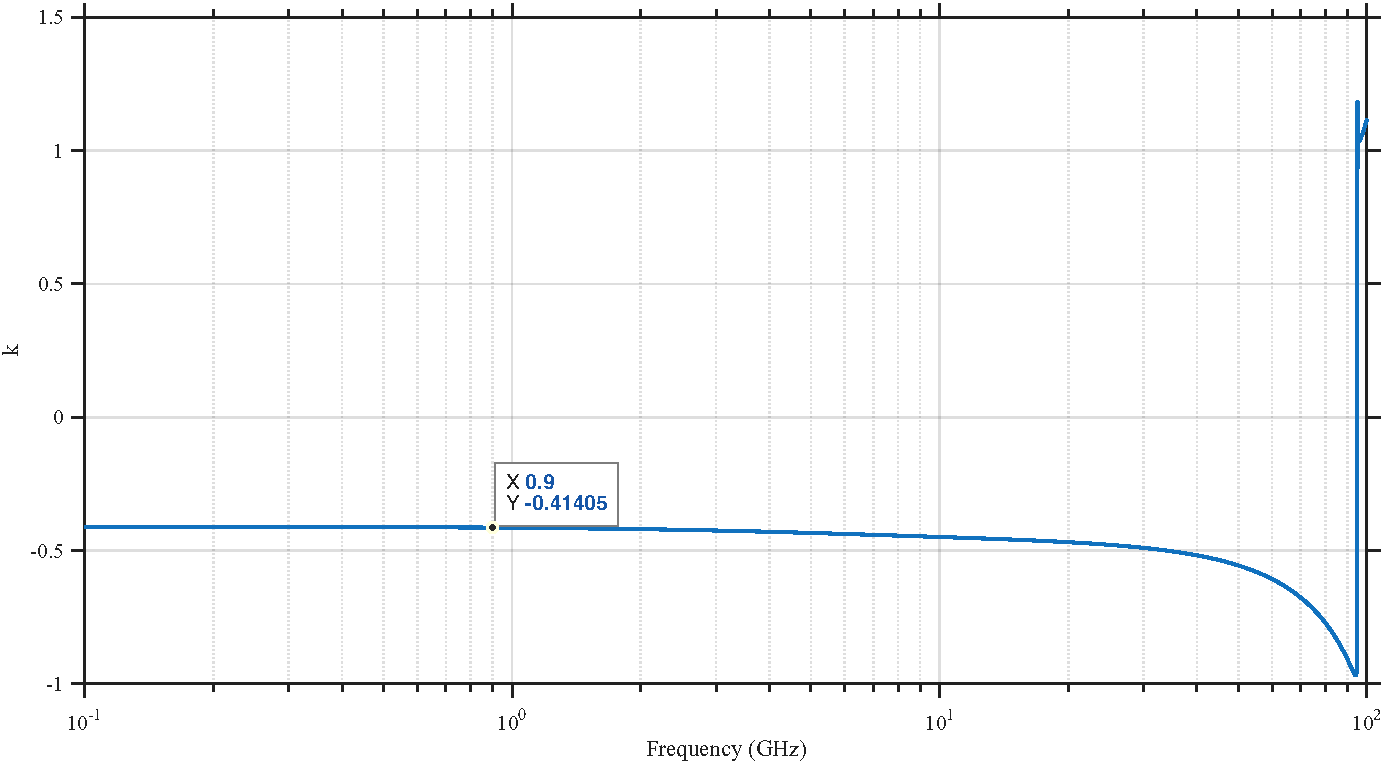
\includegraphics[width=\textwidth]{img/Termination_VGA_img/tcoil_k.pdf}
        \caption{Coupling factor $k$ vs.\ frequency.}
        \label{fig:tcoil_k}
    \end{subfigure}

    \vspace{10pt}

    \begin{subfigure}[b]{0.48\textwidth}
        \centering
        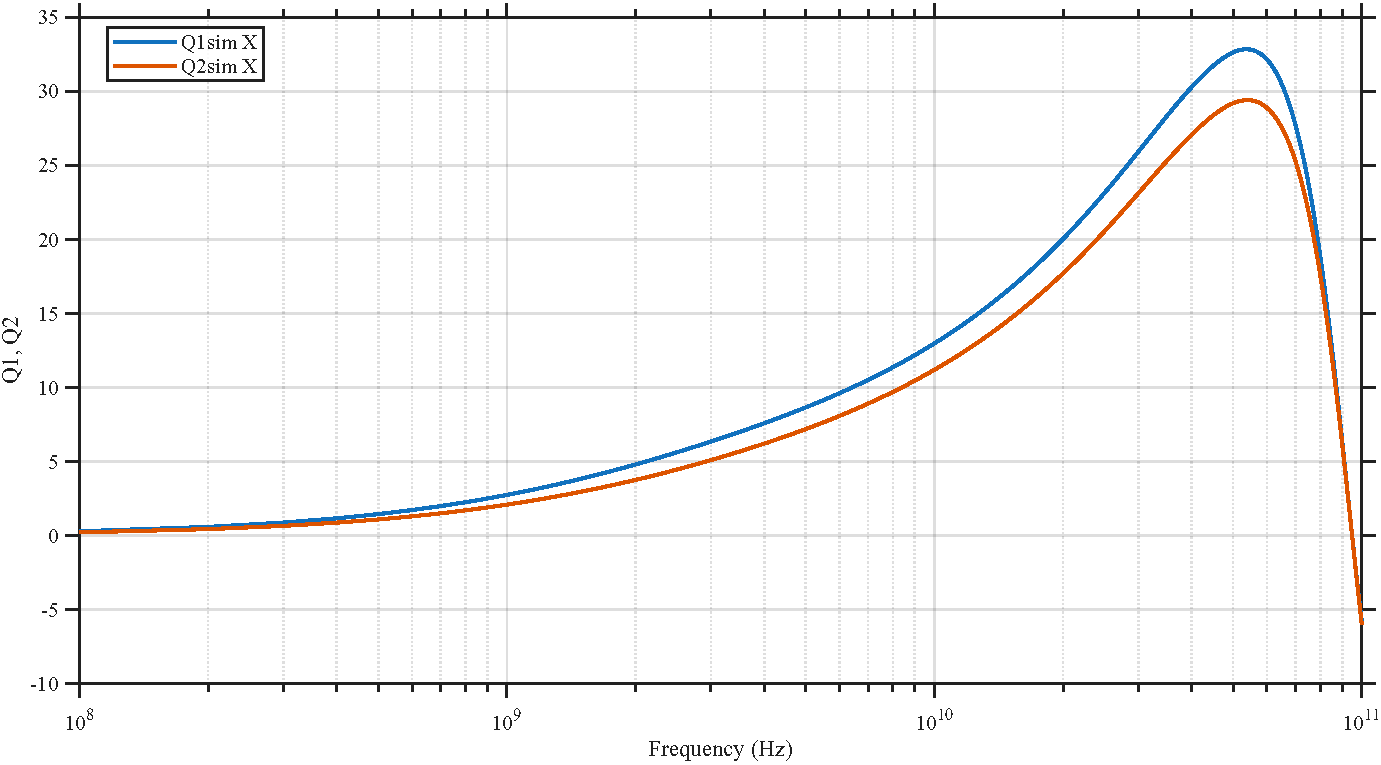
\includegraphics[width=\textwidth]{img/Termination_VGA_img/tcoil_Q.pdf}
        \caption{Quality factor $Q$ vs.\ frequency.}
        \label{fig:tcoil_Q}
    \end{subfigure}
    \hfill
    \begin{subfigure}[b]{0.48\textwidth}
        \centering
        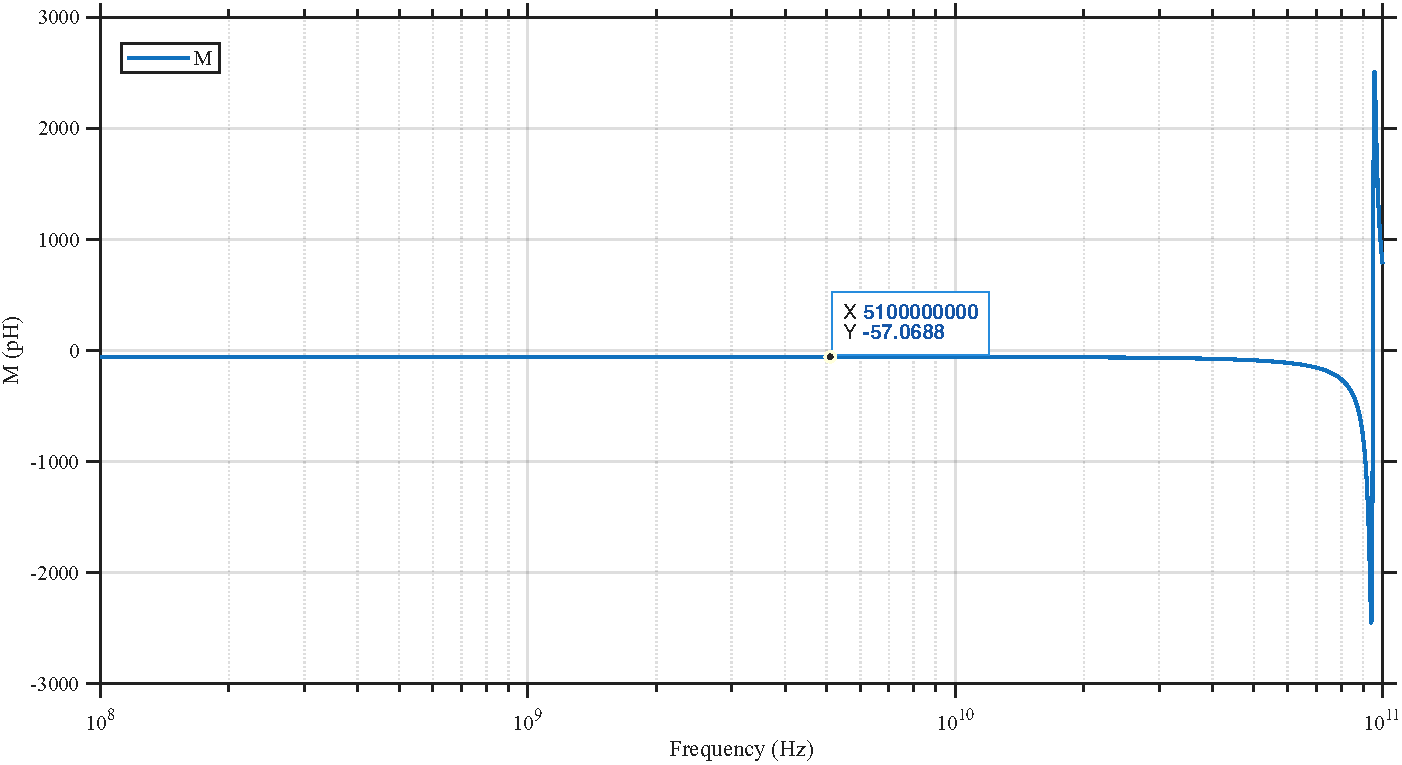
\includegraphics[width=\textwidth]{img/Termination_VGA_img/tcoil_M.pdf}
        \caption{Mutual inductance $M$ vs.\ frequency.}
        \label{fig:tcoil_M}
    \end{subfigure}

    \caption{EMX post-layout simulation results for the T-coil: self-inductance,
             coupling factor, quality factor, and mutual inductance across frequency.}
    \label{fig:tcoil_emx_full}
\end{figure}

\begin{figure}[H]
    \centering
    % --- Left side: The Layout Figure ---
    \begin{minipage}[c]{0.45\textwidth}
        \centering
        % \textwidth here refers to the width of the minipage
        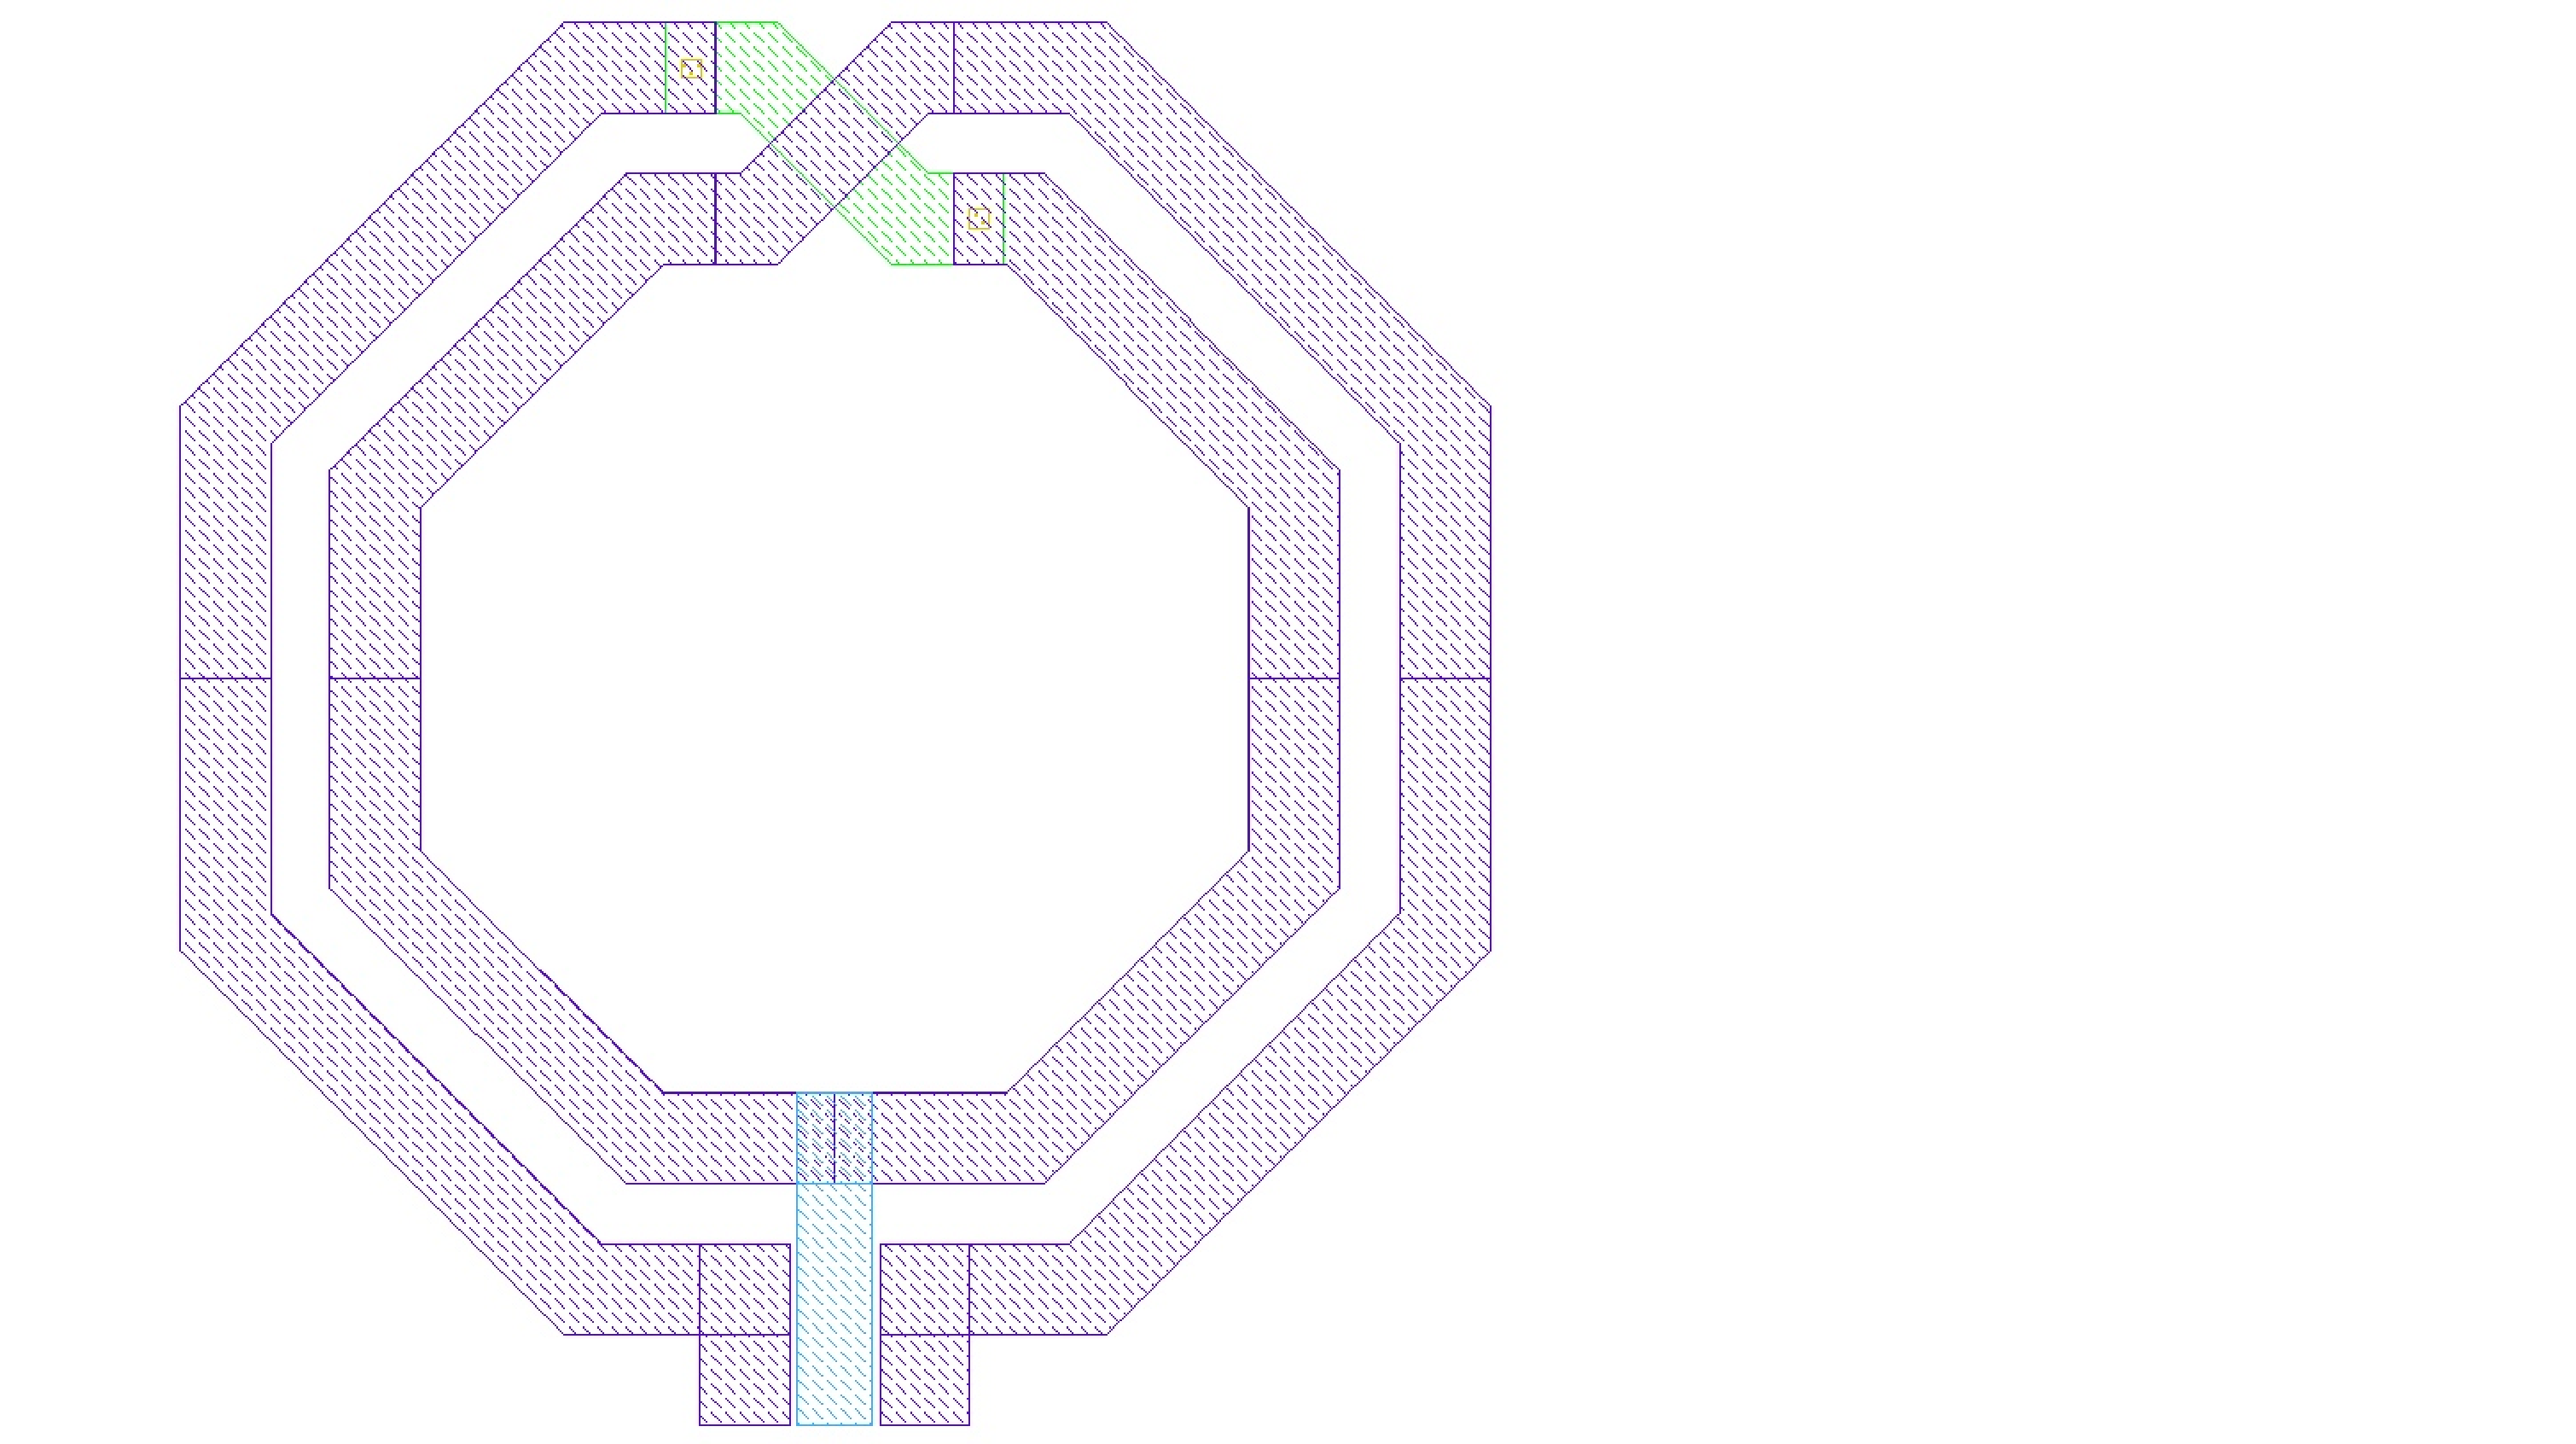
\includegraphics[width=0.7\textwidth]{img/Termination_VGA_img/tcoil_layout.pdf}
        \caption{Octagonal T-coil layout.}
        \label{fig:tcoil_layout}
    \end{minipage}\hfill
    % --- Right side: The Dimensions Table ---
    \begin{minipage}[c]{0.45\textwidth}
        \centering
        \captionof{table}{T-Coil Physical Dimensions}
        \label{tab:tcoil_dims}
        \begin{tabular}{@{}ll@{}}
            \toprule
            \textbf{Parameter}          & \textbf{Value}     \\
            \midrule
            Outer diameter ($OD$)       & $87\,\mu\text{m}$  \\
            Inner diameter ($ID$)       & $55\,\mu\text{m}$  \\
            Trace width ($W$)           & $6\,\mu\text{m}$   \\
            Turn spacing ($S$)          & $4\,\mu\text{m}$   \\
            Number of turns ($N$)       & 2                  \\
            \bottomrule
        \end{tabular}
    \end{minipage}
\end{figure}

\begin{table}[H]
    \centering
    \caption{T-coil parameters extracted from EMX}
    \label{tab:achieved_values}
    \begin{tabular}{@{}lcc@{}}
        \toprule
        \textbf{Parameter}              & \textbf{Target} & \textbf{Achieved (EMX)} \\
        \midrule
        Self-inductance ($L_1,\,L_2$)   & 130~pH          & 131~pH                  \\
        Coupling factor ($k$)           & $-0.4$          & $-0.41$                 \\
        \bottomrule
    \end{tabular}
\end{table}

\subsubsection{DCI Performance Across Corners}

The robustness of the DCI performance was evaluated across extreme process and temperature corners. As summarized in Table~\ref{tab:vcm_corners}, the output common-mode voltage ($V_{CM}$) exhibits exceptional stability. Thanks to the calibration framework, the total $V_{CM}$ deviation is tightly constrained to within $\pm 1\,\text{mV}$ of the nominal target across all simulated conditions. Furthermore, the 4-bit tuning array successfully regulates the input impedance, maintaining the nominal $50\,\Omega$ termination with a maximum worst-case variation of less than $4\,\Omega$.

\begin{table}[H]
    \centering
    \caption{Common-mode voltage ($V_{CM}$) and termination stability across PVT corners}
    \label{tab:vcm_corners}
    \begin{tabular}{@{}lccccc@{}}
        \toprule
        \textbf{Parameter} & \textbf{Nominal} & \textbf{SS, $125^\circ$C} & \textbf{SS, $-40^\circ$C} & \textbf{FF, $125^\circ$C} & \textbf{FF, $-40^\circ$C} \\
        \midrule
        $V_{CM}$ (mV) & 540.9 & 541.5 & 540.7 & 540.3 & 541.4 \\
        $R_{Term}$ ($\Omega$) & 49.87 & 53.56 & 52.11 & 50.58 & 49.86 \\
        \bottomrule
    \end{tabular}
\end{table}

% -------------------------------------------------------
\subsubsection{Complete Input Network Testbench}
% -------------------------------------------------------
 
The full top-level simulation was conducted using the differential testbench illustrated in Figure~\ref{fig:full_tb}. The architecture consists of two identical single-ended input network instances configured differentially. Each half-circuit integrates the fully extracted post-layout T-coil, the DCI termination network, and lumped models representing the front-end parasitic capacitances ($C_{pad} = 50\,\text{fF}$, $C_{ESD} = 60\,\text{fF}$, and $C_{in} = 35\,\text{fF}$).

In accordance with PCI-SIG specifications, a $265\,\text{nF}$ AC coupling capacitor ($C_c$) is placed in series with the input port. Its impedance is negligible at high frequencies ($|Z_{C_c}| < 1\,\text{m}\Omega$ at $1\,\text{GHz}$), ensuring it does not affect the AC response. Its primary purpose is to provide required DC isolation by blocking the $540\,\text{mV}$ DCI common-mode bias from reaching the $50\,\Omega$ measurement port.

The DCI digital interface is driven by a custom Verilog-A behavioral decoder (\texttt{DCIctrl}). This block translates a single parametric DC voltage into the 4-bit binary control code (UP$\langle$3:0$\rangle$ and DN$\langle$3:0$\rangle$) required to tune the termination matrix.

\begin{figure}[H]
    \centering
    \framebox{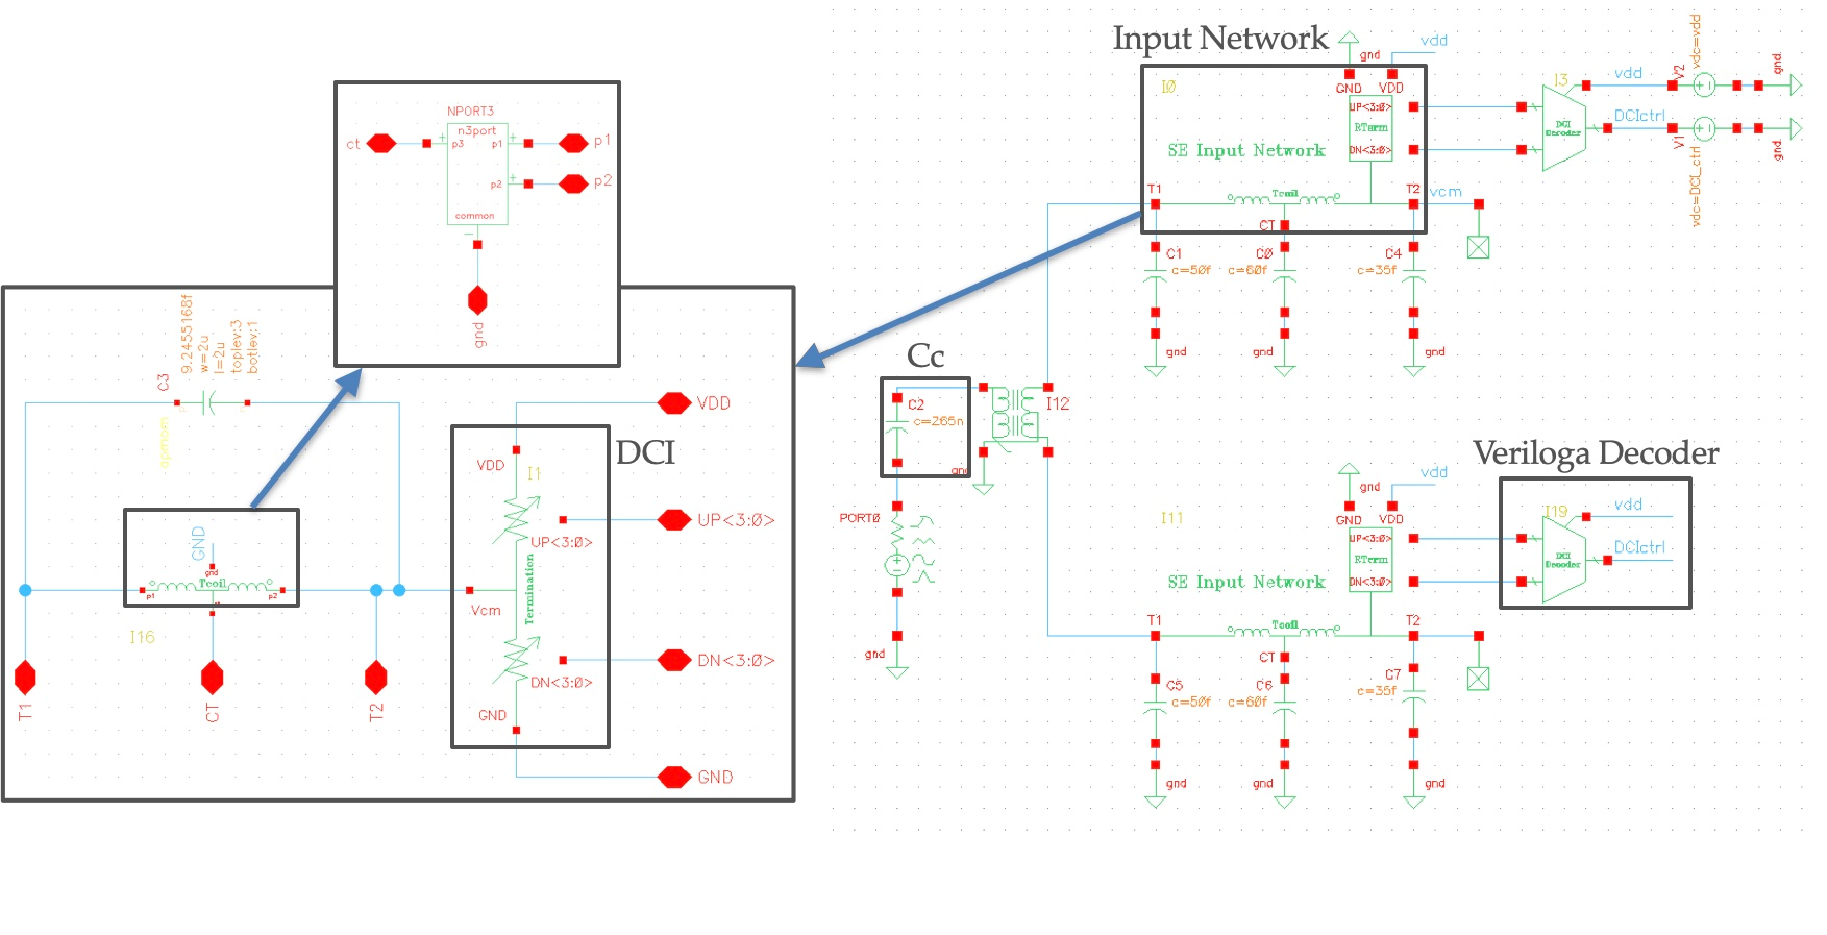
\includegraphics[width=0.95\textwidth]{img/Termination_VGA_img/testbenchinput.pdf}}
    \caption{Differential input network simulation testbench.}
    \label{fig:full_tb}
\end{figure}

\subsubsection{Overall Input Network Performance}
As illustrated in Figure~\ref{fig:overall_perf}, the input network exhibits broadband matching performance that significantly exceeds the PCI-SIG compliance mask. The standard dictates a differential return loss ($S_{11}$) strictly below $-10\,\text{dB}$ up to $1.25\,\text{GHz}$, relaxing to $-8\,\text{dB}$ up to $16\,\text{GHz}$. In contrast, the proposed design effortlessly maintains an $S_{11}$ below $-10\,\text{dB}$ across an extended bandwidth up to $35\,\text{GHz}$. Furthermore, the real input impedance ($R_{in}$) remains tightly bounded between $40\,\Omega$ and $60\,\Omega$ up to $25\,\text{GHz}$, ensuring robust signal integrity.

% --- Overall performance: stacked 2x1 ---
\begin{figure}[H]
    \centering

    \begin{subfigure}[b]{0.9\textwidth}
        \centering
        \framebox{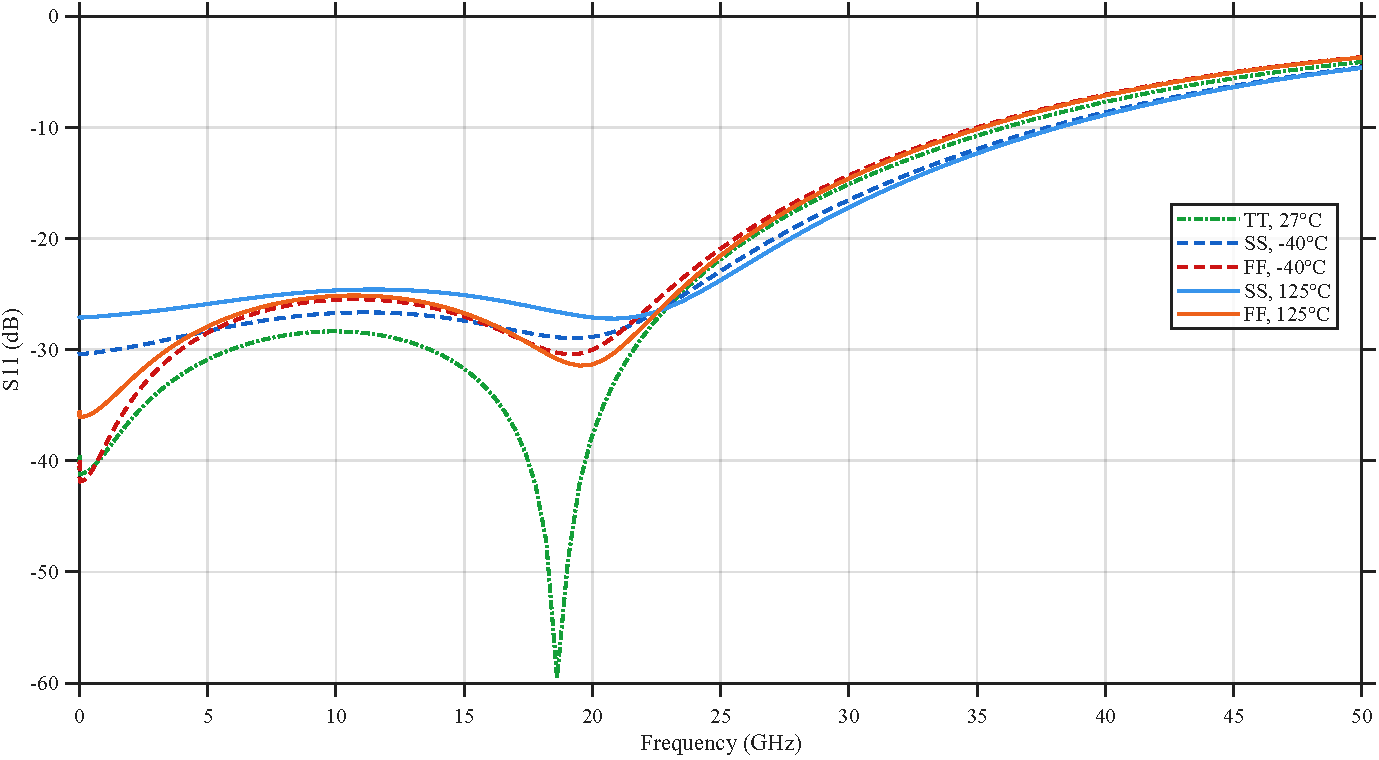
\includegraphics[width=\textwidth]{img/Termination_VGA_img/in_S11.pdf}}
        \caption{Overall Input Network $S_{11}$}
        \label{fig:overall_s11}
    \end{subfigure}

    \vspace{1cm}

    \begin{subfigure}[b]{0.9\textwidth}
        \centering
        \framebox{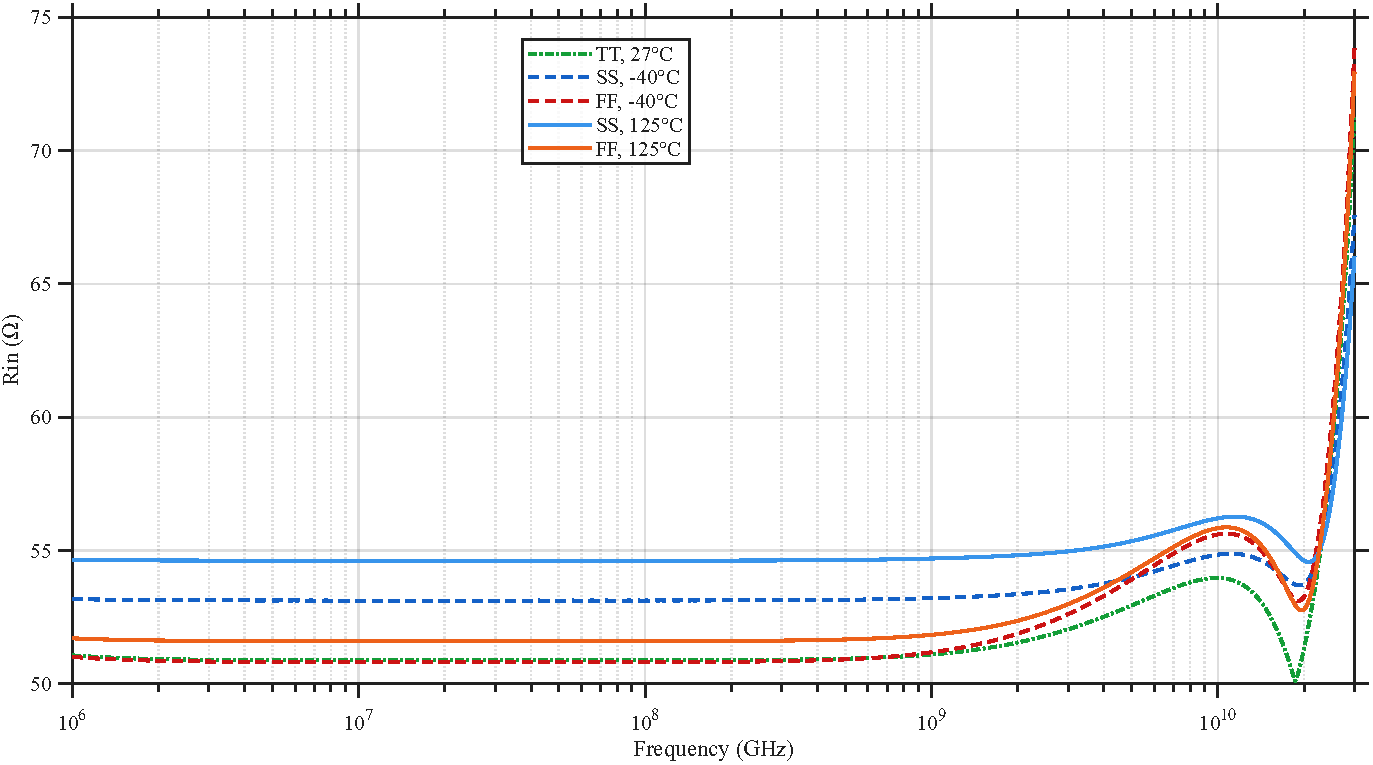
\includegraphics[width=.95\textwidth]{img/Termination_VGA_img/in_Rin.pdf}}
        \caption{Overall Real Input Impedance $R_{in}$}
        \label{fig:overall_rin}
    \end{subfigure}

    \caption{Top-level AC performance of the complete receiver input network.}
    \label{fig:overall_perf}
\end{figure}
 

\newpage
\section{Variable Gain Amplifier (VGA)}

\newpage
\section{Continous Time Linear Equalizer (CTLE)}
\section*{PCIe 6.0 CTLE Specifications}
\label{ch:specs}

\section*{PCIe 6.0 Equalization Requirements}
The evolution of peripheral component interconnects to the PCIe 6.0 standard introduces a target data rate of 64.0 GT/s. At these extremely high transmission speeds, signals traveling over copper traces experience severe, frequency-dependent insertion loss. This attenuation disproportionately degrades the high-frequency components of the transmitted signal, leading to severe Inter-Symbol Interference (ISI) at the receiver. To reliably recover the data and maintain the required Bit Error Rate (BER), robust equalization is critical. Consequently, the PCIe 6.0 specification mandates the use of a high-order behavioral Continuous-Time Linear Equalizer (CTLE) within the reference receiver model. 

The primary function of this CTLE is to provide high-frequency peaking that operates inversely to the channel's insertion loss profile. By carefully tuning the CTLE transfer function, the overall system response (Channel + CTLE) is flattened across the Nyquist bandwidth, significantly opening the received data eye prior to further digital equalization stages such as Decision Feedback Equalization (DFE).

\newpage
\section*{Behavioral CTLE Specifications}
To achieve the shaping flexibility necessary to compensate for a wide variety of standard channel models, the behavioral CTLE defined for the 64.0 GT/s data rate consists of a complex transfer function featuring six poles and three zeros. This is typically modeled as a series of cascaded stages to achieve the required high-order shaping, as illustrated in Figure~\ref{fig:behav_model_stages}.

\begin{figure}[H]
    \centering
    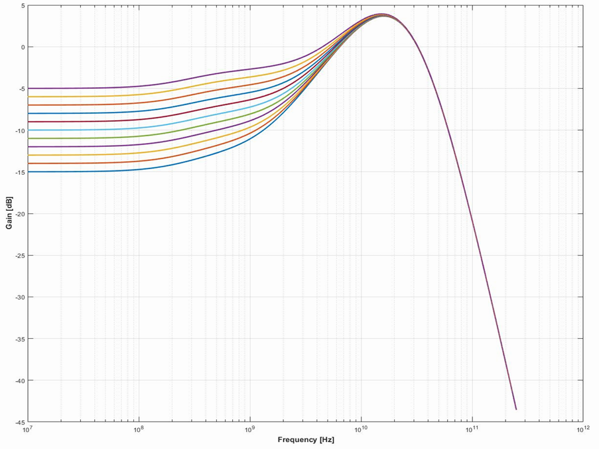
\includegraphics[width=\textwidth]{img/CTLE_img/pcie6_standard_extracted_behav_model_ctle.png}
    \caption{Cascaded CTLE stages extracted from the PCIe 6.0 standard behavioral model.}
    \label{fig:behav_model_stages}
\end{figure}

\noindent A critical component of this behavioral model is its highly adjustable DC gain parameter. The standard specifies strict boundaries and granularities for this tuning to ensure reliable compensation across different physical routing environments. 

\newpage \noindent The target specifications extracted from the PCIe 6.0 standard, which serve as foundational design constraints throughout this work, are provided in Figure~\ref{fig:ctle_spec_img} and summarized in Table~\ref{tab:specs}.

\begin{figure}[H]
    \centering
    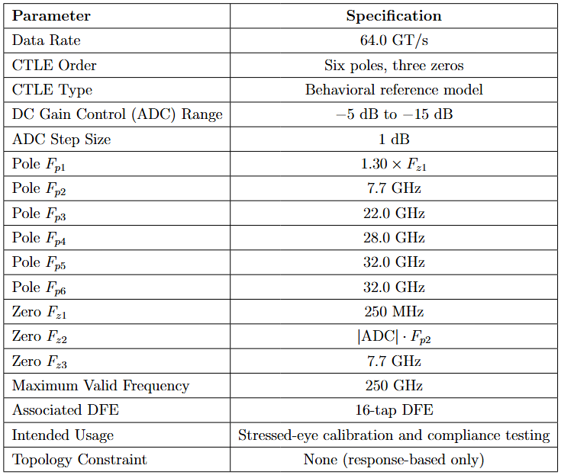
\includegraphics[width=0.8\textwidth]{img/CTLE_img//pcie6_standard_ctle_spec.png}
    \caption{Target CTLE specifications extracted from the PCIe 6.0 standard.}
    \label{fig:ctle_spec_img}
\end{figure}

\begin{table}[H]
    \centering
    \caption{Summary of the CTLE design specs extracted from the PCIe 6.0 standard.}
    \label{tab:specs}
    \renewcommand{\arraystretch}{1.2}
    \begin{tabular}{@{}lcc@{}}
        \toprule
        \textbf{Parameter}    & \textbf{Specification}       & \textbf{Unit} \\
        \midrule
        Supply voltage        & $0.8 \pm 5\%$    & V             \\
        Data rate             & 64               & Gb/s          \\
        DC gain range         & $-5$ to $-15$    & dB            \\
        DC gain step size     & 1                & dB            \\
        Maximum HF boost      & 19               & dB            \\
        Current consumption     & $< 20$           & mA            \\
        Temperature range     & $-40$ to $+120$  & \si{\celsius} \\
        \bottomrule
    \end{tabular}
\end{table}

\noindent The maximum high-frequency boost of 19 dB is essential for deep-insertion-loss channels, while the 1 dB step size allows the receiver adaptation algorithms to finely tune the equalization profile without over-amplifying high-frequency noise or crosstalk.

\section*{Channel Model Characteristics and Test Setup}
Validating the behavioral model requires a robust transient and AC simulation environment. The channel model dictates the baseline amount of equalization required. For this testbench, the physical channel was constructed by cascading a fundamental 1-inch FR4 segment, illustrated in Figure~\ref{fig:channel_model}. 

\begin{figure}[H]
    \centering
    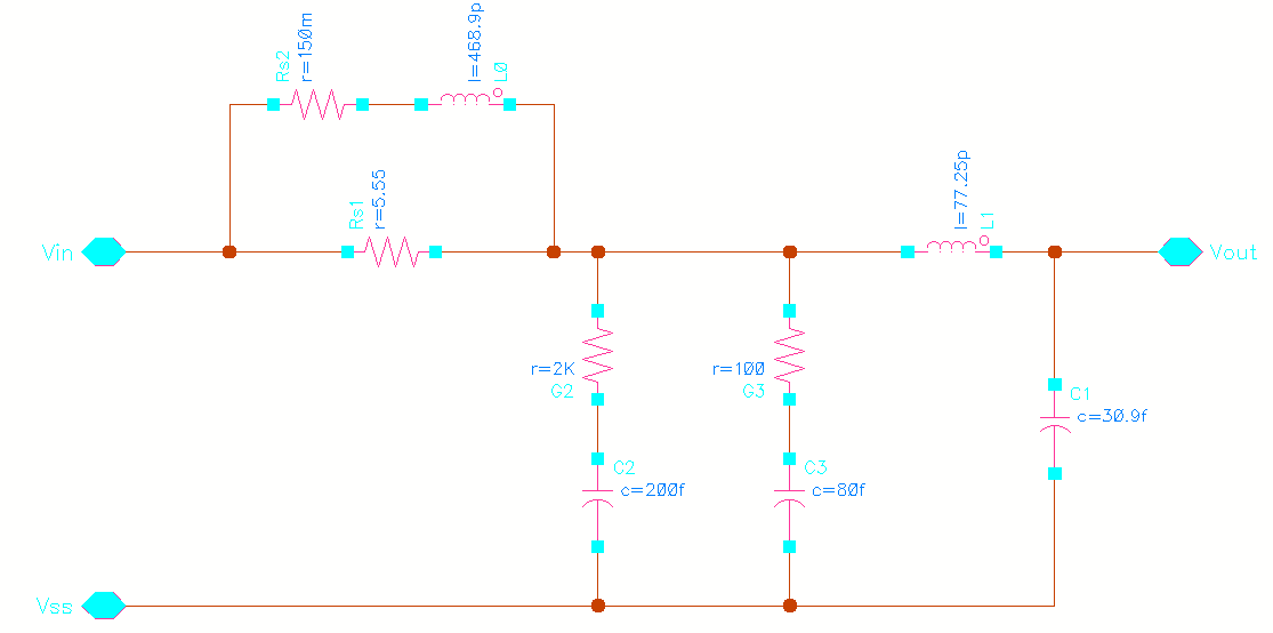
\includegraphics[width=0.8\textwidth]{img/CTLE_img/channel_model.png}
    \caption{The 1-inch FR4 segment used as the fundamental building block to construct the physical channel model.}
    \label{fig:channel_model}
\end{figure}

\noindent This cascaded configuration results in a severe channel model exhibiting an insertion loss of approximately $-$26 dB at the Nyquist frequency. This deep-loss profile is utilized to strictly evaluate the CTLE's compensation limits.

\begin{figure}[H]
    \centering
    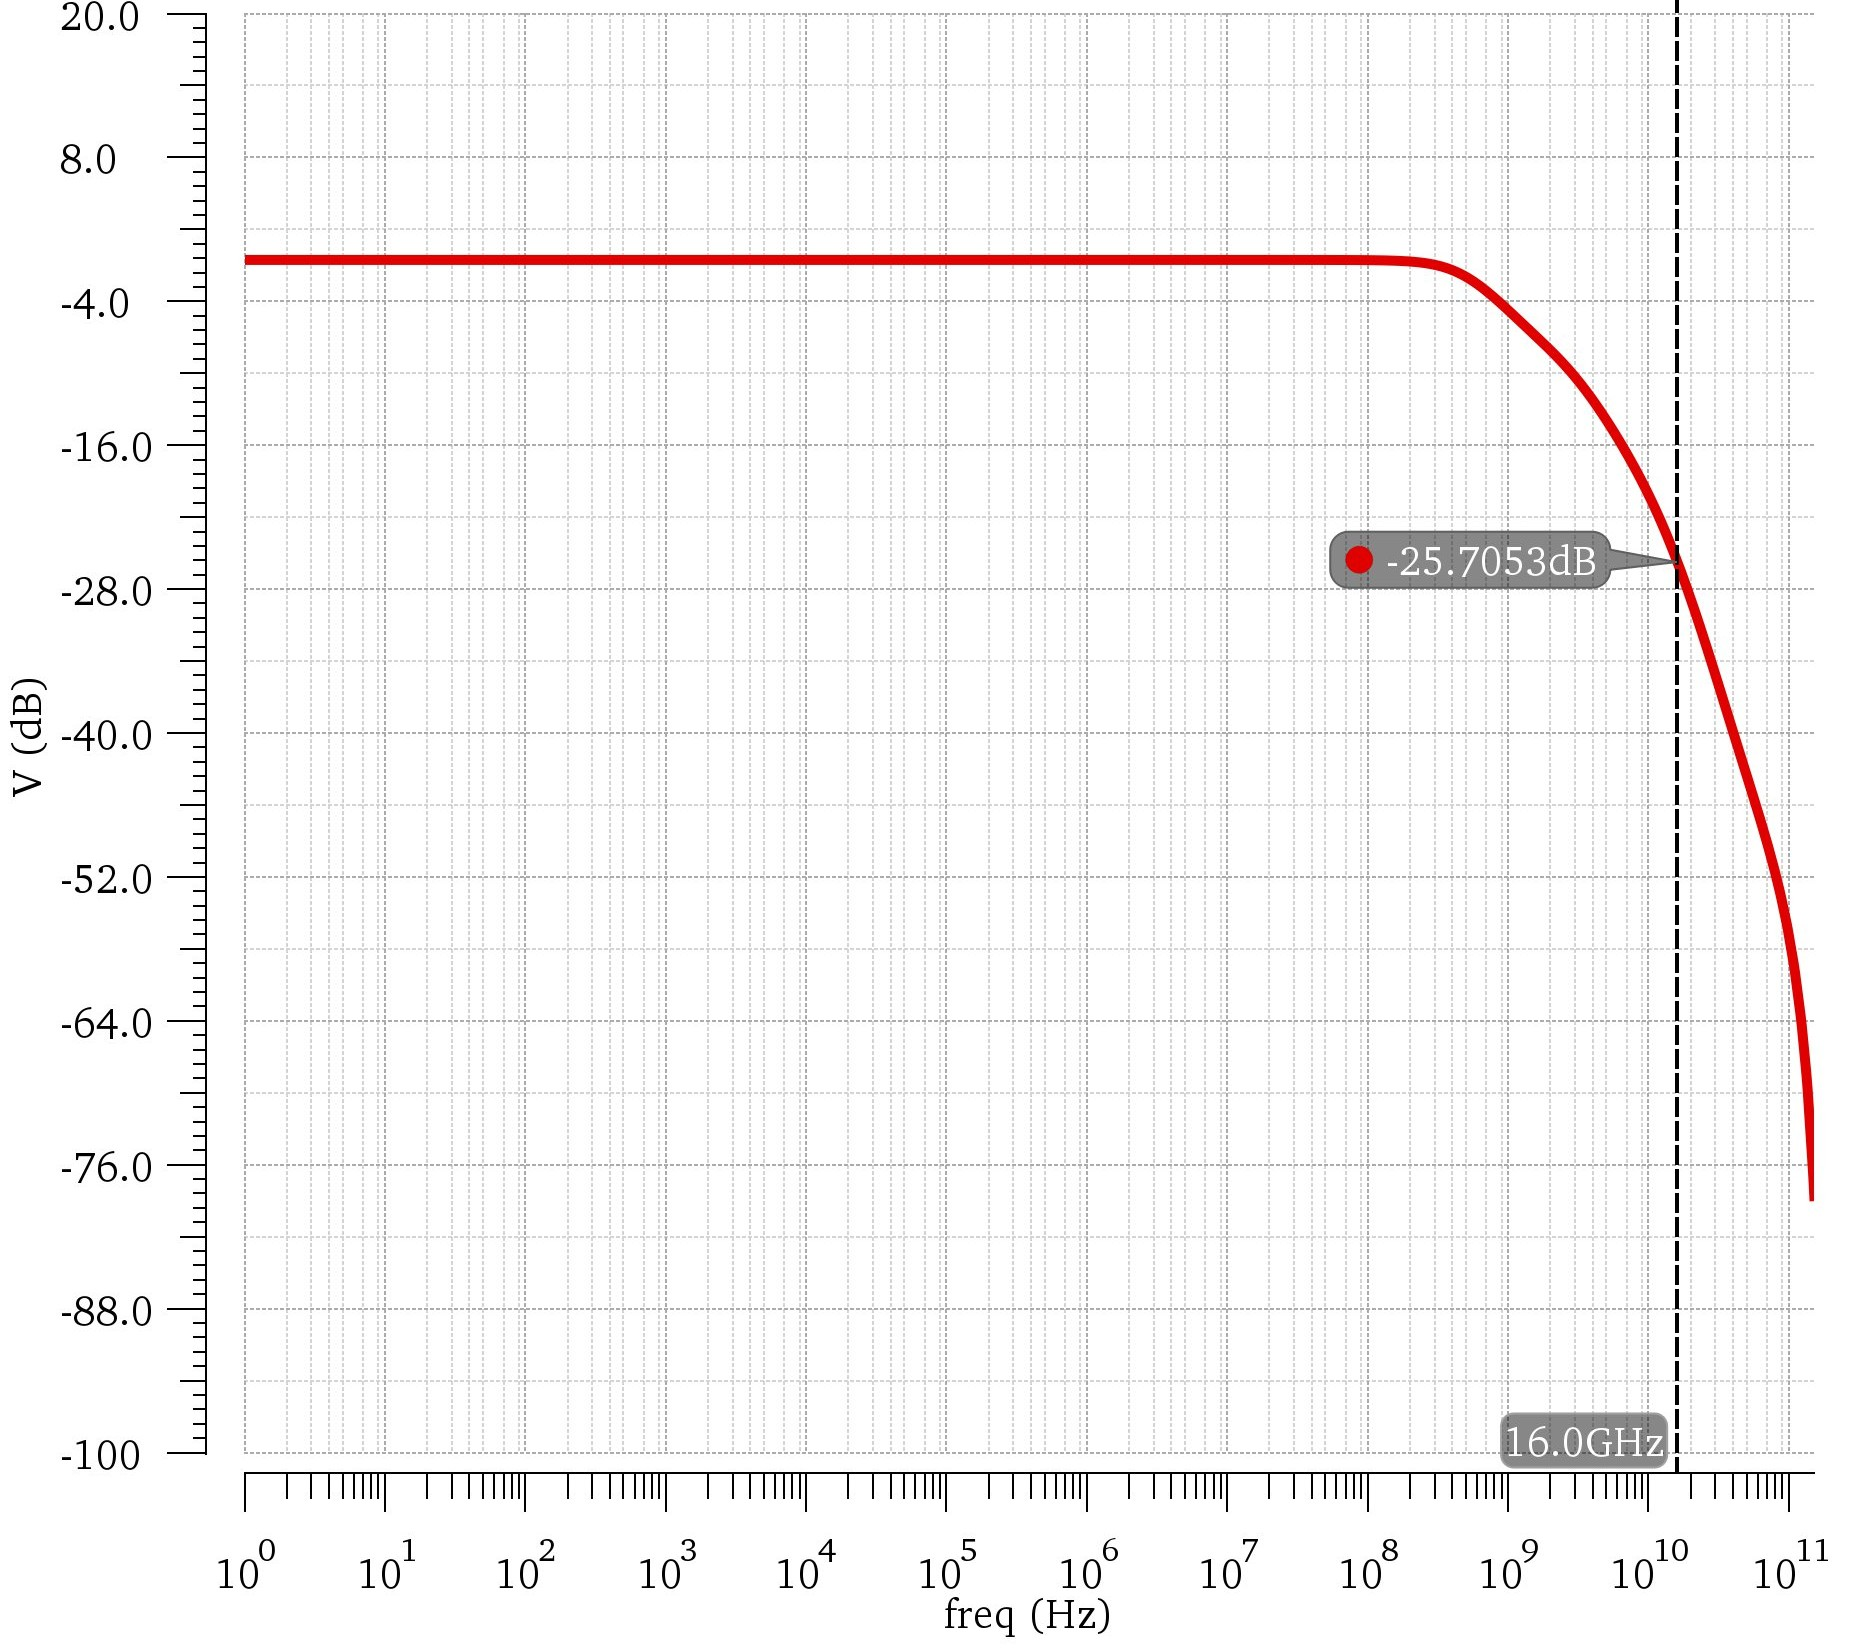
\includegraphics[width=0.65\textwidth]{img/CTLE_img/channel_response.jpg}
    \caption{Frequency response of the cascaded channel model, illustrating a severe insertion loss of approximately $-$26 dB at the Nyquist frequency.}
    \label{fig:channel_response}
\end{figure}

\noindent Before implementing the transistor-level design, \textbf{the behavioral CTLE was implemented in Verilog-A code}. Behavioral simulations were then conducted to observe the AC response of the CTLE and its interaction with this uncompensated $-$26 dB channel. Figure~\ref{fig:behavioral_ctle_curves} demonstrates the AC response of the behavioral model, sweeping through its various adjustable DC gain configurations to provide different levels of peaking.

\begin{figure}[H]
    \centering
    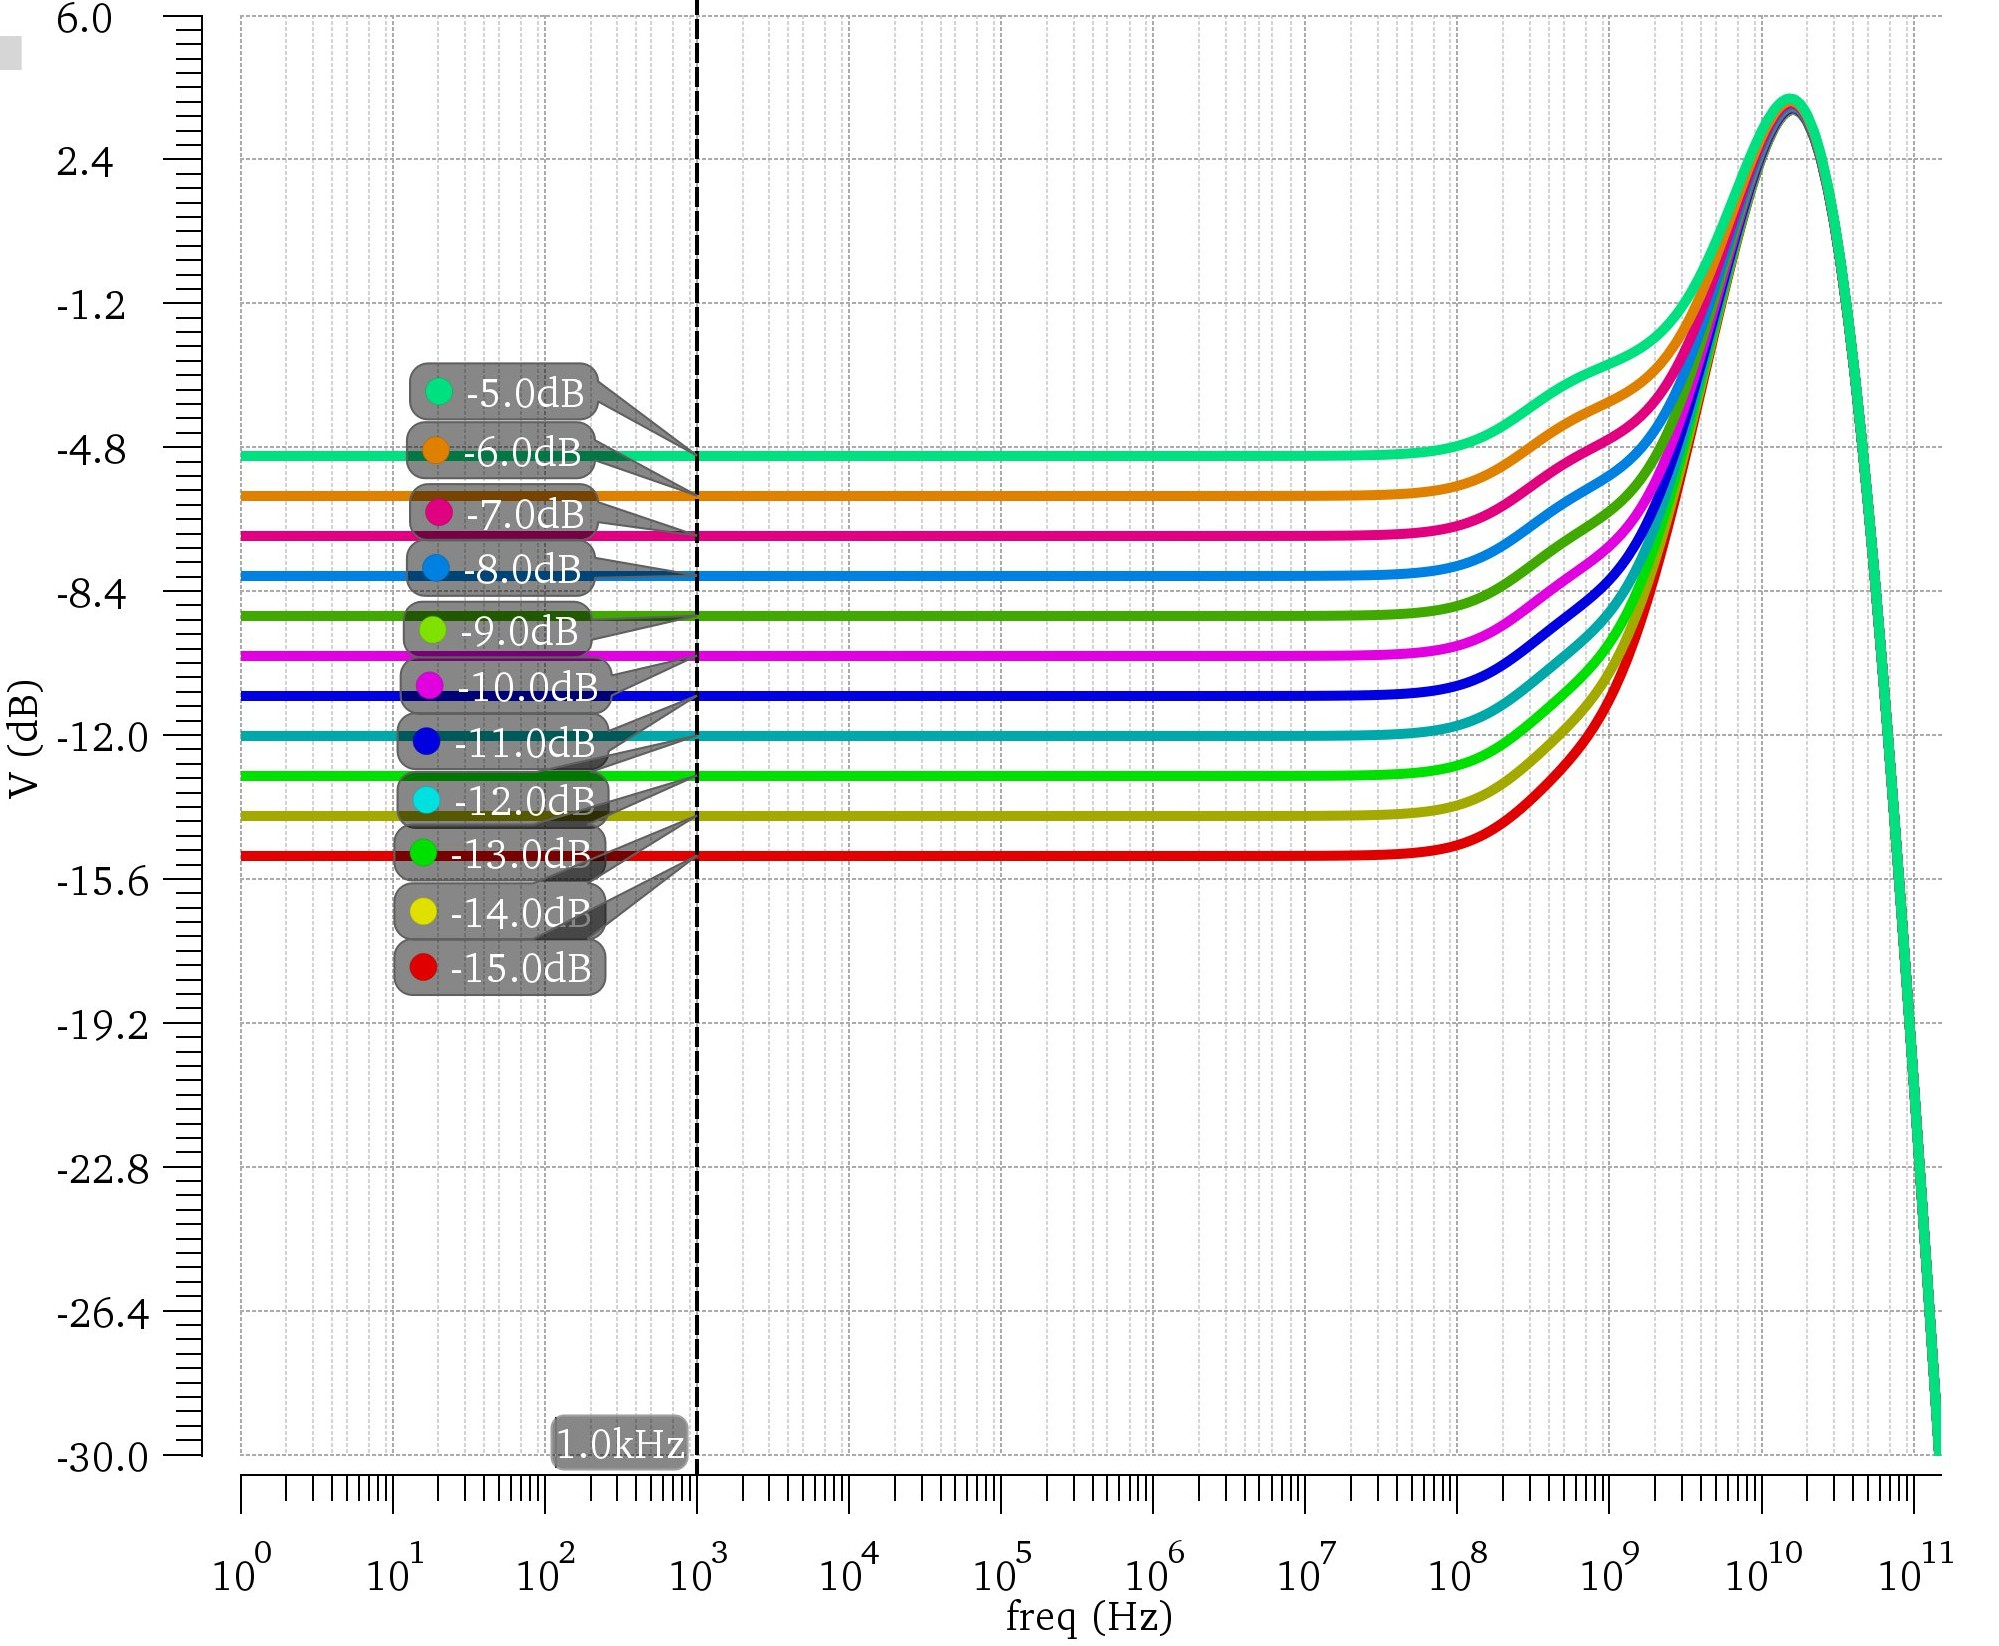
\includegraphics[width=0.85\textwidth]{img/CTLE_img/behavioral_ctle_response.jpg}
    \caption{Behavioral CTLE simulation showing the AC response curves across various DC gain configurations.}
    \label{fig:behavioral_ctle_curves}
\end{figure}

\noindent The simulation setup utilizes a Pseudorandom Binary Sequence (PRBS). For the behavioral tests, an Linear Feedback Shift Register (LFSR) mode of PN13 was utilized as the primary stimulus. The bit period is defined as 1 Unit Interval (UI), and realistic signal transitions were modeled with both rise time and fall time configured to 0.1 UI.\\

\noindent By tuning the CTLE's DC gain and zero locations, the high-frequency peaking is configured to invert the channel's $-$26 dB attenuation profile. When this equalization is mathematically superimposed over the channel response, the resulting total transfer function demonstrates a significantly flattened magnitude across the frequency band of interest, successfully verifying the theoretical limits of the 6-pole, 3-zero model.

\section*{Transient Simulation and PAM4 Eye Recovery}
Because PCIe 6.0 utilizes Pulse Amplitude Modulation 4-level (PAM4) signaling to achieve the 64 GT/s data rate, the equalizer must clearly resolve three distinct data eyes. Signal integrity is measured by evaluating these eye openings post-equalization.

\begin{figure}[H]
    \centering
    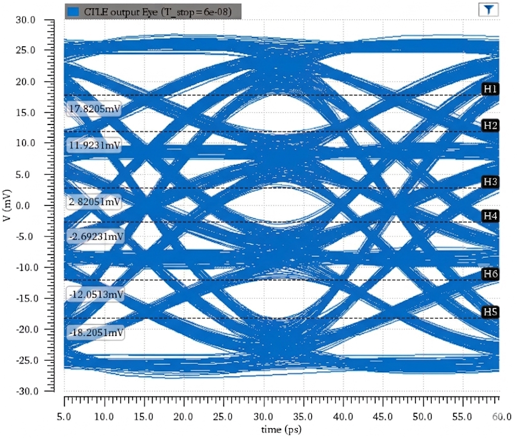
\includegraphics[width=0.85\textwidth]{img/CTLE_img/behavioral_CTLE_AC_eye_diagram_19db_channel.png}
    \caption{Post-CTLE Behavioral Eye Diagram at 64 GT/s. The equalization successfully recovers the three distinct PAM4 eyes after passing through the physical channel.}
    \label{fig:eye_diagram}
\end{figure}

\noindent Figure~\ref{fig:eye_diagram} presents the CTLE output eye diagram captured during the transient simulation. The effectiveness of the behavioral model is evidenced by the distinct separation of the PAM4 levels despite the severe channel attenuation. The eye diagram explicitly maps the critical crossing thresholds, verifying that the multi-pole shaping adequately minimizes ISI and restores the required amplitude limits for the downstream slicers. \\

\noindent Establishing this behavioral baseline proves that the architecture can mathematically satisfy the PCIe 6.0 standard under extreme loss conditions, allowing the design focus to shift toward realizing these exact poles, zeros, and gain steps using a physical, transistor-level analog front-end topology.


\subsection{Topology Selection and Proposed Architecture}

\section*{Initial Approach: Single-Stage SD CTLE}

During the initial design phase, a conventional single-stage Source-Degenerated (SD) CTLE was evaluated. However, testing this topology against the severe PCIe 6.0 channel model revealed two critical limitations, which are clearly evident when compared to the target behavioral model in Figure~\ref{fig:sd_vs_behav_response}:

\begin{enumerate}
    \item \textbf{Insufficient Gain Boost:} A single stage fundamentally lacks the capability to achieve the aggressive \textbf{19 dB} maximum high-frequency peaking mandated by the standard without pushing transistors into non-linear regions or consuming excessive power.
    \item \textbf{Lack of Mid-Band Compensation:} A conventional SD CTLE provides only a single high-frequency zero. Equalizing a complex, multi-pole channel roll-off with a single zero leaves a pronounced mid-band droop that severely distorts PAM4 eye transitions.
\end{enumerate}

\begin{figure}[H]
    \centering
    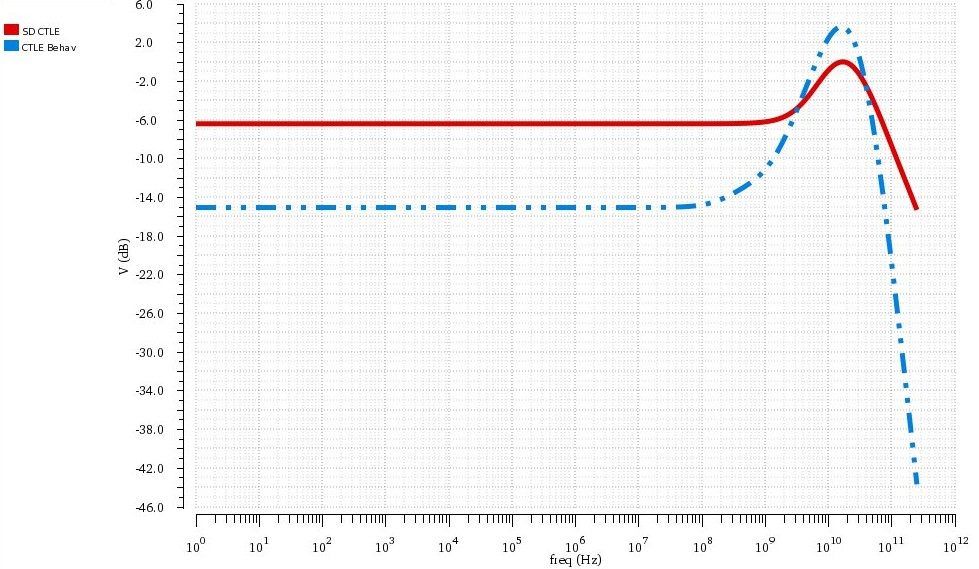
\includegraphics[width=0.85\textwidth]{img/CTLE_img/only_onestage_SD_ctle.jpg}
    \caption{AC response of a single-stage SD CTLE compared with the behavioral model.}
    \label{fig:sd_vs_behav_response}
\end{figure}

\noindent To resolve these performance deficits, the architecture must cascade an additional stage to introduce more poles and zeros, providing the necessary degrees of freedom to tune the response and reach the total required boost. Furthermore, addressing the mid-band attenuation requires a specialized architectural adjustment: by introducing a parallel low-pass path ($G_{m2}$) into the primary stage, the mid-band droop is effectively lifted, creating a smooth, fully compensated equalization profile.

\section*{Proposed Two-Stage Topology}

To overcome the gain and mid-band limitations of the single-stage approach, a two-stage cascaded architecture was developed. As illustrated in Figure~\ref{fig:proposed_topology_block}, the proposed implementation adopts the following cascade:

\begin{figure}[H]
    \centering
    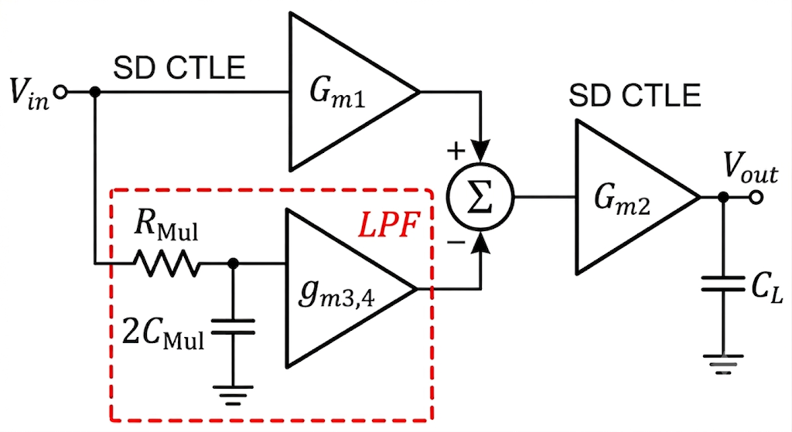
\includegraphics[width=0.7\textwidth]{img/CTLE_img/proposed_topology_block_diagram.png}
    \caption{Block-level diagram of the proposed two-stage CTLE: Stage 1 (Dual-path CTLE) followed by Stage 2 (SD CTLE).}
    \label{fig:proposed_topology_block}
\end{figure}

\begin{enumerate}[noitemsep]
\item \textbf{Stage 1 — Two-Path CTLE:} An SD CTLE augmented with a low-pass $g_m$ branch to compensate for mid-band droop through an additional zero.
\item \textbf{Stage 2 — SD CTLE:} A conventional SD stage that adds a pole/zero pair, increasing high-frequency peaking to reach the \textbf{19 dB} target.
\end{enumerate}

\noindent This cascade provides \textbf{five poles and three zeros}, closely approximating the PCIe 6.0 behavioral reference. The schematic is shown in Figure~\ref{fig:proposed_topology_schematic}.

\begin{figure}[H]
    \centering
    \includegraphics[width=\textwidth]{img/CTLE_img/proposed_topology.png}
    \caption{Transistor-level schematic of the proposed Two-Path + SD CTLE cascaded topology.}
    \label{fig:proposed_topology_schematic}
\end{figure}

\subsection*{Transfer Function}

The overall transfer function of the first stage (Two-path CTLE) is defined by the summation of the main SD path and the secondary low-pass path, given by:

\begin{equation*}
    H_1(s) \simeq -\!\left(\frac{g_{m1,2}}{1+\dfrac{g_{m1,2}R_S}{2}}
    - g_{m3,4}\right)R_L \cdot
    \frac{\left(1+\dfrac{s}{\omega_z}\right)
          \left(1+\dfrac{s}{\omega_{z\_\mathrm{Lpf}}}\right)}
         {\left(1+\dfrac{s}{\omega_{p1}}\right)
          \left(1+\dfrac{s}{\omega_{p2}}\right)
          \left(1+\dfrac{s}{\omega_{p\_\mathrm{Lpf}}}\right)}
    \label{eq:H2}
\end{equation*}

\noindent where the dominant poles and zeros of the main SD path are defined as:
\begin{align*}
    \omega_z       &= \frac{1}{R_S C_S},   \quad
    \omega_{p1}    = \frac{1+g_m R_S/2}{R_S C_S}, \quad
    \omega_{p2}    = \frac{1}{R_L C_L}     \label{eq:poles_sd}
\end{align*}

\noindent and the supplementary mid-band pole and zero introduced by the dual path ($g_{m3,4}$) branch are:
\begin{align*}
    \omega_{z\_\mathrm{Mul}} &= \frac{g_{m1,2}-g_{m3,4}\!\left(1+\frac{g_{m1,2}R_s}{2}\right)}
                                    {2\,g_{m1,2}\,R_{\mathrm{Lpf}}\,C_{\mathrm{Lpf}}},
    \quad
    \omega_{p\_\mathrm{Lpf}} = \frac{1}{2\,R_{\mathrm{Lpf}}\,C_{\mathrm{Lpf}}}
\end{align*}

\noindent The full composite transfer function is given by:

\begin{equation*}
    H_{total}(s) = H_1(s) \cdot H_2(s)
\end{equation*}

\begin{equation*}
    H_{total}(s) = \underbrace{\left[ A_{DC,1} \cdot \frac{(1+\frac{s}{\omega_z})(1+\frac{s}{\omega_{z\_\mathrm{Lpf}}})}{(1+\frac{s}{\omega_{p1}})(1+\frac{s}{\omega_{p2}})(1+\frac{s}{\omega_{p\_\mathrm{Lpf}}})} \right]}_{H_1(s)} \cdot \underbrace{\left[ A_{DC,2} \cdot \frac{(1+\frac{s}{\omega_{z,SD2}})}{(1+\frac{s}{\omega_{p,SD2}})(1+\frac{s}{\omega_{p2,SD2}})} \right]}_{H_2(s)}
\end{equation*}

\begin{equation*}
    A_{DC,total} = -\left[ \left(\frac{g_{m1,2}}{1+\frac{g_{m1,2}R_S}{2}} - g_{m3,4}\right)R_L \right] \cdot \left[ \frac{g_{m,SD2}}{1+\frac{g_{m,SD2}R_{S,SD2}}{2}} R_{L,SD2} \right]
\end{equation*} 
\newline

\noindent Cascading the second SD CTLE stage appends one additional zero ($\omega_z$) and two additional poles ($\omega_{p1}$, $\omega_{p2}$), resulting in the highly tunable five-pole, three-zero composite response required to recover the 64.0 GT/s signal.


\section*{Circuit Design and Analysis}

\subsection{Full Circuit Schematic}

Figure~\ref{fig:full_schematic} displays the complete annotated schematic of the two-stage CTLE, including all back-annotated parasitics. The design utilizes 22\,nm SOI Super-Low VT (SLVT) transistors (\texttt{slvtnfet\_mmw\_5t}) throughout. To model layout interconnects, all signal traces include grey-model back-annotations of $4\,\Omega$ per resistive segment and $5\,\text{fF}$ per capacitive node.

\begin{figure}[H]
    \centering
    \includegraphics[width=\textwidth]{img/CTLE_img/Circuit_schematic_with_back_annotations.png}
    \caption{Complete annotated schematic of the proposed two-stage CTLE with back-annotated device dimensions and parasitics.}
    \label{fig:full_schematic}
\end{figure}

\subsection*{Stage 1: Dual Path Source-Degenerated CTLE}

The first stage provides the primary tunability for the system. It consists of a high-swing SD CTLE core path augmented with a low-pass multi-path (LPF+$G_{m2}$) branch to flatten mid-band gain.

\subsubsection*{Core Differential Pair and Load ($G_{m1}$)}
The input differential pair ($N_1, N_2$) is sized at $20\,\mu\text{m}/20\,\text{n}\text{m}$, biased by tail current sources ($N_7, N_8$) sized at $40\,\mu\text{m}/100\,\text{n}\text{m}$. The stage utilizes N+ polysilicon load resistors (\texttt{opnpc}) with a value of $145.7\,\Omega$ ($7\,\mu\text{m} \times 2\,\mu\text{m}$ sizing).

\newpage
\subsubsection*{Multi-Path Branch (LPF + Gm cell)}
The secondary low-pass branch ($N_3, N_4$) is sized at $2.4\,\mu\text{m}/20\,\text{n}\text{m}$ with a tail current source ($N_9$) sized at $10\,\mu\text{m}/100\,\text{n}\text{m}$. The branch filter is composed of a $500\,\Omega$ \texttt{opnpc} resistor and an \texttt{apmom} capacitor of $200\,\text{fF}$ ($9\,\mu\text{m} \times 9\,\mu\text{m}$), which sets the mid-band correction frequency. 

\subsubsection*{Tunability}
All DC gain and equalization peaking tunability is centralized in this stage via a programmable resistor bank and capacitive bank, allowing dynamic adjustment of the $R_S-C_S$ degeneration network.

\subsection*{Stage 2: Fixed SD CTLE}

The second stage is a fixed, non-tunable SD CTLE designed for high-frequency boost. To simplify layout, it is architected as a symmetric half-cell, allowing for a mirrored layout implementation.

\subsubsection*{Core Pair and Load}
The input pair ($N_5, N_6$) is sized at $20\,\mu\text{m}/100\,\text{n}\text{m}$ with tail current sources ($40\,\mu\text{m}/100\,\text{n}\text{m}$). The load resistors are $240\,\Omega$ \texttt{opnpc} ($4.26\,\mu\text{m} \times 2\,\mu\text{m}$).

\subsubsection*{Degeneration Network}
The degeneration network for this stage is fixed and utilizes high-precision \texttt{apmom} and \texttt{opnpc} elements:
\begin{itemize}[noitemsep]
    \item \textbf{Resistors:} Two series identical \texttt{opnpc} resistors, each $351\,\Omega$ ($2.9\,\mu\text{m} \times 2\,\mu\text{m}$).
    \item \textbf{Capacitors:} Two parallel \texttt{apmom} capacitors, each $32\,\text{fF}$ ($3.7\,\mu\text{m} \times 3.7\,\mu\text{m}$).
\end{itemize}

\newpage
\subsection{Thermometer-Coded Resistive Degeneration Bank}
\label{sec:rbank}

The DC gain of the CTLE is controlled by varying the effective source-degeneration resistance $R_S$ using a thermometer-coded resistive bank. As shown in Figure~\ref{fig:rbank}, this bank utilizes a set of parallel branches, each controlled by the digital thermometer bus $r\langle9:0\rangle$.

\begin{figure}[H]
    \centering
    \includegraphics[width=0.8\textwidth]{img/CTLE_img/Resistor_bank_schematic.png}
    \caption{Schematic of the thermometer-coded degeneration resistive bank used for DC gain control and PVT compensation.}
    \label{fig:rbank}
\end{figure}

\subsection*{Gain Control Logic}
The bank operates by selectively activating parallel branches to adjust the total degeneration resistance $R_S$, which in turn controls the DC gain and peaking according to:
\begin{equation*}
    A_{\mathrm{DC}} \approx \frac{g_{m1,2}\,R_L}{1+g_{m1,2}R_S/2},
    \qquad
    \mathrm{Boost} = 1 + \frac{g_m R_S}{2}
\end{equation*}

\noindent The bank includes PVT compensation via control signals $R_1$ and $R_2$, which are gate signals for switches placed in parallel with specific degeneration resistors. When a gate signal (e.g., $R_1$ or $R_2$) is asserted (HIGH), the respective switch is turned ON, shorting the resistor in parallel with it.
\newpage Each switch is designed with an on-resistance ($R_{on}$) of approximately $10\,\Omega$, which is accounted for in the effective resistance when a branch is active.

The gain control follows a structured activation sequence:
\begin{itemize}
    \item \textbf{-15 dB (Minimum Gain/ Max Peaking):} All parallel branches controlled by $r\langle9:0\rangle$ are disabled. The degeneration is provided solely by the "always-active" branch, which contains two series resistors without an associated switch.
    \item \textbf{-14 dB:} Only $r\langle9\rangle$ is activated, placing its branch in parallel with the always-active branch.
    \item \textbf{-13 dB:} $r\langle9\rangle$ and $r\langle8\rangle$ are activated in parallel.
    \item \textbf{-12 dB:} $r\langle9\rangle$, $r\langle8\rangle$, and $r\langle7\rangle$ are activated.
    \item[] \hfil$\vdots$\hfil
    \item \textbf{-5 dB (Maximum Gain/ Min Peaking):} All parallel branches are active, providing minimum degeneration.
\end{itemize}
This thermometer-coded approach ensures monotonic gain steps and prevents transient glitches during state transitions.

\subsection*{PVT Corner Compensation}
To maintain consistent performance across PVT corners, two fixed resistors, $R_1$ and $R_2$, are incorporated to compensate for resistance degradation:
\begin{itemize}
    \item \textbf{$R_2$:} This resistor is permanently included in all Fast-Fast (FF) corners to prevent excessive gain due to increased transistor mobility and lower effective resistance values.
    \item \textbf{$R_1$:} This resistor is selectively engaged only in the FF125$^{\circ}$C ($-5\% V_{DD}$) corner to provide additional degeneration, counteracting the gain increase and maintaining the target equalization profile.
\end{itemize}


\newpage
\subsection{Capacitive Degeneration Bank}
\label{sec:capbank}

The capacitive degeneration bank tunes the zero frequency ($\omega_z = 1/R_S C_S$) to stabilize the CTLE peaking profile across process, voltage, and temperature (PVT) variations. As shown in Figure~\ref{fig:cap_bank}, the bank uses calibration signals \texttt{calib0} and \texttt{calib1} to adjust the total effective degeneration capacitance ($C_S$).

\begin{figure}[H]
    \centering
    \includegraphics[width=0.7\textwidth]{img/CTLE_img/cap_bank.png}
    \caption{Capacitive degeneration bank schematic using \texttt{calib0} and \texttt{calib1} for PVT-dependent peaking adjustment.}
    \label{fig:cap_bank}
\end{figure}

\subsection*{Principle of Operation}
The network defaults to a base capacitance when \texttt{calib0} and \texttt{calib1} are inactive. Asserting these signals closes the respective switches, adding capacitors in parallel to $C_S$. This tunability compensates for process-induced shifts in transconductance ($g_m$):

\begin{itemize}
    \item \textbf{Typical-Typical (TT) Corner (\texttt{calib0}=VDD, \texttt{calib1}=0):} Sets the nominal capacitive load.
    \item \textbf{Fast-Fast (FF) Corner (\texttt{calib0}=VDD, \texttt{calib1}=VDD):} Higher mobility increases intrinsic peaking. Adding capacitance shifts $\omega_z$ lower, dampening excessive high-frequency gain to restore the target profile.
    \item \textbf{Slow-Slow (SS) Corner (\texttt{calib0}=0, \texttt{calib1}=0):} Lower mobility degrades peaking. Minimizing $C_S$ shifts $\omega_z$ higher, reducing high-frequency degeneration to recover the necessary gain boost.
\end{itemize}

By dynamically adjusting $C_S$, the bank centers the CTLE peaking at the Nyquist frequency, decoupling the equalization magnitude from process-dependent $g_m$ variations.

\subsection{Biasing Network}
\label{sec:bias}

The biasing network is responsible for generating the stable gate bias voltages ($V_{\mathrm{bs1}}$ and $V_{\mathrm{bs2}}$) required by the CTLE tail current sources. To ensure robust equalization performance across all PVT corners, the network utilizes a digitally controlled, custom-weighted current DAC (I-DAC) architecture that regulates the nominal $1.05\,\text{mA}$ reference current.

Figure~\ref{fig:bias_schematic} illustrates the complete top-level schematic of the I-DAC, highlighting the current-steering network divided into parallel weighted branches to provide high-resolution dynamic range.

\begin{figure}[H]
    \centering
    \includegraphics[width=0.95\textwidth]{img/CTLE_img/bias_schematic.png}
    \caption{Biasing network schematic featuring the custom-weighted I-DAC architecture. The network utilizes parallel branches with specific fractional weights of the reference current.}
    \label{fig:bias_schematic}
\end{figure}

\subsection*{Principle of Operation and Custom Weighting}
The I-DAC provides the necessary dynamic range to actively counteract PVT-induced variations in the equalizer's transconductance ($g_m$). The total reference current is distributed across four distinct, precisely weighted branches:
\begin{itemize}[noitemsep]
    \item \textbf{Base Branch (Always-On):} A fixed branch provides a minimum of $60\%$ of the reference current, ensuring the CTLE maintains a stable baseline operation under all conditions (e.g., preventing complete shut-off during extreme Slow-Slow corners).
    \item \textbf{V3 Control Branch ($40\%$):} Controlled by digital signal V3, supplying $40\%$ of the nominal current.
    \item \textbf{V1 Control Branch ($20\%$):} Controlled by digital signal V1, supplying $20\%$ of the nominal current.
    \item \textbf{V2 Control Branch ($80\%$):} Controlled by digital signal V2, supplying $80\%$ of the nominal current.
\end{itemize}

By asserting the appropriate combination of the V1, V2, and V3 control bits, the total bias current can be scaled from a minimum of $60\%$ up to a maximum of $200\%$ of the nominal value. This wide programmable range is heavily utilized in Fast-Fast (FF) corners to scale up the current and compensate for mobility-driven performance shifts, while allowing selective deactivation in Slow-Slow (SS) corners to prevent the bias current from exceeding target margins and causing excessive gain.

\subsection*{2-Way Branch Switching Mechanism}
To cleanly activate and deactivate the dynamically weighted branches without disturbing the primary reference diode, a custom 2-way switch topology is implemented, as detailed in Figure~\ref{fig:bias_switch}.

\begin{figure}[H]
    \centering
    \includegraphics[width=0.50\textwidth]{img/CTLE_img/2way_switch.png}
    \caption{Schematic of the 2-way switch topology used to activate or deactivate the individual weighted PMOS current mirror branches.}
    \label{fig:bias_switch}
\end{figure}

When a specific branch is disabled by its digital control signal ($V_{\text{ctrl}}$), the 2-way switch actively pulls the gate voltage of that branch's PMOS mirror device directly to $V_{\mathrm{DD}}$. This entirely shuts off the transistor, eliminating sub-threshold leakage. Conversely, when enabled, the switch seamlessly connects the gate to the primary diode-connected control voltage ($V_G$), allowing the branch to accurately mirror its designated fractional current.

\subsection*{Multi-Stage Mirroring}
The network employs five primary PMOS mirrors ($30\,\mu\text{m}/100\,\text{n}\text{m}$) and utilizes minimum-sized devices ($2.4\,\mu\text{m}/20\,\text{n}\text{m}$) for the 2-way control switches to minimize parasitic gate capacitance. To support the low-pass filter (LPF) branch's substantially lower current requirement of $70\,\mu\text{A}$, a secondary local NMOS mirror is implemented. This secondary mirror scales the primary $1.05\,\text{mA}$ reference down to the exact $70\,\mu\text{A}$ required. This hierarchical biasing strategy completely avoids the immense silicon area overhead that would otherwise be required by utilizing excessive high-ratio current multipliers, while effectively stabilizing the CTLE's $g_m$ and peaking frequency across all operating corners.

\newpage
\subsection*{Testbench}
\label{sec:tb}

To validate the two-stage CTLE, a testbench was developed to emulate the severe PCIe 6.0 channel insertion loss. The setup integrates the transistor-level design with bias circuitry, calibration banks, and a thermometer decoder, which generates the control signals for the resistive bank.

\begin{figure}[H]
    \centering
    \includegraphics[width=\textwidth]{img/CTLE_img/ctle_test_bench.png}
    \caption{CTLE simulation testbench with thermometer-coded gain control.}
    \label{fig:ctle_testbench}
\end{figure}

\subsection*{Simulation Methodology}
The environment performs the following analyses:
\begin{itemize}[noitemsep]
    \item \textbf{AC Analysis:} Measures frequency response, peaking magnitude, and mid-band compensation effectiveness.
    \item \textbf{PVT Corner Analysis:} Evaluates gain and calibration robustness across FF, SS, and TT corners to ensure stable equalization under extreme conditions.
    \item \textbf{Transient Analysis:} Assesses 64.0\,GT/s signal integrity. The input includes the PCIe 6.0 channel and matching network to confirm the suppression of inter-symbol interference (ISI).
\end{itemize}

\noindent This testbench optimized the design to meet the aggressive \textbf{19 dB} high-frequency boost requirement while maintaining linearity within the 22\,nm SOI process.



\subsection{Simulation Results}
\label{sec:sim_results}

This section details the comprehensive pre-layout simulation results for the proposed two-stage Continuous-Time Linear Equalizer (CTLE). To thoroughly evaluate the design, all simulations were executed within the Cadence Spectre environment utilizing a 22\,nm SOI process technology design kit. Unless otherwise specified, the testing environment assumed a nominal supply voltage of 0.8\,V and an input common-mode voltage ($V_{\mathrm{ICM}}$) of 540\,mV. 

\subsection*{AC Response — Maximum Boost Setting (DC Gain = -15\,dB)}

Figure~\ref{fig:ac_response_2_stages} illustrates the AC frequency response of the equalizer configured at its maximum boost setting, which corresponds to a DC gain of -15\,dB. To provide insight into the distributed equalization strategy, the individual frequency responses of Stage~1 and Stage~2 are plotted independently alongside the cascaded total CTLE response. A behavioral reference model is also superimposed to confirm that the transistor-level implementation accurately tracks the ideal target profile.

\begin{figure}[H]
    \centering
    \includegraphics[width=0.90\textwidth]{img/CTLE_img/ac_response_2_stages.png}
    \caption{AC frequency response evaluated at DC gain = -15\,dB ($V_{\mathrm{ICM}} = 540$\,mV).}
    \label{fig:ac_response_2_stages}
\end{figure}

\noindent The key performance metrics extracted from this maximum boost configuration are summarized as follows:
\begin{itemize}[noitemsep]
    \item \textbf{Total DC Gain:} -15.0\,dB
    \item \textbf{Individual Stage DC Gain:} Stage~1 contributes -8.69\,dB; Stage~2 contributes -6.28\,dB.
    \item \textbf{Gain at Nyquist Frequency (16\,GHz):} Peaking achieves between +3.42\,dB and +3.65\,dB.
    \item \textbf{High-Frequency (HF) Boost:} The total effective boost from DC to the Nyquist frequency is approximately 19\,dB.
\end{itemize}

\subsubsection{AC Simulation Across All Gain Settings}

To verify the tunability of the mid-band and low-frequency attenuation, Figure~\ref{fig:ac_response_2_stages_all_settings} presents the cascaded CTLE frequency response across all eleven discrete gain settings. The DC gain is swept from its maximum value of -5\,dB down to its minimum value of -15\,dB, with the measured DC gain annotated directly on each corresponding curve.

\begin{figure}[H]
    \centering
    \includegraphics[width=0.90\textwidth]{img/CTLE_img/ac_response_2_stages_all_settings.png}
    \caption{Family of AC frequency response curves representing all eleven DC gain control settings.}
    \label{fig:ac_response_2_stages_all_settings}
\end{figure}

\noindent The operation of the thermometer-coded resistive degeneration bank ensures that the gain steps are highly uniform. The design achieves monotonic steps of approximately 1\,dB throughout the entire control range. The precise measured DC gain for each digital control word is documented in Table~\ref{tab:dc_gain_values}.

\begin{table}[H]
    \centering
    \caption{Measured low-frequency DC gain values for all eleven programmable gain control settings.}
    \label{tab:dc_gain_values}
    \begin{tabular}{cc|cc}
        \toprule
        \textbf{DC\_Ctrl} & \textbf{DC Gain (dB)} & \textbf{DC\_Ctrl} & \textbf{DC Gain (dB)} \\
        \midrule
        5  & $-4.995$  & 11 & $-11.045$ \\
        6  & $-6.006$  & 12 & $-12.010$ \\
        7  & $-6.999$  & 13 & $-13.048$ \\
        8  & $-7.995$  & 14 & $-13.960$ \\
        9  & $-9.003$  & 15 & $-15.045$ \\
        10 & $-10.006$ &    &           \\
        \bottomrule
    \end{tabular}
\end{table}

\subsubsection*{Input and Output Swing — Linearity Analysis}
Maintaining signal linearity is critical to prevent the equalizer from introducing harmonic distortion into the data stream. Linearity was analyzed by sweeping the differential input amplitude and measuring the fundamental harmonic of the output signal.

\subsubsection*{High Boost Setting (DC Gain = -15\,dB)}
Figure~\ref{fig:ctle_gain_linearity_gain_15dB_1db_compression} evaluates the CTLE gain linearity at the highest boost setting, using a 1\,kHz test tone with a baseline differential input of 0.5\,V$_{\text{pp,diff}}$. The corresponding time-domain waveforms are shown in Figure~\ref{fig:ctle_gain_linearity_gain_15dB_sinwave}.

\begin{figure}[H]
    \centering
    \includegraphics[width=0.8\textwidth]{img/CTLE_img/ctle_gain_linearity_gain_15dB_1db_compression.png}
    \caption{CTLE gain linearity characteristics (output fundamental amplitude versus input amplitude) configured at DC gain = -15\,dB.}
    \label{fig:ctle_gain_linearity_gain_15dB_1db_compression}
\end{figure}

\begin{figure}[H]
    \centering
    \includegraphics[width=0.8\textwidth]{img/CTLE_img/ctle_gain_linearity_gain_15dB_sinwave.png}
    \caption{Time-domain waveforms at DC gain = -15\,dB, illustrating the input and output voltage swings.}
    \label{fig:ctle_gain_linearity_gain_15dB_sinwave}
\end{figure}

The extracted linearity parameters at the maximum boost configuration are:
\begin{itemize}[noitemsep, topsep=0pt]
    \item \textbf{1-dB Compression Point:} Reached at an input of 552.1\,mV, corresponding to an output of 106.0\,mV.
    \item \textbf{Linear Input Range:} The circuit maintains a linear response up to approximately 1.1\,V$_{\text{pp,diff}}$.
    \item \textbf{Output Swing:} The available linear output swing is approximately 210\,mV$_{\text{pp,diff}}$.
\end{itemize}

\subsubsection*{Low Boost Setting (DC Gain = -5\,dB)}

Figure~\ref{fig:ctle_gain_linearity_gain_5dB_1db_compression} repeats this linearity characterization, configuring the equalizer to its minimum boost setting (maximum DC gain). The corresponding time-domain waveforms are shown in Figure~\ref{fig:ctle_gain_linearity_gain_5dB_sinwave}.

\begin{figure}[H]
    \centering
    \includegraphics[width=0.75\textwidth]{img/CTLE_img/ctle_gain_linearity_gain_5dB_1db_compression.png}
    \caption{CTLE gain linearity characteristics evaluated at DC gain = -5\,dB.}
    \label{fig:ctle_gain_linearity_gain_5dB_1db_compression}
\end{figure}

\begin{figure}[H]
    \centering
    \includegraphics[width=0.75\textwidth]{img/CTLE_img/ctle_gain_linearity_gain_5dB_sinwave.png}
    \caption{Time-domain waveforms at DC gain = -5\,dB, illustrating the input and output voltage swings.}
    \label{fig:ctle_gain_linearity_gain_5dB_sinwave}
\end{figure}

The extracted linearity parameters at the minimum boost configuration are:
\begin{itemize}[noitemsep]
    \item \textbf{1-dB Compression Point:} Reached earlier due to higher DC gain, occurring at an input of 333.2\,mV with an output of 106.0\,mV.
    \item \textbf{Linear Input Range:} The linear input boundary shifts to approximately 660\,mV$_{\text{pp,diff}}$.
    \item \textbf{Output Swing:} The available linear output swing remains steady at approximately 210\,mV$_{\text{pp,diff}}$.
\end{itemize}

\subsubsection{Noise Analysis}

Figure~\ref{fig:ctle_pnoise} details the simulated broad-spectrum output-referred noise spectral density of the CTLE. At lower frequencies, the noise profile is heavily dominated by flicker ($1/f$) noise. As the frequency increases beyond approximately $1\,\text{MHz}$, the profile transitions into a flat thermal noise floor. 

\begin{figure}[H]
    \centering
    \includegraphics[width=0.90\textwidth]{img/CTLE_img/ctle_pnoise.png}
    \caption{Broadband output-referred noise spectral density profile, highlighting the low-frequency flicker noise region and the transition to the thermal noise floor.}
    \label{fig:ctle_pnoise}
\end{figure}

Figure~\ref{fig:pnoise_peaking} provides a detailed view of the high-frequency spectrum. Importantly, the output noise is actively shaped by the CTLE's frequency response. Because the equalizer applies significant high-frequency voltage gain to compensate for channel insertion loss, it inherently amplifies the thermal noise contribution of the input differential pair. This noise shaping results in a prominent spectral peak in the vicinity of the $16\,\text{GHz}$ Nyquist frequency.



\begin{figure}[H]
    \centering
    \includegraphics[width=0.90\textwidth]{img/CTLE_img/pnoise_peaking.png}
    \caption{High-frequency noise spectral density demonstrating thermal noise \\ shaping by the CTLE gain profile, with a distinct peak near the Nyquist frequency.}
    \label{fig:pnoise_peaking}
\end{figure}

The key quantitative noise measurements are summarized below:
\begin{itemize}[]
    \item \textbf{Total Output-Referred Noise (TT Corner):} The integrated noise across the bandwidth under nominal conditions is $682.1\,\mu\text{V}_{\text{rms}}$.
    \item \textbf{Total Output-Referred Noise (Worst Corner):} The integrated noise increases to a maximum of $767.6\,\mu\text{V}_{\text{rms}}$ under worst-case PVT conditions.
\end{itemize}

\newpage
\subsubsection{Transient Simulation — Single-Bit Response}
To evaluate the time-domain equalization performance, a transient single-bit response (SBR) simulation was executed using a severe $-26$\,dB insertion loss channel model with the equalizer set to a DC gain of $-15$\,dB. The SBR is plotted in Figure~\ref{fig:ctle_sbr} as normalized amplitude against the tap index $k$, where one tap interval corresponds to the Nyquist period ($T_{\mathrm{Nyq}} = 32.5$\,ps). The equalized CTLE output (red) features a sharp main cursor at $k=0$ and rapidly decaying post-cursor ISI, contrasting with the broad, slowly decaying un-equalized channel response (gold).

\begin{figure}[H]
    \centering
    \includegraphics[width=\textwidth]{img/CTLE_img/ctle_sbr.png}
    \caption{Single-bit response (SBR) at $-26$\,dB channel insertion loss, DC gain $= -15$\,dB.}
    \label{fig:ctle_sbr}
\end{figure}

\noindent The results demonstrate that the proposed CTLE significantly compresses the post-cursor ISI tail. While the raw channel impulse response retains substantial energy up to $k = 16$ taps, the equalized output decays to near-zero within just $k = 3$ to $4$ taps, heavily reducing the residual ISI burden on the subsequent Decision Feedback Equalizer (DFE) stage.

\subsubsection{Corner Simulation and PVT Robustness}
AC simulations were conducted across 13 PVT corners, spanning SS/FF process extremes, temperatures of $-40^{\circ}$C and $125^{\circ}$C, and supply voltage variations of $\pm5\%$. At each corner, the 7-bit calibration word (C0, C1, R1, R2, V1, V2, V3) — where C0 and C1 correspond to the capacitive bank control signals Calib0 and Calib1 respectively — is adjusted to maintain the target equalization profile, as documented in Table~\ref{tab:corner_codes}.

\begin{table}[H]
    \centering
    \caption{Digital calibration control codes at each PVT corner (DC gain = $-15$\,dB).}
    \label{tab:corner_codes}
    \resizebox{\textwidth}{!}{%
    \begin{tabular}{lc|lc}
        \toprule
        \textbf{Corner} & \textbf{C0 C1 R1 R2 V1 V2 V3} & \textbf{Corner} & \textbf{C0 C1 R1 R2 V1 V2 V3} \\
        \midrule
        Nominal 27$^{\circ}$C     & 1 0 1 1 0 0 1 & SS $-40^{\circ}$C $-5\%$ & 0 0 1 1 0 0 0 \\
        SS $-40^{\circ}$C         & 0 0 1 1 0 0 0 & FF $-40^{\circ}$C $-5\%$ & 1 1 1 0 1 0 1 \\
        FF $-40^{\circ}$C         & 1 1 1 1 1 0 1 & SS 125$^{\circ}$C $-5\%$ & 1 1 1 1 0 0 1 \\
        SS 125$^{\circ}$C         & 0 0 1 1 0 0 1 & FF 125$^{\circ}$C $-5\%$ & 1 1 0 0 1 1 1 \\
        FF 125$^{\circ}$C         & 1 1 1 0 1 1 1 & SS $-40^{\circ}$C $+5\%$ & 0 0 1 1 0 0 0 \\
        SS 125$^{\circ}$C $+5\%$  & 0 0 1 1 0 0 1 & FF $-40^{\circ}$C $+5\%$ & 1 1 1 1 1 0 1 \\
        FF 125$^{\circ}$C $+5\%$  & 1 1 1 0 1 1 1 & FF 125$^{\circ}$C $+5\%$ & 1 1 1 0 1 1 1 \\
        \bottomrule
    \end{tabular}}
\end{table}

The overlaid frequency responses across all corners are shown in Figure~\ref{fig:ac_response_2_stages_15dB_all_corneres}, with the statistical summary of key metrics provided in Table~\ref{tab:corner_summary}.

\begin{figure}[H]
    \centering
    \includegraphics[width=0.90\textwidth]{img/CTLE_img/ac_response_2_stages_15dB_all_corneres.png}
    \caption{Corner simulation frequency responses at DC gain $= -15$\,dB ($V_{\mathrm{ICM}} = 540$\,mV).}
    \label{fig:ac_response_2_stages_15dB_all_corneres}
\end{figure}

\begin{table}[H]
    \centering
    \caption{Statistical summary of corner simulation results at DC gain $= -15$\,dB.}
    \label{tab:corner_summary}
    \begin{tabular}{lrrrl}
        \toprule
        \textbf{Metric}  & \textbf{Min} & \textbf{Max} & \textbf{Mean} & \textbf{Std Dev} \\
        \midrule
        Gain @ $f_{\mathrm{Nyq}}$ (dB)         & 2.27  & 3.87  & 2.97  & 0.49\,dB  \\
        Boost (dB)                              & 8.01  & 20.1  & —  & — \\
        DC Gain (dB)                    & $-16.3$ & $-4.69$  & —  & — \\
        \bottomrule
    \end{tabular}
\end{table}

\noindent All three metrics pass their respective specifications across the complete PVT envelope, with a worst-case DC gain variation of 1.7\,dB and a boost variation of 1.36\,dB.

%% =============================================================
%% CHAPTER 7 – LAYOUT
%% =============================================================
\subsection{Layout Implementation and Post-Layout Verification}
\label{sec:layout_pex}

Transitioning from the schematic to the physical layout requires careful consideration of device matching, signal routing, and parasitic minimization. The layout was meticulously designed to preserve the strict symmetry of the differential signaling path, which is critical for maintaining high common-mode rejection and minimizing even-order harmonic distortion at high frequencies.

\subsubsection{Floorplan and Physical Layout}
As illustrated in the conceptual diagram and the corresponding core layout in Figure~\ref{fig:layout_floorplan}, the components are arranged systematically to preserve differential symmetry. 

\begin{figure}[H]
    \centering
    \begin{minipage}{0.48\textwidth}
        \centering
        \includegraphics[width=\linewidth]{img/CTLE_img/ctle_floorplane_diagram.png}
    \end{minipage}\hfill
    \begin{minipage}{0.48\textwidth}
        \centering
        \includegraphics[width=0.7\linewidth]{img/CTLE_img/full_layout_without_Rbank.png}
    \end{minipage}
    \caption{Left: floorplan diagram illustrating the symmetric block-level arrangement. Right: Corresponding physical layout of the CTLE core (excluding the resistive bank), demonstrating the matched differential routing and component placement.}
    \label{fig:layout_floorplan}
\end{figure}

\newpage \noindent To complete the macro, the programmable thermometer-coded resistive bank (R-bank) is integrated alongside the core. Figure~\ref{fig:full_layout_with_Rbank} displays the complete top-level layout. The R-bank is placed adjacent to the 1st Stage source nodes to modularize the gain control while keeping the sensitive source degeneration routing as short and symmetric as possible.

\begin{figure}[H]
    \centering
    \includegraphics[width=0.95\textwidth]{img/CTLE_img/full_layout_with_Rbank.png}
    \caption{Complete physical layout of the CTLE macro. The thermometer-coded resistive degeneration bank is integrated on the left side, seamlessly connecting to the core differential pair's source nodes.}
    \label{fig:full_layout_with_Rbank}
\end{figure}

\subsubsection{Post-Layout Extraction (PEX) Simulation}

To validate the robustness of the physical design, Post-Layout Extraction (PEX) was performed to account for parasitic resistances and capacitances (RC) introduced by the metal routing, vias, and device proximities. Figure~\ref{fig:ctle_pex} compares the AC frequency response of the ideal pre-layout schematic against the fully extracted PEX netlist at the maximum boost setting (DC gain target of -15\,dB).

\begin{figure}[H]
    \centering
    \includegraphics[width=0.90\textwidth]{img/CTLE_img/ctle_pex.png}
    \caption{AC response comparison between the pre-layout schematic simulation (dashed black) and the Post-Layout Extraction (PEX) simulation (solid blue) at the maximum boost configuration.}
    \label{fig:ctle_pex}
\end{figure}

\newpage
The PEX simulation results confirm that the layout successfully preserves the equalizer's core frequency characteristics with minimal degradation. The key comparative metrics extracted from the plot are:
\begin{itemize}[noitemsep]
    \item \textbf{DC Gain Drop:} The low-frequency DC gain experiences a negligible drop from -15.045\,dB (pre-layout) to -15.288\,dB (PEX). This minimal difference of $\approx 0.24$\,dB is attributed to the finite series resistance of the routing metal in the signal and bias paths.
    \item \textbf{High-Frequency Peaking:} The high-frequency peaking magnitude shows a slight enhancement, shifting from 3.87\,dB to 4.41\,dB near the 16\,GHz Nyquist frequency. This alteration in the zero-pole profile is primarily driven by the parasitic capacitance at the source degeneration nodes interacting with the layout traces.
\end{itemize}

Overall, the PEX validation demonstrates that the layout is highly optimized. The slight deviations induced by layout parasitics remain strictly within the acceptable calibration margins of the programmable C-bank and R-bank, ensuring the design will reliably meet PCIe 6.0 equalization targets post-fabrication.



\newpage
\subsection{Design Summary}
\label{sec:summary}

\subsection*{Specification vs. Achieved Performance}

Table~\ref{tab:summary} summarizes the target design specifications alongside the measured performance metrics for the complete two-stage CTLE. To rigorously validate the design's robustness and reliability, the values reported in the ``Achieved'' column represent the worst-case performance extracted across all simulated Process, Voltage, and Temperature (PVT) corners. 

\begin{table}[H]
    \centering
    \caption{Design summary: target specifications versus worst-case achieved performance.}
    \label{tab:summary}
    \begin{tabular}{lccc}
        \toprule
        \textbf{Parameter}         & \textbf{Spec}           & \textbf{Achieved (Worst-Case)} & \textbf{Status}         \\
        \midrule
        Supply voltage             & $0.8\,\text{V} \pm 5\%$ & $0.8\,\text{V} \pm 5\%$   & \textcolor{green!60!black}{\textbf{Pass}} \\
        DC gain range              & $-5$ to $-15$\,dB       & $-4.7$ to $-16.3$\,dB           & \textcolor{green!60!black}{\textbf{Pass}} \\
        DC gain step size          & 1\,dB                   & 1\,dB                      & \textcolor{green!60!black}{\textbf{Pass}} \\
        Boost range                & 9 to 19\,dB             & 8 to 20\,dB               & \textcolor{green!60!black}{\textbf{Pass}} \\
        Output-referred noise      & ---                     & $767.6\,\mu\text{V}_{\text{rms}}$ & --- \\
        Output swing               & ---                     & $210\,\text{mV}_{\text{pp,diff}}$       & --- \\
        Input swing (@$-15$\,dB)   & ---                     & $1.1\,\text{V}_{\text{pp,diff}}$        & --- \\
        Input swing (@$-5$\,dB)    & ---                     & $660\,\text{mV}_{\text{pp,diff}}$       & --- \\
        Silicon area               & Not specified           & $89\times 20\,\mu\text{m}^2$ & --- \\
        Max current                & $<20$\,mA               & $13.16\,\text{mA}$             & \textcolor{green!60!black}{\textbf{Pass}} \\
        Temperature range          & $-40$ to $125\,^{\circ}$C & $-40$ to $125\,^{\circ}$C & \textcolor{green!60!black}{\textbf{Pass}} \\
        \bottomrule
    \end{tabular}
\end{table}
 

\newpage
\section{Decision Feedback Equalizer (DFE)}



%----------------------------------------------------------------------------------------
%   BIBLIOGRAPHY
%----------------------------------------------------------------------------------------
\cleardoublepage
\phantomsection
\addcontentsline{toc}{chapter}{References} % Adds References to TOC
\lhead{\emph{References}}

\nocite{*}
\bibliographystyle{IEEEtran} 
\bibliography{Bibliography}


\end{document}